%----------
%   WARNING
%----------

% This Guide contains Library recommendations based mainly on APA and IEEE styles, but you must always follow the guidelines of your TFG Tutor and the TFG regulations for your degree.

% THIS TEMPLATE IS BASED ON THE APA STYLE 


%----------
% DOCUMENT SETTINGS
%----------

\documentclass[12pt]{report} % font: 12pt
\setlength\parindent{0pt} %no indent
% margins: 2.5 cm top and bottom; 3 cm left and right
\usepackage[
a4paper,
vmargin=2.25cm,   %2.5
hmargin=2.7cm     %3
]{geometry}

% Paragraph Spacing and Line Spacing: Narrow (6 pt / 1.15 spacing) or Moderate (6 pt / 1.5 spacing)
\renewcommand{\baselinestretch}{1.15}
\parskip=6pt

% Color settings for cover and code listings 
\usepackage[table]{xcolor}
\definecolor{azulUC3M}{RGB}{0,0,102}
\definecolor{gray97}{gray}{.97}
\definecolor{gray75}{gray}{.75}
\definecolor{gray45}{gray}{.45}

% PDF/A -- Important for its inclusion in e-Archive. PDF/A is the optimal format for preservation and for the generation of metadata: http://uc3m.libguides.com/ld.php?content_id=31389625. 

% In the template we include the file OUTPUT.XMPDATA. You can download that file and include the metadata that will be incorporated into the PDF file when you compile the memoria.tex file. Then upload it back to your project. 
\usepackage[a-1b]{pdfx}

% LINKS
\usepackage{hyperref}
\hypersetup{colorlinks=true,
	linkcolor=black, % links to parts of the document (e.g. index) in black
	urlcolor=blue} % links to resources outside the document in blue

% MATH EXPRESSIONS
\usepackage{amsmath,amssymb,amsfonts,amsthm}
\usepackage{enumitem}

% Comments
\usepackage{comment}

% Theorem environments
\newtheorem{theorem}{Theorem}
\newtheorem{definition}{Definition}
\newtheorem{lemma}{Lemma}
\newtheorem{corollary}{Corollary}
\newtheorem{example}{Example}
\newtheorem{proposition}{Proposition}
\newtheorem{remark}{Remark}

%MACROS
\newcommand{\bA}{\mathbf{A}}
\newcommand{\bH}{\mathbf{H}}
\newcommand{\bX}{\mathbf{X}}
\newcommand{\bx}{\mathbf{x}}
\newcommand{\by}{\mathbf{y}}
\newcommand{\bY}{\mathbf{Y}}
\newcommand{\bv}{\mathbf{v}}
\newcommand{\bs}{\mathbf{s}}
\newcommand{\bz}{\mathbf{z}}
\newcommand{\bt}{\mathbf{t}}
\newcommand{\bw}{\mathbf{w}}
\newcommand{\be}{\mathbf{e}}
\newcommand{\ba}{\mathbf{a}}
\newcommand{\bb}{\boldsymbol{b}}
\newcommand{\bc}{\mathbf{c}}
\newcommand{\bu}{\boldsymbol{u}}
\newcommand{\bzeta}{\boldsymbol{\zeta}}
\newcommand{\bbeta}{\boldsymbol{\eta}}
\newcommand{\bmu}{\boldsymbol{\mu}}
\newcommand{\bbe}{\boldsymbol{\beta}}
\newcommand{\bxi}{\boldsymbol{\xi}}
\newcommand{\balpha}{\boldsymbol\alpha}
\newcommand{\bnabla}{\boldsymbol\nabla}
\newcommand{\bbX}{\boldsymbol{\mathcal{X}}}
\newcommand{\bbW}{\boldsymbol{\mathcal{W}}}
\newcommand{\bSigma}{\boldsymbol\Sigma}
\newcommand{\sigmad}{\sigma_{d}}
\newcommand{\sigmadm}{\sigma_{d-1}}
\newcommand{\rd}{\mathrm{d}}
\newcommand{\Sd}{\mathbb{S}^{d}}
\newcommand{\Sdm}{\mathbb{S}^{d-1}}
\newcommand{\Sdmm}{\mathbb{S}^{d-2}}
\newcommand{\bB}{\mathbf{B}}

\newcommand{\lc}{\left[}
\newcommand{\rc}{\right]}
% Commands with arguments
\newcommand{\lrp}[1]{\left(#1\right)}
\newcommand{\lrc}[1]{\left[#1\right]}
\newcommand{\Es}[2]{\mathbb{E}_{#2}\lc #1\rc}
\newcommand{\V}[1]{\mathbb{V}\mathrm{ar}\lc #1\rc}
\newcommand{\Cov}[2]{\mathbb{C}\mathrm{ov}\lc #1,#2\rc}
\newcommand{\abs}[1]{\left| #1\right|}
\newcommand{\norm}[1]{\left|\left| #1\right|\right|}
% Orders
\newcommand{\Om}[1]{\Omega_{#1}}
\newcommand{\om}[1]{\omega_{#1}}

% Definition
\newcommand{\defin}{:=}
% FOR CIRCULAR IMAGE
\usepackage{tikz}
\usetikzlibrary{arrows.meta, calc, decorations.pathreplacing}
\usepackage{tikz-3dplot}

% Character encoding
\usepackage[T1]{fontenc}
\usepackage[utf8]{inputenc}
\usepackage{txfonts}

% English settings
\usepackage[english]{babel} 
\usepackage[babel, english=american]{csquotes}
\AtBeginEnvironment{quote}{\small}

% Footer settings
\usepackage{fancyhdr}
\pagestyle{fancy}
\fancyhf{}
\renewcommand{\headrulewidth}{0pt}
\rfoot{\thepage}
\fancypagestyle{plain}{\pagestyle{fancy}}

% DESIGN OF THE TITLES of the parts of the work (chapters and epigraphs or sub-chapters)
\usepackage{titlesec}
\usepackage{titletoc}
\titleformat{\chapter}[block]
{\large\bfseries\filcenter}
{\thechapter.}
{5pt}
{\MakeUppercase}
{}
\titlespacing{\chapter}{0pt}{0pt}{*3}
\titlecontents{chapter}
[0pt]                                               
{}
{\contentsmargin{0pt}\thecontentslabel.\enspace\uppercase}
{\contentsmargin{0pt}\uppercase}                        
{\titlerule*[.7pc]{.}\contentspage}                 

\titleformat{\section}
{\bfseries}
{\thesection.}
{5pt}
{}
\titlecontents{section}
[5pt]                                               
{}
{\contentsmargin{0pt}\thecontentslabel.\enspace}
{\contentsmargin{0pt}}
{\titlerule*[.7pc]{.}\contentspage}

\titleformat{\subsection}
{\normalsize\bfseries}
{\thesubsection.}
{5pt}
{}
\titlecontents{subsection}
[10pt]                                               
{}
{\contentsmargin{0pt}                          
	\thecontentslabel.\enspace}
{\contentsmargin{0pt}}                        
{\titlerule*[.7pc]{.}\contentspage}  


% Tables and figures settings
\usepackage{multirow} % combine cells 
\usepackage{caption} % customize the title of tables and figures
\usepackage{subcaption}
\usepackage{floatrow} 
\usepackage{booktabs}
\usepackage{adjustbox}
% we use this package and its \ ttabbox and \ ffigbox macros to align the table and figure names according to the defined style.
\usepackage{array} % with this package we can define in the following line a new type of column for tables: custom width and centered content
\newcolumntype{P}[1]{>{\centering\arraybackslash}p{#1}}
\DeclareCaptionFormat{upper}{#1#2\uppercase{#3}\par}
\usepackage{graphicx}
\graphicspath{{imagenes/}} % images fodler

% Table layout for social sciences and humanities
% \captionsetup*[table]{
% 	justification=raggedright,
% 	labelsep=newline,
% 	labelfont=small,
% 	singlelinecheck=false,
% 	labelfont=bf,
% 	font=small,
% 	textfont=it
% }

\captionsetup[table]{
	format=plain,
	name=Table,
	singlelinecheck=off,
	labelsep=period,
	labelfont=small,
	font=small	
}

% Figure layout for social sciences and humanities
\captionsetup[figure]{
	format=plain,
	name=Figure,
	singlelinecheck=off,
	labelsep=period,
	labelfont=small,
	font=small	
}
% \floatsetup[figure]{
%     style=plaintop,
%     heightadjust=caption,
%     footposition=bottom,
%     font=small
% }

% Figures and tables footnote layout 
% One row: label on the left, three sphere plots, colorbar below



% FOOTNOTES
\usepackage{chngcntr} % continuous numbering of footnotes
\counterwithout{footnote}{chapter}

% CODE LISTINGS 
% support and styling for listings. More information in  https://es.wikibooks.org/wiki/Manual_de_LaTeX/Listados_de_código/Listados_con_listings
\usepackage{listings}

% Custom listing
\lstdefinestyle{estilo}{ frame=Ltb,
	framerule=0pt,
	aboveskip=0.5cm,
	framextopmargin=3pt,
	framexbottommargin=3pt,
	framexleftmargin=0.4cm,
	framesep=0pt,
	rulesep=.4pt,
	backgroundcolor=\color{gray97},
	rulesepcolor=\color{black},
	%
	basicstyle=\ttfamily\footnotesize,
	keywordstyle=\bfseries,
	stringstyle=\ttfamily,
	showstringspaces = false,
	commentstyle=\color{gray45},     
	%
	numbers=left,
	numbersep=15pt,
	numberstyle=\tiny,
	numberfirstline = false,
	breaklines=true,
	xleftmargin=\parindent
}

\captionsetup*[lstlisting]{font=small, labelsep=period}
 
\lstset{style=estilo}
\renewcommand{\lstlistingname}{\uppercase{Código}}



% REFERENCES 
% APA bibliography setup
\usepackage[style=apa, backend=biber, natbib=true, hyperref=true, uniquelist=false, sortcites]{biblatex}

%\addbibresource{referencias.bib}
% The references.bib file in which the bibliography used should be

\addbibresource{DirectionalStats.bib}
\addbibresource{no-DirectionalStats.bib}
%-------------
%	DOCUMENT
%-------------

\begin{document}
\pagenumbering{roman} % Roman numerals are used in the numbering of the pages preceding the body of the work.
	
%----------
%	COVER
%----------	
\begin{titlepage}
	\begin{sffamily}
	\color{azulUC3M}
	\begin{center}
		\begin{figure}[H] % UC3M Logo
			\makebox[\textwidth][c]{\includegraphics[width=16cm]{logo_UC3M.png}}
		\end{figure}
		\vspace{2.5cm}
		\begin{Large}
			Master Degree in Statistics for Data Science\\			
			 2025--2026\\ % Academic year
			\vspace{2cm}		
			\textsl{Master Thesis}
			\bigskip
			
		\end{Large}
		 	{\Huge ``Nonparametric estimation for a linear-spherical regression model under spatial dependence''}\\
		 	\vspace*{0.5cm}
	 		\rule{10.5cm}{0.1mm}\\
			\vspace*{0.9cm}
			{\LARGE Naroa Martín Casado}\\ 
			\vspace*{1cm}
		\begin{Large}
			Andrea Meilán Vila\\
			Eduardo García Portugués\\
			Madrid, July 2026\\
		\end{Large}
	\end{center}
	\vfill
	\color{black}
	\fbox{
	\begin{minipage}{\linewidth}
    	\textbf{AVOID PLAGIARISM}\\
    	\footnotesize{The University uses the \textbf{Turnitin Feedback Studio} for the delivery of student work. This program compares the originality of the work delivered by each student with millions of electronic resources and detects those parts of the text that are copied and pasted. Plagiarizing in a TFM is considered a  \textbf{\underline{Serious Misconduct}}, and may result in permanent expulsion from the University.}\end{minipage}}

	% IF OUR WORK IS TO BE PUBLISHED UNDER A CREATIVE COMMONS LICENSE, INCLUDE THESE LINES. IS THE RECOMMENDED OPTION.
	\noindent\includegraphics[width=4.2cm]{creativecommons.png}\\ % Creative Commons Logo
    \footnotesize{This work is licensed under Creative Commons \textbf{Attribution – Non Commercial – Non Derivatives}}
	
	\end{sffamily}
\end{titlepage}

%\newpage % blank page
%\thispagestyle{empty}
%\mbox{}

%----------
%	ABSTRACT AND KEYWORDS 
%----------	
\renewcommand\abstractname{\large\bfseries\filcenter\uppercase{Summary}}
\begin{abstract}
\thispagestyle{plain}
\setcounter{page}{3}
	
	% Write your abstract
	
	\textbf{Keywords:} % add the keywords
	
	\vfill
\end{abstract}
%	\newpage % Blank page
%	\thispagestyle{empty}
%	\mbox{}


%----------
%	Dedication
%----------	
\chapter*{Dedication}

\setcounter{page}{4}
	
	% Write here	
		
	\vfill
	
%	\newpage % blank page
%	\thispagestyle{empty}
%	\mbox{}
	

%----------
%	TOC
%----------	

%--
% TOC
%-
\tableofcontents
\thispagestyle{fancy}

%\newpage % blank page
%\thispagestyle{empty}
%\mbox{}

% %--
% % List of figures. If they are not included, comment the following lines
% %-
% \listoffigures
% \thispagestyle{fancy}

% \newpage % blank page
% \thispagestyle{empty}
% \mbox{}

% %--
% % List of tables. If they are not included, comment the following lines
% %-
% \listoftables
% \thispagestyle{fancy}

% \newpage % blankpage
% \thispagestyle{empty}
% \mbox{}


%----------
%	THESIS
%----------	
\clearpage
\pagenumbering{arabic} % numbering with Arabic numerals for the rest of the document.	

\chapter{Introduction}
% \citet{Jona-Lasinio2012, Wang2014}
\section{What is directional data?}
Directional data refers to observations that are recorded as directions or angles on non-Euclidean spaces, including the circumference, the sphere, and, more generally, hyperspheres of arbitrary dimension \citep{Mardia1999a, Ley2017a}. They arise throughout numerous scientific fields such as environmental science (wave directions, \citet{Jona-Lasinio2012}; seasonal patterns, \citet{Oliveira2013}); biology (animal orientation, \citet{Best1981}); medicine (\citealt{Pardo2017}); astronomy (\citet{Marinucci2008, Marinucci2011}); text mining (analysis of normalized word-frequency vectors, \citet{Banerjee2005}); and genetics (\citealt{Eisen1998}). However, its reach extends beyond intrinsically directional measurements. Periodic variables, such as times recorded on a 24-hour clock, can be analyzed as circular data once mapped to the unit circle \citep{Gill2010}, while general Euclidean observations can be projected into a directional space by normalizing them to unit length \citep{Banerjee2005}.

Directional observations are represented as points on the $d$-dimensional unit hypersphere $\Sd= \{\bx \in \mathbb{R}^{d+1} :\|\bx\|^{2}=\bx^\top\bx=1\}$, for $d\geq 1$, which encodes the set of all directions in $\mathbb{R}^{d+1}$: each nonzero vector $\by\in\mathbb{R}^{d+1}$ yields a unique point $\bx= \by/\|\by\| \in \Sd$, so two vectors differing only by a positive scale factor represent the same direction.  Concretely, circular and spherical observations are the simplest instances of directional data, corresponding to the specific cases $d=1$ and $d=2$, respectively (see  Figure~\ref{fig:circle-sphere}). In the circular case, each observation is a unit vector $\bx=(\cos \theta,\sin \theta)^\top \in \mathbb{S}^1$, where $\theta \in [0,2\pi)$ or $\theta\in[-\pi,\pi)$ denotes the angle from a fixed reference direction and orientation. In the spherical case, each observation is a unit vector $\bx=(\cos \theta \sin \varphi, \sin \theta \sin \varphi, \cos \varphi)^\top \in \mathbb{S}^2$ \citep{Garcia-PortuguesPhD}, where $\theta\in[0,2\pi)$ is an angle in the $xy$-plane and $\varphi\in[0,\pi]$ is an angle from the positive $z$-axis.

\begin{comment}
In many scientific fields, measurements are inherently directional and therefore take values on non-Euclidean spaces. A particularly common instance is circular data, where each observation lies on the circumference of the unit circle in $\mathbb{R}^2$. Applications include wave directions in environmental science \citep{Jona-Lasinio2012,Wang2014}, analyses of seasonal patterns \citep{Oliveira2013}, and studies of animal orientation in biology \citep{Best1981}. Another important example is spherical data, which consists of observations on the unit sphere in embedded $\mathbb{R}^3$, and arises frequently in scientific domains such as medicine \citep{Pardo2017} and astronomy \citep{Marinucci2008, Marinucci2011}. More generally, higher-dimensional directional data is also encountered in modern domains such as text mining, where documents may be represented by normalized word-frequency vectors \citep{Banerjee2005}, and genetics \citep{Eisen1998}. 

Beyond inherently directional measurements, certain types of data exhibit properties that allow them to be transformed onto directional manifolds. For instance, periodic variables such as times on a 24-hour clock can be analyzed as circular data, once mapped to the unit circle \citep{Gill2010}. Furthermore, general Euclidean observations can be projected into this directional framework simply by normalizing them to unit length \citep{Banerjee2005}. Whether inherently directional or appropriately transformed, the statistical methods for analyzing observations on these manifolds are developed within the field of directional statistics, with comprehensive overviews provided by \citet{Mardia1999a} and \citet{Ley2017a}, with later developments discussed by \citet{Pewsey2021}.

Directional observations can be represented as points on the $d$-dimensional unit hypersphere $\Sd=\{\bx\in\mathbb{R}^{d+1}:\|\bx\|^{2}=\bx^\top\bx=1\}$ for $d\geq 1$.This manifold may be viewed as the set of all directions in $\mathbb{R}^{d+1}$, because each nonzero vector $\by\in\mathbb{R}^{d+1}$ determines a unique point on $\Sd$ through normalization, $\bx=\by/\|\by\|\in\Sd$. Consequently, any two vectors that differ only by a positive scale factor, say $\by$ and $\lambda\by$ with $\lambda>0$, define the same direction and hence correspond to the same point on $\Sd$.

As mentioned above, circular and spherical observations are the most common instances of directional data, corresponding to the specific cases $d=1$ and $d=2$ (see  Figure~\ref{fig:circle-sphere}). Circular data describe directions in the plane $\mathbb{R}^2$. Once a reference direction and a sense of rotation have been fixed, each observation can be represented by an angle $\theta$, typically with $\theta\in[0,2\pi)$ or $\theta\in[-\pi,\pi)$. Equivalently, the same direction can be represented by the unit vector $\bx= (\cos\theta,\sin\theta)^\top\in\mathbb{S}^1$.

Spherical data describe directions in $\mathbb{R}^3$. Each observation can be represented by a unit vector $\bx\in\mathbb{S}^2$. Equivalently, once a Cartesian coordinate system and a sense of rotation in the $xy$-plane have been fixed, the same direction can be described by spherical coordinates $(\theta,\varphi)$. Here, $\theta\in[0,2\pi)$ is an angle, measured in the $xy$-plane from a fixed reference direction, usually the positive $x$-axis, according to the chosen sense of rotation, while $\varphi\in[0,\pi]$ is the angle, measured from the positive $z$-axis.The associated point on $\mathbb{S}^2$ is then $\bx=(\cos\theta\sin\varphi,\ \sin\theta\sin\varphi,\ \cos\varphi)^\top\in\mathbb{S}^2$ \citep{Garcia-PortuguesPhD}. 
\end{comment}


\begin{figure}[!ht]
\centering
\begin{minipage}{0.46\textwidth}
\centering
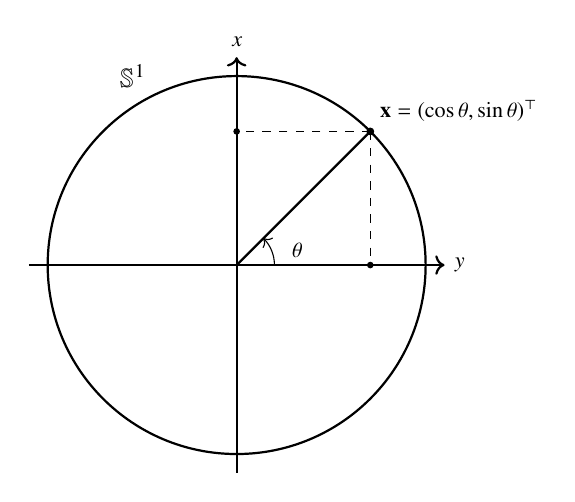
\begin{tikzpicture}[scale=2.4]
  \def\th{35}

     % -------------------------
     % LEFT: circle (\mathbb{S}^{1})
     % -------------------------
      \draw[thick] (0,0) circle(1);
    
      % Radius line
      \draw[thick] (0,0) -- ({cos(45)}, {sin(45)});
    
      % Axes
      \draw[->, thick] (-1.1,0) -- (1.1,0) node[right] {\footnotesize $y$};
      \draw[->, thick] (0,-1.1) -- (0,1.1) node[above] {\footnotesize $x$};
    
      % Coordinates
      \coordinate (P) at ({cos(45)}, {sin(45)});
      \coordinate (Px) at ({cos(45)}, 0);
      \coordinate (Py) at (0, {sin(45)});
    
      % Dashed projections
      \draw[dashed] (P) -- (Px);
      \draw[dashed] (P) -- (Py);
    
      % Labels near projection points (smaller text)
      \node[left] at ($(Py) + (-0.05, 0)$) {\footnotesize};
      \node[below] at ($(Px) + (0, -0.05)$) {\footnotesize};
    
      % Black dots at projection points
      \fill[black] (Px) circle(0.5pt);
      \fill[black] (Py) circle(0.5pt);
    
      % Point and radius
      \filldraw[black] (P) circle(0.5pt);
      \node[above right] at (P) {\footnotesize $\bx = (\cos\theta, \sin\theta)^\top$};
      \node[right] at ($(P)!0.5!(0,0)$) {\footnotesize};
    
      % Angle theta
      \draw[->] (0.2,0) arc[start angle=0,end angle=45,radius=0.2];
      \node at (0.32,0.08) {\footnotesize $\theta$};
      % Space label
      \node at (-0.55,1) {$\mathbb{S}^{1}$};
\end{tikzpicture}
\end{minipage}\hfill
\begin{minipage}{0.50\textwidth}
\centering
\tdplotsetmaincoords{70}{110}
\begin{tikzpicture}[scale=3,tdplot_main_coords]
  % -------------------------
  % RIGHT: sphere (\mathbb{S}^{2}) -- shifted
  % -------------------------
  
  \def\th{40} %azimuth
  \def\ph{50} %polar angle (from +x3)

   % Spherical wedge (first octant) + outline
  \path[fill=gray!20,opacity=0.5]
    plot[variable=\t,domain=0:90,samples=30] ({cos(\t)},{sin(\t)},0) --
    plot[variable=\t,domain=0:90,samples=30] (0,{cos(\t)},{sin(\t)}) --
    plot[variable=\t,domain=90:0,samples=30] ({cos(\t)},0,{sin(\t)}) -- cycle;

  \draw[thick] plot[variable=\t,domain=0:90,samples=30] ({cos(\t)},{sin(\t)},0);
  \draw[thick] plot[variable=\t,domain=0:90,samples=30] (0,{cos(\t)},{sin(\t)});
  \draw[thick] plot[variable=\t,domain=0:90,samples=30] ({cos(\t)},0,{sin(\t)});

  \node at (0.55,-0.15,1) {$\mathbb{S}^{2}$};

  % Axes
  \draw[->, thick] (0,0,0) -- (1.25,0,0) node[anchor=north east] {$x$};
  \draw[->, thick] (0,0,0) -- (0,1.25,0) node[anchor=north west] {$y$};
  \draw[->, thick] (0,0,0) -- (0,0,1.25) node[anchor=south] {$z$};
   
  % Point on sphere (uses x = (cosθ sinφ, sinθ sinφ, cosφ))
  \tdplotsetcoord{P}{1}{\ph}{\th}
  \draw[thick] (0,0,0) -- (P);
  \fill (P) circle(0.6pt);
  
  % Dashed guides
  \draw[dashed] (P) -- (Pxy);
  \draw[dashed] (Pxy) -- (0,0,0);
  
  % Theta in xy-plane
  \tdplotdrawarc[->]{(0,0,0)}{0.35}{0}{\th}{}{}
  \node at (0.5,0.15,0) {$\theta$};
  
  % Phi in plane at fixed theta
  \tdplotsetthetaplanecoords{\th}
  \begin{scope}[tdplot_rotated_coords]
    \tdplotdrawarc[->]{(0,0,0)}{0.35}{0}{\ph}{}{}
    \node at (0.35,0.05,0.05) {$\varphi$};
  \end{scope}
  
  % Label formula near the point
  \node[anchor=west] at ($(P)+(0.05,0.05,0.05)$)
    {\footnotesize $\bx=(\cos\theta\sin\varphi,\ \sin\theta\sin\varphi,\ \cos\varphi)^\top$};
\end{tikzpicture}
\end{minipage}

\caption{\centering Polar coordinates on $\mathbb{S}^{1}$ (left) and spherical coordinates on $\mathbb{S}^{2}$ (right).}
\label{fig:circle-sphere}
\end{figure}

A key challenge in directional data analysis is that statistical methods must respect the geometry of $\mathbb{S}^d$. Since it is a compact manifold embedded in $\mathbb{R}^{d+1}$, classical Euclidean procedures cannot always be applied directly; basic summaries may yield outputs that do not lie on $\mathbb{S}^d$ and therefore lack a directional interpretation (see \citep{Mardia1999} for further details). A natural strategy for handling this constraint is to approximate the sphere locally by a linear space, as formalized by the tangent-normal decomposition.

\begin{comment}
\subsection*{Measures of location and dispersion}

A key challenge in directional data analysis is that statistical methods must respect the geometry of $\mathbb{S}^d$. Since it is a compact manifold embedded in $\mathbb{R}^{d+1}$, classical Euclidean procedures cannot always be applied directly: basic summaries may yield outputs that do not lie on $\mathbb{S}^d$ and therefore lack a directional interpretation. This difficulty arises even in the simplest case, $\mathbb{S}^1$, when defining an appropriate sample mean direction. Given $\bx_1, \dots, \bx_n\in\mathbb{S}^1$, with $\bx_i=(\cos\theta_i, \sin\theta_i)^\top$, a first attempt is to compute the Euclidean mean $\bar{\bx}=\frac{1}{n}\sum_{i=1}^n \bx_i$. However, $\mathbb{S}^1$ is not closed under addition or scalar multiplication, so $\bar{\bx}$ need not lie on the circle. For example, taking $\bx_1=(1,0)^\top$ and $\bx_2=(0,1)^\top$ gives $\bar{\bx}=\bigl(\tfrac{1}{2},\tfrac{1}{2}\bigr)^\top$, with $\|\bar{\bx}\|=\frac{1}{\sqrt{2}}<1$. An alternative is to work in polar coordinates by computing the arithmetic mean of the angles $\theta_1,\dots,\theta_n\in[0,2\pi)$ 
as $\bar{\theta}=\frac{1}{n} \sum_{i=1}^n \theta_i$, and set the directional mean as $(\cos\bar{\theta},\sin\bar{\theta})^\top\in
\mathbb{S}^1$. While this guarantees a point on $\mathbb{S}^1$, it ignores the periodicity of angles. For instance, $\theta_1=\frac{\pi}{3}$ and $\theta_2=\frac{5\pi}{3}$ give $\bar{\theta}=
\pi$, which points in the opposite direction of the true mean angle $0$.

These difficulties are addressed by computing the Euclidean mean in $\mathbb{R}^{d+1}$ and projecting the result onto $\mathbb{S}^d$ through normalization to unit length. The sample mean direction $\hat{\bmu}$ is thus defined as
\begin{equation}
    \label{eq:direct-mean}
    \hat{\bmu}=\frac{\bar{\bx}}{\|\bar{\bx}\|},
\end{equation}
provided $\bar{\bx}\neq \mathbf{0}$; if $\bar{\bx}=\mathbf{0}$, no unique direction is determined and the sample mean direction is 
undefined \citep[see Section~9.2 of][]{Mardia1999}. In addition, $\bar{R}=\|\bar{\bx}\|\in [0,1]$ is known as the mean resultant length, which measures the concentration of the observations around $\hat{\bmu}$, with values close to one indicating strong concentration (low dispersion) and values close to zero indicating high dispersion or no preferred direction. For further details, see \citep{Mardia1999}.

While the mean direction and mean resultant length offer a global summary of directional observations, many statistical procedures require a local description of the geometry of $\Sd$. A key tool for this purpose is the tangent-normal decomposition, which plays a central role in distribution theory and data analysis on  the hypersphere.


% \begin{figure}[!ht]
% \centering
% \begin{tikzpicture}[scale=1.3]
%   \def\r{1}
%   \def\angA{60}    % pi/3
%   \def\angB{300}   % 5pi/3

%   % Colors
%   \colorlet{obsBlue}{cyan!60!blue!70}
%   \colorlet{meanBlue}{blue!40}     % naive mean at pi
%   \colorlet{trueGreen}{green!45}   % true mean at 0

%   % Circle
%   \draw[thick] (0,0) circle(\r);

%   % Reference points and labels
%   \fill (0,\r) circle(1.1pt);
%   \fill (0,-\r) circle(1.1pt);
%   \node[above=2pt] at (0,\r) {\large $\frac{\pi}{2}$};
%   \node[below=2pt] at (0,-\r) {\large $\frac{3\pi}{2}$};

%   % True mean direction at 0 (green)
%   \fill[trueGreen] (\r,0) circle(1.6pt);
%   \draw[->,trueGreen,very thick] (0,0) -- (\r,0);
%   \node[right=3pt,trueGreen] at (\r,0) {\large $0$};

%   % Naive mean direction at pi (blue)
%   \fill[meanBlue] (-\r,0) circle(1.6pt);
%   \draw[->,meanBlue,very thick] (0,0) -- (-\r,0);
%   \node[left=3pt,meanBlue] at (-\r,0) {\large $\pi$};

%   % Observations (pink)
%   \coordinate (P1) at ({\r*cos(\angA)},{\r*sin(\angA)});
%   \coordinate (P2) at ({\r*cos(\angB)},{\r*sin(\angB)});

%   \draw[->,obsBlue,very thick] (0,0) -- (P1);
%   \draw[->,obsBlue,very thick] (0,0) -- (P2);

%   \fill[obsBlue] (P1) circle(1.6pt);
%   \fill[obsBlue] (P2) circle(1.6pt);

%   \node[above right=2pt,obsBlue] at (P1) {\large $\frac{\pi}{3}$};
%   \node[below right=2pt,obsBlue] at (P2) {\large $\frac{5\pi}{3}$};
% \end{tikzpicture}
% \caption{Failure of the arithmetic mean for circular data: the two observations at $\pi/3$ and $5\pi/3$ (blue) have arithmetic mean $\pi$ (blue), even though the natural mean direction is $0$ (green).}
% \label{fig:mean-error}
% \end{figure}
\end{comment}

%-----------------------------------------------------------------------------
\begin{comment}
An appropriate measure of location for independent directional observations $\bx_1,\dots,\bx_n \in \mathbb{S}^d$ is obtained by first averaging the observations in the Euclidean space $\mathbb{R}^{d+1}$, obtaining Euclidean sample mean vector, $\bar{\bx}$, and then projecting this vector onto $\Sd$ in the Euclidean sense, that is, normalizing it to unit length. That is, the sample mean direction, $\hat{\bmu}$, is defined as: 
\begin{equation}
    \label{eq:direct-mean}
    \hat{\bmu}=\frac{\bar{\bx}}{\|\bar{\bx}\|}.
\end{equation}
for $\bar{\bx}\neq \mathbf{0}$. Formally, define the resultant vector 
\begin{equation*}
    \mathbf{R} = \sum_{i = 0}^{n} \bx_i
\end{equation*}
which represents the vector sum of all observations in $\mathbb{R}^{d+1}$. Its direction indicates the overall orientation of the sample, while its length measures how strongly the observations are concentrated around that orientation. The associated Euclidean sample mean vector is then defined as
\begin{equation}
    \label{eq:mean-vec}
    \bar{\bx}=\frac{1}{n}\sum_{i=1}^{n}\bx_i= \frac{1}{n} \mathbf{R}.
\end{equation}

Thus, $\bar{\bx}$ is the rescaled version of the resultant vector. Since scaling does not affect direction, $\mathbf{R}$ and $\bar{\bx}$ have the same orientation.


To obtain a valid direction on $\Sd$, it is necessary to preserve the orientation of $\bar{\bx}$ while enforcing the unit norm constraint. In Euclidean geometry, the projection of a point onto a set is defined as the point in that set that minimizes Euclidean distance. Accordingly, the projection of $\bar{\bx}$ onto $\Sd$ is defined as the unit vector $\bmu\in\mathbb{S}^d$ that minimizes the distance to $\bar{\bx}$ that is, 
\begin{equation*}
\hat{\bmu} =
\arg\min_{\bmu\in\mathbb{S}^d} \|\bmu-\bar{\bx}\|^2.
\end{equation*}
When $\bar{\bx}\neq \mathbf{0}$, this minimizer is unique, because among all unit vectors, only the one pointing in the same direction as $\bar{\bx}$ achieves the smallest Euclidean distance.

Indeed, expanding the squared norm yields $\|\bmu-\bar{\bx}\|^2 = \|\bmu\|^2+\|\bar{\bx}\|^2-2\bmu^\top\bar{\bx}$. Since $\bmu\in\mathbb{S}^d$, it follows that $\|\bmu\|=1$, and thus $\|\bmu-\bar{\bx}\|^2= 1+\|\bar{\bx}\|^2-2\bmu^\top\bar{\bx}$. The first two terms are constant with respect to $\bmu$, so minimizing $\|\bmu-\bar{\bx}\|^2$ over $\Sd$ is equivalent to maximizing $\bmu^\top\bar{\bx}$ over $\Sd$. By the Cauchy--Schwarz inequality,
\begin{equation*}
\bmu^\top \bar{\bx} \le
\|\bmu\|\,\|\bar{\bx}\| = \|\bar{\bx}\|,  
\end{equation*}
with the equality holding if and only if $\bmu$ and $\bar{\bx}$ are linearly dependent, that is, when $\bmu$ is proportional to $\bar{\bx}$. Hence, provided that $\bar{\bx}\neq\mathbf{0}$, the maximum of $\bmu^\top\bar{\bx}$ over $\Sd$ is attained when $\bmu$ has the same direction as $\bar{\bx}$. Since $\bmu$ must have unit norm, the unique minimizer is given by \eqref{eq:direct-mean} \citep[see][]{Mardia1999}. If instead $\bar{\bx}=\mathbf{0}$ (equivalently, $\mathbf{R}=\mathbf{0}$), then every point on $\Sd$ is at the same distance from $\bar{\bx}$, so the projection is not unique, and the sample mean direction is undefined.  

Notice that $\bar{\bx}$ can be expressed in terms of its length and its direction as $\bar{\bx} = \bar{R} \hat{\bmu}$ where $\bar{R} =\|\bar{\bx}\| $ is called the mean resultant length. Since $\bar{\bx} = \frac{\mathbf{R}}{n}$ (see \eqref{eq:mean-vec}), it follows that 
\begin{equation*}
    \bar{R} = \frac{\|\mathbf{R}\|}{n}
\end{equation*}

Because each observation $\bx_i$ has unit length by the triangle inequality 
\begin{equation*}
    \| \mathbf{R}\| = \| \sum_{i = 1}^{n} \bx_i\| \leq \sum_{i = 1}^{n} \|\bx_i\| = n
\end{equation*}
which implies that $0\leq\bar{R}\leq1$. 
\end{comment}
%-----------------------------------------------------------------------------

\subsection*{Tangent--normal decomposition}

Since $\Sd$ is not a linear space, the sum of two points on $\Sd$ does not remain on the hypersphere, nor does scalar multiplication preserve the unit-norm constraint. However, in a neighborhood of a fixed reference direction $\bmu\in\Sd$, the sphere can be approximated by its tangent space at $\bmu$,  providing a natural way to recover a local linear structure. 

Let $\mathcal{T}_{\bmu} := \{\mathbf{u} \in \mathbb{R}^{d+1} : \norm{\bu} =1, \bmu^\top \mathbf{u} = 0\}$ denote the tangent space to $\Sd$ at $\bmu$, and let $\operatorname{span}(\bmu) := \{\lambda\bmu : \lambda \in \mathbb{R}\}$ denote the subspace generated by $\bmu$. Since $\mathcal{T}_{\bmu}$ is precisely the orthogonal complement of $\operatorname{span}(\bmu)$ in $\mathbb{R}^{d+1}$, every vector in $\mathbb{R}^{d+1}$ decomposes uniquely into a component parallel to $\bmu$ and a component lying in $\mathcal{T}_{\bmu}$. In particular applying this decomposition to $\bx\in\mathbb{S}^d \subset \mathbb{R}^{d+1}$ yields the tangent--normal decomposition 
\begin{equation}
\label{eq:tangent-normal}
\bx=t\bmu+\sqrt{1-t^2}\,\bzeta,
\end{equation}
where
\begin{equation*}
    t=\bmu^\top\bx\in(-1,1)
    \qquad\text{and}\qquad
    \bzeta=\frac{\bx-t\bmu}{\sqrt{1-t^2}} \in \mathcal{T}_{\bmu}.
\end{equation*}
Here, the term $t\bmu$ is the component of $\bx$ along the normal direction $\bmu$, whereas $\bx-t\bmu$ is the component orthogonal in $\mathcal{T}_{\bmu}$.



To express the tangential component $\bzeta$ in a concrete coordinate system, note that $\mathcal{T}_{\bmu}$ is a $d$-dimensional linear subspace of $\mathbb{R}^{d+1}$ and therefore has an orthonormal basis $\{\mathbf{b}_1,\dots,\mathbf{b}_d\}$. Let $\bB_{\bmu}:=(\mathbf{b}_1, \dots, \mathbf{b}_d) \in\mathbb{R}^{(d+1)\times d}$ be the matrix whose columns are these basis vectors, so that $\bB_{\bmu}^\top\bB_{\bmu}=I_d$. Furthermore, since $\mathbb{R}^{d+1}=\operatorname{span}(\bmu)\oplus\mathcal{T}_{\bmu}$, where $\oplus$ denotes the orthogonal direct sum, the orthogonal projector onto $\mathcal{T}_{\bmu}$ can be expressed as $\bB_{\bmu}\bB_{\bmu}^\top=I_{d+1}-\bmu\bmu^\top$. Thus, every vector $\mathbf u\in\mathcal{T}_{\bmu}$ can be written uniquely as $\mathbf u=\bB_{\bmu}\mathbf a$ for some $\mathbf a\in\mathbb{R}^d$. In particular, every unit tangent vector $\bzeta$ can be written as
\begin{equation}
    \label{eq:zeta_def}
    \bzeta=\bB_{\bmu}\bxi, \qquad \bxi\in\Sdm.
\end{equation}
Then, $\bxi$ may be interpreted as the coordinate vector of the tangent direction $\bzeta$ with respect to the chosen orthonormal basis of $\mathcal{T}_{\bmu}$. Substituting \eqref{eq:zeta_def} into \eqref{eq:tangent-normal}, the tangent--normal decomposition can equivalently be written as: 
\begin{equation}
\label{eq:tangent-normal-basis}
\bx=t\bmu+\sqrt{1-t^2}\,\bB_{\bmu}\bxi,
\qquad t\in(-1,1),\quad \bxi\in\Sdm.
\end{equation}

Therefore, \eqref{eq:tangent-normal-basis} represents each observation $\bx\in\mathbb{S}^d$ by a normal coordinate $t$ and a tangential coordinate $\bxi\in\Sdm$ relative to the basis determined by $\bB_{\bmu}$. Geometrically, $t=\bmu^\top\bx$ is the signed length of the orthogonal projection of $\bx$ onto the direction $\bmu$, so that $t\bmu$ is the normal component of $\bx$. The remaining term, $\sqrt{1-t^2}\,\bB_{\bmu}\bxi=\bx-t\bmu$, is orthogonal to $\bmu$ and therefore lies in the tangent space $\mathcal{T}_{\bmu}$. Figure~\ref{fig:tangent-normal} illustrates this decomposition in $\mathbb{S}^2$.

\begin{figure}[!ht]
\centering
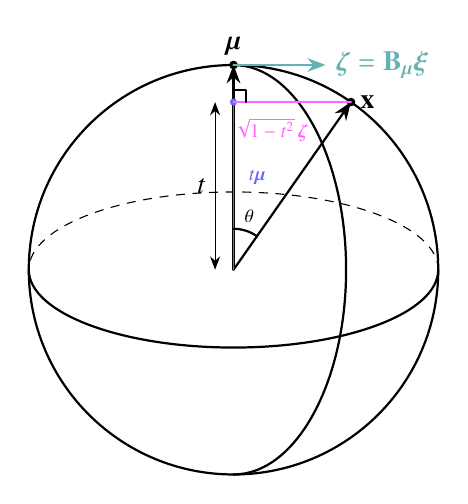
\begin{tikzpicture}[scale=1.3, line cap=round, line join=round, >=Stealth]

  \def\R{2.0}          % sphere radius (drawing)
  \def\eq{0.38}        % equator flattening (visual only)
  \def\alpha{35}       % polar angle from +z (in degrees)

  % Key points
  \coordinate (O)   at (0,0);
  \coordinate (mu)  at (0,\R);
  \coordinate (x)   at ({\R*sin(\alpha)},{\R*cos(\alpha)});
  \coordinate (tmu) at (0,{\R*cos(\alpha)});

  % Colors (optional; keep subtle)
  \colorlet{obsBlue}{magenta!55}
  \colorlet{meanBlue}{blue!45}
  \colorlet{trueGreen}{green!45}

  % Sphere outline
  \draw[thick] (O) circle(\R);

  % Equator (back dashed, front solid)
  \draw[dashed]  (\R,0) arc[start angle=0,   end angle=180, x radius=\R, y radius={\eq*\R}];
  \draw[thick] (-\R,0) arc[start angle=180, end angle=360, x radius=\R, y radius={\eq*\R}];

  % A meridian for 3D feel (back dashed, front solid)
  \draw[dashed] (0,-\R) arc[start angle=-90, end angle=90,  x radius={0.55*\R}, y radius=\R];
  \draw[thick]  (0,\R)  arc[start angle=90,  end angle=-90, x radius={0.55*\R}, y radius=\R];

  % mu (normal direction)
  \draw[->,thick] (O) -- (mu);
  \fill (mu) circle(1.2pt);
  \node[above] at (mu) {$\bmu$};

  % x (unit vector on the sphere)
  \draw[->, thick] (O) -- (x);
  \fill (x) circle(1.2pt);
  \node[right] at (x) {$\bx$};

  % % Normal component: t mu
  % \draw[very thick] (O) -- (tmu);
  % \fill (tmu) circle(1.0pt);
  % \node[right=2pt] at ($(O)!0.55!(tmu)$) {$t\bmu$};

  % Normal component: t mu (thinner, colored)
  \colorlet{normalCol}{blue!60}

  \draw[semithick, normalCol] (O) -- (tmu);
  \fill[normalCol] (tmu) circle(1.0pt);
  \node[right=2pt, text=normalCol, font=\scriptsize] at ($(O)!0.55!(tmu)$) {$t\bmu$};


  % Show t as a length (offset a bit to the left)
  \draw[<->] (-0.18,0) -- (-0.18,{\R*cos(\alpha)}) node[midway,left] {$t$};

  % Tangent component: sqrt(1-t^2) xi (no arrow, thinner, colored)
  \colorlet{tangentCol}{magenta!60}

  \draw[thick, tangentCol] (tmu) -- (x)
    node[pos=0.55, below, xshift=-10pt, yshift=-2pt, font=\scriptsize, text=tangentCol]
    {$\sqrt{1-t^2}\,\bzeta$};
    
  % Right angle marker at the decomposition corner
  \draw[thick] ($(tmu)+(0.12,0)$) -- ++(0,0.12) -- ++(-0.12,0);

  \colorlet{xiCol}{teal!60}
  % Unit tangent direction at mu
  \draw[->,thick, xiCol] (mu) -- ++(0.9,0) node[right] {$\bzeta = \bB_{\bmu}\bxi$};
  
  % Angle between \bmu and \bx: theta
 \draw[thick] (0,0.4) arc[start angle=90, end angle={90-\alpha}, radius=0.4];
 \node at ({0.5*cos(90-\alpha/2)},{0.55*sin(90-\alpha/2)}) {\scriptsize $\theta$};

\end{tikzpicture}
\caption{Tangent--normal decomposition on the sphere: $\bx=t\bmu+\sqrt{1-t^2}\,\bzeta$, where $t=\bmu^\top\bx$ and $\bzeta$ is a unit tangent vector at $\bmu$ with $\bmu^\top\bzeta=0$.}
\label{fig:tangent-normal}
\end{figure}


In addition, let $\sigmad$ denote the surface measure on $\Sd$, and let
\begin{equation}
\label{eq:omega-d}
\omega_d := \sigmad(\mathbb{S}^d)
= \frac{2\pi^{d+1/2}}{\Gamma\!\left({d+1}/{2}\right)}
\end{equation}
be the total surface area of $\Sd$ where $\Gamma$ denotes the gamma function given by $\Gamma(z) = \int_{0}^{\infty} t^{z-1}e^{-t} \,dt$ for $z\in \mathbb{C}$ such that $\operatorname{Re}(z) > 0$. Throughout this work, all integrals over $\Sd$ are taken with respect to $\sigmad$. The parametrization induced by the tangent--normal decomposition in \eqref{eq:tangent-normal-basis} yields a convenient change of variables for integration on the sphere given by \citet[Lemma~B.4]{Garcia-Portugues2014}. More precisely, for any function $f$ defined in $\Sd$, and any fixed reference direction $\bmu\in\mathbb{S}^d$,
\begin{equation*}
\label{eq:change-variable-sphere}
\int_{\mathbb{S}^d} f(\bx)\,\rd\sigmad(\bx)
=
\int_{-1}^{1}\int_{\Sdm}
f\!\left(t\bmu+\sqrt{1-t^2}\,\bB_{\bmu}\bxi\right)
(1-t^2)^{d/2-1}\,
d\sigmadm(\bxi)\,dt.
\end{equation*}

%This change of variables is a fundamental tool in directional statistics, as it directly enables the calculation of the normalizing constants and expectations required to define probability distributions on $\Sd$. 

\begin{comment}
For many procedures in directional data analysis, it is useful to work with a local linear approximation of the sphere. Although $\Sd$ is embedded in $\mathbb{R}^{d+1}$, it is not itself a linear space: in general, the sum of two points on $\Sd$ does not remain on the sphere, nor does scalar multiplication preserve the unit-norm constraint. However, in a neighborhood of a fixed reference direction $\bmu\in\Sd$, the sphere can be approximated by its tangent space at $\bmu$. 

%Let $\mathcal{T}_{\bmu} := \{\mathbf{u} \in \mathbb{R}^{d+1}:\bmu^\top \mathbf{u} = 0\}$ denote the tangent space to $\mathbb{S}^d$ at $\bmu$, and let $\operatorname{span}(\bmu) := \{\lambda\bmu : \lambda \in \mathbb{R}\}$ denote the one-dimensional subspace of $\mathbb{R}^{d+1}$ generated by $\bmu$. Since it is defined by a single independent linear constraint, $\mathcal{T}_{\bmu}$ is a $d$-dimensional linear subspace of $\mathbb{R}^{d+1}$. Moreover, because $\mathcal{T}_{\bmu}$ consists of all vectors in $\mathbb{R}^{d+1}$ orthogonal to $\bmu$, it is precisely the orthogonal complement of the one-dimensional subspace $\operatorname{span}(\bmu)$. Consequently, every vector in $\mathbb{R}^{d+1}$ can be written uniquely as the sum of a component parallel to $\bmu$ and a component lying in $\mathcal{T}_{\bmu}$. 


Let $\mathcal{T}_{\bmu} := \{\mathbf{u} \in \mathbb{R}^{d+1} : \bmu^\top \mathbf{u} = 0\}$ denote the tangent space to $\mathbb{S}^d$ at $\bmu$, and let $\operatorname{span}(\bmu) := 
\{\lambda\bmu : \lambda \in \mathbb{R}\}$ denote the subspace of $\mathbb{R}^{d+1}$ generated by $\bmu$. Since $\mathcal{T}_{\bmu}$ is defined by a single linear constraint, it is a $d$-dimensional subspace of $\mathbb{R}^{d+1}$, and precisely the orthogonal complement of $\operatorname{span}(\bmu)$. Consequently, every 
vector in $\mathbb{R}^{d+1}$ decomposes uniquely into a component parallel to $\bmu$ and a component lying in $\mathcal{T}_{\bmu}$.

More precisely, applying this orthogonal decomposition to an observation $\bx\in\mathbb{S}^d$ yields the tangent--normal decomposition n
\begin{equation}
\label{eq:tangent-normal}
\bx=t\bmu+\sqrt{1-t^2}\,\bzeta,
\end{equation}
where
\begin{equation*}
    t=\bmu^\top\bx\in(-1,1)
    \qquad\text{and}\qquad
    \bzeta=\frac{\bx-t\bmu}{\sqrt{1-t^2}}.
\end{equation*}
Here, the term $t\bmu$ is the component of $\bx$ along the normal direction $\bmu$, whereas $\bx-t\bmu$ is the component orthogonal to $\bmu$. Indeed, $\bmu^\top(\bx-t\bmu) = \bmu^\top\bx-t\,\bmu^\top\bmu = 0$, so $\bx-t\bmu\in\mathcal{T}_{\bmu}$. Moreover, since $\|\bx\|=\|\bmu\|=1$, it follows that
\begin{equation*}
    \|\bx-t\bmu\|^2 = (\bx-t\bmu)^\top(\bx-t\bmu) = \|\bx\|^2-2t\,\bmu^\top\bx+t^2\|\bmu\|^2 = 1-2t^2+t^2 = 1-t^2.
\end{equation*}
Therefore, 
\begin{equation*}
    \|\bzeta\| = \frac{\|\bx-t\bmu\|}{\sqrt{1-t^2}} = 1,
\end{equation*}
and hence $\bzeta\in\mathcal{T}_{\bmu}$ is a unit tangent vector.

As a $d$-dimensional linear subspace of $\mathbb{R}^{d+1}$, $\mathcal{T}_{\bmu}$ has an orthonormal basis, say $\{\mathbf b_1,\dots,\mathbf b_d\}$. Let $\bB_{\bmu}:=(\mathbf b_1,\dots,\mathbf b_d)\in\mathbb{R}^{(d+1)\times d}$ be the matrix whose columns are these basis vectors. Since the columns of $\bB_{\bmu}$ are orthonormal, it follows that $\bB_{\bmu}^\top \bB_{\bmu}=I_d$. Furthermore, because the column space of $\bB_{\bmu}$ is precisely $\mathcal{T}_{\bmu}$, the matrix $\bB_{\bmu}\bB_{\bmu}^\top$ is the orthogonal projector onto $\mathcal{T}_{\bmu}$. Using the identity $\mathcal{T}_{\bmu} =\operatorname{span}(\bmu)^\perp$, where $^\perp$ denotes the orthogonal complement in $\mathbb{R}^{d+1}$, this projector can be written as $\bB_{\bmu}\bB_{\bmu}^\top=I_{d+1}-\bmu\bmu^\top$.

Thus, $\bB_{\bmu}$ provides a coordinate representation of tangent vectors: every vector $\mathbf u\in\mathcal{T}_{\bmu}$ can be written uniquely as $\mathbf u=\bB_{\bmu}\mathbf a$ for some $\mathbf a\in\mathbb{R}^d$. In particular, since $\bB_{\bmu}^\top \bB_{\bmu}=I_d$, such a vector has unit norm if and only if $\|\mathbf a\|=1$. Hence, every unit tangent vector $\bzeta\in\mathcal{T}_{\bmu}$ can be represented uniquely as
\begin{equation}
    \label{eq:zeta_def}
    \bzeta=\bB_{\bmu}\bxi,
\qquad \bxi\in\Sdm.
\end{equation}

Then, $\bxi$ may be interpreted as the coordinate vector of the tangent direction $\bzeta$ with respect to the chosen orthonormal basis of $\mathcal{T}_{\bmu}$.Substituting \eqref{eq:zeta_def} into \eqref{eq:tangent-normal}, the tangent--normal decomposition can equivalently be written as: 
\begin{equation}
\label{eq:tangent-normal-basis}
\bx=t\bmu+\sqrt{1-t^2}\,\bB_{\bmu}\bxi,
\qquad t\in(-1,1),\quad \bxi\in\Sdm.
\end{equation}

Therefore, \eqref{eq:tangent-normal-basis} represents each observation $\bx\in\mathbb{S}^d$ by a normal coordinate $t$ and a tangential coordinate $\bxi\in\Sdm$ relative to the basis determined by $\bB_{\bmu}$. Geometrically, $t=\bmu^\top\bx$ is the signed length of the orthogonal projection of $\bx$ onto the direction $\bmu$, so that $t\bmu$ is the normal component of $\bx$. The remaining term, $\sqrt{1-t^2}\,\bB_{\bmu}\bxi=\bx-t\bmu$, is orthogonal to $\bmu$ and therefore lies in the tangent space $\mathcal{T}_{\bmu}$. Hence, this decomposition separates $\bx$ into a component along the reference direction $\bmu$ and a component describing its local departure from $\bmu$ within the tangent space. Figure~\ref{fig:tangent-normal} illustrates this decomposition in $\mathbb{S}^2$.

\begin{figure}[!ht]
\centering
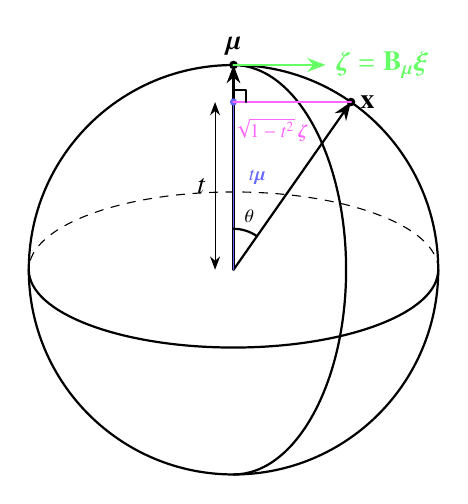
\begin{tikzpicture}[scale=1.3, line cap=round, line join=round, >=Stealth]

  \def\R{2.0}          % sphere radius (drawing)
  \def\eq{0.38}        % equator flattening (visual only)
  \def\alpha{35}       % polar angle from +z (in degrees)

  % Key points
  \coordinate (O)   at (0,0);
  \coordinate (mu)  at (0,\R);
  \coordinate (x)   at ({\R*sin(\alpha)},{\R*cos(\alpha)});
  \coordinate (tmu) at (0,{\R*cos(\alpha)});

  % Colors (optional; keep subtle)
  \colorlet{obsBlue}{magenta!55}
  \colorlet{meanBlue}{blue!45}
  \colorlet{trueGreen}{green!45}

  % Sphere outline
  \draw[thick] (O) circle(\R);

  % Equator (back dashed, front solid)
  \draw[dashed]  (\R,0) arc[start angle=0,   end angle=180, x radius=\R, y radius={\eq*\R}];
  \draw[thick] (-\R,0) arc[start angle=180, end angle=360, x radius=\R, y radius={\eq*\R}];

  % A meridian for 3D feel (back dashed, front solid)
  \draw[dashed] (0,-\R) arc[start angle=-90, end angle=90,  x radius={0.55*\R}, y radius=\R];
  \draw[thick]  (0,\R)  arc[start angle=90,  end angle=-90, x radius={0.55*\R}, y radius=\R];

  % mu (normal direction)
  \draw[->,thick] (O) -- (mu);
  \fill (mu) circle(1.2pt);
  \node[above] at (mu) {$\bmu$};

  % x (unit vector on the sphere)
  \draw[->, thick] (O) -- (x);
  \fill (x) circle(1.2pt);
  \node[right] at (x) {$\bx$};

  % % Normal component: t mu
  % \draw[very thick] (O) -- (tmu);
  % \fill (tmu) circle(1.0pt);
  % \node[right=2pt] at ($(O)!0.55!(tmu)$) {$t\bmu$};

  % Normal component: t mu (thinner, colored)
  \colorlet{normalCol}{blue!60}

  \draw[semithick, normalCol] (O) -- (tmu);
  \fill[normalCol] (tmu) circle(1.0pt);
  \node[right=2pt, text=normalCol, font=\scriptsize] at ($(O)!0.55!(tmu)$) {$t\bmu$};


  % Show t as a length (offset a bit to the left)
  \draw[<->] (-0.18,0) -- (-0.18,{\R*cos(\alpha)}) node[midway,left] {$t$};

  % Tangent component: sqrt(1-t^2) xi (no arrow, thinner, colored)
  \colorlet{tangentCol}{magenta!60}

  \draw[thick, tangentCol] (tmu) -- (x)
    node[pos=0.55, below, xshift=-10pt, yshift=-2pt, font=\scriptsize, text=tangentCol]
    {$\sqrt{1-t^2}\,\bzeta$};
    
  % Right angle marker at the decomposition corner
  \draw[thick] ($(tmu)+(0.12,0)$) -- ++(0,0.12) -- ++(-0.12,0);

  \colorlet{xiCol}{green!60}
  % Unit tangent direction at mu
  \draw[->,thick, xiCol] (mu) -- ++(0.9,0) node[right] {$\bzeta = \bB_{\bmu}\bxi$};
  
  % Angle between \bmu and \bx: theta
 \draw[thick] (0,0.4) arc[start angle=90, end angle={90-\alpha}, radius=0.4];
 \node at ({0.5*cos(90-\alpha/2)},{0.55*sin(90-\alpha/2)}) {\scriptsize $\theta$};

\end{tikzpicture}
\caption{Tangent--normal decomposition on the sphere: $\bx=t\bmu+\sqrt{1-t^2}\,\bzeta$, where $t=\bmu^\top\bx$ and $\bzeta$ is a unit tangent vector at $\bmu$ with $\bmu^\top\bzeta=0$.}
\label{fig:tangent-normal}
\end{figure}

An equivalent trigonometric form is obtained by letting $\theta\in[0,\pi]$ denote the angle between $\bmu$ and $\bx$. Since $\bmu,\bx\in\mathbb{S}^d$, the Euclidean angle formula gives $\cos\theta=\frac{\bmu^\top\bx}{\|\bmu\|\,\|\bx\|}=\bmu^\top\bx=t$. Therefore, $\sin\theta = \sqrt{1-t^2}$ and the tangent--normal decomposition in \eqref{eq:tangent-normal} can be written as
\begin{equation*}
    \bx = \bmu\cos\theta + \bxi\sin\theta.
\end{equation*}

In addition, let $\sigmad$ denote the surface measure on $\Sd$, and let
\begin{equation}
\label{eq:omega-d}
\omega_d := \sigmad(\mathbb{S}^d)
= \frac{2\pi^{\frac{d+1}{2}}}{\Gamma\!\left(\frac{d+1}{2}\right)}
\end{equation}
be the total surface area of $\Sd$ where $\Gamma$ denotes the gamma function given by $\Gamma(z) = \int_{0}^{\infty} t^{z-1}e^{-t} \,dt$ for $z\in \mathbb{C}$ such that $\operatorname{Re}(z) > 0$. The parametrization induced by the tangent--normal decomposition in \eqref{eq:tangent-normal-basis} yields a convenient change of variables for integration on the sphere given by \citet[Lemma~B.4]{Garcia-Portugues2014}. More precisely, for any function $f$ defined in $\Sd$, and any fixed reference direction $\bmu\in\mathbb{S}^d$,
\begin{equation*}
\label{eq:change-variable-sphere}
\int_{\mathbb{S}^d} f(\bx)\,\rd\sigmad(\bx)
=
\int_{-1}^{1}\int_{\Sdm}
f\!\left(t\bmu+\sqrt{1-t^2}\,\bB_{\bmu}\bxi\right)
(1-t^2)^{d/2-1}\,
d\sigmadm(\bxi)\,dt.
\end{equation*}

This change of variables is a fundamental tool in directional statistics, as it directly enables the calculation of the normalizing constants and expectations required to define probability distributions on $\Sd$.  
\end{comment}
\subsection*{Probability distributions on the sphere}

%A directional distribution is the distribution of a random variable $\bX$ taking values on $\mathbb{S}^d$. Because the unit sphere $\Sd$ is a non-linear manifold, standard Euclidean integration does not apply. To properly define a continuous probability distribution on the sphere, its density function $f$ must be specified with respect to an appropriate reference measure.  Consequently, $f$ is defined with respect to the $d$-dimensional Lebesgue surface measure, denoted by $\sigmad$. In addition, a valid spherical density $f$ must be non-negative, that is, $f(\bx) \geq 0$ for all $\bx \in \mathbb{S}^d$ and satisfy: 
A directional distribution is a probability distribution supported on $\mathbb{S}^d$, whose density $f$ with respect to $\sigmad$ satisfies $f(\bx)\geq 0$ for all $\bx\in\mathbb{S}^d$ and
\begin{equation*}
    \int_{\mathbb{S}^d} f(\bx)\,\rd\sigmad(\bx) = 1.
\end{equation*}

 


%A spherical distribution is the distribution of a random variable taking values on the unit sphere $\Sd$. Accordingly, probability is assigned to measurable subsets of $\Sd$, and any density must be defined with respect to a measure on the sphere itself. Since $\Sd$ is a non-linear manifold, the appropriate reference measure is the $d$-dimensional surface measure $\sigmad$. Throughout, all densities are taken with respect to $\sigmad$, normalized so that $\sigmad(\mathbb{S}^d)=\omega_d$, where $\omega_d$ is given in \eqref{eq:omega-d}. The following sections review the most commonly used probability distributions on the sphere.

The simplest distribution on $\Sd$ is the uniform distribution. A random vector $\mathbf X$ is uniformly distributed on $\Sd$ if it assigns equal probability to regions of equal surface area. Its density with respect to $\sigmad$ is therefore constant \citep{Ley2017a}: 
\begin{equation}
\label{eq:sph-uniform}
f(\bx)=\omega_d^{-1}, \qquad \bx\in\mathbb{S}^d,
\end{equation}
\begin{comment}
Therefore, the probability assigned to a measurable set $A\subseteq\mathbb{S}^d$ is proportional to its $d$-dimensional surface area, namely
\begin{equation*}
\mathbb{P}(X \in A) = \int_A f(\bx)\,\rd\sigmad(\bx) 
= \int_A \omega_d^{-1}\,\rd\sigmad(\bx) 
= \omega_d^{-1} \int_A 1\,\rd\sigmad(\bx) 
= \omega_d^{-1}\, \sigmad(A) 
= \frac{\sigmad(A)}{\omega_d}.
\end{equation*}
\end{comment}
For $d=1$, the normalizing constant $\omega_1 = 2\pi$ represents the total circumference of the unit circle $\mathbb{S}^1$. Consequently, the density of the uniform distribution on the circle simplifies to $f(\bx) = \frac{1}{2\pi}$, $\bx \in \mathbb{S}^1$. 

The most common directional distribution is the von Mises--Fisher or shortly von Mises distribution \citep[see][]{Watson1983, Mardia1999a}. For a random vector $\bx \in \Sd$, the density function of the von Mises--Fisher distribution, denoted by $\mathrm{vMF}(\bmu,\kappa)$, with respect to the surface measure $\sigmad$ is given by 
\begin{equation}
    \label{eq:vonMisesFisher}
    f(\bx; \bmu, \kappa) = C_{d}(\kappa)\exp\left\{ \kappa \bx^\top\bmu \right\}, \quad C_{d}(\kappa) = \frac{\kappa^{{d-1}/{2}}}{(2\pi)^{{d+1}/{2}} \mathcal{I}_{{d-1}{/2}}(\kappa)}
\end{equation}
where $\bmu \in \Sd$ is the mean direction and $\kappa \geq 0$ is the concentration parameter around the mean (where $\kappa = 0$ corresponds to the uniform distribution). $\mathcal{I}_{\nu}$ denotes the modified Bessel function of the first kind of order $\nu$ \citep[see][]{NIST:DLMF},
defined by 
\begin{equation*}
    I_{\nu}(\kappa) =
    \frac{(\kappa/2)^{\nu}}
    {\sqrt{\pi}\,\Gamma\!\left(\nu+1/2\right)}
    \int_{-1}^{1}
    e^{\kappa t}
    \left(1-t^{2}\right)^{\nu-\frac{1}{2}}
    \,\rd t.
\end{equation*}

The von Mises--Fisher density depends on $\bx$ only through the inner product $\bx^\top\bmu$, which means it is constant on all points at the same angular distance from $\bmu$, making the distribution rotationally symmetric around $\bmu$ and unimodal with a unique mode at $\bmu$. Moreover, $\kappa$ controls the concentration of the distribution around $\bmu$, being inversely related to the directional variance: large values of $\kappa$ tightly cluster the probability mass around $\bmu$, while a small $\kappa$ results in a high-variance distribution.

This distribution is the natural directional analogue of the Gaussian distribution, as its maximum likelihood estimator for the mean direction coincides with the directional sample mean \citep{Bingham1975}, and its density arises by projecting a normal vector $\mathbf{Z}\sim\mathcal{N}_{d+1}(\bmu_Z,\sigma^2\mathbf{I}_{d+1})$ onto $\Sd$, yielding $\mathbf{Y}=\mathbf{Z}/\|\mathbf{Z}\|\sim\mathrm{vMF}(\bmu_Z/\|\bmu_Z\|,\|\bmu_Z\|/\sigma^2)$, where $\kappa=\|\bmu_Z\|/\sigma^2$ plays the role of inverse variance \citep{Gatto2011}.

\begin{comment}

This distribution is usually regarded as the natural directional analogue of the Euclidean Gaussian distribution for two main reasons. First, it is the only directional distribution whose Maximum Likelihood Estimator (MLE) for the mean direction is the directional sample mean \citep{Bingham1975}, a property shared with the Gaussian distribution. Second, its density arises by conditioning a normal vector $\mathbf{Z} \sim \mathcal{N}_{d+1}
(\bmu_Z, \sigma^2\mathbf{I}_{d+1})$, with $\bmu_Z \in \mathbb{R}^{d+1} \setminus \{\mathbf{0}\}$ and $\sigma^2 > 0$, to have unit norm, yielding
\begin{equation*}
    \mathbf{Y} = \frac{\mathbf{Z}}{\norm{\mathbf{Z}}}\sim \mathrm{vMF}\!\left(\frac{\bmu_Z}{\|\bmu_Z\|}, 
    \frac{\|\bmu_Z\|}{\sigma^2}\right).
\end{equation*}

This shows that $\kappa$ plays the role of the inverse variance of the corresponding normal distribution: the more concentrated $\mathbf{Z}$ is around $\bmu_Z$ (smaller $\sigma^2$), the more concentrated $\mathbf{Y}$ is around $\bmu_Z/\|\bmu_Z\|$ (larger $\kappa = \|\bmu_Z\|/\sigma^2$) \citep[see][for a proof in the more general setting of the generalized von Mises--Fisher distribution on $\mathbb{S}^{d-1}$]{Gatto2011}
\end{comment}



%------------------------------------------------------------------------------
% 1) UNIFORM DISTRIBUTION
%------------------------------------------------------------------------------
\begin{comment}
The simplest distribution on $\Sd$ is the uniform distribution. A random vector $\mathbf X$ is uniformly distributed on $\Sd$ if it assigns equal probability to regions of equal surface area. Its density with respect to $\sigmad$ is therefore constant and given by \citet{Ley2017a}: 
\begin{equation}
\label{eq:sph-uniform}
f_{\mathbf X}(\bx)=\omega_d^{-1}, \qquad \bx\in\mathbb{S}^d,
\end{equation}
where $\omega_d=\sigmad(\mathbb{S}^d)$ denotes the total surface area of $\Sd$. Therefore, under this distribution, the probability assigned to a measurable set $A\subseteq\mathbb{S}^d$ is proportional to its $d$-dimensional surface area, namely
\begin{equation*}
\mathbb{P}(X \in A) = \int_A f_{\mathbf X}(\bx)\,\rd\sigmad(\bx) 
= \int_A \omega_d^{-1}\,\rd\sigmad(\bx) 
= \omega_d^{-1} \int_A 1\,\rd\sigmad(\bx) 
= \omega_d^{-1}\, \sigmad(A) 
= \frac{\sigmad(A)}{\omega_d}.
\end{equation*}

To illustrate this with a concrete example, consider the circular case, which corresponds to $d=1$. In this setting, the normalizing constant $\omega_1$ represents the total circumference of the unit circle $\mathbb{S}^1$ and is given by $
\omega_1 = \frac{2\pi^{\frac{1+1}{2}}}{\Gamma\left(\frac{1+1}{2}\right)} = \frac{2\pi}{\Gamma(1)} = 2\pi$. Consequently, the density of the uniform distribution on $\mathbb{S}^1$ simplifies to $f_{\mathbf X}(\bx) = \frac{1}{2\pi}$, $\bx \in \mathbb{S}^1$. 


As mentioned above, an important one-dimensional summary of a spherical random vector is its projection onto a fixed direction. Let $\bmu\in\mathbb{S}^d$ be fixed and define $T:=\bmu^\top\mathbf X \in (-1,1)$. This random variable is the scalar projection of $\mathbf X$ onto $\bmu$. By combining the tangent--normal parametrization in \eqref{eq:tangent-normal-basis} with the change-of-variables formula in \eqref{eq:change-variable-sphere}, the density of $T$ is obtained by integrating out the tangential coordinate $\bxi$:
\begin{equation*}
f_T(t)= \int_{\Sdm}
f_{\mathbf X}\!\left(t\bmu+\sqrt{1-t^2}\,\bB_{\bmu}\bxi\right)
(1-t^2)^{\frac d2-1}\,
d\sigmadm(\bxi),
\qquad -1\le t\le 1.
\end{equation*}

In the uniform case, $f_{\mathbf X}(\bx)=\omega_d^{-1}$ for all $\bx\in\mathbb{S}^d$, and therefore
\begin{align*}
f_T(t)
&=
\omega_d^{-1}(1-t^2)^{\frac d2-1}
\int_{\Sdm} d\sigmadm(\bxi) =\frac{\omega_{d-1}}{\omega_d}(1-t^2)^{\frac d2-1},
\qquad -1\le t\le 1.
\end{align*}
Hence, the projection of a uniformly distributed random vector on $\Sd$ onto any fixed direction $\bmu$ has density
\begin{equation*}
f_T(t)=\frac{\omega_{d-1}}{\omega_d}(1-t^2)^{\frac d2-1},
\qquad -1\le t\le 1.
\end{equation*}

This normalizing constant may be expressed in terms of the beta function, denoted as $B(x,y)$. Recall that, for $x,y>0$,
\begin{equation*}
B(x,y)=\int_0^1 u^{x-1}(1-u)^{y-1}\,du.
\end{equation*}

Since $f_T$ is a probability density, it must integrate to one over $[-1,1]$, so
\[
1=\frac{\omega_{d-1}}{\omega_d}\int_{-1}^1 (1-t^2)^{\frac d2-1}\,dt.
\]

Then, using the substitution $u=t^2$ (so $du=2t\,dt$) and symmetry about $0$, we obtain
\begin{align*}
\int_{-1}^{1} (1-t^2)^{\frac{d-2}{2}}\,dt
&=
2\int_{0}^{1} (1-t^2)^{\frac{d-2}{2}}\,dt
=
2\int_{0}^{1} (1-u)^{\frac{d-2}{2}}\frac{1}{2}u^{-1/2}\,du \\
&=
\int_{0}^{1} u^{-1/2}(1-u)^{\frac d2-1}\,du
=
B \left(\frac12,\frac d2\right).
\end{align*}

Therefore,
\[
\frac{\omega_{d-1}}{\omega_d}
=
B\!\left(\frac12,\frac d2\right)^{-1},
\]
and the density of $T$ can be written equivalently as
\begin{equation*}
f_T(t)
=
B\!\left(\frac12,\frac d2\right)^{-1}(1-t^2)^{\frac d2-1},
\qquad -1\le t\le 1.
\end{equation*}
\end{comment}

%------------------------------------------------------------------------------
% 2) VON MISES FISHER DISTRIBUTION
%------------------------------------------------------------------------------
\begin{comment}
    \subsubsection*{von Mises--Fisher distribution}
The most popular directional distribution is the von Mises--Fisher or shortly von Mises distribution \citep[see][]{Watson1983, Mardia1999a}. For a random vector $\bx \in \Sd$, the density function of the von Mises--Fisher distribution, denoted by $vM(\bmu,\kappa)$, with respect to the surface measure $\sigmad$ is given by 
\begin{equation}
    \label{eq:vonMisesFisher}
    f(\bx; \bmu, \kappa) = C_{d}(\kappa)\exp\left\{ \kappa \bx^\top\bmu \right\}, \quad C_{d}(\kappa) = \frac{\kappa^{\frac{d-1}{2}}}{(2\pi)^{\frac{d+1}{2}} \mathcal{I}_{\frac{d-1}{2}}(\kappa)}
\end{equation}
where $\bmu \in \Sd$ denotes the mean direction, $\kappa \geq 0$ the concentration parameter around the mean (where $\kappa = 0$ corresponds to the uniform distribution) and $\mathcal{I}_{\nu}$ denotes the modified Bessel function of the first kind of order $\nu$ \citep[see][]{NIST:DLMF},
defined by 
\begin{equation}
    I_{\nu}(\kappa) =
    \frac{\left(\frac{\kappa}{2}\right)^{\nu}}
    {\sqrt{\pi}\,\Gamma\!\left(\nu+\frac{1}{2}\right)}
    \int_{-1}^{1}
    e^{\kappa t}
    \left(1-t^{2}\right)^{\nu-\frac{1}{2}}
    \,\rd t.
\end{equation}

The von Mises--Fisher distribution is characterized by both the mean direction $\bmu \in \mathbb{S}^d$ and the concentration parameter $\kappa \ge 0$. On the one hand, a fundamental property of this distribution is that its density depends on the observation $\bx$ only through the inner product $\bx^\top\bmu$. Because both $\bx$ and $\bmu$ are unit vectors, this inner product is precisely the cosine of the angle $\theta$ between them. Hence, the density simplifies to $f(\bx; \bmu, \kappa) \propto \exp\{\kappa \cos\theta\}$. Consequently, the density is constant on sets of points with the same angular distance $\theta$ from $\bmu$. In other words, the distribution depends only on the distance to the mean direction, not on the specific direction of its deviation. This makes the distribution isotropic about $\bmu$ (rotationally symmetric): at a fixed $\theta$, all orientations around the axis defined by $\bmu$ are equally likely.


Moreover, for $\kappa\ge 0$ the exponential is strictly increasing, the density \eqref{eq:vonMisesFisher} is maximized when $\bx^\top\bmu=\cos\theta$ is maximized, which happens at $\theta=0$, that is, $\bx$ points exactly in the direction of $\bmu$ ($\bx=\bmu$). Because $\cos\theta$ decreases strictly for $\theta\in[0,\pi]$, the density $\exp{\kappa\cos\theta}$ decreases strictly as the angular distance from $\bmu$ increases. Hence, no other local maxima can occur, and the distribution is unimodal with a unique mode at $\bmu$.

Regarding its shape, the concentration parameter $\kappa \ge 0$ controls the dispersion of the data. It is inversely related to the directional variance: a large value of $\kappa$ tightly clusters the probability mass around the mean direction $\bmu$, while a small $\kappa$ results in a highly diffuse, high-variance distribution. Specifically, when $\kappa = 0$, the density becomes independent of the mean direction and is determined solely by the normalizing constant $C_d(0)$, perfectly recovering the uniform distribution on $\Sd$. Conversely, for any $\kappa > 0$, the distribution is unimodal and exhibits a clear preferred direction, concentrating increasingly heavily around $\bmu$ as $\kappa$ grows.

The von Mises--Fisher family is usually regarded as the natural directional analogue of the Euclidean Gaussian distribution \citep[see][]{Garcia-Portugues2014}. This equivalence is primarily supported by two fundamental mathematical properties. First, it shares the same Maximum Likelihood Estimator (MLE) characterization as the Gaussian distribution. Specifically, as shown by \citet{Bingham1975}, the von Mises--Fisher is the only directional distribution where the MLE for the mean direction $\bmu$ is the directional sample mean.

Second, the von Mises--Fisher density arises naturally by conditioning a multivariate Normal vector to lie on the unit hypersphere. Specifically, let $\mathbf{Z} \sim \mathcal{N}_{d+1}(\bmu_Z, \sigma^2 \mathbf{I}_{d+1})$ be an isotropic normal random vector in $\mathbb{R}^{d+1}$ with $\bmu_Z \in \mathbb{R}^{d+1} \setminus \{\mathbf{0}\}$ and $\sigma^2 > 0$. If we condition $\mathbf{Z}$ to have unit norm, the resulting random vector $\mathbf{Y} = (\mathbf{Z} : \|\mathbf{Z}\| = 1)$ follows a von Mises--Fisher distribution on $\Sd$, given by
\begin{equation*}
    \mathbf{Y} \sim vM\!\left(\frac{\bmu_Z}{\|\bmu_Z\|}, \frac{\|\bmu_Z\|}{\sigma^2}\right).
\end{equation*}

This result highlights that the inverse of the concentration parameter in a von Mises--Fisher distribution can be represented by the variance of a multivariate normal distribution with a spherical covariance matrix \citep[see][for a proof in a more generalized setting]{Gatto2011}.
\end{comment}

%------------------------------------------------------------------------------
% 3) FISHER--BINGHAM DISTRBUTION
%------------------------------------------------------------------------------
\begin{comment}
\subsubsection*{Fisher--Bingham distribution}
The Fisher--Bingham distribution generalizes the von Mises--Fisher model by augmenting the linear term $\kappa,\bx^\top\bmu$ with the quadratic form $\bx^\top\mathbf{A}\bx$, which allows for different dispersion along different directions rather than rotational symmetry about $\bmu$ \citep[see][]{Ley2018}. Its density on $\Sd$ with respect to surface area measure is
\begin{equation}
    \label{eq:fisherBingham}
    f(\bx;\bmu,\kappa,\mathbf{A})
    = \frac{1}{\alpha(\kappa,\mathbf{A})}
    \exp\!\left\{\kappa\,\bx^\top\bmu + \bx^\top\mathbf{A}\bx\right\},
    \qquad \bx\in\mathbb{S}^d,
\end{equation}
where $\bmu\in\mathbb{S}^d$ is the mean direction, $\kappa\ge 0$ is a concentration parameter, and $\mathbf{A}$ is a symmetric $(d+1)\times(d+1)$ matrix. The normalizing constant $\alpha(\kappa,\mathbf{A})$ ensures that the density integrates to one over $\Sd$, but approximating it is generally challenging; see, for example, \citet{Kume2005}. Because $\bx\in\mathbb{S}^d$ satisfies $\bx^\top\bx=1$, shifting $\mathbf{A}$ by a multiple of the identity does not change the shape of the density. Indeed, for any $c\in\mathbb{R}$,
\[
\bx^\top(\mathbf{A}+c\mathbf{I})\bx
= \bx^\top\mathbf{A}\bx + c\,\bx^\top\bx
= \bx^\top\mathbf{A}\bx + c,
\]
so
\[
\exp\{\kappa\,\bx^\top\bmu + \bx^\top(\mathbf{A}+c\mathbf{I})\bx\}
= e^{c}\exp\{\kappa\,\bx^\top\bmu + \bx^\top\mathbf{A}\bx\},
\]
and the constant factor $e^{c}$ can be absorbed into the normalizing constant $\alpha(\kappa,\mathbf{A})$. Hence $\mathbf{A}$ and $\mathbf{A}+c\mathbf{I}$ define the same distribution on $\Sd$. Notice that since $\mathbf{I}$ is $(d+1)\times(d+1)$, we have $\mathrm{tr}(\mathbf{I})=d+1$. Therefore, for any $c\in\mathbb{R}$, $\mathrm{tr}(\mathbf{A}+c\mathbf{I}) = \mathrm{tr}(\mathbf{A}) + c\,\mathrm{tr}(\mathbf{I}) = \mathrm{tr}(\mathbf{A}) + c(d+1)$. Therefore, without loss of generality, we can impose $\mathrm{tr}(\mathbf{A})=0$ by choosing $c=-\mathrm{tr}(\mathbf{A})/(d+1)$. 

Several standard directional models arise as special cases of the Fisher--Bingham distribution, under specific parameter choices. For instance, when $\mathbf{A}=\mathbf{0}$, the density in \eqref{eq:fisherBingham} reduces to the von Mises--Fisher density presented in \eqref{eq:vonMisesFisher}.  Alternatively, as noted by \citet{Jupp2009}, when the concentration parameter is $\kappa = 0$, the linear term vanishes, and the model becomes the Bingham distribution with density: 
\begin{equation*}
    f(\bx;\mathbf{A}) = {}_{1}F_{1}\left(\frac{1}{2}, \frac{d+1}{2}, \mathbf{A}\right)^{-1} \exp\{\bx^\top\mathbf{A}\bx\}, \qquad \bx\in\mathbb{S}^d,
\end{equation*}
where ${}_{1}F_{1}$ denotes the confluent hypergeometric function of a matrix argument. In this case, the hypergeometric function serves as the required normalizing constant to ensure the density integrates to unity over $\Sd$. A detailed discussion of this function is provided in Appendix 1 of \citet{Mardia1999}.
\end{comment}

%------------------------------------------------------------------------------
% 4) KENT DISTRIBUTION
%------------------------------------------------------------------------------
\begin{comment}
\subsubsection*{Kent distribution}

The Kent distribution is a special case of the Fisher--Bingham family, obtained by constraining the quadratic term to act only in directions orthogonal to the mean direction. Its density on $\Sd$ is
\begin{equation}
f(\bx;\bmu,\kappa,\mathbf A)
=
\frac{1}{a(\kappa,\mathbf A)}
\exp\!\left\{\kappa\,\bmu^\top\bx+\bx^\top \mathbf A \bx\right\},
\qquad \bx\in\mathbb{S}^d,
\end{equation}
where $\bmu\in\mathbb{S}^d$, $\kappa\ge 0$, and $\mathbf A$ is a symmetric $(d+1)\times(d+1)$ matrix satisfying
\[
\operatorname{tr}(\mathbf A)=0,
\qquad
\mathbf A\bmu=\mathbf 0.
\]
The condition $\mathbf A\bmu=\mathbf 0$ ensures that the quadratic term affects only directions tangent to the sphere at $\bmu$, while $\operatorname{tr}(\mathbf A)=0$ removes an irrelevant additive constant. Introduced by \citet{Kent1982}, this model extends the von Mises--Fisher distribution by allowing elliptical (or oval) contours around the modal direction $\bmu$, with $\mathbf A$ controlling the shape of the distribution.
\end{comment}

%------------------------------------------------------------------------------
% 5) MIXTURE MODELS
%------------------------------------------------------------------------------
\begin{comment}
\subsubsection*{Mixture distributions}

A mixture distribution provides a flexible framework for modeling complex data that cannot be adequately described by a single parametric family. Formally, a random vector $\bX$ follows an $r$-component mixture distribution if its density function $f$ can be expressed as a convex combination of $r$ component densities $\{f_1, \dots, f_r\}$, such that:
\begin{equation}
\label{eq:mixture-general}
f(\bx; \boldsymbol{\theta}) = \sum_{j=1}^{r} p_j f_j(\bx; \boldsymbol{\theta}_j),
\end{equation}
where $p_j > 0$ are the mixing weights satisfying $\sum_{j=1}^{r} p_j = 1$, and each $f_j$ is a valid probability density function with its own vector of parameters $\boldsymbol{\theta}_j$ \citep{McLachlan2000}.

In practice, directional observations are frequently multimodal and are thus often modeled using finite mixture distributions. Unlike their individual components, these mixtures generally do not belong to the exponential family, which complicates the use of standard inferential techniques \citep{Garcia-Portugues2021}.

For example, a common choice for modeling multimodal circular data is the mixture of von Mises (vM) distributions. An $r$-mixture of von Mises distributions on $\mathbb{S}^1$ has the density:
\begin{equation*}
f(\bx) = \sum_{j=1}^{r} p_j \text{vM}(\bx; \bmu_j, \kappa_j),
\end{equation*}
where each component is centered at a mean direction $\bmu_j$ with a concentration parameter $\kappa_j$. Such models are essential for analyzing phenomena like animal migration or wind patterns that exhibit multiple preferred orientations \citep{Mardia1999}.

In addition, when observations consist of both a directional component $\bx \in \mathbb{S}^d$ and a linear covariate $y \in \mathbb{R}$, mixtures of von Mises and Normal distributions are employed. In this scenario, the joint density is modeled as a mixture of product densities:
\begin{equation*}
f(\bx, y) = \sum_{j=1}^{r} p_j \text{vM}(\bx; \bmu_j, \kappa_j) \cdot \mathcal{N}(y; \beta_j, \sigma_j^2).
\end{equation*}
This approach allows the estimator to capture complex dependencies and distinct clusters within heterogeneous cylindrical data. 
\end{comment}

%So far, the focus has been on modeling directionaldata. However, in many practical applications, it is essential to understand how directional variables are related to other variables. This motivates the use of regression analysis, which aims to characterize the relationship between a response variable and one or more predictors. The following section provides an introduction to classical approaches for estimating regression functions in which a directional variable is involved. 



\section{Background on orthogonal polynomials} \label{sec:orthogonal}

%Puedes mirar DLMF-NIST o Szorgo (libro clásico de polinomios ortogonales).

Gegenbauer polynomials are a family of orthogonal polynomials on the space of square--integrable functions on $[-1,1]$ with respect to the weight function $w_d(x) = (1 - x^2)^{d/2 - 1}$, for $d \geq 2$ \citep[Section~4.7]{Szego1939}. This weighted space is usually denoted by $L_d^2([-1,1])$.  %\citep{Gar}. 

For $d \geq 2$, the Gegenbauer polynomials $\left\{C_k^{(d-1)/2}\right\}_{k=0}^{\infty}$, of index $\lambda = (d-1)/2$ \citep[Section~18.3]{NIST:DLMF}, form an orthogonal basis of $L_d^2([-1,1])$. This means that they are orthogonal with respect to the weighted inner product on $L_d^2([-1,1])$. More precisely, for any nonnegative integers $k$ and $\ell$,
\begin{equation*}
    \int_{-1}^{1} C_k^{(d-1)/2}(x) C_\ell^{(d-1)/2}(x)(1 - x^2)^{d/2 - 1}\,dx = \delta_{k,\ell}c_{k,d},\end{equation*}
where $\delta_{k,\ell}$ denotes the Kronecker delta and $c_{k,d}$ is the squared norm of the Gegenbauer polynomial $C_k^{(d-1)/2}$ in the weighted space $L_d^2([-1,1])$. More explicitly,
\begin{equation*}
\begin{aligned}
c_{k,d}
&:= \frac{2^{3-d}\pi \Gamma(d+k-1)}
{(d+2k-1)k!\Gamma((d-1)/2)^2} = \frac{\omega_d}{\omega_{d-1}}
\left(1+\frac{2k}{d-1}\right)^{-2} d_{k,d},
\end{aligned}
\end{equation*}
where
\begin{equation*}
\begin{aligned}
d_{k,d}
&:= \left(1+\frac{2k}{d-1}\right)
\frac{\Gamma(d-1+k)}{\Gamma(d-1)k!} = \left(1+\frac{2k}{d-1}\right) C_k^{(d-1)/2}(1).
\end{aligned}
\end{equation*}
Here, $C_k^{(d-1)/2}(1)$ denotes the value of the Gegenbauer polynomial $C_k^{(d-1)/2}(x)$ evaluated at $x=1$, $\omega_d$ denotes the surface area of the $d$-dimensional unit sphere given in \eqref{eq:omega-d}, and $d_{k,d}$ is the dimension of the vector space of spherical harmonics of degree $k$. 

The first Gegenbauer polynomials are $C_0^{(d-1)/2}(x) = 1$, $C_1^{(d-1)/2}(x) = (d - 1)x$, and $C_2^{(d-1)/2}(x) = \frac{d - 1}{2}\left((d + 1)x^2 - 1\right)$, while higher-degree polynomials can be generated recursively as \citep[Section~18.9]{NIST:DLMF}
\begin{equation*}
C_{k+1}^{(d-1) / 2}(x)=\frac{2 k+d-1}{k+1} 
\, x \, C_k^{(d-1) / 2}(x)-\frac{k+d-2}{k+1} \, C_{k-1}^{(d-1) / 2}(x), \quad k \geq 1 .
\end{equation*}
Since the Gegenbauer polynomials $\left\{C_k^{(d-1)/2}\right\}_{k=0}^{\infty}$ constitute an orthogonal basis for $L_d^2([-1,1])$, every $g \in L_d^2([-1,1])$ can be represented by its Gegenbauer series expansion
\begin{equation}
    \label{eq:Gegenbauer-series}
    g(x) = \sum_{k=0}^{\infty} b_{k,d}(g) \, C_k^{(d-1)/2}(x),
\end{equation}
where the Gegenbauer coefficients are given by
\begin{equation}
    \label{eq:gegenbauer_coeff}
    b_{k,d}(g)
    :=
    \frac{1}{c_{k,d}}
    \int_{-1}^{1}
    g(x) \, C_k^{(d-1)/2}(x)\,(1 - x^2)^{d/2 - 1}\,dx.
\end{equation}
The series  in \eqref{eq:Gegenbauer-series} converges in $L_d^2([-1,1])$.

This one-dimensional expansion has a direct interpretation for rotationally symmetric functions on the sphere \citep{Garcia-Portugues2026}. Suppose that $f \in L^2(\mathbb{S}^d)$ is rotationally symmetric about a fixed point $\bmu \in \mathbb{S}^d$. This means that applying any rotation that keeps $\bmu$ fixed does not change the value of the function. Equivalently, $f(\bx)$ depends only on the angle between $\bx$ and $\mu$, or, equivalently, on the scalar product $\bx^\top \bmu$. Therefore, there exists a function $g \in L_d^2([-1,1])$ such that
\begin{equation*}
    f(\bx) := g(\bx^\top \bmu),
    \qquad \bx \in \mathbb{S}^d.
\end{equation*}

Applying the Gegenbauer expansion of $g$ to the variable $\bx^\top \bmu \in [-1,1]$ in \eqref{eq:Gegenbauer-series}, the following expression is obtained
\begin{equation}
    \label{eq:spherical-harmonics}
    f(\bx) = \sum_{k=0}^{\infty}
    b_{k,d}(g) \, C_k^{(d-1)/2}(\bx^\top \bmu).
\end{equation}
which is the zonal spherical harmonics expansion of $f$ about $\mu$, which is convergent in $L^2(\mathbb{S}^d)$. 

Moreover, by \citet[Theorem 2]{Kalf1995}, this convergence can be assumed to be uniformly convergent whenever $f$ is sufficiently smooth. In particular, if $f \in C^\infty(\mathbb{S}^d)$, then the series in \eqref{eq:spherical-harmonics} is uniformly absolutely convergent.

% The term ``zonal'' reflects the fact that each function
% \[
%     x \mapsto C_k^{(d-1)/2}(x^\top \mu)
% \]
% is constant on the sets of points of $\Sd$ having the same inner product with $\mu$, or equivalently the same geodesic distance from $\mu$.


\section{Isotropic positive definite functions} \label{sec:isotropy}

This section reviews the basic theory of isotropic positive 
definite functions in Euclidean spaces and on spherical domains. 
Directional regression models with a spatial dependence structure 
arise naturally in many applied settings, including the study of 
extreme wind directions \citep{Coles1998} and the reconstruction 
of wave direction fields in oceanography \citep{Meilan-Vila2021a}, 
where in both cases observations at nearby locations tend to 
exhibit stronger dependence than those further apart. In such 
contexts, spatial dependence is described through a correlation 
function, which must be positive definite to guarantee a valid 
covariance structure for any finite collection of observation 
locations.

More precisely, function $h$ is said to be positive definite if, for every finite collection of distinct points $\bx_1,\ldots,\bx_k$ in the underlying domain, either a Euclidean space or a sphere, and for every set of constants $c_1,\ldots,c_k\in\mathbb{R}$, the following inequality holds
\citep{Gneiting2013}:
\begin{align}
    \label{eq:positive-definite}
    \sum_{i=1}^{k}\sum_{j=1}^{k} c_i c_j h(\bx_i,\bx_j)\geq 0.
\end{align}

%Concretely, $h$ is said to be strictly positive definite if the inequality in \eqref{eq:positive-definite} is strictly greater than zero for all nonzero coefficients $c_1,\ldots,c_k$.

Furthermore, according to \citet{Gneiting2013}, isotropy refers to the property that a function is invariant with respect to direction. In the present context, this means that the value of $h(\bx_i,\bx_j)$ depends only on the distance between two points, and not on the direction separating them. In spatial statistics, this property allows covariance and correlation functions to model dependence as a function of distance alone, reflecting the assumption that correlation decreases as the distance between locations increases.

%Such functions describe how the association between observations changes with distance, reflecting the assumption that correlation decreases as the distance between locations increases.

Positive definite functions are essential for constructing valid covariance structures \citep{Meilan-Vila2021a}. Combined with isotropy, they provide the mathematical foundation for modeling spatial dependence through distance alone, on both Euclidean and spherical domains.


%Positive definite functions are essential in the construction of covariance functions and in the study of relationships between values observed at different spatial locations \citet{Meilan-Vila2021a}. Combined with isotropy, positive definiteness ensures that spatial dependence can be modeled through distance-based covariance or correlation functions while still producing valid covariance matrices. Therefore, isotropic positive definite functions provide the mathematical foundation for describing spatial dependence. For this reason, the following discussion reviews basic results on isotropic positive definite functions in Euclidean spaces, before considering their restrictions to spherical domains.

A function $h:\mathbb{R}^d\times\mathbb{R}^d\to\mathbb{R}$ is called isotropic positive definite on $\mathbb{R}^d$ if it satisfies the positive definiteness condition in \eqref{eq:positive-definite} and, in addition, there exists a function $\varphi:[0,\infty)\to\mathbb{R}$ such that
\begin{equation}
    \label{eq:euclidean-iso}
     h(\bx,\by)=\varphi(\|\bx-\by\|),
    \qquad \bx,\by\in\mathbb{R}^d.
\end{equation}

Therefore, an isotropic positive definite function $h$ depends on two locations only through the Euclidean distance between them.

For $d \geq 1$, let $\Phi_d$ denote the class of continuous functions
$\varphi:[0,\infty)\to\mathbb{R}$ with $\varphi(0)=1$ such that the function $h$ defined in \eqref{eq:euclidean-iso} is positive definite on $\mathbb{R}^d$. Equivalently, $\Phi_d$ is the class of valid isotropic correlation functions on
$\mathbb{R}^d$ \citep{Gneiting2013}. Moreover, the classes $\Phi_d$ are nested and non-increasing with respect to the $d$:
\[
    \Phi_1 \supset \Phi_2 \supset \cdots \supset \Phi_\infty,
\]
where the inclusions are strict. Consequently, a function that is positive
definite in a higher-dimensional Euclidean space is also positive definite in
all lower-dimensional Euclidean spaces.

In addition, \citet{Schoenberg1938} showed that a function
$\varphi:[0,\infty)\to\mathbb{R}$ belongs to $\Phi_d$ if and only if it can be written as
\begin{equation*}
    %\label{eq:schoenberg-euclidean}
    \varphi(t) = \int_{[0,\infty)} \Omega_d(rt)\,dF(r), \qquad t\geq 0,
\end{equation*}
where $F$ is a uniquely determined probability measure (a probability distribution) on $[0,\infty)$ and
\begin{equation*}
    \Omega_d(t) = \Gamma\left(\frac{d}{2}\right)
    \left(\frac{2}{t}\right)^{(d-2)/2}
    J_{(d-2)/2}(t).
\end{equation*}
$J_{(d-2)/2}$ denotes the Bessel function of the first kind of order $(d-2)/2$, which can be defined, for a general order $\alpha$, by
\begin{equation*}
    J_{\alpha}(z) = \frac{1}{\pi} \int_{0}^{\pi} \cos\left(\alpha \tau - z\sin\tau\right)\,d\tau - \frac{\sin(\alpha\pi)}{\pi} \int_{0}^{\infty} e^{-z\sinh\tau-\alpha\tau}\,d\tau,
\end{equation*}
for $z\in\mathbb{C}$ such that $\operatorname{Re}(z)>0$.

%However, when spatial data are observed on curved surfaces, the Euclidean distance is often no longer the most appropriate way to measure the distance between two observations.  Consequently, the covariance structure should be defined in a way that reflects the geometry of the underlying space. 

However, when observations lie on a curved surface, Euclidean distance is no longer appropriate and the covariance structure must reflect the geometry of the underlying space. On the sphere $\Sd$, the  distance between two observations is
geodesic distance:
\begin{equation}
    \label{eq:spherical-distance}
    d_{G}(\bx,\by) = \arccos(\bx^\top\by), \qquad \bx,\by\in\mathbb{S}^d.
\end{equation}

In this sense, a function $h:\mathbb{S}^d\times\mathbb{S}^d\to\mathbb{R}$ is
called isotropic positive definite on $\Sd$ if it satisfies the
positive definiteness condition in \eqref{eq:positive-definite} and depends on two points only through their spherical distance. That is, there exists a
function $\psi:[0,\pi]\to\mathbb{R}$ such that
\begin{equation}
    \label{eq:spherical-iso}
    h(\bx,\by) =
    \psi\bigl(d_{G}(\bx,\by)\bigr),
    \qquad \bx,\by\in\mathbb{S}^d.
\end{equation}
Therefore, an isotropic function on the sphere depends only on the spherical
distance given in \eqref{eq:spherical-distance}.

Analogously to the Euclidean case, let $\Psi_d$ denote the class of continuous
functions $\psi:[0,\pi]\to\mathbb{R}$ with $\psi(0)=1$ such that the function
$h$ defined in \eqref{eq:spherical-iso} is positive definite on
$\Sd$. Thus, $\Psi_d$ is the spherical analogue of $\Phi_d$:
whereas $\Phi_d$ contains valid isotropic correlation functions on Euclidean
space, $\Psi_d$ contains valid isotropic correlation functions on the sphere
\citep{Gneiting2013}.

\citet{Yadrenko1983} introduced a construction that links isotropic positive
definite functions on Euclidean spaces with isotropic positive definite
functions on spheres. Specifically, if a function is isotropic and positive definite on $\mathbb{R}^p$, then it induces an isotropic positive definite function on $\mathbb{S}^{p-1}$ when the Euclidean distance between points on the sphere is written as a function of the angle between them. Specifically, if $\varphi\in\Phi_{d+1}$, then the function $\psi:[0,\pi]\to\mathbb{R}$ defined by
\begin{equation}
    \label{eq:euclidean-spherical}
    \psi(\theta) =
    \varphi\!\left(2\sin\frac{\theta}{2}\right),
    \qquad \theta\in[0,\pi],
\end{equation}
belongs to $\Psi_d$ \citep{Gneiting2013}. This construction corresponds to restricting the Euclidean isotropic function $ h(\bx,\by) = \varphi(\|\bx-\by\|)$ from $\mathbb{R}^{d+1}\times\mathbb{R}^{d+1}$ to $\mathbb{S}^d\times\mathbb{S}^d$. Indeed, for two points on the unit sphere, the Euclidean distance can be written in terms of the great circle distance as $ \|\bx-\by\| = 2\sin\left(\frac{d_{G}(\bx,\by)}{2}\right)$. Thus, the function $\psi$ in \eqref{eq:euclidean-spherical} is obtained by expressing the Euclidean distance between points on the sphere through their spherical distance.

%The connection between isotropic positive definite functions on spheres and the Gegenbauer basis introduced in Section~\ref{sec:orthogonal} is given by Schoenberg's spherical expansion \citep[Theorem~1]{Gneiting2013, Schoenberg1942}. 
As shown by \citet[Theorem~1]{Gneiting2013}, following the classical characterization of \citet{Schoenberg1942}, the connection between isotropic positive definite functions on spheres and the Gegenbauer basis introduced in Section~\ref{sec:orthogonal} is given by Schoenberg's spherical expansion.

This result uses the same Gegenbauer basis as the expansion in \eqref{eq:Gegenbauer-series}, but now adapted to the spherical distance defined in \eqref{eq:spherical-distance}. Since the spherical distance satisfies $\cos d_{G}(\bx,\by)=\bx^\top\by$, the Gegenbauer polynomials are written in terms of $\cos d_{G}$.

Concretely, for $d\geq 2$, a function $\psi:[0,\pi]\to\mathbb{R}$ belongs to $\Psi_d$ if and only if it can be written as
\begin{equation}
    \label{eq:schoenberg-spherical}
    \psi(\theta) = \sum_{k=0}^{\infty}
    b_{k,d} \frac{C_k^{(d-1)/2}(\cos\theta)}{C_k^{(d-1)/2}(1)},
    \qquad \theta\in[0,\pi],
\end{equation}
where the coefficients satisfy $b_{k,d}\geq 0$ with $\sum_{k=0}^{\infty} b_{k,d}=1$ \citep{Gneiting2013}. 

Hence, \eqref{eq:schoenberg-spherical} can be seen as the spherical positive definite version of the Gegenbauer expansion in \eqref{eq:spherical-harmonics}. Notice that the normalization by $C_k^{(d-1)/2}(1)$ makes each term equal to one at $\theta=0$, so that $\psi(0)=1$ follows from $\sum_{k=0}^{\infty}b_{k,d}=1$. 

This characterization shows that the validity of $\psi$ as an isotropic
positive definite function on $\Sd$ is determined by the signs of $b_{k,d}$. In particular, $\psi\in\Psi_d$ if and only if all the
coefficients $b_{k,d}$ in \eqref{eq:schoenberg-spherical} are nonnegative.


\begin{comment}
\section{Parametric vs nonparametric regression estimation}

In many applications, the objective is not only to describe directional variables, but also to model how a response variable depends on one or more explanatory variables. To this end, a regression model is typically constructed to represent the underlying functional relationship of interest. A key element of such a model is the regression function, which characterizes the conditional dependence of the response variable (or dependent variable) on the explanatory variables, also referred to as covariates, predictors, or independent variables. In practice, however, the true form of this function is usually known and must therefore be estimated from the observed data. Once estimated and validated, the model provides a basis for inference and allows for the prediction of the response given new covariate values. This section focuses on the two main approaches to regression function estimation: parametric and nonparametric regression.

A natural starting point is the use of a parametric model, in which the regression function is assumed to belong to a given family of functions. The model is parameterized by a finite set of parameters, which are estimated from the observed data. As a result, when this functional form accurately reflects the underlying data relationship, parametric approaches often yield accurate and efficient estimates. However, if the assumed form is incorrect, the resulting estimations may lead to unreliable conclusions. This limitation motivates the need for nonparametric regression techniques, where the regression function is estimated directly from the data without imposing strong structural assumptions. Such methods are particularly useful when the data presents complex structures, as they provide greater flexibility for capturing nonlinear patterns. In the directional setting, where observations lie on a directional space with intrinsic non-Euclidean geometry, such flexibility is essential for properly modeling dependence structures and constructing reliable estimators.
 
Within this framework, parametric and nonparametric methodologies constitute the two main approaches to directional regression estimation. In particular, we focus on spherical regression, in which either the response or the covariates take values on the unit hypersphere. A useful overview of the main developments in this area is provided by \citet{Pewsey2021}, who review the most important advances in directional statistics since \citet{Mardia1999}, covering topics such as distributional models, inference, hypothesis testing, regression, nonparametric curve estimation, classification, clustering, and spatial and temporal modeling.

In this thesis, the main focus is on spherical regression with a linear response and spherical covariates, while also reviewing the main regression models in which the response is spherical, and the covariates may be spherical or linear. 


Within the parametric framework, spherical regression, where the response variable lies on $\Sd$, was first introduced by \citet{Chang1986}. For the specific case of spherical-spherical regression, several notable models have since been developed. Early contributions include the $\mathbb{S}^{2}$-$\mathbb{S}^{2}$ models of \citet{Downs2003}, based on Möbius transformations, stereographic projection, and link functions with von Mises--Fisher conditional distributions; the polynomial manifold-linear models of \citet{Hinkle2014}; the $\Sd$-$\Sd$ regression model of \citet{Rosenthal2014}, which employed projective linear transformations to model the conditional mean direction together with a von Mises--Fisher error structure; and the more general model of \citet{Paine2020} for an $\mathbb{S}^{2}$-valued response with spherical, linear, or categorical covariates and anisotropic error distributions. For the spherical-linear case, \citet{Scealy2019} proposed a flexible heteroscedastic $\Sd$-$\mathbb{R}^q$ model based on scaled von Mises--Fisher errors. A more general semiparametric intrinsic manifold-manifold regression model was introduced by \citet{Cornea2017}, combining parametric link functions with a nonparametric error structure.

On the nonparametric side, the main objective is to estimate the regression function locally while respecting the geometry of the sphere. For a linear response and a spherical predictor, the natural extension of the Nadaraya--Watson estimator leads to the linear-spherical estimator reviewed in \citet{Garcia-Portugues2021}. Early theoretical developments for this estimator on $\Sd$ were studied by \citet{Wang2000a} and \citet{Wang2002}. This line was later extended through local polynomial methods by \citet{DiMarzio2014} and through local linear estimation by \citet{Garcia-Portugues2016}. Alternative smoothing approaches include needlet-based regression \citep{Monnier2011,Lin2019} and spline-based methods on the sphere \citet{Taijeron1994}. On the other hand, when the response is itself directional, \citet{Boente1991} proposed estimators based on locally weighted spherical means, construction later generalized to local polynomial $\mathbb{S}^{1}$-$\mathbb{S}^{1}$, $\mathbb{S}^{1}$-$\mathbb{R}$, $\mathbb{S}^{1}$-$\mathbb{R}^q$, and $\Sd$-$\mathbb{S}^{q}$ regression by \citet{DiMarzio2013}, \citet{DiMarzio2014}, and \citet{Meilan-Vila2020a}. More recently, \citet{DiMarzio2019b} proposed a nonparametric approach to $\Sd$-$\Sd$ regression based on local polynomial expansions of the rotation function. The circular case is recovered as the particular case $\mathbb{S}^{1}$, so that many of these spherical developments naturally include circular regression as a lower-dimensional setting.

%When dealing with directional and linear variables at the same time, the joint behavior could be modeled by considering a flexible density estimator, as the one proposed by García-Portugués et al. (2013). Nevertheless, a regression approach may be more useful, allowing at the same time for explaining a relation between the variables and for making predictions. Nonparametric regression estimation methods for linear-directional models have been proposed by different authors. For instance, Cheng and Wu (2013) introduced a general local linear regression method on manifolds, and quite recently, Di Marzio et al. (2014) presented a local polynomial method for the regression function when both the predictor and the response are defined on spheres.
\end{comment}



\begin{comment}
    

\section{Contributions of the thesis}

In many applications, the objective is not only to describe directional variables, but also to model how a response variable dependson one or more explanatory variables through regression analysis. Parametric methods have been widely used in the literature to model this relationship in the presence of directional data \citep{Mardia1972, Watson1983, Jammalamadaka2001}, assuming that the regression function belongs to a given parametric family. While such approaches can yield accurate and efficient estimates when the assumed functional form is correctly specified, model misspecification may produce misleading results.

This limitation motivates the use of nonparametric regression techniques, where the regression function is estimated directly from the data without imposing strong structural assumptions, providing greater flexibility for capturing complex and nonlinear patterns. In the directional setting, where observations lie on a 
manifold with intrinsic non-Euclidean geometry, such flexibility is essential for constructing reliable estimators.

A further consideration is that most existing models assume independent observations. In practice, however, values recorded at nearby locations tend to be more similar than those recorded farther apart, a phenomenon known as spatial dependence. Ignoring this structure can lead to unreliable conclusions, particularly in bandwidth selection, where standard cross-validation criteria are known to perform poorly under correlated errors \citep{Opsomer2001}.

The aim of this thesis is to extend the nonparametric framework of \citet{Garcia-Portugues2016} for the linear-spherical regression model to the case of spatially dependent errors. Specifically, the asymptotic variance of the projected local estimator under spatial dependence is derived, and a modified cross-validation criterion for bandwidth selection that accounts for the correlation structure of the errors is proposed.
\end{comment}



\section{Contributions of the thesis}

Most existing models assume independent observations. In practice, however, values recorded at nearby locations tend to be more similar than those recorded farther apart, a phenomenon known as spatial dependence. Ignoring this structure can lead to unreliable conclusions, particularly bandwidth selection, where standard cross-validation criteria are known to perform poorly under correlated errors \citep{Opsomer2001}.

The main contribution of this thesis is the extension of the nonparametric linear-spherical regression framework of \citet{Garcia-Portugues2016} to the case of spatially correlated errors. Specifically, the conditional asymptotic variance of the projected local polynomial estimator is derived under spatial dependence, showing that the variance increases with respect to the independent case due to the presence of spatial correlation in the
errors.

To address bandwidth selection under dependence, a modified cross-validation criterion is proposed. The key idea is that, when errors are spatially correlated, nearby observations carry redundant information and should not be used to assess prediction accuracy at a given location. The proposed criterion therefore excludes, for each observation, all other observations within a spherical neighborhood. 

Additionally, specific isotropic correlation functions on the sphere are introduced and shown to satisfy the positive definiteness conditions required by the dependence structure assumed throughout the work.



\section{Manuscript organization}

The rest of the document is organized as follows. Chapter~\ref{ch:reg-lin-sph} introduces kernel regression estimation for spatially correlated data with Euclidean covariates and a scalar response, establishing the asymptotic results, and bandwidth selection methods that serve as the foundation for the subsequent development, along with examples of valid correlation functions for the error dependence structure. In Chapter~\ref{ch:reg-lin-sph-spat}, the framework is extended to the linear-spherical regression model, with a directional covariate on $\Sd$ and a real-valued response. The projected local estimator is introduced, its asymptotic variance under spatial dependence is derived, and a modified cross-validation criterion for bandwidth selection is proposed to account for the correlation structure of the errors. Chapter~\ref{ch:simulation} presents a simulation study assessing the finite-sample performance of the proposed estimators and bandwidth selectors. Chapter~\ref{ch:real-data} illustrates the proposed methodology through a real data application, where the linear-spherical regression estimator is applied to a real-world dataset to showcase its practical performance in the presence of spatial dependence. Chapter~\ref{ch:conclusions} presents the main conclusions of the project, summarizing the theoretical developments and discussing the results obtained. It also outlines several directions for future research. Finally, Appendices~\ref{ch:Proofs} and~\ref{ch:calcu} contain the proofs
of the main theoretical results and the calculations verifying the validity of the proposed correlation functions.


\chapter{Kernel regression for spatially correlated data in Euclidean domains} \label{ch:reg-lin-sph}

% \section{Regression model and estimators}

% \section{Asymptotic properties}

% \section{Bandwidth selection}

This chapter introduces kernel regression estimation for spatially correlated data, considering a scalar response and Euclidean covariates. This framework serves as the starting point for the methodological development of the thesis, whose objective is to adapt kernel regression with spatially correlated errors to the case of a single covariate lying on $\mathbb{S}^d$. For this reason, the Euclidean case is presented first, establishing the assumptions and theoretical results that will subsequently be carried over to the spherical setting.

\begin{comment}
Spatial data consist of observations associated with locations in space. These locations may represent points, regions, or positions on a regular grid, depending on the application. A distinctive feature of spatial data is that observations are often not independent; that is, values recorded at nearby locations tend to be more similar than values recorded farther apart. This phenomenon is known as spatial dependence \citep{Cressie2015}.

In a regression framework, spatial dependence affects how the relationship between a response variable and its covariates is modeled and interpreted. One common approach is to keep the regression function as the object of interest and to represent the spatial dependence through the error term. This leads to regression models with spatially correlated errors, where the covariance structure of the residuals depends on the spatial configuration of the observations.

In nonparametric regression, kernel smoothing methods for correlated data have been studied mostly in the univariate setting. \citet{Opsomer2001} provides an overview of this problem and discuss how correlation affects kernel smoothing and bandwidth selection. Related results for local polynomial estimators under correlated errors were obtained by \citet{Masry1996}, \citet{Masry1997}, and \citet{Fernandez-Vilar2001}. The main results of this thesis build on \citet{Liu2001} by adapting their methodology to the case of a scalar response and covariates defined on $\Sd$.
\end{comment}
\section{Regression model and estimators}\label{sec:Eucl-spat-est}

Let $\{(\bX_i, Y_i)\}_{i=1}^n$ be a random sample from the random vector ($\bX, Y$), where $Y$ denotes a scalar response, and $\bX \in \mathcal{D} \subset \mathbb{R}^d$ is the corresponding multivariate covariate with density $f$. Assume that $\mathcal{D}$ is a bounded open closure in $\mathbb{R}^d$, that is, the union of an open set and its boundary. The following regression model is considered: 
\begin{equation}
    \label{eq:model-Eucl-spat}
    Y_i = m(\bX_i) + \varepsilon_i, \qquad i = 1,\dots,n,
\end{equation}
where $m$ is an unknown smooth regression function and $\boldsymbol{\varepsilon} = (\varepsilon_1,\ldots,\varepsilon_n)^\top$ is the vector of spatially correlated errors such that $\mathbb{E}[\varepsilon_i \mid \bX_i] = 0$, $i = 1,\ldots,n.$

The covariance between two error terms is assumed to depend on the spatial separation between the corresponding design points:
\begin{equation}
    \label{eq:corr-Euclidean}
    \operatorname{Cov}\left(\varepsilon_i\varepsilon_j\mid \bX_i,\bX_j\right) = \bSigma(i,j) = \sigma^2 \rho_n(\bX_i-\bX_j) \quad i,j = 1, \ldots, n,
\end{equation}
where $\sigma^2$ is the variance and $\bSigma$ the covariance matrix of errors. Moreover, $\rho_n$ is a continuous correlation function, satisfying $\rho_n(0)=1$, $\rho_n(t)=\rho_n(-t)$, and $\left| \,\rho_n(t) \,\right| \leq 1$, $\forall t  \in \mathbb{R}^d$. The subscript $n$ indicates that the correlation function depends on the sample size.  

%Equivalently, the conditional variance matrix of $\boldsymbol{\varepsilon}$ is
% \begin{align}
%     \label{eq:var_corr}
%     \boldsymbol{V} :=\V{\boldsymbol{\varepsilon} \mid \bX_1,\ldots,\bX_n}
%     = \sigma^2 \boldsymbol{\rho}
%     = \sigma^2 \bigl(\rho_n(\bX_i - \bX_j)\bigr)_{i,j=1}^n.
% \end{align}

The goal is to estimate the regression function $m$ at a fixed target point $\bx\in\mathcal{D}$ using kernel-based local polynomial methods. Rather than imposing a global parametric form on $m$, the local polynomial approach approximates $m$ in a neighborhood of $\bx$ by a polynomial of degree $p$. The following regularity conditions are assumed throughout:
\begin{enumerate}[label=(\textbf{B\arabic{*}}), 
ref=\textbf{(B\arabic*)}]
    \item \label{B1} The design density $f$ is continuously 
    differentiable at $\bx\in\mathcal{D}$, and satisfies 
    $f(\bx)>0$.
    \item \label{B2} All second-order derivatives of the 
    regression function $m$ are continuous at $\bx$.
\end{enumerate}

By assumption~\ref{B2}, $m$ admits a Taylor expansion of order $p$ in a neighborhood of $\bx$, given by:
\begin{align}
    \label{eq:taylor_reg}
    m(\bX_i) \approx m(\bx) + \nabla m(\bx)^\top(\bX_i - \bx)
    =: \beta_0 + \boldsymbol{\beta}_1^\top(\bX_i - \bx),
\end{align}
where $\beta_0 = m(\bx) \in \mathbb{R}$ is the local value 
of $m$ at $\bx$ and $\boldsymbol{\beta}_1 = \nabla m(\bx) 
\in \mathbb{R}^d$ collects the first-order partial derivatives. This thesis focuses on degrees $p=0$ and $p=1$, corresponding to the Nadaraya--Watson and local linear estimators, respectively. 
For $p=0$, $m$ is approximated locally by a constant $\beta_0$, yielding the Nadaraya--Watson estimator. For $p=1$, the approximation retains the first-order term $\boldsymbol{\beta}_1^\top(\bX_i-\bx)$, leading to the local linear estimator.

In either case, the contribution of each observation is determined by a kernel weight centered at $\bx$, so that observations closer to the target point have greater influence on the fit. Let $K$ be a bounded $d$-variate density kernel with compact support, satisfying $ \int K(\bu)\,\rd\bu = 1$. The kernel is assumed to be symmetric and supported on the unit ball, so that $K(\bu)=0$ whenever $\|\bu\|>1$. Moreover assume that $\int \bu\bu^\top K(\bu)\,\rd\bu = \mu_2(K)\mathbf{I}_d$, where $\mu_2(K)\neq 0$ is a scalar and $\mathbf{I}_d$ is the $d\times d$ identity matrix. This condition means that the kernel has the same second-order moment in every coordinate direction.

In the multivariate setting, the bandwidth is represented by a symmetric positive definite matrix $\bH$. The rescaled kernel is defined as $ K_{\bH}(\bu) := |\bH|^{-1} K(\bH^{-1}\bu)$.  For a target point $\bx$, the weights $K_{\bH}(\bX_i-\bx)$ determine the influence of the observation $(\bX_i,Y_i)$ on the local fit. The matrix $\bH$ controls both the size and the shape of the neighborhood around $\bx$; because $K$ has compact support, only observations inside this neighborhood receive nonzero weight.

The local constant and local linear estimators are obtained from the unified weighted least-squares problem
\begin{align}
    \label{eq:ls-euc}
    \min_{\beta_0,\boldsymbol{\beta}_1}
    \sum_{i=1}^{n}
    \left\{ Y_i - \beta_0 - \delta_{p,1}\, \boldsymbol{\beta}_1^\top(\bX_i-\bx)\right\}^2
    K_{\bH}(\bX_i-\bx),
\end{align}
where $\boldsymbol{\beta}_1=(\beta_1,\ldots,\beta_d)^\top$ and $\delta_{p,d}$, acts as an indicator that controls which model is fitted; it evaluates to $p = 1$ to include the 
gradient term for a local linear fit, and evaluates to $p = 0$ to eliminate it for a local constant fit. 

The solution to this minimization problem can be written in matrix form. Let $\bY:=(Y_1,\ldots,Y_n)^\top$, and $\boldsymbol{W}_{x} = \operatorname{diag}\{K_{\bH}(\bX_1 - \bx), \dots, K_{\bH}(\bX_n - \bx)\}$ be an $n \times n$ diagonal matrix of weights.  For the local constant and local linear estimators, the design matrices are
\begin{align*}
    \mathbb{X}_{\bx,0}&:=
    \begin{pmatrix}
        1 \\
        \vdots \\
        1
    \end{pmatrix}
    \in \mathbb{R}^{n\times 1},
    &
    \mathbb{X}_{\bx,1} &:=
    \begin{pmatrix}
        1 & (\bX_1-\bx)^\top \\
        \vdots & \vdots \\
        1 & (\bX_n-\bx)^\top
    \end{pmatrix}
    \in \mathbb{R}^{n\times(d+1)}.
\end{align*}

Provided that $\mathbb{X}_{\bx,p}^\top\boldsymbol{W}_{\bx}
\mathbb{X}_{\bx,p}$ is nonsingular, and recalling that $\beta_0 = m(\bx)$ from \eqref{eq:taylor_reg}, the estimator of $m(\bx)$ is the intercept of the solution of \eqref{eq:ls-euc}, namely
\begin{align*}
    \hat{m}_{\bH}(\bx;p) = \hat{\beta_0} = \be_{1}^\top \left(\mathbb{X}_{\bx,p}^\top\boldsymbol{W}_{\bx}\mathbb{X}_{\bx,p}
    \right)^{-1} \mathbb{X}_{\bx,p}^\top\boldsymbol{W}_{\bx}\bY,
\end{align*}
where $\be_1=(1,0,\ldots,0)^\top\in\mathbb{R}^{d+1}$ is the first canonical vector. For $p=0$, this gives the Nadaraya--Watson estimator
\begin{align}
    \label{eq:NW-multi}
    \hat{m}_{\bH}(\bx;0) =
    \frac{\sum_{i=1}^{n} K_{\bH}(\bX_i-\bx)Y_i}
    {\sum_{i=1}^{n} K_{\bH}(\bX_i-\bx)}.
\end{align}
For $p=1$, the local linear estimator is
\begin{align}
\label{eq:LL-multi}
    \hat{m}_{\bH}(\bx;1)= \be_1^{\top}
    \left(\mathbb{X}_{\bx,1}^\top
        \boldsymbol{W}_{\bx}
        \mathbb{X}_{\bx,1}
    \right)^{-1}
    \mathbb{X}_{\bx,1}^\top\boldsymbol{W}_{\bx}\bY.
\end{align}


\section{Asymptotic properties} \label{sec:Eucl-spat-asymp}
For uncorrelated data with random design, \citet{ruppert1994multivariate} derived the asymptotic mean squared error of the multivariate local linear estimator. The case of spatially correlated errors was later studied by \citet{Liu2001}. In addition to the regularity assumptions on the regression function $m$ and the design density $f$, the following conditions are required to analyze the asymptotic behavior of the kernel smoothing estimators.

\begin{enumerate}[label=\textbf{(H\arabic*)}, ref=\textbf{(H\arabic*)}]
    \item \label{H1} The bandwidth matrix $\bH$ is assumed to be symmetric and positive definite. As $n \to \infty$, $\bH \to \mathbf{0}$. Moreover, The ratio $\lambda_{\max }(\bH) / \lambda_{\min }(\bH)$ is bounded above, and
     $n|\bH| \lambda_{\min }^2(\bH) \rightarrow \infty$ as $n \rightarrow \infty$. Here $\lambda_{\max }(\bH)$ and $\lambda_{\min }(\bH)$ are the maximum eigenvalue and the minimum eigenvalue of $\bH$, respectively. 
     \vspace{-0.25cm}
\end{enumerate} 
\begin{enumerate}[label=\textbf{(K\arabic*)}, ref=\textbf{(K\arabic*)}]
     \item \label{K1} $K(\bx)$ is Lipschitz continuous. That is, there exists $L>0$, such that
     $$
     \left|K\left(\bx_1\right)-K\left(\bx_2\right)\right| \leq L\left\|\bx_1-\bx_2\right\| \quad \forall \bx_1, \bx_2 \in \mathbb{R}.
     $$
     \vspace{-0.25cm}
\end{enumerate}
\begin{enumerate}[label=\textbf{(B\arabic*)}, ref=\textbf{(B\arabic*)}, start = 3]
    
    \item \label{B3} $n \int \rho_n(\bx) \, \rd \bx \rightarrow \rho_I$ as $n \rightarrow \infty$. 
    
    \item \label{B4} There exists a constant $C$, such that $n \int\left| \,\rho_n(\bx)\right| \, \rd \bx \leq C$.

    \item \label{B5} For any sequence $\varepsilon_n>0$ satisfying $n^{1 / d} \varepsilon_n \rightarrow \infty$,
    $$
    n \int_{\|\bx\| \geq \varepsilon_n}\left|\,\rho_n(\bx)\right | \, \rd \bx \rightarrow 0 \quad \text { as } \quad n \rightarrow \infty$$ 
\end{enumerate}

Assumption \ref{H1} controls how the bandwidth matrix $\bH$ shrinks as the sample size grows. Since $\bH$ is symmetric and positive definite, it defines a valid local smoothing region around each point. This region can be viewed as an ellipsoid. The condition $\bH \to \mathbf{0}$ means that this ellipsoid becomes smaller as $n$ increases. Hence, the estimator uses observations closer to the target point. In addition, the bounded ratio $\frac{\lambda_{\max}(\bH)}{\lambda_{\min}(\bH)}$ prevents the ellipsoid from becoming too stretched or nearly flat as $n \to \infty$. Finally, $n|\bH|\lambda_{\min}^2(\bH)\to\infty$
ensures that the smoothing region does not shrink too fast. There must still be enough local observations, and enough variation in every direction, for the local linear fit to remain stable. This condition is stronger than the usual bandwidth condition in the independent case, where it is typically required only that $\bH\to\mathbf{0}$ and $n|\bH|\to\infty$ as $n\to\infty$.

Assumption \ref{B3} controls the strength of the spatial dependence as the sample size increases. The function $\rho_n$ measures how correlated two errors are when their locations are separated by $\bx$. The integral $\int \rho_n(\bx)\,\rd\bx$ measures the total signed correlation in the error process. Therefore, the condition $n\int \rho_n(\bx)\,\rd\bx \to \rho_I$ means that this total correlation is of order $1/n$. In other words, the dependence between observations becomes weaker as the sample size grows, but its overall contribution does not vanish completely. When the total correlation is rescaled by $n$, it converges to the finite constant $\rho_I$. Thus, $\rho_I$ represents the part of the spatial correlation that still affects the estimator in the asymptotic limit.

Moreover, condition \ref{B4} bounds the total absolute correlation. This is important because positive and negative correlations could cancel each other in the integral of $\rho_n(\bx)$. In that case, the total signed correlation could look small even if the dependence is actually strong. By bounding $n\int |\rho_n(\bx)|\,\rd\bx,$ the assumption ensures that the overall amount of spatial dependence remains limited as the sample size grows.

Assumption \ref{B5} imposes short-range dependence. It implies that correlations away from the origin become negligible after rescaling. Thus, only observations that are very close in space can have a relevant asymptotic correlation. Together, assumptions \ref{B3} and \ref{B5} imply that the correlation structure shrinks with the sample size. The dependence is concentrated near the origin, while the correlation at larger distances vanishes asymptotically. The constant $\rho_I$ can therefore be interpreted as the total asymptotic correlation. More precisely, for any fixed $\varepsilon>0$,
$$ \rho_I = \lim_{n\to\infty} n\int_{\|\bx\|<\varepsilon}\rho_n(\bx)\,\rd\bx.$$

This means that the limiting contribution of the correlation comes from any fixed neighborhood around the origin. The reason is
\[
\begin{aligned}
\lim_{n \to \infty} n \int_{\|\bx\|<\varepsilon} \rho_n(\bx) \, \rd \bx
&=
\lim_{n \to \infty} n \int \rho_n(\bx) \, \rd \bx -
\lim_{n \to \infty} n \int_{\|\bx\| \geq \varepsilon} \rho_n(\bx) \, \rd \bx =
\rho_I .
\end{aligned}
\]

The first term converges to $\rho_I$ by assumption \ref{B3}. The second term converges to zero by assumption \ref{B5}.


%------------------------------------------------------------------------
Assumptions~\ref{B3}--\ref{B5} impose conditions on the asymptotic behavior of the sequence of correlation functions $\{\rho_n\}_{n\geq 1}$. These assumptions ensure that, as the sample size increases, the spatial dependence becomes increasingly concentrated around the origin. Nevertheless, they do not impose any particular parametric or structural form on $\rho_n$.  Therefore, in order to discuss concrete examples of correlation functions satisfying these assumptions, the notions of positive definiteness and isotropy introduced in Section~\ref{sec:isotropy} are employed.

\begin{comment}
\subsubsection{Isotropic positive definite correlation functions}

Positive definiteness is the fundamental condition ensuring that a proposed correlation model is valid. Let $h:\mathbb{R}^d\times\mathbb{R}^d\to\mathbb{R}$ be a function assigning a correlation value to each pair of spatial locations. The function $h$ is said to be positive definite if, for every finite collection of distinct points
$\bx_1,\ldots,\bx_k\in\mathbb{R}^d$ and for every set of constants
$c_1,\ldots,c_k\in\mathbb{R}$, the following condition is satisfied
\citep{Gneiting2013}:
\begin{align}
    \label{eq:positive-definite}
    \sum_{i=1}^{k}\sum_{j=1}^{k} c_i c_j h(\bx_i,\bx_j)\geq 0.
\end{align}

For a fixed set of locations $\bx_1,\ldots,\bx_k$, the values of $h$ define the matrix $\bSigma_h = \left(h(\bx_i,\bx_j)\right)_{i,j=1}^{k}$. If $h$ is used as a correlation model, then $\bSigma_h$ is the correlation matrix associated with these locations. Therefore, $\bSigma_h$ must be positive semidefinite. Equivalently, if $\mathbf{c}=(c_1,\ldots,c_k)^\top\in\mathbb{R}^k$, condition~\eqref{eq:positive-definite} can be written as $\mathbf{c}^\top \bSigma_h \mathbf{c} \geq 0$. Thus, positive definiteness ensures that the correlation matrix induced by $h$ is valid for any finite spatial configuration.

Furthermore, according to \citet{Gneiting2013}, the term isotropic refers to direction independence, or uniformity in all directions. In spatial statistics, isotropy is useful when spatial dependence is assumed to be determined only by the distance between locations, and not by the direction of their separation. A positive definite function $h:\mathbb{R}^d\times\mathbb{R}^d\to\mathbb{R}$ is called isotropic if there exists a function $\varphi:[0,\infty)\to\mathbb{R}$ such that
\[
    h(\bx,\by)=\varphi(\|\bx-\by\|),
    \qquad \bx,\by\in\mathbb{R}^d.
\]
Therefore, an isotropic positive definite function depends on two locations only through the Euclidean distance between them.

In the correlation structure considered in \eqref{eq:corr-Euclidean}, the function $\rho_n:\mathbb{R}^d\to\mathbb{R}$ assigns a correlation value to each possible separation vector in $\mathbb{R}^d$. For a fixed $n$, the function $\rho_n$ is positive definite if, for every finite collection of locations $\bx_1,\ldots,\bx_k\in\mathbb{R}^d$ and every $c_1,\ldots,c_k\in\mathbb{R}$,
\begin{align*}
      \sum_{i=1}^{k}\sum_{j=1}^{k} c_i c_j \rho_n(\bx_i-\bx_j)\geq 0.
\end{align*}
which means that the matrix $\left(\rho_n(\bx_i-\bx_j)\right)_{i,j=1}^{k}$ is positive semidefinite for every finite set of locations $\bx_1,\ldots,\bx_k\in\mathbb{R}^d$.
In addition,  $\rho_n$ is isotropic positive definite if it is positive definite and if there exists a function $\varphi_n:[0,\infty)\to\mathbb{R}$ such that
\begin{align*}
    \rho_n(\bu)=\varphi_n(\|\bu\|),
    \qquad \bu\in\mathbb{R}^d.
\end{align*}

Consequently, for two design points $\bX_i,\bX_j\in\mathbb{R}^d$, $\rho_n(\bX_i-\bX_j)= \varphi_n(\|\bX_i-\bX_j\|)$. 
\end{comment}
The next proposition provides a general criterion under which a rescaled isotropic positive definite correlation function satisfies Assumptions~\ref{B3}--\ref{B5}.

\begin{proposition}
\label{prop:scaled-correlation-B3-B5}
%$\rho:\mathbb{R}^d\to\mathbb{R}$  
Let $\rho:\mathbb{R}^d\to[-1,1]$ be an isotropic positive definite correlation function satisfying $\rho(\mathbf{0})=1$, $ \rho(\bu)=\rho(-\bu)$, $\forall \bu\in\mathbb{R}^d$,
and assume that $\rho$ is continuous and absolutely integrable, that is,
\[
    \int_{\mathbb{R}^d} |\,\rho(\bu)\,|\,\rd\bu < \infty.
\]
For each $n\geq 1$, define $\rho_n(\bu)=\rho(n^{1/d}\bu)$, for $\bu\in\mathbb{R}^d.$

Then $\rho_n$ is a valid correlation function for each $n$, satisfying  Assumptions~\ref{B3}--\ref{B5}, with
\[
    \rho_I=\int_{\mathbb{R}^d}\rho(\bu)\,\rd\bu.
\]
\end{proposition}

%\textbf{Proof.} See Appendix~\ref{ch:Proofs}.

Table~\ref{tab:examples-correlations} presents examples of isotropic positive definite correlation functions and specifies when the corresponding rescaled sequences, $\rho_n(\bu) = \rho(n^{1/d}\bu)$, satisfy assumptions~\ref{B3}--\ref{B5}. These correlation models are discussed in \citet{Gneiting2013}, where their formulations and parameter restrictions are given. The admissibility column indicates the dimensions and parameter conditions under which each model is valid. In the case of the generalized rational quadratic model, the condition $\beta>d/2$ also ensures sufficient decay for the asymptotic assumptions to hold. Notice that the correlation models presented in Table~\ref{tab:examples-correlations} are nonnegative functions. Thus, these models account only for positive spatial dependence, with the correlation decreasing to zero as the distance increases; see 
Appendix~\ref{ch:calcu} for proofs.

\begin{table}[htbp]
\centering
\small
\renewcommand{\arraystretch}{1.15}
\begin{tabular}{lll}
\hline
\textbf{Model} & \textbf{Correlation $\rho(\bu)=\varphi(\|\bu\|)$} & \textbf{Admissibility} \\
\hline
Exponential &
$\exp(-\alpha\|\bu\|)$, $\alpha>0$ &
Valid for $d\geq 1$ \\

Gaussian &
$\exp(-\alpha\|\bu\|^2)$, $\alpha>0$ &
Valid for $d\geq 1$ \\
 
Spherical &
$\left(1-\frac{3}{2}\frac{\|\bu\|}{a}
+\frac{1}{2}\left(\frac{\|\bu\|}{a}\right)^3\right)
\mathbf{1}_{\{\|\bu\|\leq a\}}$, $a>0$ &
Valid for $d = 1,2,3$ \\

Rational quadratic &
$(1+\alpha\|\bu\|^2)^{-1}$, $\alpha>0$ &
Valid only for $d=1$ \\

Generalized rational quadratic &
$(1+\alpha\|\bu\|^2)^{-\beta}$, $\alpha>0$, $\beta>\frac d2$ &
Valid for $d\geq 1$ if $\beta>\frac d2$ \\
\hline
\end{tabular}
\caption{Examples of isotropic positive definite correlation functions and their compatibility with Assumptions~\ref{B3}--\ref{B5} under the rescaling $\rho_n(\bu)=\rho(n^{1/d}\bu)$.}
\label{tab:examples-correlations}
\end{table}

%\textbf{Proof.} See Appendix~\ref{ch:Proofs}. 


A numerical study was also carried out to assess the spherical validity of the models through the Gegenbauer characterization. Since the models are first defined in terms of Euclidean distance, \eqref{eq:euclidean-spherical} is used to transform them into functions on the sphere. Their validity is then assessed through the corresponding $d$-Schoenberg coefficients. \citet[Theorem~1]{Gneiting2013} establishes that a function belongs to $\Psi_d$ if and only if its Gegenbauer coefficients 
are all nonnegative.

% Figure~\ref{fig:gegenbauer-coefficients} displays the Gegenbauer coefficients defined in \eqref{eq:gegenbauer_coeff} for the exponential, spherical, and rational quadratic models (from left to right), computed for the degrees $k=1,\ldots,20$ across dimensions $d=1,\ldots,6$. The models are specified through their variogram representations, which are converted into correlation functions thorugh
% \begin{equation}
%     \label{eq:variogram-correlation}
%     \rho(\bs) = 1-\gamma(\bs), \qquad \bs\in\mathbb{R}^d,
% \end{equation}
% where each variogram satisfies $\gamma(\mathbf{0})=0$, this construction gives$\rho(\mathbf{0})=1$, as required for a correlation function. The concrete variograms used are: 
% ...
% where $c_0\geq 0$ is the nugget effect, $c_1>0$ is the partial sill, $a>0$ is the range parameter, fixed  fixed at $c_0=0$, $c_1=1$, and $a=0.8$ Finally, the
% resulting Euclidean correlation functions are transformed to the spherical
% setting using \eqref{eq:euclidean-spherical}.

Figure~\ref{fig:gegenbauer-coefficients} displays the Gegenbauer coefficients defined in \eqref{eq:gegenbauer_coeff} for the exponential, spherical, and rational quadratic models (from left to right), computed for degrees $k=1,\ldots,20$ across dimensions $d=1,\ldots,6$. The models are specified through their variogram representations, with nugget $c_0\geq 0$, partial sill $c_1>0$, and range parameter $a>0$, fixed at $c_0=0$, $c_1=1$, and $a=0.8$:
\begin{align*}
    \gamma_{\mathrm{exp}}(\bs) &= 
    \begin{cases} 
        0 & \text{if } \bs = \mathbf{0}, \\
        c_0 + c_1\!\left(1 - \exp\!\left(-\dfrac{3\|\bs\|}{a}
        \right)\right) & \text{if } \bs \neq \mathbf{0},
    \end{cases}\\[6pt]
    \gamma_{\mathrm{sph}}(\bs) &= 
    \begin{cases} 
        0 & \text{if } \|\bs\| = 0,\\
        c_0 + c_1\!\left(\dfrac{3\|\bs\|}{2a} - 
        \dfrac{1}{2}\left(\dfrac{\|\bs\|}{a}\right)^3
        \right) & \text{if } 0 < \|\bs\| \leq a, \\
        c_0 + c_1 & \text{if } \|\bs\| > a,
    \end{cases}\\[6pt]
    \gamma_{\mathrm{rq}}(\bs) &= 
    \begin{cases} 
        0 & \text{if } \bs = \mathbf{0}, \\
        c_0 + c_1\,\dfrac{\|\bs\|^2}{\frac{1}{19}a^2 + 
        \|\bs\|^2} & \text{if } \bs \neq \mathbf{0}.
    \end{cases}
\end{align*}
Since each variogram satisfies $\gamma(\mathbf{0})=0$, the 
corresponding correlation functions are obtained via
\begin{equation}
    \label{eq:variogram-correlation}
    \rho(\bs) = 1-\gamma(\bs), \qquad \bs\in\mathbb{R}^d,
\end{equation}
which ensures $\rho(\mathbf{0})=1$, as required for a valid 
correlation function. Finally, each Euclidean correlation 
$\rho$ induces an isotropic function on $\mathbb{S}^d$ by 
evaluating $\rho$ at the chordal distance $2\sin(\theta/2)$ 
rather than the Euclidean distance $\|\bs\|$, as in 
\eqref{eq:euclidean-spherical}.

For the exponential and rational quadratic models, all computed coefficients remain nonnegative, although some are close to zero. Thus, no violation of positive definiteness is detected in the dimensions considered. In the rational
quadratic case, the relevant limitation is not the sign of the Gegenbauer coefficients but the integrability condition, which becomes restrictive in dimensions greater than one. In contrast, for the spherical model, at least one negative coefficient appears from $d=4$ onward. By the characterization in \eqref{eq:schoenberg-spherical}, this indicates that the spherical model does not belong to $\Psi_d$ for those dimensions, and therefore does not define a valid isotropic positive definite correlation function on $\Sd$.

\begin{figure}[H]
    \centering
    \includegraphics[width=\textwidth]{imagenes/correlation3.pdf}
    \caption{Gegenbauer coefficients for the exponential, generalized rational quadratic, and spherical models. Coefficients are computed for degrees $k=1,\ldots,20$ and spherical dimensions $d=1,\ldots,6$. The models are specified through the variogram representation in \eqref{eq:variogram-correlation}, with $c_0=0$, $c_1=1$, and $a=0.8$, and then transformed to the sphere using \eqref{eq:euclidean-spherical}. The black dashed line indicates zero.}
    \label{fig:gegenbauer-coefficients}
\end{figure}
%------------------------------------------------------------------------


% As mentioned by \citet{Liu2001}, examples of valid correlation functions satisfying Assumptions~\ref{B3}--\ref{B5} are $\rho_n(\bx)=\exp\left(-\alpha n^{1/d}\|\bx\|\right)$ and $\rho_n(\bx)=\frac{1}{1+\alpha\left(n^{1/d}\|\bx\|\right)^2}$ with $\alpha>0$. More generally, these assumptions are satisfied by correlation functions of the form $ \rho_n(\bx) = \rho\left(n^{1/d}\bx\right)$, where $\rho$ is a fixed valid correlation function satisfying suitable regularity and integrability conditions.

Having established classes of admissible correlation functions satisfying Assumptions~\ref{B3}--\ref{B5}, attention now turns to the asymptotic bias and variance of the local linear estimator under spatially correlated errors.

\subsection*{Asymptotic results}
\begin{comment}
Let $\boldsymbol{m} := \left( m(\bX_1),\ldots,m(\bX_n) \right)^\top$. Then
\begin{align*}
    \mathbb{E}[\hat{m}_{\bH}(\bx;1) \mid
    \bX_1,\ldots,\bX_n ]=
    \be_1^\top
    \left(\mathbb{X}_{\bx,1}^\top
        \boldsymbol{W}_{\bx}\mathbb{X}_{\bx,1}
    \right)^{-1} \mathbb{X}_{\bx,1}^\top
    \boldsymbol{W}_{\bx} \boldsymbol{m},
\end{align*}
and
\begin{align*}
    \V{\hat{m}_{\bH}(\bx;1)\mid \bX_1,\ldots,\bX_n }
    =\be_1^\top \left(
        \mathbb{X}_{\bx,1}^\top \boldsymbol{W}_{\bx}
        \mathbb{X}_{\bx,1}\right)^{-1}
        \mathbb{X}_{\bx,1}^\top
        \boldsymbol{W}_{\bx}
        \bSigma\boldsymbol{W}_{\bx}
        \mathbb{X}_{\bx,1}\left(
        \mathbb{X}_{\bx,1}^\top
        \boldsymbol{W}_{\bx}
        \mathbb{X}_{\bx,1} \right)^{-1}\be_1.
\end{align*}
where $\bSigma$ denotes the conditional covariance matrix of the error vector, with entries $\bSigma_{ij}=\operatorname{Cov}(\varepsilon_i,\varepsilon_j\mid \bX_1,\ldots,\bX_n)$.
\end{comment}

Under assumptions~\ref{H1}--\ref{B5}, \citet{Liu2001} derives the asymptotic conditional bias and variance of the Nadaraya--Watson estimator $\hat{m}_{\bH}(\bx;0)$ in \eqref{eq:NW-multi} and the local linear estimator $\hat{m}_{\bH,1} (\bx)$ in \eqref{eq:LL-multi}, for spatially correlated errors. Let $\bx$ be a fixed interior point in the support of the design density $f$. Define $\mu(K^2):=\int K^2(\bu)\,\rd\bu$ and let $\mathcal{H}_m(\bx)$ denote the Hessian matrix of $m$ evaluated at $\bx$.

Then, for the Nadaraya--Watson estimator, the asymptotic conditional bias is:
\begin{align}
    \label{eq:nw-bias-correlated}
    \mathbb{E}\!\left[\hat{m}_{\bH}(\bx;0)-m(\bx) \mid \bX_1,\ldots,\bX_n \right]
    &= \frac{1}{2}\mu_2(K) \operatorname{tr}\!\left(\bH^2\mathcal{H}_m(\bx)\right)
    + \frac{\mu_2(K)}{f(\bx)} \nabla^\top m(\bx)\bH^2\nabla f(\bx) \notag \\ 
    & \quad + o_p\!\left(\operatorname{tr}(\bH^2)\right),
\end{align}
and the asymptotic conditional variance is: 
\begin{align}
    \label{eq:nw-variance-correlated}
    \operatorname{Var}\!\left[ \hat{m}_{\bH}(\bx;0) \mid \bX_1,\ldots,\bX_n\right] 
    &= \frac{\sigma^2\mu(K^2)\left(1+f(\bx)\rho_I\right)}{n|\bH|f(\bx)}+ o_p\!\left(\frac{1}{n|\bH|}\right).
\end{align}

Furthermore, for the local linear estimator, the asymptotic conditional bias at $\bx$ in the interior of the support $f$, is: 
\begin{align}
    \label{eq:ll-bias-correlated}
    \mathbb{E}\!\left[\hat{m}_{\bH}(\bx;1)-m(\bx)\mid \bX_1,\ldots,\bX_n\right]
    &= \frac{1}{2}\mu_2(K) \operatorname{tr}\!\left(\bH^2\mathcal{H}_m(\bx)\right)
    + o_p\!\left(\operatorname{tr}(\bH^2)\right),
\end{align}
and the asymptotic conditional variance is: 
\begin{align}
    \label{eq:ll-variance-correlated}
    \operatorname{Var}\!\left[ \hat{m}_{\bH}(\bx;1) \mid \bX_1,\ldots,\bX_n \right]
    &= \frac{\sigma^2\mu(K^2)\left(1+f(\bx)\rho_I\right)}{
        n|\bH|f(\bx)} + o_p\!\left(\frac{1}{n|\bH|}\right).
\end{align}
%\textbf{Proof of variance.} See Appendix~\ref{ch:Proofs}. 
\begin{comment}
\begin{theorem} \citep{Liu2001}
\label{thm:liu-local-linear}
Let $\bx$ be a fixed interior point in the support of the design density $f$, and let $\hat{m}_{\bH}(\bx;1)$ be the local linear estimator of $m(\bx)$. Under
Assumptions~\ref{H1}--\ref{B5},
\begin{align}
    \label{eq:ll-bias-correlated}
    \mathbb{E}[\hat{m}_{\bH}(\bx;1) - m(\bx)
        \mid \bX_1,\ldots,\bX_n] =
    \frac{1}{2}\mu_2(K) \operatorname{tr}\!\left(\bH^2\mathcal{H}_m(\bx)\right) +
    o_p\!\left(\operatorname{tr}(\bH^2)\right),
\end{align}
where $\mathcal{H}_m(\bx)$ is the Hessian matrix of $m$ at $\bx$, and
\begin{align}
    \label{eq:ll-variance-correlated}
    \V{\hat{m}_{\bH}(\bx;1) \mid\bX_1,\ldots,\bX_n}
    =\frac{\sigma^2 \mu(K^2)\left(1+f(\bx)\rho_I\right)}{n|\bH|f(\bx)}+
    o_p\left(\frac{1}{n|\bH|}\right),
\end{align}
\end{theorem}
\end{comment}

\begin{remark}
Notice that the asymptotic bias terms in \eqref{eq:nw-bias-correlated} and \eqref{eq:ll-bias-correlated} are not affected by the spatial dependence in the errors. They depend only on the local behavior of the regression function $m$, the design density $f$, the kernel, and the bandwidth matrix. Hence, their expressions coincide with the corresponding multivariate independent case.

The Nadaraya--Watson estimator has an additional bias term involving $\nabla m(\bx)$ and $\nabla f(\bx)$, which is not present in the local linear estimator. Consequently, the local constant estimator can exhibit larger bias, especially
in regions where the gradient of the regression function is large or where the design density varies rapidly, as reflected by a large ratio $\nabla f(\bx)/f(\bx)$ \citep{Fan1996}.
\end{remark}

\begin{remark}
The asymptotic conditional variance of both the Nadaraya--Watson and local linear estimators is the same, even in the presence of spatial dependence. Thus, the main asymptotic difference between the two estimators appears in the bias, rather than in the variance.
\end{remark}

In both estimators, the effect of spatial correlation appears in the leading variance term, \eqref{eq:nw-variance-correlated} and \eqref{eq:ll-variance-correlated}, through the factor $\sigma^2\mu(K^2)\,\rho_I (n|\bH|)^{-1}$, where $\rho_I$ measures the total contribution of the spatial correlation. When the errors are independent, $\rho_I=0$, and \eqref{eq:ll-variance-correlated} reduces to the usual variance term given in Theorem~2.1 of \citet{ruppert1994multivariate}:
\begin{align}
    \label{eq:ll-conditional-variance-independent}
    \V{\hat{m}_{\bH}(\bx;1)\mid \bX_1,\ldots,\bX_n}
    =\frac{\sigma^2\mu(K^2)}{n|\bH|f(\bx)}
    + o_p\!\left(\frac{1}{n|\bH|}\right).
\end{align}
Thus, positive spatial correlation increases the leading variance term and therefore affects the optimal choice of bandwidth.

\begin{comment}
\section{AMISE-optimal bandwidths}

For kernel regression estimators, the choice of the smoothing parameter is crucial because it determines the size and shape of the local neighborhood used for estimation. For this reason, several bandwidth selection methods have been developed in the literature. Concretely, an optimal local bandwidth can be selected by minimizing the mean squared error (MSE):
\begin{align*}
\operatorname{MSE}\!\left[\hat{m}_{\bH}(\bx;p)\right]
    &=\left(
        \mathbb{E}\!\left[ \hat{m}_{\bH}(\bx;p)-m(\bx)
            \mid \bX_1,\ldots,\bX_n
        \right]
    \right)^2
    +\operatorname{Var}\!\left[
        \hat{m}_{\bH}(\bx;p)
        \mid \bX_1,\ldots,\bX_n
    \right].
\end{align*}

Since the MSE involves unknown quantities, the optimal local bandwidth is instead approximated by minimizing its asymptotic version, the asymptotic mean squared error (AMSE). For the local linear estimator $\hat{m}_{\bH}(\bx;1)$, the AMSE is constructed from the conditional asymptotic bias in \eqref{eq:ll-bias-correlated} and variance in \eqref{eq:ll-variance-correlated}:
\begin{align}
    \operatorname{AMSE}[\hat{m}_{\bH}(\bx;1) \mid \bX_1, \dots, \bX_n] = \frac{1}{4}\mu_2^2(K)
    \operatorname{tr}^2\!\left(\bH^2\mathcal{H}_m(\bx)\right)
    + \frac{\sigma^2\mu(K^2)\left(1+f(\bx)\rho_I\right)}
    {n|\bH|f(\bx)}.
    \label{eq:amse-local-linear}
\end{align}

To find the minimizer of \eqref{eq:amse-local-linear} with respect to $\bH$, \citet{Liu2001} provides a matrix optimization result that gives an explicit minimizer over the class of symmetric positive definite matrices.


\begin{proposition} \citep{Liu2001}
\label{prop:matrix-optimization}
Let $\mathcal{S} = \{\bX:\bX \text{ is a } d\times d \text{ symmetric positive definite matrix}\}$. Assuming that $\bA$ is a $d\times d$ symmetric matrix, either positive definite or
negative definite, and let $c_1,c_2>0$. Then the solution to the optimization problem
\begin{align*}
    \min_{\bX\in\mathcal{S}}L(\bX) = 
    \left\{ c_1\operatorname{tr}^2(\bX^2\bA) + \frac{c_2}{|\bX|} \right\}.
\end{align*}
is 
\begin{align*}
    \bX_{\operatorname{opt}}
    =\left( \frac{c_2|\widetilde{\bA}|^{1/2}}{4c_1d} \right)^{1/(d+4)} (\widetilde{\bA})^{-1/2},
\end{align*}
where
\begin{align*}
      \widetilde{\bA}
    =
    \begin{cases}
        \bA, & \text{if } \bA \text{ is positive definite},\\
        -\bA, & \text{if } \bA \text{ is negative definite}.
    \end{cases}
\end{align*}
\end{proposition}

Then, applying Proposition~\ref{prop:matrix-optimization} to \eqref{eq:amse-local-linear}, with
\[
    \bA=\mathcal{H}_m(\bx),
    \qquad
    c_1=\frac{1}{4}\mu_2^2(K),
    \qquad
    c_2=
    \frac{
        \sigma^2\mu(K^2)\left(1+f(\bx)\rho_I\right)
    }{
        nf(\bx)
    },
\]
and defining
\begin{align*}
    \widetilde{\mathcal{H}}_m(\bx)
    =
    \begin{cases}
        \mathcal{H}_m(\bx),
        & \text{if } \mathcal{H}_m(\bx) \text{ is positive definite},\\
        -\mathcal{H}_m(\bx),
        & \text{if } \mathcal{H}_m(\bx) \text{ is negative definite}.
    \end{cases}
\end{align*}
yields the AMSE-optimal local bandwidth matrix associated with $\hat{m}_{\bH}(\bx;1)$: 
\begin{align}
    \bH_{\operatorname{opt},1}(\bx)
    =
    \left\{\frac{ \sigma^2\mu(K^2)
            \left(1+f(\bx)\rho_I\right)
        }{nd\mu_2^2(K)f(\bx)} |\widetilde{\mathcal{H}}_m(\bx)|^{1/2}
    \right\}^{1/(d+4)}
    \widetilde{\mathcal{H}}_m(\bx)^{-1/2}.
    \label{eq:ll-optimal-bandwidth}
\end{align}

Thus, the optimal bandwidth matrix separates into a scalar size term and a
matrix shape term. The scalar factor controls the overall size of the smoothing neighborhood, whereas $\widetilde{\mathcal{H}}_m(\bx)^{-1/2}$ determines its shape and orientation. These local neighborhoods are ellipsoids in $\mathbb{R}^d$, whose axes are determined by $\widetilde{\mathcal{H}}_m(\bx)^{-1/2}$. Hence, the optimal bandwidth adapts to
the local curvature of the regression function, using less smoothing in
directions of high curvature and more smoothing in flatter directions. Following the same procedure used for the local linear estimator, the bias and variance expressions in \eqref{eq:nw-bias-correlated} and \eqref{eq:nw-variance-correlated} can be used to derive an asymptotically
optimal local bandwidth for the Nadaraya--Watson estimator $\hat{m}_{\bH}(\bx;0)$ \citep{Liu2001}:
\begin{equation}
    \label{eq:nw-optimal-bandwidth}
    \bH_{\operatorname{opt},0}(\bx)
    = \left[\frac{\sigma^2\mu(K^2)
            \left(1+f(\bx)\rho_I\right)}{n d \mu_2^2(K) f(\bx)}
        \left|\widetilde{\mathcal{G}}(\bx)\right|^{1/2}
    \right]^{1/(d+4)}
    \left[\widetilde{\mathcal{G}}(\bx)\right]^{-1/2},
\end{equation}
where
\[
    \widetilde{\mathcal{G}}(\bx)
    =
    \begin{cases}
        \mathcal{G}(\bx), & \text{if } \mathcal{G}(\bx) \text{ is positive definite},\\
        -\mathcal{G}(\bx), & \text{if } \mathcal{G}(\bx) \text{ is negative definite},
    \end{cases}
\]
with
\[
    \mathcal{G}(\bx)
    =
    \frac{\nabla f(\bx)\nabla^\top m(\bx)}{f(\bx)}
    +
    \frac{\nabla m(\bx)\nabla^\top f(\bx)}{f(\bx)}
    +
    \mathcal{H}_m(\bx).
\]

Although \eqref{eq:nw-optimal-bandwidth} and \eqref{eq:ll-optimal-bandwidth} are theoretically useful, it is difficult to apply them directly because it requires estimating a different bandwidth matrix at every point $\bx$. For this reason, one often considers a global bandwidth matrix, common to all locations. This can be obtained by minimizing the asymptotic mean integrated squared error $\operatorname{AMISE}(\bH) = \int \operatorname{AMSE}[\hat{m}_{\bH}(\bx;p) \mid \bX_1, \dots, \bX_n]w(\bx)\,d\bx,$ where $w(\bx)>0$ is a weight function. In the case of the local linear estimator, substituting \eqref{eq:amse-local-linear} gives
\begin{align}
    \operatorname{AMISE}(\bH)
    = \int\left[ \frac{1}{4}\mu_2^2(K) \operatorname{tr}^2\!\left(\bH^2\mathcal{H}_m(\bx)\right) + \frac{ \sigma^2\mu(K^2)\left(1+f(\bx)\rho_I\right)}{n|\bH|f(\bx)}\right]
    w(\bx)\,d\bx.
    \label{eq:amise-local-linear}
\end{align}

In general, this minimization problem does not admit a closed-form solution, since the AMISE in \eqref{eq:amise-local-linear} depends on several unknown quantities, including the design density $f$, the error variance $\sigma_\varepsilon^2$, the spatial dependence parameter $\rho_I$, and the Hessian matrix of the unknown regression function $m$. Therefore, in practice, the global bandwidth must usually be selected numerically, estimated through plug-in methods, or restricted to a simpler class of bandwidth matrices, such as diagonal or scalar bandwidths. The same difficulty arises for the Nadaraya--Watson estimator.
\end{comment}
% whose AMISE depends on additional unknown quantities involving both the regression function and the design density

\section{Cross-validation bandwidth selection}

Alternatively, the bandwidth matrix can be selected by cross-validation \citep{Bowman1984}. This approach chooses the bandwidth by directly approximating the prediction error of the estimator, thereby avoiding the need to estimate the unknown quantities that appear in the AMISE expression. In this case, for a given dimension $d$, the bandwidth $\bH$ is chosen as the minimizer of the leave-one-out criterion
\begin{equation}
    \label{eq:cv-bandwidth}
    \operatorname{CV}(\bH)
    = \sum_{i=1}^{n}
    \left[ Y_i - \hat{m}_{\bH, -i}(\bX_i; p)\right]^2,
\end{equation}
where $\hat{m}_{\bH,-i}(\bX_i;p)$ denotes the estimator computed at $\bX_i$ after removing the $i$-th observation $(\bX_i,Y_i)$ from the sample. The parameter $p$ indicates the order of the local fit, with $p=0$ corresponding to the Nadaraya--Watson estimator and $p=1$ to the local linear estimator.

The leave-one-out selector in \eqref{eq:cv-bandwidth} can be computed efficiently using the smoothing matrix associated with the estimator. For $p=0,1$, define $ \hat{\mathbf{m}}_{\bH,p}= \left( \hat{m}_{\bH}(\bX_1;p), \ldots, \hat{m}_{\bH}(\bX_n;p) \right)^\top$. Since the estimator is linear in the responses, it can be written as
\begin{equation*}
     \hat{\mathbf{m}}_{\bH}(\bX;p)= \mathbf{S}_{p}^{\top}\bY, \qquad p = 0,1,
\end{equation*}
where $\mathbf{S}_{p}$ is the $n\times n$ smoothing matrix. Its $i$-th row, that is, the vector $\mathbf{S}_{\bX_i; p}$, contains the weights used to estimate $m(\bX_i)$. For the local constant estimator, $p=0$, this row is given by
\begin{equation}
    \label{eq:weightS_NW}
    \mathbf{S}_{\bX_i; 0}=
    \left(
        \frac{K_{\bH}(\bX_1-\bX_i)}
        {\sum_{j=1}^{n}K_{\bH}(\bX_j-\bX_i)},
        \ldots,
        \frac{K_{\bH}(\bX_n-\bX_i)}
        {\sum_{j=1}^{n}K_{\bH}(\bX_j-\bX_i)}
    \right).
\end{equation}
For the local linear estimator, $p=1$, the corresponding row is
\begin{equation}
 \label{eq:weightS_LL}
\mathbf{S}_{\bX_i;1}= \be_1^{\top}
    \left(\mathbb{X}_{\bX_i,1}^\top
        \boldsymbol{W}_{\bX_i}
        \mathbb{X}_{\bX_i,1}
    \right)^{-1}
    \mathbb{X}_{\bX_i; 1}^\top\boldsymbol{W}_{\bX_i}.
\end{equation}
where $\mathbb{X}_{\bX_i,1}$ and $\boldsymbol{W}_{\bX_i}$ are defined in \eqref{eq:LL-multi}, for $\bx = \bX_i$.

Let $s_{ii,p}$ denote the $i$-th diagonal element of
$\mathbf{S}_{p}$, or equivalently the $i$-th entry of the row vector $\mathbf{S}_{\bX_i; p}$. This quantity indicates how strongly the fitted value at $\bX_i$ depends on the
observed response $Y_i$ itself when the full sample is used. Since the rows of $\mathbf{S}_{p}$ sum to one, the leave-one-out fitted value can be written as
\begin{equation*}
    \hat{m}_{\bH,-i}(\bX_i;p)=\frac{\hat{m}_{\bH}(\bX_i;p)-s_{ii,p}Y_i}{1-s_{ii,p}}.
\end{equation*}
    
Consequently, the cross-validation criterion can be expressed as
\begin{equation}
    \label{eq:cv-bandwidth-smoothing}
    \operatorname{CV}(\bH)
    =\sum_{i=1}^{n}\left[\frac{ Y_i-\hat{m}_{\bH, p}(\bX_i)}{1-s_{ii,p}}
    \right]^2.
\end{equation}
This expression avoids recomputing the estimator $n$ times, since the leave-one-out residuals are obtained directly from the fitted values and the diagonal elements of the smoothing matrix.  However, when $n$ is large, computing the diagonal elements $s_{ii,p}$ may still be computationally demanding. For this reason, generalized cross-validation is often used as an approximation to ordinary cross-validation \citep{Craven1979}. The idea is to replace the individual diagonal terms $s_{ii,p}$ by their average value, given by $n^{-1}\operatorname{tr}(\mathbf{S}_{p})$. This leads to the criterion
\begin{equation}
    \label{eq:gcv-bandwidth}
    \operatorname{GCV}(\bH)=\sum_{i=1}^{n}
    \left[\frac{Y_i-\hat{m}_{\bH}(\bX_i;p)
        }{ 1-n^{-1}\operatorname{tr}(\mathbf{S}_{p})}\right]^2,
\end{equation}
and the selected bandwidth is then the matrix $\bH$ that minimizes
\eqref{eq:gcv-bandwidth}.

When the data are correlated, standard cross-validation criteria may lead to inappropriate bandwidth choices \citep{Altman1990, Opsomer2001}. For instance, if the errors are positively correlated, leave-one-out cross-validation often favors overly small bandwidths, resulting in an undersmoothed estimator. To account for possible dependence, several modifications of the cross-validation criterion have been proposed. In particular, \citet{Liu2001} introduced the modified cross-validation criterion (MCV), defined as 
\begin{equation}
    \label{eq:mcv-bandwidth}
    \operatorname{MCV}(\bH) =
    \sum_{i=1}^{n} \left[ \frac{ Y_i-\hat{m}_{\bH}(\bX_i;p)}{ 1-\mathbf{S}_{\bX_i; p} \,\boldsymbol{\rho}_i}\right]^2.
\end{equation}
where the weight vector $\mathbf{S}_{\bX_i;p}$ is given in \eqref{eq:weightS_NW} for $p = 0$ and in \eqref{eq:weightS_LL} for $p = 1$,  and $\boldsymbol{\rho_i} = [\rho_n(\bX_1 - \bX_i), \dots, \rho_n(\bX_n - \bX_i)]^\top$. Using the modified generalized cross-validation criterion (MGCV), the bandwidth matrix is obtained as the minimizer of
\begin{equation}
    \label{eq:mgcv-bandwidth}
    \operatorname{MGCV}(\bH) =
    \sum_{i=1}^{n} \left[\frac{ Y_i-\hat{m}_{\bH}(p)}{ 1- n^{-1}\operatorname{tr}(\mathbf{S}_{\bH, p} \,\mathbf{R})}\right]^2.
\end{equation}
where $\mathbf{R}$ denotes the $n\times n$ correlation matrix, with $i$-th row given by $\boldsymbol{\rho}_i$.

Notice that minimizing \eqref{eq:mcv-bandwidth} and \eqref{eq:mgcv-bandwidth} requires the error correlation matrix $\mathbf{R}$, but does not require the error variance. For this reason, \citet{Francisco-Fernandez2005} proposed an MGCV bandwidth selector in which the correlation function is specified parametrically. 


% However, starting from the general cross-validation criterion in \eqref{eq:cv-bandwidth}, one can define a modified version that directly accounts for spatial dependence. The idea is to compute the prediction error at each observation after excluding not only the observation being predicted, but also the observations located in a neighborhood of it.

\begin{comment}

However, another approach is to adapt the general cross-validation criterion in \eqref{eq:cv-bandwidth} to account directly for spatial dependence. This is done by modifying the leave-one-out procedure so that, when predicting $Y_i$, the estimator excludes not only the $i$-th observation, but also observations located in a neighborhood of $\bX_i$. More precisely, for each $i=1,\ldots,n$, let $N(i)$ denote a neighborhood of $\bX_i$, and let $\hat{m}_{\bH,p,-N(i)}(\bX_i)$ be the estimator computed at $\bX_i$ after removing the observations whose design points belong to $N(i)$. The modified cross-validation criterion is then defined as
\begin{equation}
\label{eq:mcv-neighborhood}
\operatorname{MCV}(\bH)
=\sum_{i=1}^{n} \left[ Y_i-\hat{m}_{\bH,(-N(i))}(\bX_i;p) \right]^2.
\end{equation}
The bandwidth matrix is selected as the minimizer of \eqref{eq:mcv-neighborhood} over a suitable class of positive definite matrices. To apply this criterion, the neighborhood $N(i)$ must be specified. For simplicity, consider $N(i) =
\left\{ \bX_j:\|\bX_j-\bX_i\|\leq \ell \right\}$, where $\ell>0$ controls the size of the omitted neighborhood. Thus, observations located within distance $\ell$ of $\bX_i$ are excluded when computing the fitted value at $\bX_i$. In the case $d=2$, this corresponds to removing observations inside a ball centered at $\bX_i$ with radius $\ell$. When the spatial dependence is stronger, a larger value of $\ell$ may be required so that highly correlated observations are not used in the prediction step \citep{Meilan-Vila2021a}
\end{comment}


\chapter{Regression models with a spherical covariate and a linear response under spatial dependence} \label{ch:reg-lin-sph-spat} 

This chapter extends the kernel regression framework of Chapter~\ref{ch:reg-lin-sph} to the setting where the covariate takes values on $\Sd$. After introducing the necessary background on
directional kernel smoothing, the regression model and the projected
local polynomial estimator are presented, their asymptotic properties under spatially correlated errors are derived, and a modified cross-validation criterion for bandwidth selection is proposed.


\section{Kernel smoothing on the sphere}

Consider a random sample $\{\bX_i\}_{i = 1}^{n}$ drawn from a directional random variable $\bX$ on the $d$-dimensional unit sphere $\Sd$ with an underlying density $f$. To estimate this density at a specific point $\bx \in \mathbb{S}^d$, directional kernel density estimators were introduced by \citet{Haldane1960} and \citet{Bai1988}, each following a different perspective in the treatment of directional data. On the one hand, \citet{Hall1987} propose kernel estimators constructed by projecting Euclidean kernels onto $\mathbb{S}^d$, with distances measured in $\mathbb{R}^{d+1}$. On the other hand, \citet{Bai1988} define the estimator directly on $\mathbb{S}^d$, defining a kernel in terms of the geodesic distance between points on the sphere. Although the two approaches are asymptotically related, the definition of \citet{Bai1988} is considered in this project. Hence, for $x \in \Sd$, the kernel density estimator for $f$ is given by: 
\begin{equation*}
    \hat{f}_h(\bx) = \frac{1}{n} \sum_{i=1}^n L_h(\bx, \bX_i),
\end{equation*}
where the scaled kernel function is defined as
\begin{equation}
    \label{eq:direct-kernel}
    L_h(\bx, \mathbf{y}) = c_{h,d}(L) L\left(\frac{1 - \bx^\top \mathbf{y}}{h^2}\right),
\end{equation}
being $L$ is the directional kernel, $h > 0$ is the bandwidth parameter, and $\bx^\top\by$ denoting the standard inner product. Because the data points take values on the unit sphere, the standard Euclidean distance is replaced by a directional metric. The term $\bx^\top\mathbf{y}$ yields the cosine of the angle between the evaluation point $\bx$ and the data point $\mathbf{y}$, meaning the expression $1 - \bx^\top\mathbf{y}$ measures the angular distance between them. Therefore, the kernel $L$ is a non-negative weighting function that decays rapidly as the angular separation between the target direction and the observations increases, ensuring that only nearby observations heavily influence the estimate. Concretely, the rate of this decay is controlled by the bandwidth parameter $h$, where a smaller $h$ concentrates the weights around the target direction, while a larger $h$ allows more distant observations to influence the estimate. 

However, a directional kernel $L$ is not a proper probability density, meaning it does not integrate to one over the sphere. Hence, to ensure that the resulting estimator $\hat{f}_h$ is indeed a probability density function, a normalizing constant $c_{h,d}(L)$ is introduced. The exact value of this normalizing constant is determined by the specific directional kernel $L$, the smoothing parameter $h$, and the dimension of the sphere $d$. To obtain its explicit expression, the spherical change of variables introduced in \eqref{eq:change-variable-sphere} is applied, followed by the substitution $r = \frac{1 - t}{h^2}$:
\begin{align*}
    c_{h,d}(L)^{-1} &= \int_{\mathbb{S}^d} L\left(\frac{1 - \bx^\top\by}{h^2}\right) \,\rd\sigmad(\by) 
    = \int_{-1}^1 \int_{\Sdm} L\left(\frac{1 - t}{h^2}\right) (1-t^2)^{d/2-1} \,\rd\sigmadm(\boldsymbol{\xi}) \,\rd t \\
    % &= \int_{2h^{-2}}^0 \int_{\Sdm} L(r) \big( r h^2 (2 - r h^2) \big)^{d/2-1} (-h^2) \,\rd\sigmadm(\boldsymbol{\xi}) \,\rd r \\
    &= h^d \left( \int_{\Sdm} \rd\sigmadm(\boldsymbol{\xi}) \right) \int_{0}^{2h^{-2}} L(r) r^{d/2-1} (2 - r h^2)^{d/2-1} \,\rd r 
    = \lambda_{h,d}(L) h^d,
\end{align*}
where $\lambda_{h,d}(L) = \omega_{d-1} \int_{0}^{2/h^2} L(r) r^{d/2-1} (2 - rh^2)^{d/2-1} \,\rd r$. Furthermore, the asymptotic behavior of $\lambda_{h,d}(L)$ as the bandwidth $h \to 0$ is established in Lemma 1 of \citep{Garcia-Portugues2013b}. Using the standard asymptotic equivalence notation $a_h \sim b_h$ to indicate that $\lim_{h \to 0} a_h / b_h = 1$, we have that $\lambda_{h,d}(L) \sim \lambda_d(L)$, where the asymptotic constant is explicitly given by $\lambda_d(L) = 2^{d/2-1} \omega_{d-1} \int_{0}^{\infty} L(r)r^{d/2-1} \,\rd r$. Consequently, the inverse of the normalizing constant satisfies the asymptotic relationship $c_{h,d}(L)^{-1} \sim \lambda_d(L)h^d$.

\section{Regression model and estimators}

In many practical settings, the main objective is to understand how a real-valued response $Y$ depends on a directional predictor $\bX$. Such dependence is formulated as a linear--directional regression problem, which the present work extends to the setting of spatially dependent errors. Let $\{(\bX_i, Y_i)\}_{i=1}^n$ be a random sample drawn from the random vector $(\bX, Y)$, where $\bX$ is a directional covariate, with density $f$, taking values on $\Sd$, and $Y$ is a real-valued response variable supported on $\mathbb{R}$. Assume the following regression model:
\begin{equation}
\label{eq:reg-linear-spherical}
Y_i = m(\bX_i) + \sigma(\bX_i)\varepsilon_i, \quad i = 1, \dots, n,
\end{equation}
where $m: \mathbb{S}^d \to \mathbb{R}$ is the regression function, representing the conditional expectation $m(\bx) = \mathbb{E}[Y \mid \bX = \bx]$. Moreover, let $\varepsilon_i$ denote a spatially correlated error process with $\mathbb{E}\left[\varepsilon_i\mid \bX_i\right]=0$. The dependence structure is specified through the conditional covariance function:
$$
\operatorname{Cov}\left(\varepsilon_i, \varepsilon_j\mid \bX_i, \bX_j\right)=\bSigma(i, j)=\sigma^2 \rho_n(1-\bX_i^\top \bX_j), \quad i, j=1, \ldots, n,
$$
where $\sigma^2>0$ denotes the marginal error variance and $\rho(t)$ is a spherical continuous correlation function, satisfying $\rho(0)=1$, $\rho(t)=\rho(-t)$, and $\left|\,\rho(t) \, \right| \leq 1, \forall t$.  Moreover, $\rho_n$ is assumed to be positive definite on $\Sd$, so that the resulting covariance matrix $\bSigma$ is positive semidefinite. The characterizations of positive definite functions on spheres in terms of Gegenbauer expansions in Section \ref{sec:orthogonal} were provided by \citep{Gneiting2013}. 

% Equivalently, 
% $$
% \mathbf{V} := \V{\boldsymbol{\varepsilon} \mid \mathbf{X}_1,\ldots,\mathbf{X}_n}= \sigma^2 \bSigma,
% $$
% where the entries of $\bSigma$ are given by $\bSigma(i,j)= \rho_n\left(1-\bX_i^\top\bX_j\right)$, for $ i,j=1,\ldots,n.$

%Both the regression function $m$ and the marginal density $f$, initially defined strictly on the unit sphere $\Sd$, can be extended to $\mathbb{R}^{d+1} \setminus \{\mathbf{0}\}$ using the radial projections $m(\bx) = m(\bx/\|\bx\|)$ and $f(\bx) = f(\bx/\|\bx\|)$. We employ this extension because it embeds the spherical domain into a standard Euclidean setting, thereby allowing us to compute derivatives and use Taylor expansions.

The regression function $m$ and the marginal density $f$, initially defined strictly on the unit sphere $\Sd$, can be extended to $\mathbb{R}^{d+1} \setminus \{\mathbf{0}\}$ using the radial projections $m(\bx) = m(\bx/\|\bx\|)$ and $f(\bx) = f(\bx/\|\bx\|)$. These extensions embed the spherical domain into a standard Euclidean space, so that smoothness conditions on $m$ and $f$ can be expressed through ordinary Euclidean derivatives of their radial extensions. Since the extensions are invariant along radial directions, the vanishing properties of these derivatives can be explicitly identified and controlled. 
Concretely, the estimator considered in this work is based on a Taylor expansion of the regression function $m$ around $\bX_i$. Hence, to perform expansions of $m$ and $f$ through their radial extensions, the following assumption is required.
\begin{enumerate}[label=
(\textbf{A\arabic{*}}), ref=\textbf{(A\arabic*)}]
    \item \label{A1} The functions $m$ and $f$ are extended from $\Sd$ to $\mathbb{R}^{d+1} \setminus \{\mathbf{0}\}$ by $m(\bx) = m(\bx/\|\bx\|)$ and $f(\bx) = f(\bx/\|\bx\|)$, respectively. The extended function $m$ is three times continuously differentiable, and $f$ is twice continuously differentiable. Additionally, $f$ is bounded away from zero.
\end{enumerate}

% The continuity of the second derivatives of $f$ and up to the third derivatives of m, 

Assumption \ref{A1}, together with the compact support of the hypersphere, guarantees that $f$ and $m$ are uniformly bounded. This follows directly from the fact that continuous functions on the compact manifold $\Sd$ are inherently bounded, a property that is preserved by the radial projection. Furthermore, this radial construction implies that $m(c\bx) = m(\bx)$ for any scalar $c > 0$. As a result, the function does not change along the direction defined by $\bx$, meaning its directional derivative evaluated at $\bx$ in the direction of $\bx$ is exactly zero; that is, $\bx^\top \nabla m(\bx) = 0$ (similarly, $\bx^\top \nabla f(\bx) = 0$). This property is essential in the derivation of the Taylor expansion of $m$ around the sample points $\bX_i$. 

Performing a Taylor expansion on the unit sphere requires defining a local coordinate system that characterizes the tangent space at the evaluation point $\bx \in \mathbb{S}^d$. Analogous to the basis $\bB_{\boldsymbol{\mu}}$ defined for the reference direction $\boldsymbol{\mu}$, we now construct a coordinate system around $\bx$. Let $\bB_{\bx} = (\bB_1, \dots, \bB_d)$ be a $(d+1) \times d$ matrix whose columns form an orthonormal basis for the tangent space at $\bx$. By construction, this completes $\bx$ into an orthonormal basis for $\mathbb{R}^{d+1}$, satisfying $\bB_{\bx}^\top \bB_{\bx} = \mathbf{I}_d$ where $\mathbf{I}_d$ is the identity matrix of dimension $d$. Moreover, since $\{\bx, \bB_1, \dots, \bB_d\}$ forms a complete orthonormal basis for $\mathbb{R}^{d+1}$, we can express the identity matrix as $\mathbf{I}_{d+1} = \bx\bx^\top + \bB_{\bx} \bB_{\bx}^\top$. Rearranging this directly yields $\bB_{\bx} \bB_{\bx}^\top = \mathbf{I}_{d+1} - \bx\bx^\top$. Consequently, $\bB_{\bx} \bB_{\bx}^\top$ acts as the orthogonal projection matrix onto the tangent space of $\Sd$ at $\bx$. 

Consider two points $\bx, \bX_i \in \Sd$. With the local coordinate system established, the first-order Taylor expansion of $m$ evaluated at a sample point $\bX_i$ can be constructed. Because the radial extension of $m$ ensures that the directional derivative vanishes along $\bx$, the gradient vector $\nabla m(\bx)$ lies entirely within the tangent space.  This orthogonal relationship, expressed as $\nabla m(\bx)^\top (\mathbf{I}_{d+1} - \bx\bx^\top) = \nabla m(\bx)^\top$ allows us to introduce the projection matrix $\mathbf{I}_{d+1} - \bx\bx^\top$ into the standard Taylor expansion without modifying its value. Therefore, under assumption \ref{A1}, the one-term Taylor expansion of $m$ at $\bX_i$, conditionally on $\bX_1, \ldots, \bX_n$, can be written as:  
\begin{align}
    \label{eq:taylor-sph}
    m(\bX_i) &= m(\bx) + \bnabla m(\bx)^\top(\bX_i - \bx) + \mathcal{O}(\|\bX_i - \bx\|^2) \nonumber\\
    &= m(\bx) + \bnabla m(\bx)^\top (\mathbf{I}_{d+1} - \bx\bx^\top) (\bX_i - \bx) + \mathcal{O}(\|\bX_i - \bx\|^2) \nonumber \\
    & =m(\bx)+\bnabla m(\bx)^\top  \bB_{\bx} \bB_{\bx}^\top \left(\bX_i-\bx\right)+\mathcal{O}\left(\left\|\bX_i-\bx\right\|^2\right) \nonumber\\
    &\approx \beta_0 + \bbe_1^\top \bB_{\bx}^\top (\bX_i - \bx),
\end{align}
where $\beta_0 = m(\bx) \in \mathbb{R}$ represents the local level of the function at the evaluation point $\bx$, and $\bbe_1 = \bB_{\bx}^\top \nabla m(\bx) \in \mathbb{R}^d$ captures the linear effects of the projected gradient of $m$. Notice that by projecting onto the tangent space, the dimension of $\bbe_1$ is adapted to the hypersphere, avoiding the $d+1$ parameters that a standard Taylor expansion in $\mathbb{R}^{d+1}$ would require. This expansion motivates the projected local estimator for the regression function $m$ on $\Sd$.

\subsection*{The projected local estimator}

%where the Kronecker delta, $\delta_{p,d}$, acts as an indicator that controls which model is fitted; it evaluates to $p = 1$ to include the projected gradient term for a local linear fit, and evaluates to $p = 0$ to eliminate it for a local constant fit. Furthermore, the weights $L_h$ correspond to the directional kernels defined in \eqref{eq:direct-kernel}. The solution to this minimization problem is given by:

The projected local estimator for $m(\bx)$, as introduced by \citet{Garcia-Portugues2014a}, is obtained through a weighted local fit using the local expansion of the regression function $m$ in \eqref{eq:taylor-sph}. While this framework can be extended to higher-order polynomials ($p \geq 2$), we restrict our attention to the two most fundamental cases. Depending on the degree $p$, we use either a local constant approximation ($p = 0$) given by $\beta_0$, or a local linear approximation ($p = 1$) defined by the hyperplane $\beta_0 + (\beta_1, \dots, \beta_d) \bB_{\bx}^\top (\bX_i - \bx)$. To account for the local influence of the data, each observation is weighted according to the proximity of the sample point $\bX_i$ to the evaluation point $\bx$. The resulting weighted least squares minimization problem, unifying both cases, can be formulated as:
\begin{equation}
\min_{\bbe \in \mathbb{R}^{d+1}} \sum_{i=1}^{n} \left( Y_i - \beta_0 - \delta_{p,1} (\beta_1, \dots, \beta_d) \bB_{\bx}^\top (\bX_i - \bx) \right)^2 L_h(\bx, \bX_i),
\end{equation}
where the weights $L_h$ correspond to the scaled directional kernels defined in \eqref{eq:direct-kernel}. The solution to this minimization problem is given by:
\begin{equation}
\label{eq:proj-loc-est}
\left(\bbX_{\bx,p}^\top \bbW_{\bx} \bbX_{\bx,p}\right)^{-1}\bbX_{\bx,p}^\top \bbW_{\bx}\bY,
\end{equation}
where $\mathbf{Y} = (Y_1, \dots, Y_n)^\top$ is the vector of observed responses, $\bbW_{\bx} = \operatorname{diag}\{L_h(\bx,\bX_1), \allowbreak \dots, \allowbreak L_h(\bx,\bX_n)\}$ is an $n \times n$ diagonal matrix of weights, and $\bbX_{\bx,p}$ is the design matrix. For the local linear estimator, this is an $n \times (d + 1)$ matrix given by:
\begin{equation*}
    \bbX_{\bx,1} =
    \begin{pmatrix}
    1 & (\bX_1 - \bx)^\top \bB_{\bx} \\
    1 & (\bX_2 - \bx)^\top \bB_{\bx} \\
    \vdots & \vdots \\
    1 & (\bX_n - \bx)^\top \bB_{\bx}
    \end{pmatrix}.
\end{equation*}
and for the local constant estimator, the design matrix simplifies to $\bbX_{\bx,0} = \mathbf{1}_n$. Here, $\mathbf{1}_k$ generally denotes a $k$-dimensional column vector with all entries equal to one, whose subscript may be omitted when the dimension is clear from the context.

By defining the projected local estimator as the estimated intercept, $\hat{m}_{h}(\bx;p) = \hat{\beta}_0$, the projected local, whether constant or linear, can be computed as a weighted linear combination of the responses:
\begin{equation}
\label{eq:estimator-weights}
    \hat{m}_{h}(\bx;p) = \hat{\beta}_0 = \mathbf{e}_1^\top \left(\bbX_{\bx,p}^\top \bbW_{\bx} \bbX_{\bx,p}\right)^{-1} \bbX_{\bx,p}^\top \bbW_{\bx} \mathbf{Y} = \sum_{i=1}^n W_n^p(\bx, \bX_i) Y_i,
\end{equation}
where $W_n^p(\bx, \bX_i) = \mathbf{e}_1^\top \left(\bbX_{\bx,p}^\top \bbW_{\bx} \bbX_{\bx,p}\right)^{-1} \bbX_{\bx,p}^\top \bbW_{\bx} \mathbf{e}_i$.  Specifically, for $p =0$, the weights simplify to  $W_n^0 (\bx,\bX_i) = \frac{L_h(\bx,\bX_i)}{\sum_{j = 1}^{n} L_h(\bx,\bX_j)}$, which corresponds Nadaraya--Watson estimator for a directional predictor and a real-valued response, as introduced by \citet{Wang2020}.

\section{Asymptotic properties}


% \cite{Garcia-PortuguesPhD} derived the AMSE of the regression estimator given in \eqref{eq:est}, for independent data. In the present work, this estimator is studied for spatially correlated data, for $p=0$ (corresponding to the NW estimator) and $p=1$ (providing an LL estimator).

The performance of the estimators can be assessed through their asymptotic properties. In the independent case, the asymptotic conditional bias and variance of the estimator $\hat{m}_{h}(\bx;p)$, defined in \eqref{eq:estimator-weights}, are given by Theorem 7.1 in \citet{Garcia-Portugues2014a}. In addition to assumption \ref{A1}, the following assumptions are needed. 
\begin{enumerate}[label=\textbf{(A\arabic*)}, ref=\textbf{(A\arabic*)}, start=2]

    %&\item \label{A2} The directional kernel $L$ is a continuous and bounded function $L : [0, \infty) \to [0, \infty)$ with exponential decay: $L(r) \leq e^{-\alpha r}$, $\forall r \in [0, \infty)$, with $\alpha > 0$.

    \item \label{A2} The directional kernel $L : [0, \infty) \to [0, \infty)$ is bounded and satisfies the following Lipschitz condition: there exists a constant $\Lambda > 0$ such that:
    % $$
    % \left|L\!\left(\frac{1 - \bx^\top \by}{h^2}\right) - L\!\left(\frac{1 - \bx^\top \bu}{h^2}\right)\right| \leq \frac{\Lambda}{h^2}\,\|\bu - \by\|.
    % $$
    $$
    \left|L\!\left(r_1\right) - L\!\left(r_2\right)\right| \leq \Lambda\,|r_2 - r_1|, \quad \quad r_1, r_2 \geq 0.
    $$
    Moreover, $L$ has exponential decay: $L(r) \leq e^{-\alpha r}$ for all $r \geq 0$, with $\alpha > 0$.

    \item \label{A3}  The sequence of bandwidths $h = h_n$ is positive and satisfies $h \to 0$ and $nh^d \to \infty$.


    \item \label{A4} For the correlation function $\rho_n$, there exist constants $\rho_{\mathrm{c}}$ and $C > 0$, such that:

    \begin{enumerate}[label=(\roman*)]
        \item $\displaystyle n \om{d-1} \int_{0}^{2} \left|\rho_n(r)\right|r^{d/2-1} (2-r)^{d/2-1} dr \leq C$,
        
        \item $\lim_{n \to \infty} n \om{d-1} \int_{0}^{2} \left|\rho_n(r)\right|r^{d/2-1} (2-r)^{d/2-1} dr = \rho_c,$
        
        \item For any sequence $\varepsilon_n > 0$ satisfying $n^{1/d} \varepsilon_n \to \infty$,
        $$
         n\,\omega_{d-1} \int_{\{r\,\geq\,\varepsilon_n\}} \left|\rho_n(r)\right| r^{d/2-1}(2-r)^{d/2-1}\,dr \longrightarrow 0 \quad \text{as } n\to\infty
        $$
    \end{enumerate}
    
    % \begin{enumerate}[label=(\roman*)]
    %     \item $\displaystyle n \int_{\Sd} \left|\rho_n(1 - \by^\top \bu)\right| 
    %     \sigmad(d\by) \leq C$,
        
    %     \item $\lim_{n \to \infty} n \int_{\Sd} \rho_n(1 - \by^\top \bu) \, \sigmad(d\by) = \rho_c,$
        
    %     \item For any sequence $\varepsilon_n > 0$ satisfying $n^{1/d} \varepsilon_n \to \infty$,
    %     $$
    %     n \int_{\{\bu \in \Sd \,:\, 1 - \by^\top \bu \,\geq\, \varepsilon_n\}} 
    %     \left|\rho_n(1 - \by^\top \bu)\right| \sigmad(d\by) 
    %     \longrightarrow 0 \quad \text{as } n \to \infty.
    %     $$
    %\end{enumerate}

\end{enumerate}

\begin{comment}
\begin{enumerate}[label=(\textbf{A\arabic{*}}), ref=(A\arabic{*}), start=2]
    % \item \label{A2} $\sigma^2$ is uniformly continuous and bounded away from zero.
    \item \label{A2} The directional kernel $L$ is continuous and bounded function $L: [0, \infty) \to [0, \infty)$ with exponential decay: $L(r) \leq e^{-\alpha r}$, $\forall r \in [0,\infty)$ with $M, \alpha > 0$.
    \item \label{A3}The sequence of bandwidths $h = h_n$ is positive and satisfies $h \to 0$ and $nh^d \to \infty$.
    \item \label{A4} For the correlation function $\rho_n$, there exist constants $\rho_M$ and $\rho_{\mathrm{c}}$ such that $n \int\abs{\rho_n(\bx)} \mathrm{d} \bx\le\rho_M$ and $\lim _{n \rightarrow \infty} n \int \rho_n(\bx) \mathrm{d} \bx=\rho_{\mathrm{c}}$. For any sequence $\epsilon_n>0$ satisfying $n^{1 / d} \epsilon_n \rightarrow \infty$,
    $$n \int_{\norm{\bx} \geq \epsilon_n}\abs{\rho_n(\bx)} \mathrm{d} \bx \rightarrow 0 \text { as } n \rightarrow \infty. $$
\end{enumerate}
\end{comment}

Condition \ref{A2} allows for the use of non-compactly supported kernels, such as the von Mises kernel $L_{vMF}(r)=e^{-r}, r \geq0$, and implies condition A2 in \citep{Garcia-Portugues2015}. Condition \ref{A3} is the usual one for the multivariate local linear estimator \citep{ruppert1994multivariate}. In addition, Assumption \ref{A4} implies that the correlation function depends on $n$, and that the total absolute correlation $\int \left|\rho_n(r)\right|\,\rd r$ must vanish as $n\to\infty$. More precisely, the condition $n \int |\rho_n(r)|\,\rd r\le \rho_M$ requires that the vanishing speed should not be slower than $O\left(n^{-1}\right)$. Hence, the overall contribution of the dependence becomes asymptotically negligible after integration. The final condition of this assumption also states that the integral of $\left|\rho_n(r)\right|$ is asymptotically concentrated near the origin. Indeed, for any sequence $\epsilon_n>0$ such that$n^{1/d}\epsilon_n\to\infty$, the rescaled contribution outside the ball
$\{\|\bx\|<\epsilon_n\}$ satisfies $n\int_{\{r\,\geq\,\varepsilon_n\}}\left|\rho_n(r)\right|\,\rd\bx
\to 0$. Thus, values of $\rho_n$ away from the origin contribute negligibly in the limit. In this sense, the dependence is short-range: the correlation becomes increasingly localized around $\mathbf{0}$ and its total effect decreases as
$n\to\infty$.

%In addition, assumption \ref{A4} implies that the correlation function depends on $n$, and the integral $\int\left|\rho_n(\bx)\right| \mathrm{d} \bx$ should vanish as $n \rightarrow \infty$. The vanishing speed should not be slower than $O\left(n^{-1}\right)$. This assumption also implies that the integral of $\left|\rho_n(\bx)\right|$ is essentially dominated by the values of $\rho_n(\bx)$ near the origin $\mathbf{0}$. Hence, the correlation is short-range and decreases as $n \rightarrow \infty$. 

% %The additional
% condition
% \[
% \lim_{n\to\infty} n\int \rho_n(\bx)\,\rd\bx = \rho_{\mathrm{c}}
% \]
% specifies the limiting value of the rescaled total correlation, taking into
% account the sign of \(\rho_n\). Hence, while the overall integrated dependence
% vanishes, its contribution after multiplication by \(n\) converges to the finite
% constant \(\rho_{\mathrm{c}}\).

\begin{remark}
    In the dependent case, the requirement that the conditional variance function $\sigma^2$ be uniformly continuous and bounded away from zero is replaced by Assumption \ref{A4}, which imposes conditions on the correlation function. In the independent case, Assumption \ref{A3} is required, together with exponential decay condition of Assumption \ref{A2}. The Lipschitz condition on $L$ is specific to the dependent case, where it is required to control the variation of the kernel between points on $\mathbb{S}^d$ when bounding the covariance terms that arise in the asymptotic variance under spatially correlated errors.
\end{remark}

As in the Euclidean setting, the asymptotic bias of $\hat{m}_{h}(\bx;p)$, $p=0,1$, is the same for dependent and for independent data \citep[][Theorem 7.1]{Garcia-Portugues2014a}. However, the asymptotic conditional variance of these estimators depends on the spatial correlation. The derivation of the asymptotic variance relies on the following lemma:

\begin{lemma}\label{lem:sums} Under assumptions \ref{A1}--\ref{A4}, for a random sample $\left\{\left(\bX_i, Y_i\right)\right\}_{i=1}^n$ the following statements hold for any point $\bx \in \Sd$:
\begin{enumerate}[label=\roman*)]
    \item \label{lem:sums1} $\frac{1}{n^2} \sum_{i=1}^n \sum_{j=1}^nL_h\left(\bx, \bX_i\right) L_h\left(\bx, \bX_j\right) \rho_n\left(1-\bX_i^\top\bX_j\right)= \frac{\lambda_d(L^2)\lambda_d(L)^{-2}f(\bx)
\left(1 + \rho_c f(\bx)\right)}{nh^d}
+ o_p\!\left((nh^d)^{-1}\right),$
    \item \label{lem:sums2} $\frac{1}{n^2} \sum_{i=1}^n \sum_{j=1}^nL_h\left(\bx, \bX_i\right) L_h\left(\bx, \bX_j\right) \rho_n\left(1-\bX_i^\top\bX_j\right)\bB_{\bx}^\top\left(\bX_i-\bx\right)= o_p\!\left((nh^d)^{-1}\right),$
    \item \label{lem:sums3} $\frac{1}{n^2} \sum_{i=1}^n \sum_{j=1}^nL_h\left(\bx, \bX_i\right) L_h\left(\bx, \bX_j\right) \rho_n\left(1-\bX_i^\top\bX_j\right)\bB_{\bx}^\top\left(\bX_i-\bx\right)\left(\bX_j-\bx\right)^\top\bB_{\bx}= o_p\!\left((nh^d)^{-1}\right).$
\end{enumerate}
\end{lemma}

Then, following theorem provides the expression for the conditional asymptotic variance of $\hat{m}_{h}(\bx;p)$.

\begin{theorem}\label{th:var}
Under assumptions \ref{A1}--\ref{A4}, the conditional variance for the projected local estimator $\hat{m}_{h}(\bx;p)$, $p=0,1$ is given by
\begin{align}
\V{\hat{m}_{h}(\bx;p) \mid \bX_1, \ldots, \bX_n}=\frac{\lambda_d\left(L^2\right) \lambda_d(L)^{-2}\sigma^2}{n h^d f(\bx)}\{1+\rho_{\mathrm{c}} f(\bx)\} +o_p\lrp{\lrp{n h^d}^{-1}}
\end {align}
\end{theorem}

\begin{remark}
Notice that under spatial dependence, the 
asymptotic conditional variance of the estimator $\hat{m}_{h}(\bx;p)$ in \eqref{eq:estimator-weights}, for $p=0,1$, has a similar structure to that obtained for the Nadaraya--Watson and local linear estimators in the independent case. However, for independent data, it follows that $\rho_{\mathrm{c}}=0$ in Theorem \ref{th:var}, and, consequently, the asymptotic conditional variance of both estimators coincides with the expression obtained for independent data in \citet{Garcia-Portugues2016}.
\end{remark}


% \begin{theorem} [Conditional bias and variance]
% Under assumptions \textbf{A1}--\textbf{A4}, the conditional bias and variance for the projected local estimator with $p = 0, 1$ under spatial dependence are given by
% \begin{align*}
%     \mathbb{E} \left[ \hat{m}_{h}(\bx;p) - m(\bx) | \bX_1, \dots, \bX_n \right] &= \frac{b_q(L)}{q} B_p(\bX)h^2 + o_{\mathbb{P}}(h^2) + \delta_{p,0} \mathcal{O}_{\mathbb{P}}\left( \frac{h}{\sqrt{nh^q}} \right), \\
%     \V{\hat{m}_{h}(\bx;p) \mid \bx_{1}, \dots, \bx_{n}}  &= \frac{\lambda_q(L^2)\lambda_q(L)^{-2}}{nh^q f(\bx)} \sigma^2(\bx) + o_{\mathbb{P}}\left( (nh^q)^{-1} \right),
% \end{align*}
% uniformly for all $\bx \in \Omega_q$, where the terms in the bias are given by:
% \begin{equation*}
%     B_p(\bx) = 
%     \begin{cases} 
%         2\frac{\nabla f(\bx)^\top \nabla m(\bx)}{f(\bx)} + \operatorname{tr}[\boldsymbol{\mathcal{H}}_m(\bx)], & p = 0, \\
%         \operatorname{tr}[\boldsymbol{\mathcal{H}}_m(\bx)], & p = 1,
%     \end{cases}
%     \quad b_q(L) = \frac{\int_0^\infty L(r)r^{\frac{q}{2}} dr}{\int_0^\infty L(r)r^{\frac{q}{2}-1} dr}.
% \end{equation*}
% \end{theorem}

%Analogous with findings in the Euclidean framework, the conditional bias is reduced from a local constant to a local linear fit, while the asymptotic variance remains identical for both estimators. The resulting expressions and their corresponding error terms align with established Euclidean analogues, such as those presented by \citet{Fan2996}. In this directional setting, the traditional second moment of the kernel is replaced by the term $q^{-1}b_q(L)$, while the role of the integrated squared kernel is played by the ratio $\lambda_q(L^2)\lambda_q(L)^{-2}$.


\section{Bandwidth selection} \label{sec:bandwidth-sph}
One approach to selecting the bandwidth parameter $h$ for $\hat{m}_{h}(\bx;p)$ in \eqref{eq:estimator-weights}, with $p=0,1$ and $\bx\in\Sd$, consists of minimizing the cross-validation criterion
\begin{equation}
\label{eq:cv-sph}
\operatorname{CV}(h)
= \sum_{i=1}^{n} \left[ Y_i  - \hat{m}_{h,-i}(\bX_i;p) \right]^2,
\end{equation}
where $\hat{m}_{h,-i}(\bX_i;p)$ denotes the estimator of $m(\bX_i)$ computed after removing the $i$-th observation $(\bX_i,Y_i)$ from the sample and evaluated at $\bX_i$. However, as in the univariate case, under spatial dependence, the standard CV criterion is no longer reliable, since its expected value is strongly affected by the correlation structure \citep{Opsomer2001}.

Therefore, the CV criterion can be adapted to account for spatial dependence. Since the covariates in the present model lie on the hypersphere, the exclusion neighborhood is defined using a spherical distance. This leads to a neighborhood leave-out criterion, in which the bandwidth parameter $h$ is selected by minimizing: 
\begin{equation}
\label{eq:sph-mcv-neighborhood}
\operatorname{MCV}(h)
=\sum_{i=1}^{n} \left[ Y_i-\hat{m}_{h,(-N(i))}(\bX_i;p) \right]^2,
\end{equation}
where $\hat{m}_{h,-N(i)}(\bX_i;p)$ denotes the estimator computed using all observations except those located within a neighborhood of $\bX_i$. In this case, the neighborhood $N(i)$ is defined using a spherical distance between covariates. In particular, using the geodesic distance defined in \eqref{eq:spherical-distance}, set $N(i) = \left\{ \bX_j:d_{G}(\bX_j,\bX_i)\leq \ell \right\}$,  where $\ell>0$ controls the size of the excluded neighborhood. For $d=2$, the neighborhood $N(i)$ consists of observations located within spherical distance $\ell$ from $\bX_i$ on $\mathbb{S}^2$.  Under stronger spatial dependence, the correlation between $Y_i$ and $Y_j$ decays more slowly with distance, meaning that observations farther from $\bX_i$ on $\mathbb{S}^d$ remain correlated with $Y_i$ and should therefore also be excluded. Hence, a larger neighborhood $N(i)$ is needed to sufficiently reduce the influence of dependent observations on the bandwidth selection criterion. This is achieved by choosing a larger value of the parameter $\ell$ used to define $N(i)$. The resulting bandwidth selectors are denoted $h_{\mathrm{CV}}$ and $h_{\mathrm{MCV}_\ell}$, and their performance is compared through simulations in the following section.

% Alternatively, the neighborhood can be defined using the chordal distance 
% $d(\bX_i,\bX_j)=\|\bX_i-\bX_j\|$ even though not considered in this project. 



%Thus, when predicting $Y_i$, the estimator is computed without using observations whose covariates are close to $\bX_i$ on the hypersphere. This reduces the influence of nearby observations that may be strongly correlated with the omitted response and yields a cross-validation criterion better adapted to spatial dependence.

% \chapter{Kernel estimation for linear-spherical regression under spatial dependence}
% \section{Regression model and estimators}

% \section{Asymptotic properties}

% \section{Bandwidth selection}

% \begin{itemize}
%     \item Cross-validation bandwidth under dependence is as hard to compute as the bandwidth under independence. 
% \end{itemize}

\chapter{Simulation study} \label{ch:simulation}

This chapter presents a numerical study aimed at assessing the finite-sample performance of the linear--spherical estimator under spatial dependence, defined in \eqref{eq:estimator-weights}, together with the bandwidth selection procedure introduced in Section~\ref{sec:bandwidth-sph}. The analysis is based on simulated data generated from the regression model in \eqref{eq:reg-linear-spherical}, where the response is scalar, and the covariate takes values on the unit sphere $\Sd$. 

In the simulation study, the case $d = 2$ is considered, so that the covariate lies on $\mathbb{S}^2$. Hence, let $\bX = (X_1, X_2, X_3)^\top \in \mathbb{S}^2$. For each model, $M=500$ independent samples are generated with sizes $n \in \{100, 200, 400\}$, considering the following regression functions:
\begin{align}
    m_1(\bx) &= x_{1},
    \label{eq:regression-function-m1} \\
    m_2(\bx) &= \sin(\pi x_{1}) \, x_{2},
    \label{eq:regression-function-m2} \\
    m_3(\bx) &= \sin(2\pi x_{2}) + 3/2\cos(2\pi x_{1}).
    \label{eq:regression-function-m3}
\end{align}
The spherical covariate $\bX$ is sampled from the uniform distribution on $\mathbb{S}^2$ given in \eqref{eq:sph-uniform}, and the errors $\boldsymbol{\varepsilon} = (\varepsilon_1, \ldots, \varepsilon_n)^\top$ are generated from a multivariate normal distribution with mean vector zero and covariance matrix $\bSigma$ defined through the exponential correlation model:
\begin{equation}
    \label{eq:corr-sim}
    \bSigma(i,j) = \sigma^2 \exp\!\left(-\alpha n^{1/d}\,\tilde{d}_{G}(\bX_i, \bX_j)\right), 
    \quad i,j = 1,\ldots,n,
\end{equation}
where $\sigma^2=1$, and $\tilde{d}_{G}(\bX_i,\bX_j)=d_{G}(\bX_i,\bX_j)/\pi\in[0,1]$ is the geodesic distance in \eqref{eq:spherical-distance} normalized by its maximum value $\pi$. The decay parameter $\alpha>0$ controls the strength of spatial dependence; three values are considered, $\alpha\in\{0.5,1,1.5\}$, representing strong, moderate, and weak dependence, respectively. Note that normalizing by $\pi$ is equivalent to replacing $\alpha$ by $\alpha\pi$ in the original exponential model, which preserves the dependence structure under the change of scale.


Figure~\ref{fig:regression-functions-sphere} displays the three regression functions evaluated over $\mathbb{S}^2$, visualized through the Hammer equal-area projection, which maps the sphere onto an ellipse while preserving areas and showing the selected parallels and meridians. For comparison purposes, each function $m_k$ is standardized  to a common color scale ranging from dark purple (low values) to bright yellow (high values), The black diamond marks the reference direction $\bmu = (0, -1, 0)^\top$, which corresponds to the center of the projection. The function $m_1$ produces a left--right gradient across the sphere, taking its smallest values on the hemisphere $x_1 < 0$ and its largest on $x_1 > 0$. Furthermore, $m_2$ vanishes whenever $x_1 = 0$ or $x_2 = 0$, dividing the sphere into four regions of alternating sign. Finally, $m3$ is the most oscillatory of the three, combining trigonometric variation in both $x_1$ and $x_2$, producing several bands of alternating low and high values, and representing the most complex 
regression surface in the simulation study.

\begin{figure}[H]
    \centering

    \captionsetup[subfigure]{
        font=small,
        labelfont=bf,
        skip=2pt
    }

    \begin{subfigure}[t]{0.32\textwidth}
        \centering
        \includegraphics[width=\linewidth]{imagenes/m1_sphere.jpeg}
        \caption{\footnotesize $m_1(\bx) = x_1$}
    \end{subfigure}
    \hspace{0.005\textwidth}
    \begin{subfigure}[t]{0.32\textwidth}
        \centering
        \includegraphics[width=\linewidth]{imagenes/m2_sphere.jpeg}
        \caption{ \footnotesize $m_2(\bx) = \sin(\pi x_1)x_2$}
    \end{subfigure}
    \hspace{0.005\textwidth}
    \begin{subfigure}[t]{0.32\textwidth}
        \centering
        \includegraphics[width=\linewidth]{imagenes/m3_sphere.jpeg}
        \caption{\footnotesize $m_3(\bx) = \sin(2\pi x_2) + \frac{3}{2}\cos(2\pi x_1)$}
    \end{subfigure}

    \includegraphics[width=0.45\textwidth]{imagenes/colorbar_shared.jpeg}

    \caption{
        Hammer equal-area projection of the regression functions
        $m_1, m_2, m_3$ on $\mathbb{S}^2$.
        Color encodes the standardized value $\tilde{m}_k(\mathbf{x}) \in [0,1]$ on a common scale across panels. The black diamond marks the reference point$\bmu = (0, -1, 0)^\top$.
    }
    \label{fig:regression-functions-sphere}
\end{figure}

Figure~\ref{fig:correlation-alpha} illustrates the spatial correlation structure of the error process on $\mathbb{S}^2$ under the exponential correlation model~\eqref{eq:corr-sim}, showing the correlation between an arbitrary point $\bx\in\mathbb{S}^2$ and the north pole $\bt=(0,0,1)^\top$ (black diamond) for $\alpha\in\{0.5,1,1.5\}$ (left to right). Color represents the correlation value, normalized to $[0,1]$ since the exponential correlation is nonnegative, with red indicating strong correlation near the north pole and white indicating correlation approaching zero farther away. Smaller values of $\alpha$ produce stronger and more persistent dependence across the sphere, whereas larger values yield weaker and more localized dependence around the reference point.
\begin{figure}[H]
    \centering

    \begin{subfigure}{0.31\textwidth}
        \centering
        \includegraphics[width=\linewidth]{imagenes/cor_alpha0.5.jpeg}
        \caption{$\alpha = 0.5$}
    \end{subfigure}
    \hfill
    \begin{subfigure}{0.31\textwidth}
        \centering
        \includegraphics[width=\linewidth]{imagenes/cor_alpha1.jpeg}
        \caption{$\alpha = 1$}
    \end{subfigure}
    \hfill
    \begin{subfigure}{0.31\textwidth}
        \centering
        \includegraphics[width=\linewidth]{imagenes/cor_alpha1.5.jpeg}
        \caption{$\alpha = 1.5$}
    \end{subfigure}

    \vspace{0.2cm}

    \includegraphics[width=0.45\textwidth]{imagenes/cor_colorbar.jpeg}

    \caption{Hammer equal-area projection of the exponential correlation field in \eqref{eq:corr-sim} for $\alpha \in \{0.5, 1, 1.5\}$ (left to right). The reference point $\bt = (0, 0, 1)^\top$ is marked with a black diamond. Color encodes correlation on a white--red scale normalized to $[0, 1]$, from nearly uncorrelated (white) to perfectly correlated (red).}
    \label{fig:correlation-alpha}
\end{figure}

%defined as $L_{vMF}(r)=e^{-r}, r \geq0$ 

For each simulated sample, the regression functions $m_k$, $k=1,2,3$, are estimated using the projected local estimator \eqref{eq:estimator-weights} with $p=0$ and $p=1$, employing the von Mises--Fisher kernel $L_{\mathrm{vMF}}$, closely related to the von Mises--Fisher distribution with density given in~\eqref{eq:vonMisesFisher}. The bandwidth parameter $h$ is selected using the CV and MCV criteria defined in \eqref{eq:cv-sph} and \eqref{eq:sph-mcv-neighborhood}, with the MCV criterion evaluated over the neighborhood values $\ell\in\{0.01,0.05,0.1,0.2,0.25\}$. Since the geodesic distance is normalized by $\pi$ as in \eqref{eq:corr-sim}, the parameter $\ell$ can be interpreted as a proportion of the maximum possible geodesic distance on $\mathbb{S}^2$, so that the values above correspond to neighborhoods covering $1\%$, $5\%$, $10\%$, $20\%$, and $25\%$ of that maximum distance, respectively.

  

% To assess the size of the neighborhoods removed by the MCV, the expected proportion of deleted observations is calculated and shown in Table~\ref{tab:mcv-deleted-proportion}. Since the covariates are uniformly distributed on $\mathbb{S}^2$, the expected proportion of removed observations equals the proportion of the sphere covered by all points whose geodesic distance from $\bX_i$ is at most $\pi\ell$, that is, $\{\bx \in \mathbb{S}^2 : d_G(\bx, \bX_i) \leq \pi\ell\}$: 
% \[
%     q(\ell)=\frac{1-\cos(\pi\ell)}{2}.
% \]

To assess the size of the neighborhoods removed by the MCV, the expected proportion of deleted observations is calculated and shown in Table~\ref{tab:mcv-deleted-proportion}. Since the condition $\tilde{d}_G(\bX_i, \bX_j) \leq \ell$ is equivalent to $d_G(\bX_i, \bX_j) \leq \pi\ell$, and the covariates are uniformly distributed on $\mathbb{S}^2$, the expected proportion of observations falling in the neighborhood of $\bX_i$ equals the proportion of the sphere's surface area contained in $\{\bx \in \mathbb{S}^2 : d_G(\bx, \bX_i) \leq \pi\ell\}$. The surface area on $\mathbb{S}^2$ in spherical coordinates is $\sin \theta \, \rd\theta \, \rd \varphi$, which integrated over $\theta \in [0,\pi \ell]$ and $\varphi\in[0,2\pi)$ gives a cap area of $A=2\pi(1-\cos(\pi\ell))$, so that
\[
q(\ell) = \frac{A}{\omega_2} = \frac{2\pi(1-\cos(\pi\ell))}{4\pi} = \frac{1-\cos(\pi\ell)}{2}.
\]
As the target observation is always contained in its own neighbourhood, the expected deleted proportion is $1+(n-1)q(\ell)/n$.


% \begin{table}[H]
% \centering
% \caption{Expected number and percentage of observations removed by the MCV neighborhood for different values of \(\ell\) and \(n\). The quantity \(q(\ell)=\{1-\cos(\pi\ell)\}/2\) denotes the expected fraction of uniformly distributed points on \(\mathbb{S}^2\) within geodesic distance \(\pi\ell\) from a fixed point.}
% \label{tab:mcv-deleted-proportion}
% \fontsize{8.5pt}{10.5pt}\selectfont
% \setlength{\tabcolsep}{4pt}
% \renewcommand{\arraystretch}{1.10}
% \begin{tabular}{ccccc!{\vrule width 0.5pt}ccccc}
% \toprule
% \(\ell\) & \(n\) & \(q(\ell)\) & Deleted obs. & Deleted perc. &
% \(\ell\) & \(n\) & \(q(\ell)\) & Deleted obs. & Deleted perc. \\
% \midrule
% 0.1 & 100 & 0.0245 & 3.42  & 3.4227 &
% 0.3 & 100 & 0.2061 & 21.40  & 21.4046 \\
%     & 200 & 0.0245 & 5.87  & 2.9349 &
%     & 200 & 0.2061 & 42.02  & 21.0077 \\
%     & 400 & 0.0245 & 10.76 & 2.6911 &
%     & 400 & 0.2061 & 83.24  & 20.8092 \\
% \addlinespace
% 0.2 & 100 & 0.0955 & 10.45 & 10.4537 &
% 0.4 & 100 & 0.3455 & 35.20  & 35.2037 \\
%     & 200 & 0.0955 & 20.00 & 10.0014 &
%     & 200 & 0.3455 & 69.75  & 34.8764 \\
%     & 400 & 0.0955 & 39.10 & 9.7753 &
%     & 400 & 0.3455 & 138.85 & 34.7128 \\
% \bottomrule
% \end{tabular}
% \end{table}
\begin{table}[H]
\vspace{0.24cm}
    \centering
\fontsize{9pt}{11pt}\selectfont
\setlength{\tabcolsep}{5pt}
\renewcommand{\arraystretch}{1.15}
\begin{tabular}{c ccccc}
\toprule
 & \multicolumn{5}{c}{Deleted perc.\ (\%)} \\
\cmidrule(lr){2-6}
\(n\) & $\ell=0.01$ & $\ell=0.05$ & $\ell=0.10$ & $\ell=0.20$ & $\ell=0.25$ \\
      & $q(0.01)=0.0002$ & $q(0.05)=0.0062$ & $q q(0.1)=0.0245$ & $q(0.2)=0.0955$ & $q q(0.25)=0.1464$ \\
\midrule
100 & 1.0244 & 1.6094 & 3.4227 & 10.4537 & 15.4982 \\
200 & 0.5245 & 1.1125 & 2.9349 & 10.0014 & 15.0714 \\
400 & 0.2746 & 0.8640 & 2.6911 & 9.7753  & 14.8580 \\
\bottomrule
\end{tabular}
\caption{Expected percentage of observations removed by the MCV criterion for each neighbourhood size $\ell$ and sample size $n$, where $q(\ell)$ is the expected proportion of points on $\mathbb{S}^2$ within geodesic distance $\pi\ell$ from a fixed point.}
\label{tab:mcv-deleted-proportion}
\vspace{-0.1cm}
\end{table}


\begin{comment}
    Since the covariate $\bX$ takes values on the unit sphere $\mathbb{S}^2$, the geodesic distance $d_{G}(\bX_i, \bX_j)$ takes values in $[0, \pi]$, where $\pi$ corresponds to the maximum distance between two points. Therefore, we set $\ell(b) = \pi b / 10$, for $b = 1, 2, \ldots, 10$, so that $b = 0$ recovers the standard CV criterion (empty neighborhood) and $b = 10$ excludes the entire sphere. Based on preliminary experiments, only the values $b \in \{1, 2, 3, 4\}$ are considered in the simulation study, as larger neighborhoods did not lead to further improvements in bandwidth selection performance. 
\end{comment}

%The bandwidth parameters associated with the CV and MCV methods are represented by  $h_{\mathrm{CV}}$  and $h_{\mathrm{MCV_{\ell}}}$, respectively, for  $\ell = \{0.1, 0.2, 0.3, 0.4\}$.
The finite-sample performance of the estimators is evaluated using the  Average Squared Error (ASE), defined for each Monte Carlo replicate as
\begin{equation}
\label{eq:ase}
    \operatorname{ASE}(h) = \frac{1}{n}\sum_{i=1}^{n} 
    \left[m(\bX_i) - \hat{m}_{h}(\bX_i;p) \right]^2,
\end{equation}
where $m(\bX_i)$ is the true regression function and 
$\hat{m}_{h}(\bX_i;p)$ is the nonparametric estimate at $\bX_i$, 
for $p = 0,1$ in \eqref{eq:estimator-weights}. Furthermore, the optimal bandwidth $h_{\mathrm{ASE}}$ is obtained by minimizing \eqref{eq:ase} over a predefined grid of candidate bandwidths. Since $h_{\mathrm{ASE}}$ depends on the true regression function $m$, it cannot be computed in practical situations where $m$ is unknown. Therefore, $h_{\mathrm{ASE}}$ is used only as a benchmark for comparison purposes, and should not be regarded as a feasible criterion for bandwidth selection.


After standardization, Figures~\ref{fig:boxplots-m1-nw} and \ref{fig:boxplots-m1-ll} display the distribution of the ASE~\eqref{eq:ase} over 500 replications for $m_1$~\eqref{eq:regression-function-m1}, under each bandwidth selector. Columns correspond to sample sizes $n=100$, $200$, and $400$ (left to right), and rows to decreasing spatial dependence strength $\alpha=0.5$, $1.0$, and $1.5$ (top to bottom). The vertical axis is on a $\log(1+\cdot)$ scale to compress the right tail and make differences between methods visible across panels. The pink boxplot corresponds to the minimum ASE over the bandwidth grid, serving as a benchmark for the best attainable performance.

For both estimators, in all the scenarios, the estimation error decreases as the sample size increases, indicating improved accuracy for larger samples and consistency in the estimation. Moreover, for a fixed sample size $n$, regardless of the bandwidth used, the error decreases as $\alpha$ increases, confirming that stronger spatial dependence leads to larger estimation errors. This is expected, since smaller values of $\alpha$ imply slower correlation decay, reducing the amount of independent information in the sample and thereby increasing estimation error. 
 

Regarding bandwidth selection, the MCV criterion significantly outperforms CV across most scenarios. The optimal neighborhood size $\ell$ depends on both the spatial dependence strength and the sample size. Under strong dependence ($\alpha=0.5$), larger neighborhoods such as $\ell=0.2$ or $\ell=0.25$ tend to yield the smallest errors for small sample sizes ($n=100$, $200$), 
although at $n=400$ the advantage of larger neighborhoods diminishes and $\ell=0.1$ performs better.
Under moderate dependence ($\alpha=1.0$), intermediate values around $\ell=0.1$ generally perform best across all sample sizes. Lastly, under weak dependence ($\alpha=1.5$), smaller neighborhoods such as $\ell=0.05$ or $\ell=0.1$ are enough, with differences across $\ell$ values becoming negligible as $n$ grows. Notice that the Nadaraya--Watson and local linear estimators exhibit consistently similar performance across all scenarios. Overall, the neighborhood size $\ell$ should reflect both the strength of spatial dependence and the sample size: larger neighborhoods correct for stronger dependence, while smaller ones are preferable under weak dependence, with the optimal $\ell$ tending to decrease as $n$ grows. In all cases, the benefit of MCV over CV becomes more pronounced as spatial correlation increases.



%Figures~\ref{fig:boxplots-m1-nw} and \ref{fig:boxplots-m1-ll} complement the tabular results by showing the full distribution of the ASE over the 500 replications. The boxplots illustrate the patterns observed in the tables: the ASE values become smaller as the sample size increases (from left to right), while stronger spatial dependence, corresponding to smaller values of $\alpha$, produces larger and more variable errors, as seen by comparing the top row ($\alpha = 0.5$) to the bottom row ($\alpha = 1.5$) of each figure. The vertical axis displays ASE values on a $\log(1 + \cdot)$scale, which compresses the right tail of the distribution and makes differences between methods visible across all panels on a common scale. For each boxplot, the ASE-selected bandwidth serves as the benchmark that represents the best attainable performance among the bandwidths considered for each replication.


% NW estimator
\begin{figure}[H]
  \centering
  \foreach \a in {1,2,3}{
    \foreach \n in {100,200,400}{
      \includegraphics[width=0.35\textwidth, height=0.13\textheight, keepaspectratio]{imagenes/boxplots/m1_nw_a\a_n\n.jpeg}
    }
  }
  \caption{Boxplots of the ASE \eqref{eq:ase} for the Nadaraya--Watson estimator for $m_1$ under each bandwidth selector $h_{\mathrm{CV}}$, $h_{\mathrm{MCV}_{0.01}}$, $h_{\mathrm{MCV}_{0.05}}$, $h_{\mathrm{MCV}_{0.1}}$, $h_{\mathrm{MCV}_{0.2}}$, $h_{\mathrm{MCV}_{0.25}}$, and $h_{\mathrm{ASE}}$. Rows correspond to $\alpha = 0.5$ (top), $\alpha = 1.0$ (middle), and $\alpha = 1.5$ (bottom). Columns correspond to sample sizes $n = 100$ (left), $n = 200$ (center), and $n = 400$ (right). The $y$-axis is on a $\log(1+\cdot)$ scale.}
  \label{fig:boxplots-m1-nw}
\end{figure}



% LL estimator
\begin{figure}[H]
  \centering
  \foreach \a in {1,2,3}{
    \foreach \n in {100,200,400}{
      \includegraphics[width=0.35\textwidth, height=0.13\textheight, keepaspectratio]{imagenes/boxplots/m1_ll_a\a_n\n.jpeg}
    }
  }
  \caption{Boxplots of the ASE \eqref{eq:ase} for the local linear estimator for $m_1$ under each bandwidth selector $h_{\mathrm{CV}}$, $h_{\mathrm{MCV}_{0.01}}$, $h_{\mathrm{MCV}_{0.05}}$, $h_{\mathrm{MCV}_{0.1}}$, $h_{\mathrm{MCV}_{0.2}}$, $h_{\mathrm{MCV}_{0.25}}$, and $h_{\mathrm{ASE}}$. Rows correspond to decreasing spatial dependence strength: $\alpha = 0.5$ (top), $\alpha = 1.0$ (middle), and $\alpha = 1.5$ (bottom). Columns correspond to sample sizes $n = 100$ (left), $n = 200$ (center), and $n = 400$ (right). The $y$-axis is on a $\log(1+\cdot)$ scale.}
  \label{fig:boxplots-m1-ll}
\end{figure}



In the case of $m_2$, Figures~\ref{fig:boxplots-m2-nw} and \ref{fig:boxplots-m2-ll} illustrate the ASE distribution on a $\log(1+\cdot)$ scale. The conclusions observed are similar to those for $m_1$:  estimation error decreases as $n$ increases (left to right) and as spatial dependence weakens (top to bottom), with CV yielding the largest errors in most of the cases. However, errors are generally higher than for $m_1$ across all scenarios, reflecting the more complex oscillatory structure of $m_2$.

As far as the bandwidth selection, the same dependence of the optimal $\ell$ on $\alpha$ and $n$ is observed: stronger dependence favors larger neighborhoods, and this is particularly clear for $n=400$, where $\ell=0.25$ performs best under strong dependence ($\alpha=0.5$) and $\ell=0.05$ under weak dependence ($\alpha=1.5$). Notice that $h_{\mathrm{MCV}_{0.25}}$ exhibits substantially wider interquartile ranges, especially for small sample sizes, suggesting that excluding too large a neighborhood leads to a loss of too many observations and increased variability. This highlights the importance of balancing the size of the excluded neighborhood against the amount of information retained for estimation. Finally, the Nadaraya--Watson and local linear estimators yield very similar results across all scenarios, with only small discrepancies in the optimal choice of $\ell$.

% NW estimator
\begin{figure}[H]
  \centering
  \foreach \a in {1,2,3}{
    \foreach \n in {100,200,400}{
      \includegraphics[width=0.35\textwidth, height=0.13\textheight, keepaspectratio]{imagenes/boxplots/m2_nw_a\a_n\n.jpeg}
    }
  }
  \caption{Boxplots of the ASE \eqref{eq:ase} on a $\log(1+\cdot)$ scale for the Nadaraya--Watson estimator for $m_2$ under each bandwidth selector $h_{\mathrm{CV}}$, $h_{\mathrm{MCV}_{0.01}}$, $h_{\mathrm{MCV}_{0.05}}$, $h_{\mathrm{MCV}_{0.1}}$, $h_{\mathrm{MCV}_{0.2}}$, $h_{\mathrm{MCV}_{0.25}}$, and $h_{\mathrm{ASE}}$. Rows correspond to $\alpha = 0.5$ (top), $\alpha = 1.0$ (middle), and $\alpha = 1.5$ (bottom). Columns correspond to sample sizes $n = 100$ (left), $n = 200$ (center), and $n = 400$ (right).}
  \label{fig:boxplots-m2-nw}
\end{figure}


% LL estimator
\begin{figure}[h]
  \centering
  \foreach \a in {1,2,3}{
    \foreach \n in {100,200,400}{
      \includegraphics[width=0.35\textwidth, height=0.13\textheight, keepaspectratio]{imagenes/boxplots/m2_ll_a\a_n\n.jpeg}
    }
  }
  \caption{Boxplots of the ASE~\eqref{eq:ase} for the local linear estimator for $m_2$ under bandwidth selectors $h_{\mathrm{CV}}$, $h_{\mathrm{MCV}_{0.01}}$, $h_{\mathrm{MCV}_{0.05}}$, $h_{\mathrm{MCV}_{0.1}}$, $h_{\mathrm{MCV}_{0.2}}$, $h_{\mathrm{MCV}_{0.25}}$, and $h_{\mathrm{ASE}}$, over 500 replications. Rows correspond to $\alpha=0.5$ (top), $1.0$ (middle), and $1.5$ (bottom); columns to $n=100$ (left), $200$ (center), and $400$ (right). The $y$-axis is on a $\log(1+\cdot)$ scale.}
  \label{fig:boxplots-m2-ll}
\end{figure}



Lastly, $m_3$ presents the most complex regression surface considered in this work, combining trigonometric variation in both $x_1$ and $x_2$. Its complexity is reflected in its curvature, defined as
\begin{equation*}
    \operatorname{R}(m) = \int_{\mathbb{S}^2} 
    \operatorname{tr}\!\left(\mathcal{H}_m(\bx)\right)^2
    \,\sigma_2(d\bx),
\end{equation*}
which takes the value $\operatorname{R}(m_3) = 18044.85$, substantially larger than those of $m_1$ and $m_2$, with $\operatorname{R}(m_1) = 16.76$ and $\operatorname{R}(m_2) = 271.54$, respectively. This high curvature implies that $m_3$ oscillates rapidly over short geodesic distances, so that nearby observations carry important information about the local structure of the regression surface.


Figures~\ref{fig:boxplots-m3-nw} and \ref{fig:boxplots-m3-ll} display the ASE distribution on a $\log(1+\cdot)$ scale for $m_3$. As expected from its high curvature, $m_3$ yields substantially larger errors than $m_1$ and $m_2$ across all scenarios, with benchmark errors considerably higher. The general patterns persist: errors decrease as $n$ increases (left to right) and as spatial dependence weakens (top to bottom).

However, the behavior of the MCV criterion differs from the previous cases. Due to the high variation of $m_3$, excluding too large a neighborhood removes a large proportion locally informative observations, leaving insufficient data to capture the local structure of the regression surface and leading to oversmoothing. As a consequence, $h_{\mathrm{MCV}_{0.2}}$ and $h_{\mathrm{MCV}_{0.25}}$ produce the largest errors among the MCV selectors regardless of the sample size, and $h_{\mathrm{MCV}_{0.1}}$ also exhibits particularly wide interquartile ranges for small sample sizes. As a result, CV no longer yields the worst results as it did for $m_1$ and $m_2$. Moreover, smaller neighborhood sizes, particularly $\ell=0.05$ and $\ell=0.1$, generally achieve the best performance, especially for small $n$, where retaining a larger proportion of observations is important. As $n$ grows, the differences across $\ell$ values diminish since more observations remain available after exclusion, and for $n=400$ the best overall performance is achieved by $\ell=0.1$.

Overall, the simulation results highlight that the optimal neighborhood size $\ell$ depends not only on the strength of spatial dependence and the sample size, but also on the complexity of the underlying regression function. For smoother functions such as $m_1$, larger neighborhoods can be useful under strong dependence, whereas for highly oscillatory functions such as $m_3$, excluding too large a neighborhood removes locally informative observations and leads to oversmoothing. This suggests that the choice of $\ell$ should reflect the local behavior of the regression surface, and that the benefits of larger neighborhoods diminish, or even reverse, as the complexity of the regression surface increases.


% % NW estimator
% \begin{figure}[H]
%   \centering
%   \foreach \a in {1,2,3}{
%     \foreach \n in {100,200,400}{
%       \includegraphics[width=0.35\textwidth, height=0.13\textheight, keepaspectratio]{imagenes/boxplots/m3_nw_a\a_n\n.jpeg}
%     }
%   }
%   \caption{Boxplots of the ASE \eqref{eq:ase} on a $\log(1+\cdot)$ scale for the Nadaraya--Watson estimator for $m_3$ under $h_{\mathrm{CV}}$, $h_{\mathrm{MCV}_{0.1}}$, $h_{\mathrm{MCV}_{0.2}}$, $h_{\mathrm{MCV}_{0.3}}$, $h_{\mathrm{MCV}_{0.4}}$, and $h_{\mathrm{ASE}}$. Rows correspond $\alpha = 0.5$ (top), $\alpha = 1.0$ (middle), and $\alpha = 1.5$ (bottom). Columns correspond to sample sizes $n = 100$ (left), $n = 200$ (center), and $n = 400$ (right).}
%   \label{fig:boxplots-m3-nw}
% \end{figure}


% % LL estimator
% \begin{figure}[h]
%   \centering
%   \foreach \a in {1,2,3}{
%     \foreach \n in {100,200,400}{
%       \includegraphics[width=0.35\textwidth, height=0.13\textheight, keepaspectratio]{imagenes/boxplots/m3_ll_a\a_n\n.jpeg}
%     }
%   }
%   \caption{Boxplots of the ASE \eqref{eq:ase} on a $\log(1+\cdot)$ scale for the local linear estimator for $m_3$ under $h_{\mathrm{CV}}$, $h_{\mathrm{MCV}_{0.1}}$, $h_{\mathrm{MCV}_{0.2}}$, $h_{\mathrm{MCV}_{0.3}}$, $h_{\mathrm{MCV}_{0.4}}$, and $h_{\mathrm{ASE}}$. Rows correspond $\alpha = 0.5$ (top), $\alpha = 1.0$ (middle), and $\alpha = 1.5$ (bottom). Columns correspond to sample sizes $n = 100$ (left), $n = 200$ (center), and $n = 400$ (right)}
%   \label{fig:boxplots-m3-ll}
% \end{figure}

\begin{figure}[H]
  \centering
  \foreach \a in {1,2,3}{
    \foreach \n in {100,200,400}{
      \includegraphics[width=0.35\textwidth, height=0.13\textheight, keepaspectratio]{imagenes/boxplots/m3_nw_a\a_n\n.jpeg}
    }
  }
  \caption{Boxplots of the ASE~\eqref{eq:ase} on a $\log(1+\cdot)$ scale for the Nadaraya--Watson estimator for $m_3$ under $h_{\mathrm{CV}}$, $h_{\mathrm{MCV}_{0.01}}$, $h_{\mathrm{MCV}_{0.05}}$, $h_{\mathrm{MCV}_{0.1}}$, $h_{\mathrm{MCV}_{0.2}}$, $h_{\mathrm{MCV}_{0.25}}$, and $h_{\mathrm{ASE}}$. Rows correspond to $\alpha=0.5$ (top), $1.0$ (middle), and $1.5$ (bottom); columns to $n=100$ (left), $200$ (center), and $400$ (right).}
  \label{fig:boxplots-m3-nw}
\end{figure}
\begin{figure}[H]
  \centering
  \foreach \a in {1,2,3}{
    \foreach \n in {100,200,400}{
      \includegraphics[width=0.35\textwidth, height=0.13\textheight, keepaspectratio]{imagenes/boxplots/m3_ll_a\a_n\n.jpeg}
    }
  }
  \caption{Boxplots of the ASE~\eqref{eq:ase} on a $\log(1+\cdot)$ scale for the local linear estimator for $m_3$ under $h_{\mathrm{CV}}$, $h_{\mathrm{MCV}_{0.01}}$, $h_{\mathrm{MCV}_{0.05}}$, $h_{\mathrm{MCV}_{0.1}}$, $h_{\mathrm{MCV}_{0.2}}$, $h_{\mathrm{MCV}_{0.25}}$, and $h_{\mathrm{ASE}}$. Rows correspond to $\alpha=0.5$ (top), $1.0$ (middle), and $1.5$ (bottom); columns to $n=100$ (left), $200$ (center), and $400$ (right).}
  \label{fig:boxplots-m3-ll}
\end{figure}

%$\{(\bX_1^{(j)}, Y_1^{(j)}),\dots, (\bX_n^{(j)}, Y_n^{(j)}) \}$
To complement the numerical results reported in the tables, additional graphical outputs are provided. Specifically, for a fixed  $\alpha = 0.5$, the Root Mean Squared Error (RMSE) is computed over an evaluation grid on $\mathbb{S}^2$. For each grid point $\bx \in \mathbb{S}^2$, the RMSE is defined as 
\begin{equation}
\label{eq:rmse}
\mathrm{RMSE}(\bx) = \left( \frac{1}{M} \sum_{j=1}^{M} \left( \hat{m}_{h_j}^{(j)}(\bx; p) - m(\bx) \right)^2 \right)^{1/2},
\end{equation}
where $m(\bx)$ is the true regression function evaluated at $\bx$ and $\hat{m}_{h_j}^{(j)}(\bx; p)$ denotes the estimator fitted on the $j$-th Monte Carlo replicate $\{(\bX_i^{(j)}, Y_i^{(j)})\}_{i=1}^{n}$. Given the small differences between the two estimator types, only the Nadaraya--Watson estimator is considered here. The bandwidth $h_j$ is selected using the MCV criterion with $\ell = 0.1$, which showed the 
best overall performance across regression functions. The resulting RMSE fields are visualized through the Hammer equal-area projection in Figure~\ref{fig:rmse}, where each row corresponds to one of the regression functions and each column to a sample size $n\in\{100, 200, 400\}$. A common white--blue color scale is used across all panels, with white indicating the minimum and blue the maximum observed RMSE value. As $n$ increases, the RMSE decreases across all scenarios, reflected in progressively lighter shading. Moreover, the color scales reveal the increasing complexity 
of the regression functions: the error range is 
substantially larger for $m_3$, which is also reflected by the higher ASE values reported in the tables.

\begin{figure}[H]
    \centering
    % -------------------- Row m1 --------------------
    \begin{subfigure}{0.3\textwidth}
        \centering
        \includegraphics[width=\linewidth]{imagenes/m1_n100_a1_rmse_sphere.jpeg}
        \caption{$m_1,\; n = 100$}
    \end{subfigure}
    \hfill
    \begin{subfigure}{0.3\textwidth}
        \centering
        \includegraphics[width=\linewidth]{imagenes/m1_n200_a1_rmse_sphere.jpeg}
        \caption{$m_1,\; n = 200$}
    \end{subfigure}
    \hfill
    \begin{subfigure}{0.3\textwidth}
        \centering
        \includegraphics[width=\linewidth]{imagenes/m1_n400_a1_rmse_sphere.jpeg}
        \caption{$m_1,\; n = 400$}
    \end{subfigure}
    \par\vspace{0.1cm}
    \includegraphics[width=0.4\textwidth]{imagenes/m1_a1_rmse_colorbar.jpeg}
    \par\vspace{0.3cm}
    % -------------------- Row m2 --------------------
    \begin{subfigure}{0.3\textwidth}
        \centering
        \includegraphics[width=\linewidth]{imagenes/m2_n100_a1_rmse_sphere.jpeg}
        \caption{$m_2,\; n = 100$}
    \end{subfigure}
    \hfill
    \begin{subfigure}{0.3\textwidth}
        \centering
        \includegraphics[width=\linewidth]{imagenes/m2_n200_a1_rmse_sphere.jpeg}
        \caption{$m_2,\; n = 200$}
    \end{subfigure}
    \hfill
    \begin{subfigure}{0.3\textwidth}
        \centering
        \includegraphics[width=\linewidth]{imagenes/m2_n400_a1_rmse_sphere.jpeg}
        \caption{$m_2,\; n = 400$}
    \end{subfigure}
    \par\vspace{0.1cm}
    \includegraphics[width=0.4\textwidth]{imagenes/m2_a1_rmse_colorbar.jpeg}
    \par\vspace{0.3cm}
    % -------------------- Row m3 --------------------
    \begin{subfigure}{0.3\textwidth}
        \centering
        \includegraphics[width=\linewidth]{imagenes/m3_n100_a1_rmse_sphere.jpeg}
        \caption{$m_3,\; n = 100$}
    \end{subfigure}
    \hfill
    \begin{subfigure}{0.3\textwidth}
        \centering
        \includegraphics[width=\linewidth]{imagenes/m3_n200_a1_rmse_sphere.jpeg}
        \caption{$m_3,\; n = 200$}
    \end{subfigure}
    \hfill
    \begin{subfigure}{0.3\textwidth}
        \centering
        \includegraphics[width=\linewidth]{imagenes/m3_n400_a1_rmse_sphere.jpeg}
        \caption{$m_3,\; n = 400$}
    \end{subfigure}
    \par\vspace{0.1cm}
    \includegraphics[width=0.4\textwidth]{imagenes/m3_a1_rmse_colorbar.jpeg}

    \caption{RMSE over $\mathbb{S}^2$ for $m_1$, $m_2$, and $m_3$ (top to bottom) and $n=100$, $200$, $400$ (left to right). The colorbar below each row gives the corresponding scale for the RMSE in \eqref{eq:rmse} for each $m_k$.}
    \label{fig:rmse}
\end{figure}

% \begin{figure}[h]
%     \centering

%     % -------------------- Row m1 --------------------
%     \begin{subfigure}{0.31\textwidth}
%         \centering
%         \includegraphics[width=\linewidth]{imagenes/m1_n100_a1_rmse_sphere.jpeg}
%         \caption{$m_1,\; n = 100$}
%     \end{subfigure}
%     \hfill
%     \begin{subfigure}{0.31\textwidth}
%         \centering
%         \includegraphics[width=\linewidth]{imagenes/m1_n200_a1_rmse_sphere.jpeg}
%         \caption{$m_1,\; n = 200$}
%     \end{subfigure}
%     \hfill
%     \begin{subfigure}{0.31\textwidth}
%         \centering
%         \includegraphics[width=\linewidth]{imagenes/m1_n400_a1_rmse_sphere.jpeg}
%         \caption{$m_1,\; n = 400$}
%     \end{subfigure}

%     \vspace{0.15cm}

%     \includegraphics[width=0.45\textwidth]{imagenes/m1_a1_rmse_colorbar.jpeg}

%     \vspace{0.35cm}

%     % -------------------- Row m2 --------------------
%     \begin{subfigure}{0.31\textwidth}
%         \centering
%         \includegraphics[width=\linewidth]{imagenes/m2_n100_a1_rmse_sphere.jpeg}
%         \caption{$m_2,\; n = 100$}
%     \end{subfigure}
%     \hfill
%     \begin{subfigure}{0.31\textwidth}
%         \centering
%         \includegraphics[width=\linewidth]{imagenes/m2_n200_a1_rmse_sphere.jpeg}
%         \caption{$m_2,\; n = 200$}
%     \end{subfigure}
%     \hfill
%     \begin{subfigure}{0.31\textwidth}
%         \centering
%         \includegraphics[width=\linewidth]{imagenes/m2_n400_a1_rmse_sphere.jpeg}
%         \caption{$m_2,\; n = 400$}
%     \end{subfigure}

%     \vspace{0.15cm}

%     \includegraphics[width=0.45\textwidth]{imagenes/m2_a1_rmse_colorbar.jpeg}

%     \vspace{0.35cm}

%     % -------------------- Row m3 --------------------
%     \begin{subfigure}{0.31\textwidth}
%         \centering
%         \includegraphics[width=\linewidth]{imagenes/m3_n100_a1_rmse_sphere.jpeg}
%         \caption{$m_3,\; n = 100$}
%     \end{subfigure}
%     \hfill
%     \begin{subfigure}{0.31\textwidth}
%         \centering
%         \includegraphics[width=\linewidth]{imagenes/m3_n200_a1_rmse_sphere.jpeg}
%         \caption{$m_3,\; n = 200$}
%     \end{subfigure}
%     \hfill
%     \begin{subfigure}{0.31\textwidth}
%         \centering
%         \includegraphics[width=\linewidth]{imagenes/m3_n400_a1_rmse_sphere.jpeg}
%         \caption{$m_3,\; n = 400$}
%     \end{subfigure}

%     \vspace{0.15cm}

%     \includegraphics[width=0.45\textwidth]{imagenes/m3_a1_rmse_colorbar.jpeg}

    
%     \caption{RMSE over the sphere for different sample sizes and regression functions. Rows correspond to the regression functions $m_i$, while columns correspond to sample sizes $n \in \{100, 200, 400\}$. The colorbar below each row gives the corresponding scale.}
%     \label{fig:rmse}
% \end{figure}

\chapter{Real data applications} \label{ch:real-data}

To illustrate the practical relevance of the proposed methodology, two real data applications in astronomy are considered, both with $d = 2$. The chapter is organized as follows: Section~\ref{sec:methodology-rd} describes the common methodology applied in both cases, while Sections \ref{sec:rhea} and~\ref{sec:hipparcos} present each dataset along with the corresponding results.

\section{Methodology} \label{sec:methodology-rd}
Let $\{(\bX_i, Y_i)\}_{i=1}^n$ be the observed sample, where $\bX_i \in \mathbb{S}^2$ is the position of the $i$-th observation on the sphere and $Y_i \in \mathbb{R}$ is the associated scalar response. The goal is to estimate the regression function
$m : \mathbb{S}^2 \to \mathbb{R}$ in model~\eqref{eq:reg-linear-spherical} using the projected local estimator $\hat{m}_{h}(\bx;p)$ defined in~\eqref{eq:estimator-weights}, with the von Mises--Fisher kernel (derived from the von Mises--Fisher distribution with density given in~\eqref{eq:vonMisesFisher}) and bandwidth $h > 0$. Since the simulation study of Chapter \ref{ch:simulation} showed no great difference in performance between $p = 0$ and $p = 1$, only the Nadaraya--Watson estimator $\hat{m}_{h}(\bx;0)$ is considered here.

To carry out bandwidth selection, the sample is randomly split into a training set, comprising $90\%$ of the observations, denoted
$\{(\bX_i^{\mathrm{train}}, Y_i^{\mathrm{train}})\}_{i=1}^{n_{\mathrm{train}}}$
with $n_{\mathrm{train}} = \lfloor 0.9n \rceil$, where $\lfloor \cdot \rceil$ denotes the nearest integer function, and a test set with the remaining $10\%$, denoted $\{(\bX_i^{\mathrm{test}}, Y_i^{\mathrm{test}})\}_{i=1}^{n_{\mathrm{test}}}$ with $n_{\mathrm{test}} = n - n_{\mathrm{train}}$. The bandwidth is then
selected over a fixed grid by minimizing either the CV criterion
\eqref{eq:cv-sph} or the MCV criterion \eqref{eq:sph-mcv-neighborhood} on the training set, yielding bandwidths $\hat{h}_{\mathrm{CV}}$ and $\hat{h}_{\mathrm{MCV}_\ell}$ (for a suitable choice of the radius $\ell$), respectively. The performance of each selected bandwidth is assessed on the test set via the prediction error
\begin{equation}
    \mathrm{PE}(h) = \frac{1}{n_{\mathrm{test}}}
    \sum_{i=1}^{n_{\mathrm{test}}}
    \left( Y_i^{\mathrm{test}} - \hat{m}_{\hat{h}}(\bX_i^{\mathrm{test}};\,0)
    \right)^2,
    \label{eq:pe-rd}
\end{equation}
where $\hat{m}_{\hat{h}}(\,\cdot\,;0)$ is the Nadaraya--Watson estimator computed using the training sample and evaluated at the test points $\bX_i^{\mathrm{test}}$, $i = 1, \ldots, n_{\mathrm{test}}$, and $\hat{h}$ is either $\hat{h}_{\mathrm{CV}}$ or $\hat{h}_{\mathrm{MCV}_\ell}$. In the case of the MCV criterion, several values of the radius $\ell$ are
considered. Based on the findings of the simulation study in
Chapter~\ref{ch:simulation}, excluding too many observations from the neighbourhood may discard relevant information and lead to worse estimation performance, so $\ell$ is chosen over the grid $\{0.01, 0.03, \ldots, 0.19\}$ with step $0.02$. For each value of $\ell$, the corresponding $\hat{h}_{\mathrm{MCV}_\ell}$ is computed with the training data and its prediction error
\eqref{eq:pe-rd} is evaluated on the test set. 

Once the estimation is carried out, the presence of spatial dependence in the errors is assessed. To this end, the estimator $\hat{m}_{\hat{h}}(\,\cdot\,;0)$ is fitted on the full dataset using $\hat{h}_{\mathrm{CV}}$, yielding residuals
\begin{equation*}
    \hat{\varepsilon}_i = Y_i - \hat{m}_{\hat{h}_{\mathrm{CV}}}(\bX_i;\,0),
    \quad i = 1, \ldots, n.
\end{equation*}
Spatial dependence in $\{\hat{\varepsilon}_i\}_{i=1}^n$ is then assessed using two statistics: Moran's $I$ and Geary's $C$, both adapted to the spherical setting and calibrated via a permutation procedure to account for the fact that the residuals arise from a nonparametric estimation step.


Moran's $I$ \citep[][see]{Moran1948} is defined as
\begin{equation}
\label{eq:moranI}
    I := \frac{n}{W}\frac{\sum_{i=1}^n \sum_{j=1}^n w_{ij}
    (\hat{\varepsilon}_i-\bar{\varepsilon})
    (\hat{\varepsilon}_j-\bar{\varepsilon})}
    {\sum_{i=1}^n (\hat{\varepsilon}_i-\bar{\varepsilon})^{2}},
\end{equation}
where $\bar{\varepsilon} = n^{-1}\sum_{i=1}^n \hat{\varepsilon}_i$,
$W := \sum_{i=1}^n \sum_{j=1}^n w_{ij}$, and $\{w_{ij} \}_{i,j=1}^n$ are spatial weights satisfying $w_{ij} = w_{ji} \geq 0$ and $w_{ii} = 0$. The weights are constructed using the $k$-nearest neighbors of each observation with respect to the geodesic distance $d_{G}$, normalized by $\pi$ so that $d_{G}(\bX_i, \bX_j)/\pi \in [0,1]$. More precisely, $w_{ij} := \mathbf{1}_{\{j \in \mathcal{N}_k(\bX_i)\}}$, symmetrized as $w_{ij} \leftarrow (w_{ij} + w_{ji})/2$, with $k = 10$, where $\mathcal{N}_k(\bX_i)$ denotes the set of the $k$ nearest neighbors of $\bX_i$.

Under the null hypothesis of no spatial autocorrelation, the expected value of Moran's $I$ is $-1/(n-1)$, which tends to $0$ as $n \to \infty$.
Values of $I$ larger than $-1/(n-1)$ indicate positive spatial autocorrelation, while values smaller than $-1/(n-1)$ indicate negative spatial autocorrelation. 

Geary's C \citep{Geary1954} is defined as

\begin{equation}
\label{eq:gearyC}
    C := \frac{(n-1)}{2W}\frac{\sum_{i=1}^n \sum_{j=1}^n w_{ij}
    (\hat{\varepsilon}_i-\hat{\varepsilon}_j)^2}
    {\sum_{i=1}^n (\hat{\varepsilon}_i-\bar{\varepsilon})^{2}},
\end{equation}
which ranges from $0$ (maximal positive spatial autocorrelation) to $2$
(maximal negative spatial autocorrelation), with $C = 1$ under the null hypothesis of no spatial autocorrelation. Values $C < 1$ indicate positive
autocorrelation, $C > 1$ indicate negative autocorrelation, and the tail directions are therefore reversed relative to Moran's~$I$.

Since the residuals $\{\hat{\varepsilon}_i\}_{i=1}^n$ arise from a nonparametric estimation step, their exact distribution under the null hypothesis of spatial independence is unknown.  The permutation procedure works as follows: the residuals $\{\hat{\varepsilon}_i\}_{i=1}^n$ are randomly permuted $B = 999$ times, keeping the weight matrix fixed, and the statistic is recomputed on each
permuted sample, yielding values $T^{*1}, \ldots, T^{*B}$. The two-sided p-value is then approximated as
\begin{equation}\label{eq:perm-pval}
    p \approx \frac{2}{B+1}\min\!\left(
        \sum_{b=1}^{B}\mathbf{1}_{\{T^{*b}\leq T_{\mathrm{obs}}\}}+1,\;
        \sum_{b=1}^{B}\mathbf{1}_{\{T^{*b}\geq T_{\mathrm{obs}}\}}+1
    \right),
\end{equation}
where $T$ is the observed value of the statistic. The $+1$ corrections ensure that the p-value is never exactly zero, accounting for the fact that $T$ is itself a realization under the null.


\subsection*{Craters on Rhea} \label{sec:rhea}

Rhea is Saturn's second-largest moon and rotates synchronously with its orbit, meaning it presents a leading hemisphere facing forward into the orbital motion and a trailing hemisphere facing backward \citep{Hirata2016}. Impact craters are roughly circular depressions whose spatial distribution and size give information about the geological history and surface age of planetary bodies \citep{Barlow2015}, and among the crater features measurable by direct observation, the diameter is the most readily available, making it a natural response variable for statistical analysis.

The dataset, available in the \texttt{R} package \texttt{sphunif} \citep{Garcia-Portugues2020c}, 
contains the locations and diameters of all known craters on Rhea as catalogued by \citet{Hirata2016}. The
spherical covariate $\bX_i \in \mathbb{S}^2$ encodes the position of each crater on the surface of Rhea, and the response $Y_i \in \mathbb{R}$ is the log-transformed crater diameter in kilometers. The log transformation is applied to correct for the right skewness of the raw diameter distribution, as only a small number of craters exhibit large diameters. The sample size is $n = 3596$. Figure~\ref{fig:rhea-hammer-raw} displays the Hammer equal-area projection of the crater locations, colored by log-diameter. Most craters are small (blue), while large craters are scarce and scattered across the surface. Two dense clusters of small craters are visible, suggesting that crater sizes are not spatially independent and motivating the use of a regression model that accounts for spatial dependence.

\begin{figure}[h]
    \centering
    \includegraphics[width=0.5\linewidth]{imagenes/rhea_hammer.jpeg}
    \par\vspace{0.2cm}
    \includegraphics[width=0.35\textwidth]{imagenes/rhea_colorbar_Y.jpeg}
    \caption{Hammer equal-area projection of the $n = 3596$ craters on Rhea coloured by log-diameter (in log-km), with blue indicating
    small craters and red indicating large craters.}
    \label{fig:rhea-hammer-raw}
\end{figure}

The methodology described in Section~\ref{sec:methodology-rd} is applied to study the relationship between crater size and position on Rhea. The Nadaraya--Watson estimator is first fitted using the CV-optimal bandwidth $\hat{h}_{\mathrm{CV}} = 0.12$, and the resulting estimated regression surface is displayed in Figure~\ref{fig:rhea-hammer-cv}. Notice that the color scale of the fitted surface ranges from $2.5$ to $3.5$ log-km, narrower than the original data range of $[2.3, 6.1]$,which is expected since approximately $70\%$ of the observations fall within this interval and the Nadaraya--Watson estimator tends to shrink fitted values toward the local mean, reducing the impact of unusually large or small observations. The fitted surface reveals localized regions of relatively larger craters (yellow to red, with estimated log-diameter around $3.0$--$3.5$) and
regions of smaller craters (blue, around $2.5$--$2.9$). The relative small bandwidth $\hat{h}_{\mathrm{CV}} = 0.12$ yields a rather rough surface, which suggests that CV may be selecting an overly small bandwidth due to the presence of spatial autocorrelation in the errors, which motivates the independence test carried out next. 

\begin{figure}[h]
    \centering
    \includegraphics[width=0.5\linewidth]{imagenes/rhea_hammer_nw_cv.jpeg}
    \par\vspace{0.2cm}
    \includegraphics[width=0.35\textwidth]{imagenes/rhea_colorbar_nw.jpeg}
    \caption{Hammer equal-area projection of the Nadaraya--Watson estimate
    $\hat{m}_{\hat{h}_{\mathrm{CV}}}(\cdot\,;0)$ of the mean log-diameter on Rhea, obtained with $\hat{h}_{\mathrm{CV}} = 0.12$.}
    \label{fig:rhea-hammer-cv}
\end{figure}

To formally assess whether spatial dependence remains in the residuals after fitting with $\hat{h}_{\mathrm{CV}}$, Moran's $I$ and Geary's $C$
are computed as described in Section \ref{sec:methodology-rd}, using $k$-nearest-neighbour weights with $k = 10$ and $B = 999$ permutations.
The results are summarized in Table~\ref{tab:rhea-dependence}.

Moran's $I = -0.029$ is significant at the $1\%$ level ($p = 0.002$), providing evidence of negative spatial autocorrelation in the residuals, meaning that close craters tend to have residuals of opposite sign after fitting with $\hat{h}_{\mathrm{CV}}$. Geary's $C = 1.012$ is greater than $1$, which also indicates negative autocorrelation, but does not reach significance ($p = 0.130$). Moran's $I$ is a global measure of spatial association, more sensitive to large-scale patterns and extreme values, whereas Geary's $C$
focuses on local differences small neighborhoods and is more sensitive to small-scale spatial variation \citep{CliffOrd1981}. Moreover,
\citet{CliffOrd1981} showed that Moran's $I$ is generally more powerful than Geary's $C$ for detecting spatial autocorrelation, which may explain why $I$ reaches significance while $C$ does not. Overall, the significant result from Moran's $I$ indicates that spatial dependence persists in the residuals of the CV fit, supporting the use of MCV as a more appropriate
bandwidth selector.

\begin{table}[h]
    \centering
    \small
    \begin{tabular}{lcc}
        \hline
        & Value & $p$-value \\
        \hline
        Moran's $I$ & $-0.029$ & $0.002$ \\
        Geary's $C$ & $1.012$ & $0.130$ \\
        \hline
    \end{tabular}
    \caption{Spatial dependence tests on the residuals from $\hat{m}_{\hat{h}_{\mathrm{CV}}}(\cdot\,;0)$ on the Rhea dataset ($k$-NN weights, $k = 10$).}
    \label{tab:rhea-dependence}
\end{table}

Figure~\ref{fig:rhea-pe} displays the prediction error \eqref{eq:pe-rd} on the test set for all bandwidth selectors considered. The smallest prediction error is achieved by $\hat{h}_{\mathrm{MCV}_{0.03}} = 0.22$, which is consistent with the hypothesis that MCV yields better results than CV in the presence of spatial dependence. For $\ell = 0.03$, on average $0.5\%$ of the training observations are excluded from the criterion, leaving $3221$ points for estimation, which indicates that only a very small local neighborhood is removed in each step. In addition, MCV selectors with small values of $\ell$ outperform CV, while larger values of $\ell$ lead to higher prediction errors. This agrees with the conclusions of the simulation study: when the excluded neighborhood is too large, relevant observations are discarded, which becomes particularly important when the spatial dependence is not strong enough to justify such a large exclusion. The surface also exhibits several transitions between warmer and cooler regions, producing an irregular pattern. This roughness might be a consequence of the CV bandwidth selection criterion in the case nearby observations are spatially correlated. To check whether such dependence exists, spatial independence tests are applied to the residuals of the CV fit. 

\begin{figure}[h]
    \centering
    \includegraphics[width=0.5\linewidth]{imagenes/rhea_test_ase_comparison_scaled.jpeg}
    \caption{Prediction error \eqref{eq:pe-rd} on the test set for the CV and MCV bandwidth selectors.}
    \label{fig:rhea-pe}
\end{figure}

The Nadaraya--Watson estimator is then refitted on the full dataset using $\hat{h}_{\mathrm{best}} = 0.22$, and the resulting surface is displayed in Figure~\ref{fig:rhea-hammer-best} on the same color scale as Figure~\ref{fig:rhea-hammer-cv}. Compared to the CV fit, the MCV surface is much smoother, capturing broader trends rather than local features. Two regions of relatively larger craters (yellow, around $3.0$
log-km) are visible, one in the left-centre and one on the right edge of the projection, while the rest of the surface shows smaller mean crater sizes (light blue, around $2.8$--$2.9$ log-km). The larger bandwidth reduces the influence of local clusters, suggesting that CV was undersmoothing. This is likely because spatial autocorrelation causes CV to treat correlated observations as independent, leading it to select a bandwidth that is too small. MCV corrects for this by excluding a neighbourhood of observations from the criterion.

\begin{figure}[h]
    \centering
    \includegraphics[width=0.5\linewidth]{imagenes/rhea_hammer_nw_best.jpeg}
    \par\vspace{0.2cm}
    \includegraphics[width=0.35\textwidth]{imagenes/rhea_colorbar_nw.jpeg}
    \caption{Hammer equal-area projection of the Nadaraya--Watson estimate $\hat{m}_{\hat{h}_{\mathrm{MCV}_{0.03}}}(\cdot\,;0)$ of the mean log-diameter on Rhea, obtained with $\hat{h}_{\mathrm{MCV}_{0.03}} = 0.22$.}
    \label{fig:rhea-hammer-best}
\end{figure}

In summary, the residuals from the CV fit show significant negative spatial autocorrelation (Moran's $I = -0.029$, $p = 0.002$), indicating that CV does not adequately account for the dependence structure of the errors. The MCV selector with $\ell = 0.03$ achieves the smallest prediction error and produces a smoother surface that better captures the spatial variation
in crater size across Rhea.

\subsection{Hipparcos dataset} \label{sec:hipparcos}
%Hipparcos application. Regress scalar variable (like color index) into celestial sphere position (Arquímedes).

The Hipparcos space astrometry mission was carried out by the European Space Agency between 1989 and 1993 with the goal of measuring the positions of more than one hundred thousand stars with high precision. The resulting measurements were compiled in the Hipparcos catalogue \citep{Perryman1997}, and a revised version with improved positional accuracy was later produced by \citet{VanLeeuwen2007}; it is this revised dataset that is used in the present application. The catalogue is available through the VizieR service \citep{Ochsenbein2000} and contains $117955$ stars in total. 

Among those stars, roughly $7.5\%$ belong to gravitationally bound pairs known as double stars (or binary stars): systems in which two stars orbit a common center of mass under mutual gravitational attraction. Double stars are identified in the dataset through a solution-type field $S_n \in [0, 159]$, encoded as $S_n = 10d + s$, where $s \in \{1, 3, 5, 7, 9\}$ describes the astrometric solution adopted by the satellite and $d$ encodes physical peculiarities of the 
star system, with $d = 1$ indicating double stars. Therefore, keeping observations with $d = 1$, i.e.\ $S_n \in \{11, 13, 15, 17, 19\}$, yields the subsample of $n = 8{,}916$ double stars analyzed here.

The spherical covariate $\bX_i \in \mathbb{S}^2$ encodes the position of each  double star on the celestial sphere. Positions are recorded as a right ascension $\alpha \in [0, 2\pi)$ and a declination $\delta \in [-\pi/2, \pi/2]$, both in radians, and are converted to a unit vector on $\mathbb{S}^2$ via
\begin{equation*}
    \bX = (\cos\delta\cos\alpha,\ \cos\delta\sin\alpha,\ \sin\delta)^\top.
\end{equation*}


The spherical covariate $\bX_i \in \mathbb{S}^2$ encodes the position of each 
double star on the celestial sphere converted to a unit vector on $\mathbb{S}^2$ via the 
parametrization $\bX = (\cos\delta\cos\alpha,\ \cos\delta\sin\alpha,\ 
\sin\delta)^\top$, with
$\alpha \in [0, 2\pi)$ and $\delta \in [-\pi/2, \pi/2]$. 

The response $Y_i \in \mathbb{R}$ is the $B$--$V$ color index of each star, which measures 
the difference in brightness observed through a blue ($B$) and a visual ($V$) photometric 
filter. It is directly related to the surface temperature of the star: hotter, younger stars 
have lower (bluer) $B$--$V$ values, while cooler, older stars have higher (redder) values. The $B$--$V$ index ranges from $-0.4$ to $2.73$ in this dataset, with a mean of $0.515$. Figure~\ref{fig:bv-hammer-raw} displays the Hammer equal-area projection of the $n = 8916$ double star positions on the celestial sphere, colored by their $B$--$V$ 
index. The majority of stars appear in blue tones, indicating that most double stars in 
this sample are hot, high-temperature stars. A dense band of stars runs diagonally across 
the projection. Red and yellow points, representing cooler stars, are sparse and scattered across the sky without a clear pattern, while the concentration of hot blue stars along the galactic plane suggests a structure in the response that motivates the 
use of a regression model on the sphere.

\begin{figure}[h]
    \centering
    \includegraphics[width=0.5\linewidth]{imagenes/bv_hammer.jpeg}
    \par\vspace{0.2cm}
    \includegraphics[width=0.35\textwidth]{imagenes/bv_colorbar_Y.jpeg}
    \caption{Hammer equal-area projection of the $n = 8916$ double stars from the Hipparcos catalogue colored by color index $B$-$V$, with blue indicating hot (blue) stars and red indicating cool (red) stars.}
    \label{fig:bv-hammer-raw}
\end{figure}


The Nadaraya--Watson estimator is fitted on the complete dataset using $\hat{h}_{\mathrm{CV}} = 0.14$, and the resulting surface is displayed in Figure~\ref{fig:bv-hammer-cv}. As is typical of kernel smoothing, the fitted surface has a narrower range $[0.20, 0.70]$ than the original $B$--$V$ response, 
which is contained approximately in$[-0.4, 2.7]$. 
This happens because the estimator at each point on the sphere is simply a weighted average of the neighborhood observations. Hence, the color scale in Figure~\ref{fig:bv-hammer-cv} is therefore set to $[0.20, 0.70]$ to match the range of the fitted values. 
The estimated regression function shows a clear pattern in the $B$--$V$ color index across the sphere. The surface is largely dominated by yellow and red tones, with estimated  $B$--$V$ values in the range $0.45$--$0.70$, indicating that cooler stars are spread across  most of the sky. The red region, corresponding to the highest $B$--$V$ values around $0.65$--$0.70$, occupies a large portion of the right half of the projection. In contrast, two small dark blue regions appear on the left and right edges, with $B$--$V$ values close to $0.20$--$0.25$, representing a localized concentration of hot stars. The roughness of the graph may be due to the CV bandwidth selection criterion, which tends to undersmooth when nearby residuals are not  independent, and motivates the use of MCV as a correction.

\begin{figure}[h]
    \centering
    \includegraphics[width=0.5\linewidth]{imagenes/bv_hammer_nw_cv.jpeg}
    \par\vspace{0.2cm}
    \includegraphics[width=0.35\textwidth]{imagenes/bv_colorbar_nw.jpeg}
    \caption{Hammer equal-area projection of the Nadaraya--Watson estimate
    $\hat{m}_{\hat{h}_{\mathrm{CV}}}(\cdot\,;0)$ of color index $B$-$V$ on Hipparcos, obtained with $\hat{h}_{\mathrm{CV}} = 0.14$.}
    \label{fig:bv-hammer-cv}
\end{figure}


To assess whether spatial dependence remains in the residuals after fitting with $\hat{h}_{\mathrm{CV}}$, Moran's $I$ and Geary's $C$ are computed using 
$k$-nearest-neighbour weights with $k = 10$ and $B = 999$ permutations. The results are given in Table~\ref{tab:hipparcos-dependence}. Moran's $I = -0.006$ and Geary's $C = 1.004$ are both close to their null values, and neither reaches significance ($p = 0.238$ and $p = 0.416$, respectively). Therefore, there is no strong evidence of spatial autocorrelation in the residuals of the CV fit for the Hipparcos dataset. This result suggests that, in this case, the spatial dependence in the data is mild enough that CV and MCV are expected to perform similarly. 

This result can be also observed in Figure~\ref{fig:bv-pe} where CV yields the lowest prediction error. 

This is confirmed in Figure~\ref{fig:bv-pe}, which displays the prediction error on the test set for all bandwidth selectors considered. CV achieves the lowest prediction error. The differences across selectors are very small in, since the errors differ by less than $0.001$, which further supports the conclusion that spatial dependence is not strong enough in this dataset to give MCV a clear advantage over CV. Larger neighbourhood values $\ell = 0.25, 0.30$ lead to higher prediction errors, as excluding too many observations from the criterion discards useful information. 

\begin{table}[h]
    \centering
    \small
    \begin{tabular}{lcc}
        \hline
        & Value & $p$-value \\
        \hline
        Moran's $I$ & $-0.006$ & $0.238$ \\
        Geary's $C$ & $1.004$ & $0.416$ \\
        \hline
    \end{tabular}
    \caption{Spatial dependence tests on the residuals from 
    $\hat{m}_{\hat{h}_{\mathrm{CV}}}(\cdot\,;0)$ on the Hipparcos dataset 
    ($k$-NN weights, $k = 10$).}
    \label{tab:hipparcos-dependence}
\end{table}

\begin{figure}[h]
    \centering
    \includegraphics[width=0.5\linewidth]{imagenes/test_comparison_scaled.jpeg}
    \caption{Prediction error \eqref{eq:pe-rd} on the test set for the CV and MCV bandwidth selectors in Hipparcos dataset.}
    \label{fig:bv-pe}
\end{figure}


Overall, the Hipparcos dataset analysis presents a contrasting picture to the Rhea case. The independence tests on the CV residuals do not detect significant spatial autocorrelation, and the prediction errors confirm that CV and MCV behave similarly here. This is a reassuring result: when spatial dependence is absent or very weak, MCV does not harm performance strongly, but CV criteria leads to the best results.

\begin{comment}
\chapter{Real data applications} 
%rgl surface3d plot 3d 
Idea: estimate the regression function $m:\mathbb{S}^d\to\mathbb{R}$ in the regression model $Y=m(\bX)+\varepsilon(\bX)$ from $\{(Y_i,\bX_i)\}_{i=1}^n$ when there is spatial dependence between the errors $\varepsilon_1(\bX_1),\ldots,\varepsilon_n(\bX_n)$. The added value of accounting for spatial dependence on the errors is the computation of better bandwidth selectors than the regular ones, which ignore spatial dependency. Regular selectors will yield smaller bandwidths, as they assume the information on the sample is maximal (iid), when in reality there is less information.

For $d=2$, we can estimate $m$ under spatial dependency for at least two real case studies:
\begin{itemize}
    \item In astronomy, the study of the distribution of craters in astronomical bodies is relevant because it informs on the history of the body. Since craters are measured by direct observation, one of the most readily feature that is observed is the diameter. In \citet[Section 5]{Garcia-Portugues2020b} a case study on the distribution of the craters in Rhea is carried out, obtaining statistical evidence in line with the stated hypotheses on \citet{Hirata2016} on the presumed origins of large craters (heliocentric impactors) and small-to-moderate craters (planetocentric impactors). It is useful to read both references to have a deeper understanding of the astronomical context (the first reference, is the statisticians take, the second is the astronomy side). In the R package \texttt{sphunif} there are several datasets containing the spherical coordinates of craters and their diameters. These would allow studying what is the average crater size in terms of the spherical position. The datasets are: 
    \begin{itemize}
        \item \texttt{craters}. Locations and diameters for all named IAU craters in several celestial bodies. The fact that they are \emph{named} presumably introduces a bias: craters that are well-separated from other and easily identified are more likely to be named. Partially analyzed in \citet{Garcia-Portugues2020b} for testing uniformity.
        \item \texttt{venus}. Locations and diameters for all known craters in Venus, extracted from a detailed NASA database. Venus is a planet for which craters are distinctively uniform, as seen in \citet[Section 5]{Garcia-Portugues2021}.
        \item \texttt{rhea}. Locations and diameters for all known craters in Rhea, as extracted from the detailed catalog by \citet{Hirata2016}. Small craters tend to be uniformly distributed, while large craters show preferential impacting on the leading hemisphere, as seen in \citet[Section 5]{Garcia-Portugues2020b}.
    \end{itemize}
    \item Also in astronomy, the study of solar dynamics is relevant to understand the solar weather, responsible of solar flares that can affect the Earth and satellites. Sunspots are the most visual element of solar dynamics, their observation already noted before 800 BC in the \emph{I Ching}. An early explanation of the solar dynamics is given in \citet{Babcock1961}. In \citet{Garcia-Portugues2020} a more digestible presentation is given, explaining the formation of sunspots, solar cycles, and the Sp\"orer law under which the latitude at which the sunspot appear decay towards the equator as the solar cycle evolves. The dataset \texttt{sunspot\_births} in the R package \texttt{rotasym} contains curated data fetched from the the Greenwich Photoheliographic Results (GPR) and the Debrecen Photoheliographic Data (DPD) sunspot records. In particular, the locations of sunspots and other covariates, such as area of the sunspot group and time of appearance are available.
\end{itemize}

Is there spatial dependence between the errors? One possibility to investigate this is to: (1) fit a nonparametric regression $\hat{m}(\cdot;\hat{h})$; (2) obtain the residuals $\hat{\varepsilon}_i(\bX_i)=Y_i-\hat{m}(\bX_i;\hat{h})$; (3) test the independence of $\hat{\varepsilon}_i\equiv\hat{\varepsilon}_i(\bX_i)$, $i=1,\ldots,n$. To do the last step, a possibility is to use \href{https://en.wikipedia.org/wiki/Moran%27s_I}{Moran's $I$ statistic}, suitably adapted to: (1) the sphere and (2) calibrated with resampling to account for the fact that $\{\hat{\varepsilon}_i\}_{i=1}^n$ arise after an estimation. There is abundant literature and software on Moran's $I$ statistic:
\begin{itemize}
    \item \url{https://r-spatial.org/book/15-Measures.html}
    \item \url{https://www.paulamoraga.com/book-spatial/spatial-autocorrelation.html?q=moran#the-moran.test-function}
    \item \url{https://rspatial.org/rosu/Chapter7.html#morans-i}
\end{itemize}
In our case, the test statistic would be something like
\begin{align*}
    I := \frac{n}{W}\frac{\sum_{i=1}^n \sum_{j=1}^n w_{ij}(\hat{\varepsilon}_i-\bar{\hat{\varepsilon}})(\hat{\varepsilon}_j-\bar{\hat{\varepsilon}})}{\sum_{i=1}^n (\hat{\varepsilon}_i-\bar{\hat{\varepsilon}})^{2}},
\end{align*}
where $W := \sum_{i=1}^n \sum_{j=1}^n w_{ij}$ and $\{w_{ij}\}_{i,j=1}^n$ are spatial weights. The weights can be chosen differently, but at least they should be symmetric $w_{ij}=w_{ji}\geq 0$,  with $w_{ii}=0$. Examples considered in the literature are based on $k$-nearest neighbors or smoothing. That is,
\begin{align*}
    w_{ij} := L\left(\frac{d_{\mathbb{S}^d}(\bX_i,\bX_j)}{g}\right) \quad \text{or} \quad w_{ij} := 1_{\{j \in \mathcal N_k(i)\}},
\end{align*}
where $L$ is a spherical kernel, $g>0$ is a bandwidth, and $\mathcal N_k(i)$ is the set of the $k$ nearest neighbors of $\bX_i$ according to the distance $d_{\mathbb{S}^d}$.

Another possibility to investigate this is to do a parametric test by testing the uncorrelation hypothesis within a parametric covariance model on the sphere \citep{Gneiting2013}. The same caveat on the need to have a proper resampling mechanism that accounts for the estimation of $\{\hat{\varepsilon}_i\}_{i=1}^n$ applies.

Other ideas:
\begin{itemize}
    \item Hipparcos application. Regress scalar variable (like color index) into celestial sphere position (Arquímedes).
    \item Planck SMICA CMB temperature map (Bernoulli paper).
\end{itemize}
\end{comment}


\chapter{Conclusions and further research} \label{ch:conclusions}



\appendix
\begin{comment}
\chapter{Auxiliary results}
This chapter collects the lemmas and propositions used as reference results throughout this project.

%This lemma from \citet{Liu2001} summarizes the order of the main covariance terms needed to derive the asymptotic conditional variance.

\begin{lemma} \citep{Liu2001}
Let
\[
    \begin{aligned}
    s_1(\bx,n) &\equiv
    \frac{1}{n^2} \sum_{i=1}^n \sum_{j=1}^n
    K_{\bH}(\bX_i-\bx)K_{\bH}(\bX_j-\bx) \rho_n(\bX_i-\bX_j), \\[0.4em]
    s_2(\bx,n)& \equiv 
    \frac{1}{n^2} \sum_{i=1}^n \sum_{j=1}^n
    K_{\bH}(\bX_i-\bx)K_{\bH}(\bX_j-\bx)\rho_n(\bX_i-\bX_j)(\bX_i-\bx), \\[0.4em]
    s_3(\bx,n)&\equiv
    \frac{1}{n^2}\sum_{i=1}^n \sum_{j=1}^n
    K_{\bH}(\bX_i-\bx)K_{\bH}(\bX_j-\bx)\rho_n(\bX_i-\bX_j)(\bX_i-\bx)(\bX_j-\bx)^{\top}.
    \end{aligned}
\]

Then, for any interior point $\bx$ of the design region $\mathcal{D}$, under assumptions \ref{H1}--\ref{B5},
\[
    \begin{aligned}
    s_1(\bx,n)&=
    \frac{f(\bx)\mu(K^2)\left(1+f(\bx)\rho_I\right)}{n|\bH|}
    +o_p\left(\frac{1}{n|\bH|}\right), \\[0.4em]
    s_2(\bx,n)&=
    \frac{1}{n|\bH|}o_p(\mathbf{1}) = o_p\left( \frac{1}{n|\bH|}\right) , \\[0.4em]
    s_3(\bx,n)&=
    \frac{1}{n|\bH|}o_p\left(\mathbf{1 1}^\top\right) = o_p\left( \frac{1}{n|\bH|}\right).
    \end{aligned}
\]
\end{lemma}

To prove this lemma, four preliminary propositions were first established.

\begin{proposition} \citep{Liu2001}
Under assumptions \ref{H1} and \ref{B5}, for any $\varepsilon>0$,
    $$
    \lim_{n \to \infty} n|\bH| \int_{\|\bu\|\geq \varepsilon} \left|\rho_n(\bH\bu)\right| \,\rd \bu =0.
    $$
\end{proposition}

\begin{proposition} \citep{Liu2001}
Under assumption \ref{B4}, there exists a constant $C_1>0$ such that
    $$
    n^2|\bH|^2 \iiint_{\|\bu\|\leq 1,\ \|\bv\|\leq 1,\ \|\bw\|\leq 1} \left| \,
    \rho_n\bigl(\bH(\bu-\bv)\bigr) \rho_n\bigl(\bH(\bu-\bw)\bigr) \,\right|
    \,\rd \bu\,\rd \bv\,\rd \bw \leq C_1.
    $$
\end{proposition}

\begin{proposition} \citep{Liu2001}
Under assumptions \ref{H1}--\ref{B5},
    $$
    \lim_{n \to \infty} n|\bH|
    \iint K(\bu)K(\bv)
    \rho_n\bigl(\bH(\bu-\bv)\bigr) \,\rd \bu\,\rd \bv =\mu(K^2)\,\rho_I.
    $$
\end{proposition}

\begin{proposition} \citep{Liu2001} Let
$$
    \begin{aligned}
    B_n(\bx) &\equiv \frac{1}{n^2}
    \sum_{i=1}^n \sum_{j\neq i} 
    K_{\bH}(\bX_i-\bx)K_{\bH}(\bX_j-\bx)\rho_n(\bX_i-\bX_j), \\[0.4em]
    C_n(\bx) &\equiv \frac{1}{n^2}
    \sum_{i=1}^n \sum_{j\neq i}
    \left| \, K_{\bH}(\bX_i-\bx) K_{\bH}(\bX_j-\bx) \rho_n(\bX_i-\bX_j) \,\right|.
    \end{aligned}
$$

Then, for any interior point $\bx$ of the design region $\mathcal{D}$, under assumptions \ref{H1}--\ref{B5},
$$
    \begin{aligned}
    B_n(\bx)&=\frac{
    f^2(\bx)\,\mu(K^2)\,\rho_I}{n\,|\bH|}
    + o_p\left(\frac{1}{n|\bH|}\right), \\[0.4em]
    C_n(\bx) &= O_p\left(\frac{1}{n\,|\bH|}\right).
    \end{aligned}
$$
\end{proposition}
\end{comment}


\chapter{Proof of the main results} \label{ch:Proofs}

\begin{proof}[Proof of Proposition \ref{prop:scaled-correlation-B3-B5}] \label{proof:proposition-corr}
Since $\rho$ is positive definite, the rescaled function
$\rho_n(\bu)=\rho(n^{1/d}\bu)$ is also positive definite. Indeed, for any finite collection of locations $\bx_1,\ldots,\bx_k\in\mathbb{R}^d$ and constants
$c_1,\ldots,c_k\in\mathbb{R}$,
\[
    \sum_{i=1}^k\sum_{j=1}^k
    c_i c_j \rho_n(\bx_i-\bx_j)
    =
    \sum_{i=1}^k\sum_{j=1}^k
    c_i c_j \rho(n^{1/d}\bx_i-n^{1/d}\bx_j)
    \geq 0,
\]
because $\rho$ is positive definite and
$n^{1/d}\bx_1,\ldots,n^{1/d}\bx_k$ is again a finite collection of points in
$\mathbb{R}^d$. Moreover, $\rho_n(\mathbf{0})=\rho(\mathbf{0})=1$, and, $\rho_n(\bu) = \rho(n^{1/d}) = \rho(-n^{1/d}\bu) = \rho_n(-\bu)$. Thus, $\rho_n$ is a valid correlation function for each $n \geq 1$.  It remains to verify Assumptions~\ref{B3}--\ref{B5}. By the change of variables $\bv=n^{1/d}\bu$,  whose Jacobian satisfies $\left| \det\!\left(\frac{\partial \bu}{\partial \bv}\right) \right| =  \left(n^{-1/d}\right)^d =  n^{-1}$, which gives $\rd\bu=n^{-1}\rd\bv$. Then, 
\begin{equation*}
    n\int_{\mathbb{R}^d}\rho_n(\bu)\,\rd\bu = n\int_{\mathbb{R}^d}\rho(n^{1/d}\bu)\,\rd\bu = \int_{\mathbb{R}^d}\rho(\bv)\,\rd\bv.
\end{equation*}

Therefore Assumption~\ref{B3} holds with
\begin{equation*}
    \rho_I=\int_{\mathbb{R}^d}\rho(\bv)\,\rd\bv.
\end{equation*}

Similarly, since $\rho$ is assumed to be continuous and absolutely integrable
\begin{equation*}
    n\int_{\mathbb{R}^d}|\rho_n(\bu)|\,\rd\bu
    = n\int_{\mathbb{R}^d}|\rho(n^{1/d}\bu)|\,\rd\bu =
    \int_{\mathbb{R}^d}|\rho(\bv)|\,\rd\bv<\infty,
\end{equation*}
so Assumption~\ref{B4} holds. Finally, let $\varepsilon_n>0$ be such that
$n^{1/d}\varepsilon_n\to\infty$. Then
\begin{equation*}
     n\int_{\|\bu\|\geq \varepsilon_n}
    |\rho_n(\bu)|\,\rd\bu=
    \int_{\|\bv\|\geq n^{1/d}\varepsilon_n}
    |\rho(\bv)|\,\rd\bv.
\end{equation*}
Since $\rho\in L^1(\mathbb{R}^d)$ and
$n^{1/d}\varepsilon_n\to\infty$, the last integral converges to zero. Hence Assumption~\ref{B5} holds.
\end{proof}





\begin{proof}[Proof of Lemma \ref{lem:sums}] 
%%%%%%%%%%%%%%%%%%%%%%%%%%%%%%%%%%%%%%%%%%%%%%%%%%%%%%%%%%%%%%%%
% INITIAL IDEA 
%%%%%%%%%%%%%%%%%%%%%%%%%%%%%%%%%%%%%%%%%%%%%%%%%%%%%%%%%%%%%%%%
\begin{comment}
To prove statement \textit{\ref{lem:sums1}}, we begin by decomposing the sum as follows:\begin{align}
&\frac{1}{n^2} \sum_{i=1}^n \sum_{j=1}^nL_h\left(\bx, \bX_i\right) L_h\left(\bx, \bX_j\right) \rho\left(1-\bX_i^\top\bX_j\right)\nonumber\\&=\frac{1}{n^2} \sum_{i=1}^n L_h^2\left(\bx, \bX_i\right)+\frac{1}{n^2} \sum_{i=1}^n\sum_{j\neq i} L_h\left(\bx, \bX_i\right)L_h\left(\bx, \bX_j\right)  \rho\left(1-\bX_i^\top\bX_j\right).\label{eq:lemmai}
\end{align}
Using statement $vii)$ of Lemma 1 in \citet{Garcia-Portugues2016}, we have that:
\begin{align}\frac{1}{n^2} \sum_{i=1}^n L_h^2\left(\bx, \bX_i\right) =\frac{\lambda_d\left(L^2\right) \lambda_d(L)^{-2}f(\bx)}{nh^d}+o_p\lrp{\lrp{n h^d}^{-1}}.\label{eq:lemmai1}\end{align}

Now, we evaluate the second term in equation \eqref{eq:lemmai}. Specifically, we will prove that 
$$\frac{1}{n^2} \sum_{i=1}^n\sum_{j\neq i} L_h\left(\bx, \bX_i\right)L_h\left(\bx, \bX_j\right)  \rho\left(1-\bX_i^\top\bX_j\right)=\frac{\lambda_d\left(L^2\right) \lambda_d(L)^{-2} f(\bx)^2  \rho_{\mathrm{c}}}{n h^d}\ +o_p\lrp{\lrp{n h^d}^{-1}},$$ which is equivalent to
$$
\frac{h^d}{n} \sum_{i=1}^n\sum_{j\neq i} L_h\left(\bx, \bX_i\right)L_h\left(\bx, \bX_j\right)  \rho\left(1-\bX_i^\top\bX_j\right)=\lambda_d\left(L^2\right) \lambda_d(L)^{-2} f(\bx)^2  \rho_{\mathrm{c}}\ +o_p\lrp{1}.
$$


{\color{blue}We need to show
$$
\lim _{n \rightarrow \infty} \mathbb{E}\lrc{\frac{h^d}{n} \sum_{i=1}^n\sum_{j\neq i} L_h\left(\bx, \bX_i\right)L_h\left(\bx, \bX_j\right)  \rho\left(1-\bX_i^\top\bX_j\right)}=\lambda_d\left(L^2\right) \lambda_d(L)^{-2} f(\bx)^2  \rho_{\mathrm{c}}\
$$}
and

$$
\lim _{n \rightarrow \infty} \V{\frac{h^d}{n} \sum_{i=1}^n\sum_{j\neq i} L_h\left(\bx, \bX_i\right)L_h\left(\bx, \bX_j\right)  \rho\left(1-\bX_i^\top\bX_j\right)}=0
$$

%%%%%%%%%%%%%%%%%%%%%%%%%%%%%%%%%%%%%%%%%%%%%%%%%%%%%%%%%%%%%%%%
% EXPECTATION
%%%%%%%%%%%%%%%%%%%%%%%%%%%%%%%%%%%%%%%%%%%%%%%%%%%%%%%%%%%%%%%%
On the one hand, we have that 
\begin{equation}
\begin{aligned}
&\mathbb{E}\left[\frac{h^d}{n} \sum_{i=1}^n \sum_{j \neq i}^n L_h\left(\bx, \bX_i\right) L_h\left(\bx,\bX_j\right) \rho\left(1-\bX_i^{\top} \bX_j\right)\right] = \frac{h^d}{n} \sum_{i=1}^n \sum_{j \neq i}^n \mathbb{E}\left[L_h\left(\bx, \bX_i\right) L_h\left(\bx,\bX_j\right) \rho\left(1-\bX_i^{\top} \bX_j\right)\right] \\
&=\frac{h^d}{n} \sum_{i=1}^n(n-1) \mathbb{E}\left[L_h\left(\bx, \bX_i\right) L_h\left(\bx,\bX_j\right) \rho\left(1-\bX_i^{\top} \bX_j\right)\right]  =h^d (n-1) \mathbb{E}\left[L_h\left(\bx, \bX_i\right) L_h\left(\bx,\bX_j\right) \rho\left(1-\bX_i^{\top} \bX_j\right)\right] \\
& = c_{h,d}(L)^2h^d(n-1) \int_{\Sd}\int_{\Sd} L\left(\frac{1-\bx^{\top} \by}{h^2}\right) L\left(\frac{1-\bx^{\top} \bu}{h^2}\right) \rho\left(1-\by^{\top} \bu\right) f(\by) f(\bu) \sigmad(\rd\by)\sigmad(\rd\bu).\label{eq:exp1}
\end{aligned}
\end{equation}

Consider the change of variable:
\begin{equation}
    \label{eq:chag-tg-nor-y}
    \by=t \bx+\left(1-t^2\right)^{1/2} \bB_{\bx} \bxi, \quad \sigmad(\rd \by)=\left(1-t^2\right)^{d/2-1} \rd t \sigmadm(\rd \bxi)
\end{equation}
$t \in(-1,1), \bxi \in \Sdm$ and $\bB_{\bx}=\left(\bb_1, \ldots, \bb_d\right)_{(d+1) \times d}$ is the semi-orthonormal matrix resulting from the completion of $\bx$ to the orthonormal basis $\left\{\bx, \bb_1, \ldots, \bb_d\right\}$ of $\mathbb{R}^{d+1}$.  Consider also the change of variable:
\begin{equation}
\label{eq:chag-tg-nor-u}
    \bu=v \bx+\left(1-v^2\right)^{1/2} \bB_{\bx} \bzeta, \quad \sigmad(\rd \bu)=\left(1-v^2\right)^{d/2-1} \rd v \sigmadm(\rd \bzeta)
\end{equation}
where $v \in(-1,1)$ and $ \bzeta \in \Sdm$. Therefore:
 \begin{align}
 \eqref{eq:exp1}=&\,\,c_{h,d}(L)^2h^d  (n-1) \int_{\Sdm}\int_{-1}^1\int_{\Sdm}\int_{-1}^1 L\left(\frac{1-t}{h^2}\right) L\left(\frac{1-v}{h^2}\right)\nonumber\\ 
  &\times \rho(1-(t \bx+\left(1-t^2\right)^{1/2} \bB_{\bx} \bxi)^\top(v \bx+\left(1-v^2\right)^{1/2} \bB_{\bx} \bzeta))\nonumber\\
&\times f\left(t \bx+\left(1-t^2\right)^{1/2} \bB_{\bx} \bxi\right)f\left(v \bx+\left(1-v^2\right)^{1/2} \bB_{\bx} \bzeta\right) \left(1-t^2\right)^{d/2-1} \left(1-v^2\right)^{d/2-1}\nonumber\\
&\times \sigmadm(\rd\bxi)\,\rd t\, \sigmadm(\rd\bzeta)\,\rd v\label{eq:exp2}\end{align}

Consider now the change of variables $r=\frac{1-t}{h^2}$ and $s=\frac{1-v}{h^2}$. With these changes of variable, $t=1-rh^2$ and $v=1-sh^2$ and, as a result:
\begin{align*}
1-t^2 & =h^2 r\left(2-h^2 r\right), \\
1-v^2 & =h^2 s\left(2-h^2 s\right). 
%1-t^2-\tau^2 & =\left(1-\theta^2\right) h^2 \rho\left(2-h^2 \rho\right), \\
%\frac{1-s t-\tau\left(1-s^2\right)^{1/2}}{h^2} & =r+\rho-h^2 r \rho-\theta\left[r \rho\left(2-h^2 r\right)\left(2-h^2 \rho\right)\right]^{1/2}.
\end{align*}

Then:
\begin{align}
 \eqref{eq:exp2}=&\,c_{h,d}(L)^2 h^{3d} (n-1)\int_0^{2 h^{-2}}\int_0^{2 h^{-2}} L(r) L(s) r^{d/2-1}\left(2-r h^2\right)^{d/2-1} s^{d/2-1}\left(2-s h^2\right)^{d/2-1}\nonumber \\
 &\times \int_{\Sdm}\int_{\Sdm}f\left(\bx+\balpha_{\bx, \bxi}\right) f\left(\bx+\balpha_{\bx, \bzeta}\right) \rho(1-(\bx+\balpha_{\bx,\bxi})^\top(\bx+\balpha_{\bx,\bzeta}))\nonumber\\
 &\times \sigmadm(\rd\bxi)\, \sigmadm(\rd\bzeta)\,\rd r\,\rd s
\label{eq:exp3}
\end{align}
where $\balpha_{\bx, \bxi}=-r h^2 \bx+\left[r h^2\left(2-r h^2\right)\right]^{1/2} \bB_{\bx} \bxi$ and $\balpha_{\bx, \bzeta}=-s h^2 \bx+\left[s h^2\left(2-s h^2\right)\right]^{1/2} \bB_{\bx} \bzeta$. By performing Taylor expansions of $f$ at $\bx$: 
\begin{align*}
f\left(t\bx + (1-t^2)^{1/2}\bB_\bx\bxi\right) 
&= f(\bx) + \nabla f(\bx)^\top \balpha_{\bx,\bxi} + O(\|\balpha_{\bx,\bxi}\|^2) = f(\bx) + O(h),
\end{align*}
and analogously for $f(v\bx+(1-v^2)^{1/2}\bB_\bx\bzeta)$. Therefore, the product of the two densities satisfies
\begin{align*}
f\left(\bx+\balpha_{\bx,\bxi}\right)f\left(\bx+\balpha_{\bx,\bzeta}\right) 
= f(\bx)^2\{1+o(1)\}.
\end{align*}
Then: 
\begin{align}
\eqref{eq:exp3} =\,& c_{h,d}(L)^2 h^{3d}(n-1)\,f(\bx)^2\,\{1+o(1)\}\nonumber \\
& \times \int_0^{2h^{-2}}\int_0^{2h^{-2}} L(r)L(s)\, r^{d/2-1}(2-rh^2)^{d/2-1}s^{d/2-1}(2-sh^2)^{d/2-1}\nonumber\\
&\times \int_{\Sdm}\int_{\Sdm} \rho\!\left(1-(\bx+\balpha_{\bx,\bxi})^\top(\bx+\balpha_{\bx,\bzeta})\right)
\sigmadm(\rd\bxi)\,\sigmadm(\rd\bzeta)
\,\rd r\,\rd s.\label{eq:exp3b}
\end{align}

It remains to evaluate the double integral over $\mathbb{S}^{d-1}\times\mathbb{S}^{d-1}$ involving $\rho$ in \eqref{eq:exp3b}. This is done in two steps. First, the argument of $\rho$ is simplified by expanding the product inside it.
\begin{equation}
\begin{aligned}
(\bx+\alpha_{\bx,\bxi})^{\top}(\bx+\alpha_{\bx,\bzeta})
&=\left[(1-rh^2)\bx^{\top} +\bigl(rh^2(2-rh^2)\bigr)^{1/2}\bxi^{\top}\bB_\bx^{\top}\right] \left[
(1-sh^2)\bx +\bigl(sh^2(2-sh^2)\bigr)^{1/2}\bB_\bx\bzeta
\right] \\
&=(1-rh^2)(1-sh^2)\bx^\top\bx +(1-rh^2)\bigl(sh^2(2-sh^2)\bigr)^{1/2}\bx^{\top}\bB_\bx\bzeta \\
&\quad+ (1-sh^2)\bigl(rh^2(2-rh^2)\bigr)^{1/2}\bxi^{\top}\bB_\bx^{\top}\bx \\
&\quad+ \bigl(rh^2(2-rh^2)\bigr)^{1/2}\bigl(sh^2(2-sh^2)\bigr)^{1/2}\bxi^{\top}\bB_\bx^{\top}\bB_\bx\bzeta.
\end{aligned}
\label{eq:exp_rho}
\end{equation}

Notice that $\bx^\top \bB_\bx \bzeta = 0$ and $\bxi^\top \bB_\bx^\top \bx = 0$, since the columns of $\bB_\bx$ are orthogonal to $\bx$. Moreover, $\bx^\top \bx = 1$ because $\bx \in \mathbb S^d$, and $\bB_\bx^\top \bB_\bx = \mathbf I_d$ since $\bB_\bx$ is semi-orthogonal. Therefore,
\begin{align*}
\eqref{eq:exp_rho}
&= 1 - rh^2 - sh^2 + rsh^4 + h^2\left[rs\left(2-rh^2\right)\left(2-sh^2\right)\right]^{1/2}\bxi^{\top}\bzeta \\
=& 1 - rh^2 - sh^2 + rsh^4 + h^2 (4rs)^{1/2}\left[1-\frac{rh^2}{2} - \frac{sh^2} {2} + \frac{rsh^4}{2}\right]^{1/2}\bxi^{\top}\bzeta \\
=& 1 - rh^2 - sh^2 + rsh^4 + 2h^2(rs)^{1/2}\left[1+ O(h^2)\right]^{1/2}\bxi^{\top}\bzeta \\
=& 1 - rh^2 - sh^2 + 2h^2(rs)^{1/2}\bxi^{\top}\bzeta +O(h^4),
\end{align*}
and thus the argument of $\rho$ satisfies
\begin{align}
1-\left(\bx+\balpha_{\bx,\bxi}\right)^{\top}\left(\bx+\balpha_{\bx,\bzeta}\right) = h ^2\left(r+s-2(rs)^{1/2}\bxi^{\top}\bzeta\right) +O(h^4).
\label{eq:arg_rho}
\end{align}

This yields:  
\begin{align}
\eqref{eq:exp3b}=\,& c_{h,d}(L)^2 h^{3d}(n-1)\,f(\bx)^2\,\{1+o(1)\} \nonumber\\
&\int_0^{2h^{-2}}\int_0^{2h^{-2}} L(r)L(s)\, r^{d/2-1}(2-rh^2)^{d/2-1}s^{d/2-1}(2-sh^2)^{d/2-1}\nonumber\\
&\times \int_{\Sdm}\int_{\Sdm} \rho\!\left(h^2\left(r+s-2(rs)^{1/2}\bxi^{\top}\bzeta\right) +O(h^4)\right)
\sigmadm(\rd\bxi)\,\sigmadm(\rd\bzeta)
\,\rd r\,\rd s.\label{eq:exp3c}
\end{align}


For the calculation of the integrals involved in \eqref{eq:exp3c}, consider the cases $d = 1$ and $d \ge 2$ separately. For the case $d \ge 2$, it is  possible to consider an extra change of variables:
$$
\bzeta= \tau\bxi+\left(1-\tau^2\right)^{1/2} \bA_{\bxi} \bbeta, \quad \sigmadm(\rd \bzeta)=\left(1-\tau^2\right)^{(d-3)/2} \rd \tau \sigma_{d-2}(\rd \bbeta)
$$
where $\tau\in(-1,1)$ and $\bbeta\in\Sdmm$, and $\bA_{\bxi}=(\ba_1,\ldots,\ba_{d-1})\in\mathbb{R}^{d\times(d-1)}$ is a semi-orthonormal matrix obtained by completing $\bxi$ to an orthonormal basis $\{\bxi,\ba_1,\ldots,\ba_{d-1}\}$ of $\mathbb{R}^d$. With this parametrization, $\bxi^\top\bzeta=\tau$. Then 
\begin{align}
\eqref{eq:exp3c}
=\,& c_{h,d}(L)^2 h^{3d}(n-1) f(\bx)^2 \{1+o(1)\}\nonumber\\
&\times \int_0^{2h^{-2}}\int_0^{2h^{-2}} L(r)L(s)\,
r^{d/2-1}(2-rh^2)^{d/2-1}
s^{d/2-1}(2-sh^2)^{d/2-1} \nonumber\\
&\times \int_{\Sdm} \int_{-1}^{1} \int_{\Sdmm}
\rho\!\left(
    h^2\left(r+s-2(rs)^{1/2}\tau\right)
    +O(h^4)
\right)
\left(1-\tau^2\right)^{(d-3)/2}
\nonumber\\
&\times
\sigma_{d-2}(\rd\bbeta)\,\rd\tau\,\sigmadm(\rd\bxi)\,\rd r\,\rd s.
\label{eq:exp3d}
\end{align}

\begin{align}
\eqref{eq:exp3d}
=& c_{h,d}(L)^2 h^{3d}(n-1) f(\bx)^2 {1+o(1)},\omega_{d-1},\omega_{d-2}\nonumber\\
&\times \int_0^{2h^{-2}}\int_0^{2h^{-2}} L(r)L(s),
r^{d/2-1}(2-rh^2)^{d/2-1}
s^{d/2-1}(2-sh^2)^{d/2-1} \nonumber\\
&\times \int_{-1}^{1}
\rho!\left(
h^2\left(r+s-2(rs)^{1/2}\tau\right)
+O(h^4)
\right)
\left(1-\tau^2\right)^{(d-3)/2}
\,\rd\tau\,\rd r\,\rd s.
\label{eq:exp3e}
\end{align}

Consider next $z = r + s - 2(rs)^{1/2}\tau$, then $\tau = \frac{r+s-z}{2(rs)^{1/2}}$ and the integral becomes: 
\begin{align}
\eqref{eq:exp3d}
=\,&c_{h,d}(L)^2 h^{3d}(n-1) f(\bx)^2 \{1+o(1)\}\nonumber\\
&\times \int_0^{2h^{-2}}\int_0^{2h^{-2}} L(r)L(s)\, r^{d/2-1}(2-rh^2)^{d/2-1} s^{d/2-1}(2-sh^2)^{d/2-1} \nonumber\\
&\times \int_{\Sdm} \int_{\Sdmm} \frac{1}{2(rs)^{1/2}} \int_{(\sqrt{r}-\sqrt{s})^2}^{(\sqrt{r}+\sqrt{s})^2}
\rho\!\left(h^2 z + O(h^4)\right) \nonumber\\
&\times\left[1-\left(\frac{r+s-z}{2(rs)^{1/2}}\right)^2
\right]^{(d-3)/2}\,\rd z\,\sigma_{d-2}(\rd\bbeta)\,
\sigmadm(\rd\bxi)\, \rd r\,\rd s. \nonumber \\
&=\, c_{h,d}(L)^2 h^{3d}(n-1) f(\bx)^2 \omega_{d-1}\omega_{d-2}\{1+o(1)\}\nonumber\\
&\times\int_0^{2h^{-2}}\int_0^{2h^{-2}}L(r)L(s)\, r^{d/2-1}(2-rh^2)^{d/2-1} s^{d/2-1}(2-sh^2)^{d/2-1}\nonumber\\
&\times \frac{1}{2(rs)^{1/2}} \int_{(\sqrt{r} -\sqrt{s})^2}^{(\sqrt{r}+\sqrt{s})^2}
\rho\!\left(h^2 z + O(h^4)\right)\nonumber\\
&\times\left[1 - \left(\frac{r+s-z}{2(rs)^{1/2}}\right)^2\right]^{(d-3)/2}
\,\rd z\,\rd r\,\rd s.
\label{eq:exp3f}
\end{align}

....


For $d=1$, the previous change of variables cannot be applied, since in this case
$\Sdm=\mathbb{S}^0=\{-1,1\}$. Hence, the angular integral over
$\Sdm\times\Sdm$  in \eqref{eq:exp3c} reduces to a finite sum over the four possible values of
$(\bxi,\bzeta)$. Since the argument of $\rho$ depends on $\bxi$ and $\bzeta$
only through the product $\bxi^\top\bzeta$. Notice that there are only two different
contributions $\bxi^\top\bzeta = 1$ and $bxi^\top\bzeta = -1.$
The first case occurs when $(\bxi,\bzeta)=(1,1)$ or
$(\bxi,\bzeta)=(-1,-1)$, while the second occurs when
$(\bxi,\bzeta)=(1,-1)$ or $(\bxi,\bzeta)=(-1,1)$. Therefore,
\begin{align}
&\int_{\mathbb{S}^0}\int_{\mathbb{S}^0}
\rho\!\left(
    h^2\left(r+s-2(rs)^{1/2}\bxi^\top\bzeta\right)
    +O(h^4)
\right)
\,\sigma_0(\rd\bxi)\,\sigma_0(\rd\bzeta)
\nonumber\\
&\quad =
2\rho\!\left(
    h^2\left(r+s-2(rs)^{1/2}\right)
    +O(h^4)
\right)
+
2\rho\!\left(
    h^2\left(r+s+2(rs)^{1/2}\right)
    +O(h^4)
\right)
\nonumber\\
&\quad =
2\rho\!\left(
    h^2(\sqrt{r}-\sqrt{s})^2
    +O(h^4)
\right)
+
2\rho\!\left(
    h^2(\sqrt{r}+\sqrt{s})^2
    +O(h^4)
\right).
\label{eq:angular-integral-d1}
\end{align}

\end{comment}

%%%%%%%%%%%%%%%%%%%%%%%%%%%%%%%%%%%%%%%%%%%%%%%%%%%%%%%%%%%%%%%%
%%%%%%%%%%%%%%%%%%%%%%%%%%%%%%%%%%%%%%%%%%%%%%%%%%%%%%%%%%%%%%%%

\begin{comment}
    

Hence, if $g_n(s)\to L(s)\rho_{\mathrm{c}}$, then
\begin{align}
&\lim_{n \to \infty} \lambda_{h,d}(L)^{-2} f(\bx)^2 \omega_{d-1} \frac{n-1}{n}
\Bigg\{
\int_0^{2 h^{-2}} L(s)\, s^{d/2-1}\left(2-s h^2\right)^{d/2-1} g_n(s)\,\rd s
\Bigg\}\{1+o(1)\} \nonumber\\
&=
\lim_{n \to \infty} \lambda_{h,d}(L)^{-2} f(\bx)^2 \omega_{d-1}
\int_0^{2 h^{-2}} L(s)\, s^{d/2-1}\left(2-s h^2\right)^{d/2-1} g_n(s)\,\rd s \nonumber\\
&=
\lambda_d(L)^{-2} f(\bx)^2 \omega_{d-1}\rho_{\mathrm{c}}
\int_0^\infty L(s)^2 s^{d/2-1}2^{d/2-1}\,\rd s \nonumber\\
&=
\lambda_d(L)^{-2} f(\bx)^2 \rho_{\mathrm{c}} \lambda_d(L^2).
\label{eq:exp_final}
\end{align}

% and therefore, 
% \begin{align}
%    \eqref{eq:exp4}\to &\,\,\lambda_{h,d}(L)^2 f(\bx)^2\om{d-1} \rho_{\mathrm{c}} \int_0^{2 h^{-2}} L^2(s) s^{d/2-1}\left(2-s h^2\right)^{d/2-1} \rd s\nonumber\\
%    \to &\,\lambda_d\left(L^2\right) \lambda_d(L)^{-2} f(\bx)^2  \rho_{\mathrm{c}}.\label{eq_biassumf}
% \end{align}
\end{comment}

% \begin{align}
% &\V{\frac{h^d}{n} \sum_{i=1}^n\sum_{j\neq i} L_h\left(\bx, \bX_i\right)L_h\left(\bx, \bX_j\right)  \rho\left(1-\bX_i^\top\bX_j\right)}\nonumber\\
% =& \V{\frac{2h^d}{n} \sum_{i \leq i<j\leq n} \psi_{ij}} = \,\frac{4h^{2d}}{n^2} \sum_{i=1}^{n-1} \sum_{j=i+1}^n \sum_{l=1}^{n-1} \sum_{m=l+1}^n \ \Cov{\psi_{ij}}{ \psi_{lm}} \label{eq:var1}
% \end{align}

%%%%%%%%%%%%%%%%%%%%%%%%%%%%%%%%%%%%%%%%%%%%%%%%%%%%%%%%%%%%%%%%
% VARIANCE 
%%%%%%%%%%%%%%%%%%%%%%%%%%%%%%%%%%%%%%%%%%%%%%%%%%%%%%%%%%%%%%%%
\begin{comment}
On the other hand, define $\psi_{ij} = L_h\left(\bx, \bX_i\right)L_h\left(\bx, \bX_j\right)  \rho_n\left(1-\bX_i^\top\bX_j\right)$. Since $\psi_{ij}=\psi_{ji}$, summing over all $j\neq i$ is equivalent to summing twice over the unordered pairs $1\leq i<j\leq n$. Hence, we have
\begin{align}
&\V{\frac{h^d}{n} \sum_{i=1}^n\sum_{j\neq i} L_h\left(\bx, \bX_i\right)L_h\left(\bx, \bX_j\right)  \rho_n\left(1-\bX_i^\top\bX_j\right)} = \V{\frac{2h^d}{n} \sum_{1 \leq i<j\leq n} \psi_{ij}}  \label{eq:var1}
\end{align}

Using the variance formula for a finite sum of random variables,
\begin{align}
\eqref{eq:var1} &= \frac{4h^{2d}}{n^2} \sum_{1\leq i<j\leq n} \sum_{1\leq l<m\leq n} \Cov{\psi_{ij}}{\psi_{lm}} \nonumber 
=\frac{4h^{2d}}{n^2} \sum_{i=1}^{n-1} \sum_{j=i+1}^{n} \sum_{l=1}^{n-1} \sum_{m=l+1}^{n} \Cov{\psi_{ij}}{\psi_{lm}}.
\end{align}

The covariance term $\Cov{\psi_{ij}}{\psi_{lm}}$ can be evaluated by considering the following mutually exclusive cases:
\paragraph{Case 1: $i,j,l,m$ are all different.}
Since $\psi_{ij}(\bx)$ and $\psi_{lm}(\bx)$ are independent, it follows that
\begin{align*}
\Cov{\psi_{ij}(\bx)}{\psi_{lm}(\bx)} = \mathbb{E}[\psi_{ij}(\bx), \psi_{lm}(\bx)] - \mathbb{E}[\psi_{ij}(\bx)]\mathbb{E}[\psi_{lm}(\bx)] = 0
\end{align*}

\paragraph{Case 2: One of the $i$ and $j$ is equal to one of the $l$ and $m$.}
In this case, there are three independent indices to choose from, so the total number of such terms is of order $n^3$. Since $K(\cdot)$ and $\rho_n(\cdot)$ are symmetric, all configurations in this case give the same contribution. Hence, without loss of generality, we may consider the case $i=l$, with $j\neq m$. Then, since $\mathbb{E}[\psi_{ij}] = \mathbb{E}[\psi_{im}]$,
\begin{align}
\Cov{\psi_{ij}}{\psi_{im}} = \mathbb{E}[\psi_{ij}, \psi_{im}] - \mathbb{E}[\psi_{ij}]\mathbb{E}[\psi_{im}] =  \mathbb{E}[\psi_{ij}, \psi_{im}] - \mathbb{E}[\psi_{ij}]^2 \leq\mathbb{E}[\psi_{ij}, \psi_{im}] \label{eq:var-case2-1}
\end{align}

Using the changes of variables in \eqref{eq:chag-tg-nor-y} and \eqref{eq:chag-tg-nor-u}, together with
\begin{equation*}
    \bw=k \bx+\left(1-k^2\right)^{1/2} \bB_{\bx} \bbeta, \quad \sigmad(\rd \bw)=\left(1-k^2\right)^{d/2-1} \rd k \sigmadm(\rd \bbeta)
\end{equation*}
where $k\in(-1,1)$ and $\bbeta\in\Sdm$, the expression becomes
\begin{align}
    \eqref{eq:var-case2-1} &= \mathbb{E}[L_h^2\left(\bx, \bX_i\right)L_h\left(\bx, \bX_j\right) L_h\left(\bx, \bX_m\right)  \rho\left(1-\bX_i^\top\bX_j\right) \rho\left(1-\bX_i^\top\bX_m\right)]\nonumber \\
    &= c_{h,d}(L)^4 \int_{\Sd} \int_{\Sd} \int_{\Sd}  L^2\left(\frac{1-\bx^{\top} \by}{h^2}\right) L\left(\frac{1-\bx^{\top} \bu}{h^2}\right) L\left(\frac{1-\bx^{\top} \bw}{h^2}\right)\nonumber\\
    &\times \rho_n\left(1-\by^{\top} \bu\right) \rho_n\left(1-\by^{\top} \bw\right) f(\by) f(\bu)  f(\bw) \sigmad(\rd\by)\sigmad(\rd\bu) \sigmad(\rd\bw) \nonumber \\
    & =  c_{h,d}(L)^4 \int_{\Sdm} \int_{-1}^{1} \int_{\Sdm} \int_{-1}^{1} \int_{\Sdm} \int_{-1}^{1} L^2\left(\frac{1-t}{h^2}\right) L\left(\frac{1-v}{h^2}\right) L\left(\frac{1-k}{h^2}\right)\nonumber\\
    &\times \rho_n\left(1-(t \bx+\left(1-t^2\right)^{1/2} \bB_{\bx} \bxi)^\top (v \bx+\left(1-v^2\right)^{1/2} \bB_{\bx} \bzeta)\right)\nonumber\\
    &\times \rho_n\left(1-(t \bx+\left(1-t^2\right)^{1/2} \bB_{\bx} \bxi)^\top (k \bx+\left(1-k^2\right)^{1/2} \bB_{\bx} \bbeta)\right) \nonumber\\
    &\times f\left((t\bx +\left(1 - t^2\right)^{1/2}\bB_{\bx}\bxi\right) \, f\left((s\bx +\left(1 - s^2\right)^{1/2}\bB_{\bx}\bzeta\right) \,
    f\left(k\bx +\left(1 -k^2\right)^{1/2}\bB_{\bx}\bbeta)\right)\nonumber\\
    &\times \left(1-t^2\right)^{d/2-1} \left(1-v^2\right)^{d/2-1} \left(1-k^2\right)^{d/2-1}\sigmadm(\rd\bxi)\,\rd t\, \sigmadm(\rd\bzeta)\,\rd v\, \sigmadm(\rd\bbeta)\,\rd k.
    \label{eq:var-case2-2}
\end{align}

Denote $f_{M} := \max_{x \in \Sd}{f(\bx)}$. Consider now the change of variables $r=\frac{1-t}{h^2}$, $s=\frac{1-v}{h^2}$ and $q=\frac{1-k}{h^2}$ and defining $\balpha_{\bx, \bbeta}=-q h^2 \bx+\left[q h^2\left(2-q h^2\right)\right]^{1/2} \bB_{\bx} \bbeta$,
\begin{align}
    \eqref{eq:var-case2-2} 
    & \leq  c_{h,d}(L)^4 h^{3d} f_{M}^3(\bx) \int_{\Sdm} \int_{0}^{2h^{-2}} \int_{\Sdm} \int_{0}^{2h^{-2}} \int_{\Sdm} \int_{0}^{2h^{-2}} L^2(r) L(s) L(q)\nonumber\\
    &\times \rho_n\left(1-(\bx + \alpha_{\bx,\bxi})^\top (\bx + \alpha_{\bx,\bzeta})\right) \, \rho_n\left(1- (\bx + \alpha_{\bx,\bxi})^\top (\bx + \alpha_{\bx,\bbeta})\right) \nonumber\\
    &\times r^{d/2 -1} \left(2-rh^2\right)^{d/2 -1} s^{d/2 -1} \left(2-sh^2\right)^{d/2 -1} q^{d/2 -1} \left(2-qh^2\right)^{d/2 -1} \nonumber\\
    &\times \sigmadm(\rd\bxi)\,\rd r\, \sigmadm(\rd\bzeta)\,\rd s\, \sigmadm(\rd\bbeta)\,\rd q \nonumber\\
    &= c_{h,d}(L)^4 h^{3d} f_{M}^3(\bx)  \int_{\Sdm} \int_{0}^{2h^{-2}} \int_{\Sdm} \int_{0}^{2h^{-2}} \int_{\Sdm} \int_{0}^{2h^{-2}} L^2(r)\,  r^{d/2 -1} \left(2-rh^2\right)^{d/2 -1} \nonumber\\
    &\times L(s) \,s^{d/2 -1} \,\left(2-sh^2\right)^{d/2 -1} L(q) \, q^{d/2 -1} \,\left(2-qh^2\right)^{d/2 -1} \nonumber\\
    &\times \rho_n\!\left(h^2\left(r+s-2(rs)^{1/2}\bxi^{\top}\bzeta\right) +O(h^4)\right) \, \rho_n\!\left(h^2\left(r+q-2(rq)^{1/2}\bxi^{\top}\bbeta\right) +O(h^4)\right)  \nonumber\\
    &\times \sigmadm(\rd\bxi)\,\rd r\, \sigmadm(\rd\bzeta)\,\rd s\, \sigmadm(\rd\bbeta)\,\rd q    
    \label{eq:var-case2-3}
\end{align}

Define the change of variable $\ba = r^{1/2}\bxi$, $\bb = s^{1/2}\bzeta$ and $\bc = q^{1/2}\bbeta$, then $ r = \norm{\ba}^2$, $ s = \norm{\bb}^2$ and $ q = \norm{\bc}^2$, with $r^{d/2-1} \rd r\sigmadm(d\bxi)= 2 \rd\ba$, $s^{d/2-1} \rd s\sigmadm(d\bzeta)= 2 \rd\bb$ and $q^{d/2-1} \rd q\sigmadm(d\bzeta)= 2 \rd\bc$. In addition $\norm{\ba-\bb}^2 = r+s-2(rs)^{1/2}\bxi^{\top}\bzeta$ and $\norm{\ba-\bc}^2 = r+q-2(rq)^{1/2}\bxi^{\top}\bbeta$:
\begin{align}
\eqref{eq:var-case2-3}
&=
8c_{h,d}(L)^4 h^{3d} f_M^3(\bx)
\int_{\norm{\ba}\leq \sqrt{2}/h}
\int_{\norm{\bb}\leq \sqrt{2}/h}
\int_{\norm{\bc}\leq \sqrt{2}/h}
L^2(\norm{\ba}^2)
L(\norm{\bb}^2)
L(\norm{\bc}^2)
\nonumber\\
&\quad\times
\left(2-h^2\norm{\ba}^2\right)^{d/2-1}
\left(2-h^2\norm{\bb}^2\right)^{d/2-1}
\left(2-h^2\norm{\bc}^2\right)^{d/2-1}
\nonumber\\
&\quad\times
\rho_n\!\left(h^2\norm{\ba-\bb}^2+O(h^4)\right)
\rho_n\!\left(h^2\norm{\ba-\bc}^2+O(h^4)\right)
\,\rd\ba\,\rd\bb\,\rd\bc.
\label{eq:var-case2-4}
\end{align}

Consider first the term involving $\ba$. Since $\norm{\ba}\leq \sqrt{2}/h$, we have $0\leq 2-h^2\norm{\ba}^2\leq 2$. For $d\geq 2$, since $d/2-1\geq 0$, it follows that $\left(2-h^2\norm{\ba}^2\right)^{d/2-1}
\leq 2^{d/2-1}$. The same argument applies to the corresponding terms involving $\bb$ and $\bc$. Therefore, these factors are uniformly bounded and can be absorbed into a positive constant.
Thus, for $d\geq 2$, there exists a positive constant $C>0$ such that
\begin{align}
\eqref{eq:var-case2-4}
&\leq
C c_{h,d}(L)^4 h^{3d} f_M^3(\bx)
\int_{\norm{\ba}\leq \sqrt{2}/h}
\int_{\norm{\bb}\leq \sqrt{2}/h}
\int_{\norm{\bc}\leq \sqrt{2}/h}
L^2(\norm{\ba}^2)
L(\norm{\bb}^2)
L(\norm{\bc}^2)
\nonumber\\
&\times
\left|\rho_n\!\left(h^2\norm{\ba-\bb}^2+O(h^4)\right)\right|
\left|\rho_n\!\left(h^2\norm{\ba-\bc}^2+O(h^4)\right)\right|
\,\rd\ba\,\rd\bb\,\rd\bc  \nonumber\\
&\leq C c_{h,d}(L)^4 h^{3d} f_M^3(\bx) \int_{\norm{\ba}\leq \sqrt{2}/h}
L^2(\norm{\ba}^2)  \left[\int_{\norm{\bb}\leq \sqrt{2}/h} L(\norm{\bb}^2) \left|\rho_n\!\left(h(\ba-\bb)\right)\right|\,\rd\bb \right] \nonumber\\
&\times
\left[\int_{\norm{\bc}\leq \sqrt{2}/h} L(\norm{\bc}^2) \left|\rho_n\!\left(h(\ba-\bc)\right)\right| \,\rd\bc \right] \,\rd\ba. 
\label{eq:var-case2-5}
\end{align}

Define $L_M := \sup_{\bu\in\mathbb{R}^d} |L(\norm{\bu}^2)| < \infty$. For fixed $\ba$, consider the integral with respect to $\bb$. Using the change of variables $\bu=h(\ba-\bb)$, we have $\left| \operatorname{det}\!\left(\partial \bb/\partial \bu\right) \right| = \left|
(-1)^d h^{-d}\right|=h^{-d}$. Then, by Assumption~\ref{A4},
\begin{align*}
\int_{\norm{\bb}\leq \sqrt{2}/h}
L(\norm{\bb}^2)
\left|\rho_n\!\left(h(\ba-\bb)\right)\right|
\,\rd\bb
&\leq
L_M
\int_{\norm{\bb}\leq \sqrt{2}/h}
\left|\rho_n\!\left(h(\ba-\bb)\right)\right|
\,\rd\bb \\
&\leq
L_M h^{-d}
\int_{\mathbb{R}^d}
|\rho_n(\bu)|\,\rd\bu \leq
\frac{L_M\rho_M}{nh^d}.
\end{align*}

Similarly, for the integral with respect to $\bc$, using the change of variables
$\bv=h(\ba-\bc)$, we obtain
\begin{equation*}
\int_{\norm{\bc}\leq \sqrt{2}/h}
L(\norm{\bc}^2) \left|\rho_n\!\left(h(\ba-\bc)\right)\right| \,\rd\bc \leq \frac{L_M\rho_M}{nh^d}.
\end{equation*}

Applying the two bounds in \eqref{eq:var-case2-5} yields
\begin{align}
\eqref{eq:var-case2-5}
&=
C c_{h,d}(L)^4 h^{3d} f_M^3(\bx)
\frac{L_M^2\rho_M^2}{n^2h^{2d}}
\int_{\norm{\ba}\leq \sqrt{2}/h}
L^2(\norm{\ba}^2)
\,\rd\ba 
\label{eq:var-case2-6}
\end{align}

Moreover, since $L^2$ is integrable,
\begin{equation*}
     \int_{\norm{\ba}\leq \sqrt{2}/h}
    L^2(\norm{\ba}^2)
    \,\rd\ba
    \leq
    \int_{\mathbb{R}^d}
    L^2(\norm{\ba}^2)
    \,\rd\ba
    <\infty.
\end{equation*}

Hence, the integral is bounded by a positive constant and can be absorbed into $C$. Therefore, using
$c_{h,d}(L)^{-1}\sim \lambda_d(L)h^d$, or equivalently $c_{h,d}(L)\asymp h^{-d}$, we obtain
\begin{align}
\eqref{eq:var-case2-6}
&\leq
C c_{h,d}(L)^4 h^{3d} f_M^3(\bx)
\frac{L_M^2\rho_M^2}{n^2h^{2d}}
\leq
\alpha_1
\frac{c_{h,d}(L)^4 h^{3d}}{n^2h^{2d}}
\nonumber\\
&=
O\!\left(
    \frac{h^{-4d}h^{3d}}{n^2h^{2d}}
\right)
=
O\!\left(
    \frac{1}{n^2h^{3d}}
\right).
\label{eq:var-case2-final}
\end{align}

\paragraph{Case 3: $i = j < j = m$}

In this case, the covariance term reduces to a variance term. Thus, the number of such terms is equal to the number of unordered pairs $(i,j)$ with $1\leq i<j\leq n$, namely $ \binom{n}{2} = \frac{n(n-1)}{2}$:
\begin{align}
\Cov{\psi_{ij}}{\psi_{ij}} = \V{\psi_{ij}} = \mathbb{E}[\psi_{ij}^2]  
&= c_{h,d}(L)^3 \int_{\Sd} \int_{\Sd}  L^2\left(\frac{1-\bx^{\top} \by}{h^2}\right) L^2\left(\frac{1-\bx^{\top} \bu}{h^2}\right) \nonumber\\
    &\times \rho_n\left(1-\by^{\top} \bu\right)^2 f(\by) f(\bu) \sigmad(\rd\by)\sigmad(\rd\bu) \nonumber \\
\label{eq:var-case3-1}
\end{align}

Now, apply the tangent-normal decompositions in \eqref{eq:chag-tg-nor-y} and \eqref{eq:chag-tg-nor-u}, together with the changes of variables $ r=\frac{1-t}{h^2}$ and $s=\frac{1-v}{h^2}$. 

\begin{align}
\eqref{eq:var-case3-1}
&= c_{h,d}(L)^3 \int_{\Sd} \int_{-1}^{1} \int_{\Sd}  \int_{-1}^{1}  L^2\left(\frac{1-t}{h^2}\right) L^2\left(\frac{1-v}{h^2}\right) \nonumber\\
&\times \rho_n\left(1-(t \bx+\left(1-t^2\right)^{1/2} \bB_{\bx} \bxi)^\top (v \bx+\left(1-v^2\right)^{1/2} \bB_{\bx} \bzeta)\right)^2 \nonumber\\ &\times f\left((t\bx +\left(1 -t^2\right)^{1/2}\bB_{\bx}\bxi\right) \, f\left((s\bx +\left(1 - s^2\right)^{1/2}\bB_{\bx}\bzeta\right) \,
\sigmad(\rd\by)\sigmad(\rd\bu) \nonumber \\
&= c_{h,d}(L)^3 h^{2d} f_{M}^2(\bx)\int_{\Sd} \int_{0}^{2h^{-2}} \int_{\Sd}  \int_{0}^{2h^{-2}}  L^2\left(r\right) L^2\left(s\right) \nonumber\\
&\times \rho_n\!\left(h^2\left(r+s-2(rs)^{1/2}\bxi^{\top}\bzeta\right) +O(h^4)\right)^2 \left(1-t^2\right)^{d/2-1} \left(1-v^2\right)^{d/2-1} \sigmad(\rd\by)\sigmad(\rd\bu)
\label{eq:var-case3-2}
\end{align}

Next, using the change of variable $\ba = r^{1/2}\bxi$ and $\bb = s^{1/2}\bzeta$:
\begin{align}
\eqref{eq:var-case3-2} &=
4c_{h,d}(L)^3 h^{2d} f_M^2(\bx)
\int_{\norm{\ba}\leq \sqrt{2}/h}
\int_{\norm{\bb}\leq \sqrt{2}/h}
L^2(\norm{\ba}^2)
L^2(\norm{\bb}^2)
\nonumber\\
&\times
\left(2-h^2\norm{\ba}^2\right)^{d/2-1}
\left(2-h^2\norm{\bb}^2\right)^{d/2-1}
\rho_n\!\left( h^2\norm{\ba-\bb}^2+O(h^4) \right)^2
\,\rd\ba \,\rd\bb.
\label{q:var-case3-3}
\end{align}

For $d\geq 2$, the factors $\left(2-h^2\norm{\ba}^2\right)^{d/2-1}$ and $\left(2-h^2\norm{\bb}^2\right)^{d/2-1}$
are uniformly bounded on the integration domain. Hence, for some constant $C>0$,
\begin{align}
\eqref{q:var-case3-3}
&\leq
C c_{h,d}(L)^3 h^{2d} f_M^2(\bx)
\int_{\norm{\ba}\leq \sqrt{2}/h}
\int_{\norm{\bb}\leq \sqrt{2}/h}
L^2(\norm{\ba}^2)
L^2(\norm{\bb}^2)
\left|\rho_n\!\left(h(\ba-\bb)\right)\right|^2
\,\rd\ba\,\rd\bb .
\label{eq:var-case3-4}
\end{align}

For fixed $\bb$, using the change of variables $\bu=h(\ba-\bb)$, we obtain
\begin{align}
\int_{\norm{\ba}\leq \sqrt{2}/h}
\left|\rho_n\!\left(h(\ba-\bb)\right)\right|^2
\,\rd\ba
&\leq
\int_{\norm{\ba}\leq \sqrt{2}/h}
\left|\rho_n\!\left(h(\ba-\bb)\right)\right|
\,\rd\ba
\nonumber\\
&\leq
h^{-d}
\int_{\mathbb{R}^d}
|\rho_n(\bu)|\,\rd\bu \leq
\frac{\rho_M}{nh^d},
\end{align}
where the last inequality follows from Assumption~\ref{A4}.

Thus,
\begin{align}
\eqref{eq:var-case3-4}
&\leq
C c_{h,d}(L)^3 h^{2d} f_M^2(\bx)
\frac{1}{nh^d}
\int_{\norm{\bb}\leq \sqrt{2}/h}
L^2(\norm{\bb}^2)
\,\rd\bb .
\end{align}

Since $L^2$ is integrable,
\[
    \int_{\norm{\bb}\leq \sqrt{2}/h}
    L^2(\norm{\bb}^2)\,\rd\bb
    \leq
    \int_{\mathbb{R}^d}
    L^2(\norm{\bb}^2)\,\rd\bb
    <\infty.
\]
Therefore,
\begin{align}
\eqref{q:var-case3-3}
&\leq
C c_{h,d}(L)^3 h^{2d} f_M^2(\bx)
\frac{1}{nh^d} \leq
\alpha_2
\frac{c_{h,d}(L)^3 h^{2d}}{nh^d}
\nonumber\\
&=
O\!\left(
    \frac{h^{-3d}h^{2d}}{nh^d}
\right)
=
O\!\left(
    \frac{1}{nh^{2d}}
\right).
\label{eq:var-case3-final}
\end{align}

Using the covariance results of all three cases, we have
\begin{align*}
\operatorname{Var}\!\left(nh^d B_n(x)\right)
&\leq \frac{4h^{2d}}{n^2}
      \left(
        n^3 \cdot \frac{\alpha_1}{n^2 h^{3d}}
        \;+\;
        \frac{n^2 - n}{2} \cdot \frac{\alpha_2}{n h^{2d}}
      \right) \\
&= \frac{4\alpha_1}{nh^d}
   + \frac{2(1-n^{-1})}{n}\,\alpha_2 \\
&\to 0, \qquad \text{as } n \to \infty,
\end{align*}
since $nh^d \to \infty$ by assumption~\ref{A1}.
\end{comment}







%--------------------------------------------------------------
% Alternative 
%--------------------------------------------------------------
To prove statement \textit{\ref{lem:sums1}}, we begin by decomposing the sum as follows:\begin{align}
&\frac{1}{n^2} \sum_{i=1}^n \sum_{j=1}^n L_h\left(\bx, \bX_i\right) L_h\left(\bx, \bX_j\right) \rho_n\left(1-\bX_i^\top\bX_j\right)\nonumber\\&=\frac{1}{n^2} \sum_{i=1}^n L_h^2\left(\bx, \bX_i\right)+\frac{1}{n^2} \sum_{i=1}^n\sum_{j\neq i} L_h\left(\bx, \bX_i\right)L_h\left(\bx, \bX_j\right)  \rho_n\left(1-\bX_i^\top\bX_j\right).\label{eq:lemmai}
\end{align}
Using statement $vii)$ of Lemma 1 in \citet{Garcia-Portugues2016}, we have that:
\begin{align}\frac{1}{n^2} \sum_{i=1}^n L_h^2\left(\bx, \bX_i\right) =\frac{\lambda_d\left(L^2\right) \lambda_d(L)^{-2}f(\bx)}{nh^d}+o_p\lrp{\lrp{n h^d}^{-1}}.\label{eq:lemmai1}\end{align}

Now, we evaluate the second term in equation \eqref{eq:lemmai}. Specifically, we will prove that 
$$\frac{1}{n^2} \sum_{i=1}^n\sum_{j\neq i} L_h\left(\bx, \bX_i\right)L_h\left(\bx, \bX_j\right)  \rho_n\left(1-\bX_i^\top\bX_j\right)=\frac{\lambda_d\left(L^2\right) \lambda_d(L)^{-2} f(\bx)^2  \rho_{\mathrm{c}}}{n h^d}\ +o_p\lrp{\lrp{n h^d}^{-1}},$$ which is equivalent to
$$
\frac{h^d}{n} \sum_{i=1}^n\sum_{j\neq i} L_h\left(\bx, \bX_i\right)L_h\left(\bx, \bX_j\right)  \rho_n\left(1-\bX_i^\top\bX_j\right)=\lambda_d\left(L^2\right) \lambda_d(L)^{-2} f(\bx)^2  \rho_{\mathrm{c}}\ +o_p\lrp{1}.
$$
We need to show
$$
\lim _{n \rightarrow \infty} \mathbb{E}\lrc{\frac{h^d}{n} \sum_{i=1}^n\sum_{j\neq i} L_h\left(\bx, \bX_i\right)L_h\left(\bx, \bX_j\right)  \rho_n\left(1-\bX_i^\top\bX_j\right)}=\lambda_d\left(L^2\right) \lambda_d(L)^{-2} f(\bx)^2  \rho_{\mathrm{c}}\
$$
and
$$
\lim _{n \rightarrow \infty} \V{\frac{h^d}{n} \sum_{i=1}^n\sum_{j\neq i} L_h\left(\bx, \bX_i\right)L_h\left(\bx, \bX_j\right)  \rho_n\left(1-\bX_i^\top\bX_j\right)}=0
$$
%%%%%%%%%%%%%%%%%%%%%%%%%%%%%%%%%%%%%%%%%%%%%%%%%%%%%%%%%%%%%%%%
% EXPECTATION
%%%%%%%%%%%%%%%%%%%%%%%%%%%%%%%%%%%%%%%%%%%%%%%%%%%%%%%%%%%%%%%%

On the one hand, we have that 
\begin{align}
&\mathbb{E}\left[\frac{h^d}{n} \sum_{i=1}^n \sum_{j \neq i}^n L_h\left(\bx, \bX_i\right) L_h\left(\bx,\bX_j\right) \rho\left(1-\bX_i^{\top} \bX_j\right)\right] \nonumber \\
%&= \frac{h^d}{n} \sum_{i=1}^n \sum_{j \neq i}^n \mathbb{E}\left[L_h\left(\bx, \bX_i\right) L_h\left(\bx,\bX_j\right) \rho_n\left(1-\bX_i^{\top} \bX_j\right)\right] \nonumber \\
% &=\frac{h^d}{n} \sum_{i=1}^n(n-1) \mathbb{E}\left[L_h\left(\bx, \bX_i\right) L_h\left(\bx,\bX_j\right) \rho_n\left(1-\bX_i^{\top} \bX_j\right)\right] \nonumber \\ 
&= h^d (n-1) \mathbb{E}\left[L_h\left(\bx, \bX_i\right) L_h\left(\bx,\bX_j\right) \rho_n\left(1-\bX_i^{\top} \bX_j\right)\right] \nonumber\\
&= (1 - n^{-1}) \left\{
    n h^d c_{h,d}(L)^2
    \int_{\Sd} \int_{\Sd}
    L\!\left(\frac{1 - \bx^\top \by}{h^2}\right)
    L\!\left(\frac{1 - \bx^\top \bu}{h^2}\right)
    \rho_n\!\left(1 - \by^\top \bu\right)\right.\nonumber\\
    &\quad \left.\times
    \,f(\by) f(\bu)\,
    \sigmad(\mathrm{d}\by)
    \,\sigmad(\mathrm{d}\bu)
\right\} \label{eq:expr1}
\end{align}


Although the integral is taken over the whole sphere, the kernel terms assign non-negligible weight only to points $\by$ and $\bu$ lying within a distance of order $h$ from $\bx$. Using assumption \ref{A1}, a first-order Taylor expansion of $f$ around $\bx$ gives $f(\by) = f(\bx) + O(h)$ and $f(\bu) = f(\bx)+ O(h)$, so that as $h \to 0$, $f(\by)f(\bu) = f(\bx)^2 + o(1)$. Points outside this neighborhood contribute negligibly, since $L$ decreases exponentially fast. Therefore, $f(\by)f(\bu)$ may be replaced by $f(\bx)^2$ inside the integral, up to an error of $o(1)$.
\begin{align}
    \eqref{eq:expr1} &= f(\bx)^2 h^d  c_{h,d}(L)^2 \left\{ n 
    \int_{\Sd} \int_{\Sd}
    L\left(\frac{1 - \bx^\top \by}{h^2}\right)
    L\left(\frac{1 - \bx^\top \bu}{h^2}\right)
    \rho_n\left(1 - \by^\top \bu\right)
    \,\sigmad(\mathrm{d}\by)
    \,\sigmad(\mathrm{d}\bu)
\right\} \nonumber \\ 
&\quad\times \,\{1+o(1)\}
\end{align}

Let
\begin{equation}
    \label{eq:gn}
    g_n(\bu) := n \int_{\Sd} 
    L\left(\frac{1 - \bx^\top \by}{h^2}\right)
    \rho_n\left(1 - \by^\top \bu\right)
    \,\sigmad(\mathrm{d}\by),
\end{equation}
so that
\begin{align}
    \eqref{eq:expr1} &= f(\bx)^2 c_{h,d}(L)^2 h^d \left\{
    \int_{\Sd}
    L\left(\frac{1 - \bx^\top \bu}{h^2}\right)
    g_n(\bu)
    \,\sigmad(\mathrm{d}\bu)
    \right\} \{1+o(1)\}. \label{eq:expr2}
\end{align}

We now show that 
\begin{equation}
    \label{eq:gn_limit}
    \lim _{n \rightarrow \infty}g_n(\bu)  = L\!\left(\dfrac{1-\bx^\top \bu}{h^2}\right)\rho_c,  \qquad \forall \bu \in \Sd.
\end{equation}



% Denote $L_{\max} := \max_{r \geq 0} L(r)$ and $f_{\max} := \max_{\bx\in \Sd} f(\bx)$, both of which are finite: $L_{\max} < \infty$ since $L$ is continuous and bounded (assumption~\ref{A2}); and $f_{\max} \infty$ since $f$ is continuous on the compact manifold $\Sd$(assumption~\ref{A1}).

The proof proceeds by showing that $g_n(\bu)$ is continuous, uniformly bounded in $n$, and converges pointwise to \eqref{eq:gn_limit}. Once these three properties are established, the Lebesgue dominated convergence theorem applies in \eqref{eq:expr2}. Denote $L_{\max} := \max_{r \geq 0} L(r)$ and $f_{\max} := \max_{\bx \in \Sd} f(\bx)$, which are both finite: $L_{\max} < \infty$ because $L$ is bounded (assumption~\ref{A2}); and $f_{\max} < \infty$ since $f$ is continuous on the compact manifold $\Sd$ (assumption~\ref{A1}). 

We first show that $g_n(\bu)$ is uniformly bounded in $n$:
\begin{align}
\label{eq:gn_bound1}
|g_n(\bu)| &= \left|n \int_{\Sd} L\!\left(\frac{1-\bx^\top\by}{h^2}\right)
\rho_n(1-\by^\top\bu)\,\sigmad(d\by)\right|
% &\leq n \int_{\Sd} L_{\max}\,|\rho_n(1-\by^\top\bu)|\,\sigmad(d\by) \nonumber\\
= L_{\max}\left\{n\int_{\Sd}|\rho_n(1-\by^\top\bu)|\,\sigmad(d\by)\right\}.
\end{align}

Consider now the change of variable:
\begin{equation}
    \label{eq:change-var-tg}
    \by=t \bx+\left(1-t^2\right)^{1/2} \bB_{\bx} \bxi, \quad \sigmad(\rd \by)=\left(1-t^2\right)^{d/2-1} \rd t \sigmadm(\rd \bxi)
\end{equation}
where $t \in(-1,1)$, $ \bxi \in \Sdm$ and $\bB_{\bx}=\left(\bb_1, \ldots, \bb_d\right)_{(d+1) \times d}$ is the semi-orthonormal matrix resulting from the completion of $\bx$ to the orthonormal basis $\left\{\bx, \bb_1, \ldots, \bb_d\right\}$ of $\mathbb{R}^{d+1}$. Then,
\begin{align}
    \eqref{eq:gn_bound1} &= L_{\max} \left\{ n \int_{\Sdm} \int_{-1}^{1} 
    |\rho_n(1-t)| (1-t^2)^{d/2-1} \, \rd t \, \sigmadm(\rd \bxi) \right\} \label{eq:gn_bound2}
\end{align}
Considering the change of variable $r = 1 - t$, so that $\rd r = -\rd t$ and $1 - t^2 = r(2-r)$, and  the fact that the integrand does not depend on $\bxi$, the integral over $\Sdm$ yields $\omega_{d-1}$. Therefore:
\begin{align*}
    \eqref{eq:gn_bound2} 
    &= L_{\max} \, \omega_{d-1} \, n \int_{0}^{2} |\rho_n(r)| \, 
    r^{d/2-1}(2-r)^{d/2-1} \, \rd r \leq L_{\max} \, C,
\end{align*}
by Assumption \ref{A4}(i). Hence $|g_n(\bu)| \leq L_{\max} C$ uniformly in $n \geq 1$ and $\bu \in \Sd$.

Continuity of $g_n$ follows from the continuity of $L$ and $\rho_n$: the integrand in~\eqref{eq:gn}, $L\!\left(\frac{1-\bx^\top \by}{h^2}\right)\allowbreak\rho_n\!\left(1 - \by^\top\bu\right)$ is continuous in $\bu$ for each fixed $\by \in \Sd$. It remains to show the pointwise convergence \eqref{eq:gn_limit}. Fix $\bu \in \Sd$ and decompose $g_n(\bu)$ by:
\begin{align}
\label{eq:gn_decomp}
g_n(\bu) 
&= n \int_{\Sd}  L\!\left(\frac{1 - \bx^\top \bu}{h^2}\right) \rho_n\!\left(1 - \by^\top \bu\right) \sigmad(d\by) \nonumber\\
&\quad+ \, n \int_{\Sd} \left[ L\!\left(\frac{1 - \bx^\top \by}{h^2}\right) 
  - L\!\left(\frac{1 - \bx^\top \bu}{h^2}\right)  \right] \rho_n\!\left(1 - \by^\top \bu\right) \sigmad(d\by) \nonumber\\
&=: I_1 + I_2. 
\end{align}

For the first term, since $L\!\left(\dfrac{1 - \bx^\top \bu}{h^2}\right)$ is a finite constant 
that does not depend on $n$, by assumption \ref{A4}(ii), it follows that
\begin{align*}
n L\!\left(\frac{1 - \bx^\top \bu}{h^2}\right) \int_{\Sd} \rho_n\!\left(1 - \by^\top \bu\right) \sigmad(d\by) 
&= L\!\left(\frac{1 - \bx^\top \bu}{h^2}\right) \left\{ n \int_{\Sd} \rho_n\!\left(1 - \by^\top \bu\right) \sigmad(d\by) \right\} \nonumber \\
&\longrightarrow L\!\left(\frac{1 - \bx^\top \bu}{h^2}\right) \rho_c, \quad \text{as} \quad n \to \infty.
\end{align*}


In the case of the second term in \eqref{eq:gn_decomp}, let $\varepsilon > 0$ and consider:
\begin{align*}
I_2 & =  n \int_{\{\by \in \Sd \,:\, 1 - \by^\top \bu < \varepsilon\}} 
\left[ L\!\left(\frac{1 - \bx^\top \by}{h^2}\right) - L\!\left(\frac{1-\bx^\top\bu}{h^2}\right) \right] 
\rho_n\!\left(1 - \by^\top \bu\right) \sigmad(d\by) \nonumber \\
&\quad+ \, n \int_{\{\by \in \Sd \,:\, 1 - \by^\top \bu \geq \varepsilon\}} 
\left[ L\!\left(\frac{1 - \bx^\top \by}{h^2}\right) - L\!\left(\frac{1-\bx^\top\bu}{h^2}\right) \right] 
\rho_n\!\left(1 - \by^\top \bu\right) \sigmad(d\by) \nonumber \\ 
&=: J_1 + J_2
\end{align*}

For $J_1$, since by assumption \ref{A2} the kernel L is Lipchitz continuous we have that: 
\begin{equation*}
    \left|L\!\left(\frac{1 - \bx^\top \by}{h^2}\right) - L\!\left(\frac{1 - \bx^\top \bu}{h^2}\right)\right| \leq \frac{\Lambda}{h^2}\,\|\bu - \by\| = \frac{\Lambda}{h^2}\, \sqrt{2(1-\by^\top\bu)}
\end{equation*}
and therefore,
\begin{align*}
|J_1| & \leq  n \int_{\{\by \in \Sd \,:\, 1 - \by^\top \bu < \varepsilon\}} 
\left| L\!\left(\frac{1 - \bx^\top \by}{h^2}\right) - L\!\left(\frac{1-\bx^\top\bu}{h^2}\right) \right|
\left|\rho_n\!\left(1 - \by^\top \bu\right) \right|\sigmad(d\by) \nonumber \\
& \leq \sqrt{2\varepsilon} \frac{\Lambda}{h^2}\, n \int_{\{\by \in \Sd \,:\, 1 - \by^\top \bu < \varepsilon\}} \left|\rho_n\!\left(1 - \by^\top \bu\right) \right|\sigmad(d\by) \nonumber \\
& \leq \sqrt{2\varepsilon} \frac{\Lambda}{h^2} \, n \int_{\Sd} \left|\rho_n\!\left(1 - \by^\top \bu\right) \right|\sigmad(d\by) \nonumber
\nonumber \\
& \leq \sqrt{2\varepsilon} C\frac{\Lambda}{h^2} 
\end{align*}
where the last inequality holds by Assumption \ref{A4}(i). Since $h$ is fixed and $\varepsilon > 0$, we conclude that $|J_1| \to 0$ as $\varepsilon \to 0$.

For $J_2$, since $L$ is bounded by assumption \ref{A2}, it follows that
\begin{equation*}
    \left|L\!\left(\frac{1-\bx^\top\by}{h^2}\right) 
    - L\!\left(\frac{1-\bx^\top\bu}{h^2}\right)\right| 
    \leq 2L_{\max}.
\end{equation*}
and then, using Assumption \ref{A4}(iii)
\begin{align*}
|J_2| &\leq n \int_{\{\by \in \Sd \,:\, 1 - \by^\top \bu \geq \varepsilon\}} 
\left| L\!\left(\frac{1 - \bx^\top \by}{h^2}\right) 
- L\!\left(\frac{1-\bx^\top\bu}{h^2}\right) \right|
\left|\rho_n\!\left(1 - \by^\top \bu\right) \right|\sigmad(d\by) \\
&\leq 2L_{\max}\, n 
\int_{\{\by \in \Sd \,:\, 1 - \by^\top \bu \geq \varepsilon\}} 
\left|\rho_n\!\left(1 - \by^\top \bu\right) \right|\sigmad(d\by) \\
&\longrightarrow 0 \quad \text{as } n \to \infty, 
\end{align*}
since $\varepsilon > 0$ is fixed and therefore $n^{1/d}\varepsilon \to \infty$. 

Then, once we have shown that $g_n(\bu)$ is bounded, continuous and converges pointwise to $L\!\left(\frac{1-\bx^\top\bu}{h^2}\right)\rho_c$, and since $L\!\left(\frac{1-\bx^\top\bu}{h^2}
\right)$ is bounded, the Lebesgue dominated convergence theorem gives: 
\begin{align*}
\lim_{n\to\infty}\int_{\Sd} L\!\left(\frac{1-\bx^\top\bu}{h^2}\right)
g_n(\bu)\,\sigmad(d\bu) 
&= \int_{\Sd} \lim_{n\to\infty} \left\{ L\!\left(\frac{1-\bx^\top\bu}{h^2}\right)
g_n(\bu)\right\}\,\sigmad(\rd\bu) \\
&= \rho_c\int_{\Sd} L^2\!\left(\frac{1-\bx^\top\bu}{h^2}\right)
\sigmad(d\bu).
\end{align*}

To compute the integral use the change of variable in \eqref{eq:change-var-tg}, then:
\begin{align}
\rho_c\int_{\Sd} L^2\!\left(\frac{1-\bx^\top\bu}{h^2}\right)\sigmad(d\bu) = \rho_c \int_{\Sdm} \int_{-1}^{1} L^2\!\left(\frac{1-t}{h^2}\right)\left(1-t^2\right)^{d/2-1} \rd t \sigmadm(\rd \bxi) \label{eq:final1}
\end{align}

Consider now $r = \frac{1-t}{h^2}$, so that $t = 1 - rh^2$, $\rd t = -h^2 \,\rd r$, and $1 - t^2 = h^2 r\left(2 - h^2 r\right)$. Since the integrand does not depend on $\bxi$, the integral over $\Sdm$ gives $\omega_{d-1}$. Therefore:
\begin{align*}
\eqref{eq:final1} 
% &= \rho_c \,\omega_{d-1} \int_{0}^{2h^{-2}} L^2(r)\, 
% \left(h^2 r(2 - rh^2)\right)^{d/2-1} h^2 \,\rd r \\
&= \rho_c \,\omega_{d-1}\, h^{d} \int_{0}^{2h^{-2}} L^2(r)\, 
r^{d/2-1}(2 - rh^2)^{d/2-1} \,\rd r= \rho_c\, h^d \lambda_{h,d}(L^2),
\end{align*}
%where $\lambda_{h,d}(L^2) = \omega_{d-1}\int_0^{2h^{-2}}L^2(r)\, r^{d/2-1}(2-rh^2)^{d/2-1}\,dr$. 

Then, recalling that $c_{h,d}(L)^{-1} = \lambda_{h,d}(L) h^d$, so that $c_{h,d}(L)^2 = \lambda_{h,d}(L)^{-2} h^{-2d}$, we obtain:
\begin{align}
\eqref{eq:expr2} 
&= f(\bx)^2 c_{h,d}(L)^2 h^{2d}  \rho_c\, \lambda_{h,d}(L^2) 
\{1+o(1)\} \nonumber \\
%&= f(\bx)^2 \lambda_{h,d}(L)^{-2} h^{-2d}\rho_c\, h^{2d} \lambda_{h,d}(L^2) \{1+o(1)\} \nonumber \\
&= \lambda_{h,d}(L^2) \lambda_{h,d}(L)^{-2} f(\bx)^2  \rho_{\mathrm{c}}\
\{1+o(1)\} \nonumber \\
&\longrightarrow \lambda_d(L^2) \lambda_d(L)^{-2} f(\bx)^2  \rho_{\mathrm{c}}\ 
\quad \text{as } h \to 0,
\end{align}
where the last step uses $\lambda_{h,d}(L) \to \lambda_d(L)$ and 
$\lambda_{h,d}(L^2) \to \lambda_d(L^2)$ as $h \to 0$, by Lemma 1 of \citep{Garcia-Portugues2013b}. 

%%%%%%%%%%%%%%%%%%%%%%%%%%%%%%%%%%%%%%%%%%%%%%%%%%%%%%%%%%%%%%%%
% VARIANCE 
%%%%%%%%%%%%%%%%%%%%%%%%%%%%%%%%%%%%%%%%%%%%%%%%%%%%%%%%%%%%%%%%
On the other hand, define $\psi_{ij} = L_h\left(\bx, \bX_i\right)L_h\left(\bx, \bX_j\right)  \rho_n\left(1-\bX_i^\top\bX_j\right)$. Since $\psi_{ij}=\psi_{ji}$, summing over all $j\neq i$ is equivalent to summing twice over the unordered pairs $1\leq i<j\leq n$. Hence, we have
\begin{align}
&\V{\frac{h^d}{n} \sum_{i=1}^n\sum_{j\neq i} L_h\left(\bx, \bX_i\right)L_h\left(\bx, \bX_j\right)  \rho_n\left(1-\bX_i^\top\bX_j\right)} = \V{\frac{2h^d}{n} \sum_{1 \leq i<j\leq n} \psi_{ij}}  \label{eq:vari1}
\end{align}

Using the variance formula for a finite sum of random variables,
\begin{align}
\eqref{eq:vari1} &= \frac{4h^{2d}}{n^2} \sum_{1\leq i<j\leq n} \sum_{1\leq l<m\leq n} \Cov{\psi_{ij}}{\psi_{lm}} \nonumber 
=\frac{4h^{2d}}{n^2} \sum_{i=1}^{n-1} \sum_{j=i+1}^{n} \sum_{l=1}^{n-1} \sum_{m=l+1}^{n} \Cov{\psi_{ij}}{\psi_{lm}}.
\end{align}

The covariance term can be evaluated by considering the following mutually exclusive cases:

Case 1: i, j, l, m are all different. Since $\psi_{ij}(\bx)$ and $\psi_{lm}(\bx)$ are independent, it follows that
\begin{align*}
\Cov{\psi_{ij}(\bx)}{\psi_{lm}(\bx)} = \mathbb{E}[\psi_{ij}(\bx), \psi_{lm}(\bx)] - \mathbb{E}[\psi_{ij}(\bx)]\mathbb{E}[\psi_{lm}(\bx)] = 0
\end{align*}

Case 2: One of the i and j is equal to one of the l and m. In this case, there are three independent indices to choose from, so the total number of such terms is of order $n^3$. Since $L$ and $\rho_n$ are symmetric, all configurations in this case give the same contribution. Hence, without loss of generality, we may consider the case $i=l$, with $j\neq m$. Then, since $\mathbb{E}[\psi_{ij}] = \mathbb{E}[\psi_{im}]$, it follows that

\begin{align}
\Cov{\psi_{ij}}{\psi_{im}}
&= \mathbb{E}\!\left[\psi_{ij}\psi_{im}\right]
   - \mathbb{E}\!\left[\psi_{ij}\right]
     \mathbb{E}\!\left[\psi_{im}\right] 
= \mathbb{E}\!\left[\psi_{ij}\psi_{im}\right]
   - \mathbb{E}\!\left[\psi_{ij}\right]^2 
\leq \mathbb{E}\!\left[\psi_{ij}\psi_{im}\right] \nonumber \\
&= \mathbb{E}\!\left[
    L_h^2(\bx, \bX_i)
    L_h(\bx, \bX_j)
    L_h(\bx, \bX_m)
    \rho_n(1 - \bX_i^\top \bX_j)
    \rho_n(1 - \bX_i^\top \bX_m)
  \right] \nonumber \\
&= c_{h,d}(L)^4
  \int_{\Sd} \int_{\Sd} \int_{\Sd}
    L^2\!\left(\frac{1 - \bx^\top \by}{h^2}\right)
    L\!\left(\frac{1 - \bx^\top \bu}{h^2}\right)
    L\!\left(\frac{1 - \bx^\top \bw}{h^2}\right) \nonumber \\
&\qquad \times
    \rho_n(1 - \by^\top \bu)
    \rho_n(1 - \by^\top \bw)
    f(\by) f(\bu) f(\bw) \,
    \sigmad(\mathrm{d}\by)
    \sigmad(\mathrm{d}\bu)
    \sigmad(\mathrm{d}\bw) \nonumber \\
%&\leq f_{\max}^3 c_{h,d}(L)^4
  % \int_{\Sd} \int_{\Sd} \int_{\Sd}
  %   L^2\!\left(\frac{1 - \bx^\top \by}{h^2}\right)
  %   L\!\left(\frac{1 - \bx^\top \bu}{h^2}\right)
  %   L\!\left(\frac{1 - \bx^\top \bw}{h^2}\right) \nonumber \\
% &\qquad \times
%     \left|\rho_n(1 - \by^\top \bu)\right|
%     \left|\rho_n(1 - \by^\top \bw)\right| \,
%     \sigmad(\mathrm{d}\by)
%     \sigmad(\mathrm{d}\bu)
%     \sigmad(\mathrm{d}\bw) \nonumber \\
% &\leq f_{\max}^3 L_{\max}^2 c_{h,d}(L)^4
%   \int_{\Sd} \int_{\Sd} \int_{\Sd}
%     L^2\!\left(\frac{1 - \bx^\top \by}{h^2}\right)
%     \nonumber \\
% &\qquad \times
%     \left|\rho_n(1 - \by^\top \bu)\right|
%     \left|\rho_n(1 - \by^\top \bw)\right| \,
%     \sigmad(\mathrm{d}\by)
%     \sigmad(\mathrm{d}\bu)
%     \sigmad(\mathrm{d}\bw) \nonumber \\
&= f_{\max}^3\, L_{\max}^2\, c_{h,d}(L)^4 n^{-2}
\int_{\Sd} L^2\!\left(\frac{1-\bx^\top\by}{h^2}\right)
\left\{n\int_{\Sd}\left|\rho_n(1-\by^\top\bu)\right|
\sigmad(d\bu)\right\} \nonumber \\
&\qquad \times \left\{n\int_{\Sd}\left|\rho_n(1-\by^\top\bw)\right|
\sigmad(d\bw)\right\}\sigmad(\rd\by) \nonumber \\
&\leq f_{\max}^3\, L_{\max}^2\, C^2\, c_{h,d}(L)^4 n^{-2}
\int_{\Sd} L^2\!\left(\frac{1-\bx^\top\by}{h^2}\right)\sigmad(d\by) \label{eq:var-case2-1}
\end{align}
where the last inequality follows from Assumption~\ref{A4}(i) by the same procedure as in~\eqref{eq:gn_bound2}: applying the tangent-normal change of variable \eqref{eq:change-var-tg} to each integral involving $\rho_n$, followed by the substitution $r = 1 - t$.
% \begin{align}
%     \label{eq:int_L}
%     \int_{\Sd} L^2\!\left(\frac{1-\bx^\top\by}{h^2}\right)\sigma_d(d\by)
%     &= \int_{-1}^{1}\int_{\Sdm} L^2\!\left(\frac{1-t}{h^2}\right)
%     (1-t^2)^{d/2-1}\,\sigmadm(d\bxi)\,dt.
% \end{align}
% Then, apply the substitution $r = \frac{1-t}{h^2}$, so that $t = 1-rh^2$, $\rd t = -h^2\,\rd r$, and $1-t^2 = rh^2(2-rh^2)$,
% \begin{align*}
% \eqref{eq:int_L} 
% %\omega_{d-1}\int_{2h^{-2}}^{0} L^2(r)\left(rh^2(2-rh^2)\right)^{d/2-1}(-h^2)\,\rd r \nonumber\\
% %&= \omega_{d-1}\int_{0}^{2h^{-2}} L^2(r)\,r^{d/2-1}h^{d-2}(2-rh^2)^{d/2-1}h^2\,\rd r \nonumber\\
% &= \omega_{d-1}\, h^{d}\int_{0}^{2h^{-2}} 
% L^2(r)\,r^{d/2-1}(2-rh^2)^{d/2-1}\,\rd r = h^d\lambda_{h,d}(L^2),
% \end{align*}

Applying the same argument as in \eqref{eq:final1}, the integral in 
\eqref{eq:var-case2-1} evaluates to $h^d \lambda_{h,d}(L^2)$, so substituting back gives:
\begin{align*}
\eqref{eq:var-case2-1} 
&\leq \frac{f_{\max}^3\, L_{\max}^2\, C^2\, c_{h,d}(L)^4\, h^d\,\lambda_{h,d}(L^2)}{n^2} \\
%&= \frac{f_{\max}^3\, L_{\max}^2\, C^2\, \lambda_{h,d}(L)^{-4}\, h^{-4d}\, h^d\,\lambda_{h,d}(L^2)}{n^2} \\
&= \frac{f_{\max}^3\, L_{\max}^2\, C^2\, 
\lambda_{h,d}(L^2)\,\lambda_{h,d}(L)^{-4}}{n^2 h^{3d}} \\
&\longrightarrow \frac{f_{\max}^3\, L_{\max}^2\, C^2\, 
\lambda_{d}(L^2)\,\lambda_{d}(L)^{-4}}{n^2 h^{3d}} 
\equiv \frac{\alpha_1}{n^2 h^{3d}},
\quad \text{as } h \to 0,
\end{align*}
where $\alpha_1 := f_{\max}^3\, L_{\max}^2\, C^2\, 
\lambda_{d}(L^2)\,\lambda_{d}(L)^{-4}$.

Case 3: i = j < j = m. In this case, the covariance term reduces to a variance term. Thus, the number of such terms is equal to the number of unordered pairs $(i,j)$ with $1\leq i<j\leq n$, namely $ \binom{n}{2} = \frac{n(n-1)}{2}$:
\begin{align}
\Cov{\psi_{ij}}{\psi_{ij}}
&= \V{\psi_{ij}}
 = \mathbb{E}\!\left[\psi_{ij}^2\right] \nonumber \\
&= \mathbb{E}\!\left[
    L_h^2(\bx, \bX_i)
    L_h^2(\bx, \bX_j)
    \rho_n^2(1 - \bX_i^\top \bX_j)
  \right] \nonumber \\
&= c_{h,d}(L)^4
  \int_{\Sd} \int_{\Sd}
    L^2\!\left(\frac{1 - \bx^\top \by}{h^2}\right)
    L^2\!\left(\frac{1 - \bx^\top \bu}{h^2}\right) \nonumber \\
&\qquad \times
    \rho_n^2\!\left(1 - \by^\top \bu\right)
    f(\by)\, f(\bu) \,
    \sigmad(\rd\by)\,
    \sigmad(\rd\bu) \nonumber \\
&\leq f_{\max}^2\, L_{\max}^2\, c_{h,d}(L)^4
  \int_{\Sd} \int_{\Sd}
    L^2\!\left(\frac{1 - \bx^\top \by}{h^2}\right)
    \left|\rho_n\!\left(1 - \by^\top \bu\right)\right|
    \sigmad(\rd\by)\,
    \sigmad(\rd\bu),
\label{eq:var-case3-1}
\end{align}
where the last inequality uses $\rho_n^2 \leq |\rho_n|$, which holds since $|\rho_n| \leq 1$ as $\rho_n$ is a correlation function. 
\begin{align}
\eqref{eq:var-case3-1}
&= f_{\max}^2\, L_{\max}^2\, c_{h,d}(L)^4\, n^{-1}
  \int_{\Sd}
    L^2\!\left(\frac{1 - \bx^\top \by}{h^2}\right)
    \left\{
      n \int_{\Sd}
        \left|\rho_n\!\left(1 - \by^\top \bu\right)\right|
        \sigmad(\rd\bu)
    \right\}
    \sigmad(\rd\by) \nonumber \\
&\leq f_{\max}^2\, L_{\max}^2\, C\, c_{h,d}(L)^4\, n^{-1}
  \int_{\Sd}
    L^2\!\left(\frac{1 - \bx^\top \by}{h^2}\right)
    \sigmad(\rd\by), \label{eq:var-case3-2}
\end{align}
where the last step is given by Assumption \ref{A4}(i), by first applying the change of variable \eqref{eq:change-var-tg} to the integral involving $\rho_n$ and then the substitution $r = 1 - t$. Then,
\begin{align*}
\eqref{eq:var-case3-2}&=
  \frac{
    f_{\max}^2\, L_{\max}^2\, C\, c_{h,d}(L)^4\,
    h^d\, \lambda_{h,d}(L^2)
  }{n} \nonumber \\
% &=
%   \frac{
%     f_{\max}^2\, L_{\max}^2\, C\,
%     \lambda_{h,d}(L)^{-4}\,
%     h^{-4d}\,
%     h^d\, \lambda_{h,d}(L^2)
%   }{n} \nonumber \\
&=
  \frac{
    f_{\max}^2\, L_{\max}^2\, C\,
    \lambda_{h,d}(L^2)\,
    \lambda_{h,d}(L)^{-4}
  }{n h^{3d}} \nonumber \\
&\longrightarrow
  \frac{
    f_{\max}^2\, L_{\max}^2\, C\,
    \lambda_d(L^2)\,
    \lambda_d(L)^{-4}
  }{n h^{3d}}
  \equiv \frac{\alpha_2}{n h^{3d}},
  \qquad \text{as } h \to 0,
\end{align*}
where $\alpha_2 := f_{\max}^2\, L_{\max}^2\, C\,
\lambda_{d}(L^2)\,\lambda_{d}(L)^{-4}$ is a finite constant.

Using the covariance results of all three cases, we have:
\begin{align*}
\V{\frac{h^d}{n}\sum_{i=1}^n\sum_{j\neq i}
L_h(\bx,\bX_i)L_h(\bx,\bX_j)\rho_n(1-\bX_i^\top\bX_j)}
&\leq \frac{4h^{2d}}{n^2}\left(
n^3 \cdot \frac{\alpha_1}{n^2 h^{3d}} 
+ \frac{n(n-1)}{2} \cdot \frac{\alpha_2}{n h^{3d}}
\right) \\
&= \frac{4h^{2d}}{n^2}\left(
\frac{\alpha_1}{h^{3d}} 
+ \frac{n-1}{2}\cdot\frac{\alpha_2}{h^{3d}}
\right) \\
&= \frac{4}{nh^d}\left(\alpha_1 + \frac{1-n^{-1}}{2}\alpha_2\right) \\
&\longrightarrow 0, \quad \text{as } n \to \infty,
\end{align*}
since $nh^d \to \infty$ by assumption \ref{A3}.

Which lead to the final result:
\begin{equation*}
\frac{h^d}{n}\sum_{i=1}^n\sum_{j\neq i}
L_h(\bx,\bX_i)L_h(\bx,\bX_j)\rho_n(1-\bX_i^\top\bX_j)
= \lambda_d(L^2)\lambda_d(L)^{-2}f(\bx)^2\rho_c + o_p(1),
\end{equation*}
Finally, combining with \eqref{eq:lemmai1}:
\begin{align*}
\frac{1}{n^2}\sum_{i=1}^n\sum_{j=1}^n
L_h(\bx,\bX_i)L_h(\bx,\bX_j)\rho_n(1-\bX_i^\top\bX_j)
&= \frac{\lambda_d(L^2)\lambda_d(L)^{-2}f(\bx)
\left(1 + \rho_c f(\bx)\right)}{nh^d}
+ o_p\!\left((nh^d)^{-1}\right),
\end{align*}
which completes the proof of statement \ref{lem:sums1}. 


%%%%%%%%%%%%%%%%%%%%%%%%%%%%%%%%%%%%%%%%%%%%%%%%%%%%%%%%%%%%%%%%
% STATEMENT II
%%%%%%%%%%%%%%%%%%%%%%%%%%%%%%%%%%%%%%%%%%%%%%%%%%%%%%%%%%%%%%%%

To prove statement \ref{lem:sums2}, similarly to the previous statement, we decompose the sum as follows:
\begin{align}
&\frac{1}{n^2} \sum_{i=1}^n \sum_{j=1}^n L_h\left(\bx, \bX_i\right) 
L_h\left(\bx, \bX_j\right) \rho_n\left(1-\bX_i^\top\bX_j\right)
\bB_{\bx}^\top\left(\bX_i -\bx\right)\nonumber\\
&=\frac{1}{n^2} \sum_{i=1}^n L_h^2\left(\bx, \bX_i\right)
\bB_{\bx}^\top\left(\bX_i -\bx\right)
+\frac{1}{n^2} \sum_{i=1}^n\sum_{j\neq i} L_h\left(\bx, \bX_i\right)
L_h\left(\bx, \bX_j\right)\rho_n\left(1-\bX_i^\top\bX_j\right)
\bB_{\bx}^\top\left(\bX_i -\bx\right).
\label{eq:lemmaii}
\end{align}
Using statement viii) of Lemma 1 in \citet{Garcia-Portugues2016}, we have that:
\begin{align}
\frac{1}{n^2} \sum_{i=1}^n L_h^2\left(\bx, \bX_i\right) 
\bB_{\bx}^\top\left(\bX_i -\bx\right) 
= o_p\!\left(\left(nh^d\right)^{-1}\mathbf{1}_d\right).
\label{eq:lemmaii1}
\end{align}
Now, we evaluate the second term in equation \eqref{eq:lemmaii}. Specifically, we will prove that:
\begin{equation*}
\frac{1}{n^2} \sum_{i=1}^n\sum_{j\neq i} L_h\left(\bx, \bX_i\right)
L_h\left(\bx, \bX_j\right)\rho_n\left(1-\bX_i^\top\bX_j\right)
\bB_{\bx}^\top\left(\bX_i -\bx\right) 
= o_p\!\left(\left(nh^d\right)^{-1}\mathbf{1}_d\right),
\end{equation*}
which is equivalent to showing that for any fixed vector 
$\bc \in \mathbb{R}^d$:
\begin{equation*}
\bc^\top \cdot \frac{1}{n^2} \sum_{i=1}^n\sum_{j\neq i} 
L_h\left(\bx, \bX_i\right)L_h\left(\bx, \bX_j\right)
\rho_n\left(1-\bX_i^\top\bX_j\right)
\bB_{\bx}^\top\left(\bX_i -\bx\right) 
= o_p\!\left(\left(nh^d\right)^{-1}\right),
\end{equation*}
that is:
\begin{equation*}
\frac{h^d}{n} \sum_{i=1}^n\sum_{j\neq i} 
L_h\left(\bx, \bX_i\right)L_h\left(\bx, \bX_j\right)
\rho_n\left(1-\bX_i^\top\bX_j\right)
\bc^\top\bB_{\bx}^\top\left(\bX_i -\bx\right) 
= o_p\!\left(1\right).
\end{equation*}
It suffices to show that:
\begin{equation*}
\lim_{n \rightarrow \infty} \mathbb{E}\!\left[
\frac{h^d}{n} \sum_{i=1}^n\sum_{j\neq i} 
L_h\left(\bx, \bX_i\right)L_h\left(\bx, \bX_j\right)
\rho_n\left(1-\bX_i^\top\bX_j\right)
\bc^\top\bB_{\bx}^\top\left(\bX_i -\bx\right)
\right] = 0,
\end{equation*}
and
\begin{equation*}
\lim_{n \rightarrow \infty} \V{
\frac{h^d}{n} \sum_{i=1}^n\sum_{j\neq i} 
L_h\left(\bx, \bX_i\right)L_h\left(\bx, \bX_j\right)
\rho_n\left(1-\bX_i^\top\bX_j\right)
\bc^\top\bB_{\bx}^\top\left(\bX_i -\bx\right)
} = 0.
\end{equation*}

On the one hand, for the expectation, we have that:
\begin{align}
&\mathbb{E}\!\left[
\frac{h^d}{n} \sum_{i=1}^n\sum_{j\neq i} 
L_h\left(\bx, \bX_i\right)L_h\left(\bx, \bX_j\right)
\rho_n\left(1-\bX_i^\top\bX_j\right)
\bc^\top\bB_{\bx}^\top\left(\bX_i -\bx\right)
\right] \nonumber \\
&= (1 - n^{-1}) \left\{
    n h^d c_{h,d}(L)^2
    \int_{\Sd} \int_{\Sd}
    L\!\left(\frac{1 - \bx^\top \by}{h^2}\right)
    L\!\left(\frac{1 - \bx^\top \bu}{h^2}\right)
    \rho_n\left(1 - \by^\top \bu\right) 
    \bc^\top\bB_{\bx}^\top\left(\by -\bx\right) \right. \nonumber \\
&\left. \quad \, \times f(\by)\, f(\bu)
    \,\sigmad(\rd\by)
    \,\sigmad(\rd\bu)
\right\}\nonumber \\
% &= f(\bx)^2 h^d c_{h,d}(L)^2
% \Biggl\{
% n \int_{\Sd}\int_{\Sd}
% L\!\left(\frac{1-\bx^\top\by}{h^2}\right)
% L\!\left(\frac{1-\bx^\top\bu}{h^2}\right)
% \rho_n(1-\by^\top\bu)
% \nonumber\\
% &\quad \times
% \bc^\top\bB_{\bx}^\top(\by-\bx)
% \,\sigmad(\rd\bu)\,\sigmad(\rd\by)
% \Biggr\}
% \{1+o(1)\}
% \nonumber\\
&= f(\bx)^2 h^d c_{h,d}(L)^2
\Biggl\{
\int_{\Sd}
L\!\left(\frac{1-\bx^\top\by}{h^2}\right)
\bc^\top\bB_{\bx}^\top(\by-\bx)
\nonumber\\
&\quad \times
\Biggl[
n \int_{\Sd}
L\!\left(\frac{1-\bx^\top\bu}{h^2}\right)
\rho_n(1-\by^\top\bu)
\,\sigmad(\rd\bu)
\Biggr]
\,\sigmad(\rd\by)
\Biggr\}
\{1+o(1)\}
\nonumber\\
&= f(\bx)^2 h^d c_{h,d}(L)^2
\Biggl\{
\int_{\Sd}
L\!\left(\frac{1-\bx^\top\by}{h^2}\right)
\bc^\top\bB_{\bx}^\top(\by-\bx)
g_n(\by)
\,\sigmad(\rd\by)
\Biggr\}
\{1+o(1)\}.
\label{eq:2expr1}
\end{align}
where
\begin{equation*}
\begin{aligned}
g_n(\by)
&:= n \int_{\Sd}
L\!\left(\frac{1-\bx^\top\bu}{h^2}\right)
\rho_n(1-\by^\top\bu)
\,\sigmad(\rd\bu)= n \int_{\Sd}
L\!\left(\frac{1-\bx^\top\bu}{h^2}\right)
\rho_n(1-\bu^\top\by)
\,\sigmad(\rd\bu).
\end{aligned}
\end{equation*}
which coincides with the definition in \eqref{eq:gn}, using the symmetry of the inner product $\by^\top\bu = \bu^\top\by$, so that $\rho_n(1-\by^\top\bu) = \rho_n(1-\bu^\top\by)$.

Now, applying the pointwise limit $g_n(\by) \to 
L\!\left(\frac{1-\bx^\top\by}{h^2}\right)\rho_c$ established in the proof of statement \ref{lem:sums1}, together with the dominated convergence theorem (justified since $g_n(\by)$ is uniformly bounded and continuous):
\begin{align}
\lim_{n\to\infty}\eqref{eq:2expr1}
% &= f(\bx)^2\, h^d\, c_{h,d}(L)^2
% \Biggl\{
% \int_{\Sd}
% L\!\left(\frac{1-\bx^\top\by}{h^2}\right)
% \bc^\top\bB_{\bx}^\top(\by-\bx)\,
% L\!\left(\frac{1-\bx^\top\by}{h^2}\right)\rho_c
% \,\sigmad(\rd\by)
% \Biggr\}\{1+o(1)\}
% \nonumber\\
&= f(\bx)^2\, h^d\, c_{h,d}(L)^2\,\rho_c
\Biggl\{
\int_{\Sd}
L^2\!\left(\frac{1-\bx^\top\by}{h^2}\right)
\bc^\top\bB_{\bx}^\top(\by-\bx)
\,\sigmad(\rd\by)
\Biggr\}\{1+o(1)\}.
\label{eq:2expr3}
\end{align}

To solve the inner integral, use the change of variable \eqref{eq:change-var-tg}:
\begin{align*}
\int_{\Sd} 
L^2\!\left(\frac{1-\bx^\top\by}{h^2}\right)
\bc^\top\bB_{\bx}^\top\left(\by-\bx\right)
\,\sigmad(\rd\by)
&= \int_{-1}^{1}\int_{\Sdm}
L^2\!\left(\frac{1-t}{h^2}\right)
\bc^\top\left((1-t^2)^{1/2}\,\bxi\right)
(1-t^2)^{d/2-1}
\,\sigmadm(\rd\bxi)\,\rd t \\
&= \int_{-1}^{1}
L^2\!\left(\frac{1-t}{h^2}\right)
(1-t^2)^{d-1/2}
\left\{\bc^\top\int_{\Sdm}\bxi\,\sigmadm(\rd\bxi)\right\}
\rd t \\
&= 0,
\end{align*}
since $\Sdm$ is symmetric about the origin, the integral 
of any odd function over $\Sdm$ vanishes:
\begin{equation*}
    \int_{\Sdm} \bxi\,\sigmadm(\rd\bxi) = \mathbf{0}.
\end{equation*}
Therefore the expectation in \eqref{eq:2expr1} is:
\begin{equation*}
\lim_{n \to \infty}\mathbb{E}\!\left[
\frac{h^d}{n} \sum_{i=1}^n\sum_{j\neq i} 
L_h\left(\bx, \bX_i\right)L_h\left(\bx, \bX_j\right)
\rho_n\left(1-\bX_i^\top\bX_j\right)
\bc^\top\bB_{\bx}^\top\left(\bX_i -\bx\right)
\right] = 0.
\end{equation*}

On the other hand, define 
\begin{equation*}
\widetilde{\psi}_{ij} := L_h\left(\bx, \bX_i\right)L_h\left(\bx, \bX_j\right)
\rho_n\left(1-\bX_i^\top\bX_j\right)\bc^\top\bB_{\bx}^\top\left(\bX_i -\bx\right),
\end{equation*}
and note that $\left|\bc^\top\bB_{\bx}^\top\left(\bX_i - \bx\right)\right| 
\leq \|\bc\|\|\bX_i - \bx\| \leq 2\|\bc\|$, since $\|\bX_i - \bx\| \leq 2$ for all $\bX_i, \bx \in \Sd$. Therefore $|\widetilde{\psi}_{ij}| \leq 2\|\bc\||\psi_{ij}|$ pointwise, and the variance satisfies:
\begin{align*}
\V{\frac{h^d}{n}\sum_{i=1}^n\sum_{j\neq i}\widetilde{\psi}_{ij}}
&\leq 4\|\bc\|^2\,\V{\frac{h^d}{n}\sum_{i=1}^n\sum_{j\neq i}\psi_{ij}}\\
&\leq 4\|\bc\|^2\cdot\frac{4}{nh^d}\left(\alpha_1 + \frac{1-n^{-1}}{2}\alpha_2\right) 
\longrightarrow 0, \quad \text{as } n \to \infty,
\end{align*}
since $nh^d\to\infty$ by Assumption \ref{A3}. Since both the expectation and variance tend to zero, we conclude that
\begin{equation*}
\frac{h^d}{n}\sum_{i=1}^n\sum_{j\neq i}
L_h\left(\bx, \bX_i\right)L_h\left(\bx, \bX_j\right)
\rho_n\left(1-\bX_i^\top\bX_j\right)
\bc^\top\bB_{\bx}^\top\left(\bX_i -\bx\right) = o_p(1),
\end{equation*}
which, combined with \eqref{eq:lemmaii1}, completes the proof of statement \ref{lem:sums2}:
\begin{equation*}
\frac{1}{n^2}\sum_{i=1}^n\sum_{j=1}^n
L_h\left(\bx, \bX_i\right)L_h\left(\bx, \bX_j\right)
\rho_n\left(1-\bX_i^\top\bX_j\right)
\bB_{\bx}^\top\left(\bX_i -\bx\right)
= o_p\!\left(\left(nh^d\right)^{-1}\mathbf{1}_d\right).
\end{equation*}

%%%%%%%%%%%%%%%%%%%%%%%%%%%%%%%%%%%%%%%%%%%%%%%%%%%%%%%%%%%%%%%%
% STATEMENT III
%%%%%%%%%%%%%%%%%%%%%%%%%%%%%%%%%%%%%%%%%%%%%%%%%%%%%%%%%%%%%%%%

To prove statement \ref{lem:sums3}, we decompose the sum analogously to the previous statements:
\begin{align}
&\frac{1}{n^2}
\sum_{i=1}^n \sum_{j=1}^n
L_h(\bx,\bX_i)
L_h(\bx,\bX_j)
\rho_n(1-\bX_i^\top\bX_j)
\bB_{\bx}^\top(\bX_i-\bx)
(\bX_j-\bx)^\top
\bB_{\bx}
\nonumber\\
&=
\frac{1}{n^2}
\sum_{i=1}^n
L_h^2(\bx,\bX_i)
\bB_{\bx}^\top(\bX_i-\bx)
(\bX_i-\bx)^\top
\bB_{\bx}
\nonumber\\
&\quad+
\frac{1}{n^2}
\sum_{i=1}^n \sum_{j\ne i}
L_h(\bx,\bX_i)
L_h(\bx,\bX_j)
\rho_n(1-\bX_i^\top\bX_j)
\bB_{\bx}^\top(\bX_i-\bx)
(\bX_j-\bx)^\top
\bB_{\bx}.
\label{eq:lemmaiii}
\end{align}
Using statement ix) of Lemma 1 in \citet{Garcia-Portugues2016}, we have that:
\begin{align}
\frac{1}{n^2} \sum_{i=1}^n L_h^2\left(\bx, \bX_i\right) 
\bB_{\bx}^\top\left(\bX_i -\bx\right)\left(\bX_i-\bx\right)^\top\bB_{\bx}
= o_p\!\left(\left(nh^d\right)^{-1}\mathbf{1}_d\mathbf{1}_d^\top\right).
\label{eq:lemmaiii1}
\end{align}
For the second term, it suffices to show that for any fixed vectors $\bc_1, \bc_2 \in \mathbb{R}^d$:
\begin{equation*}
\frac{h^d}{n} \sum_{i=1}^n\sum_{j\neq i} 
L_h\left(\bx, \bX_i\right)L_h\left(\bx, \bX_j\right)
\rho_n\left(1-\bX_i^\top\bX_j\right)
\bc_1^\top\bB_{\bx}^\top\left(\bX_i -\bx\right)\left(\bX_j-\bx\right)^\top\bB_{\bx}\bc_2
= o_p\!\left(1\right).
\end{equation*}


The expectation of the second term in \eqref{eq:lemmaiii} can be written as:
\begin{align}
&\mathbb{E}\!\left[
\frac{h^d}{n} \sum_{i=1}^n\sum_{j\neq i} 
L_h\left(\bx, \bX_i\right)L_h\left(\bx, \bX_j\right)
\rho_n\left(1-\bX_i^\top\bX_j\right)
\bc_1^\top\bB_{\bx}^\top\left(\bX_i -\bx\right)\left(\bX_j-\bx\right)^\top\bB_{\bx}\bc_2
\right] \nonumber \\
&= (1 - n^{-1}) \left\{
    n h^d c_{h,d}(L)^2
    \int_{\Sd} \int_{\Sd}
    L\!\left(\frac{1 - \bx^\top \by}{h^2}\right)
    L\!\left(\frac{1 - \bx^\top \bu}{h^2}\right)
    \rho_n\left(1 - \by^\top \bu\right) \right. \nonumber \\
&\left. \quad \times
    \, \bc_1^\top\bB_{\bx}^\top\left(\by -\bx\right)\left(\bu-\bx\right)^\top\bB_{\bx}\bc_2\,
    f(\by)\, f(\bu)
    \,\sigmad(\rd\by)
    \,\sigmad(\rd\bu)
\right\} \nonumber\\
% &= f(\bx)^2 h^d c_{h,d}(L)^2
% \Biggl\{
% n \int_{\Sd}\int_{\Sd}
% L\!\left(\frac{1-\bx^\top\by}{h^2}\right)
% L\!\left(\frac{1-\bx^\top\bu}{h^2}\right)
% \rho_n(1-\by^\top\bu)
% \nonumber\\
% &\quad\times \,
% \bc_1^\top\bB_{\bx}^\top(\by-\bx)\left(\bu-\bx\right)^\top\bB_{\bx}\bc_2
% \,\sigmad(\rd\bu)\,\sigmad(\rd\by)
% \Biggr\}
% \{1+o(1)\}
% \nonumber\\
&= f(\bx)^2 h^d c_{h,d}(L)^2
\Biggl\{
\int_{\Sd}
L\!\left(\frac{1-\bx^\top\by}{h^2}\right)
\bc_1^\top\bB_{\bx}^\top(\by-\bx)
\nonumber\\
&\quad\times
\Biggl[
n \int_{\Sd}
L\!\left(\frac{1-\bx^\top\bu}{h^2}\right)
\left(\bu-\bx\right)^\top\bB_{\bx}\bc_2\,
\rho_n(1-\by^\top\bu)
\,\sigmad(\rd\bu)
\Biggr]
\,\sigmad(\rd\by)
\Biggr\}
\{1+o(1)\}.
\label{eq:3expr1}
\end{align}

Since the factor $(\bu-\bx)^\top\bB_{\bx}\bc_2$ does not depend on $\by$, and using the pointwise limit $g_n(\by) \to L\!\left(\frac{1-\bx^\top\by}{h^2}\right)\rho_c$ established in the proof of statement \ref{lem:sums1}, together with the dominated convergence theorem:
\begin{align}
\lim_{n\to\infty}\eqref{eq:3expr1}
&= f(\bx)^2\, h^d\, c_{h,d}(L)^2\,\rho_c
\Biggl\{
\int_{\Sd}
L^2\!\left(\frac{1-\bx^\top\by}{h^2}\right)
\bc_1^\top\bB_{\bx}^\top(\by-\bx)\left(\by-\bx\right)^\top\bB_{\bx}\bc_2
\,\sigmad(\rd\by)
\Biggr\} \nonumber \\
&\quad \times \, \{1+o(1)\}.
\label{eq:3expr2}
\end{align}

To evaluate the inner integral, apply the change of variable \eqref{eq:change-var-tg}, so that $\bB_{\bx}^\top(\by - \bx) = (1-t^2)^{1/2}\bxi$:
\begin{align*}
&\int_{\Sd} 
L^2\!\left(\frac{1-\bx^\top\by}{h^2}\right)
\bc_1^\top\bB_{\bx}^\top\left(\by-\bx\right)\left(\by-\bx\right)^\top\bB_{\bx}\bc_2
\,\sigmad(\rd\by) \\
&= \int_{-1}^{1}\int_{\Sdm}
L^2\!\left(\frac{1-t}{h^2}\right)
\bc_1^\top\bxi\,\bxi^\top\bc_2\,
(1-t^2)^{d/2}
\,\sigmadm(\rd\bxi)\,\rd t \\
&= \left\{\bc_1^\top\left(\int_{\Sdm}\bxi\bxi^\top\,\sigmadm(\rd\bxi)\right)\bc_2\right\}
\int_{-1}^{1}
L^2\!\left(\frac{1-t}{h^2}\right)
(1-t^2)^{d/2}
\,\rd t \\
&= \frac{\omega_{d-1}}{d}\,\bc_1^\top\bc_2
\int_{-1}^{1}
L^2\!\left(\frac{1-t}{h^2}\right)
(1-t^2)^{d/2}
\,\rd t,
\end{align*}
where we used the identity $\int_{\Sdm}\bxi\bxi^\top\,\sigmadm(\rd\bxi) = \frac{\omega_{d-1}}{d}\mathbf{I}_d$. Applying the substitution $r = (1-t)/h^2$, so that $1-t^2 = h^2 r(2-rh^2)$ and $\rd t = -h^2\,\rd r$:
\begin{align*}
\int_{-1}^{1}
L^2\!\left(\frac{1-t}{h^2}\right)
(1-t^2)^{d/2}
\,\rd t
= h^{d+2}\int_{0}^{2h^{-2}} L^2(r)\,r^{d/2}(2-rh^2)^{d/2}\,\rd r
= O(h^{d+2}).
\end{align*}
Substituting back into \eqref{eq:3expr2}, and recalling that $c_{h,d}(L)^2 = \lambda_{h,d}(L)^{-2}h^{-2d}$:
\begin{align*}
\lim_{n\to\infty}\eqref{eq:3expr2} 
= f(\bx)^2\, c_{h,d}(L)^2\,\rho_c\,\frac{\omega_{d-1}}{d}\,\bc_1^\top\bc_2 \cdot O(h^{2d+2})
= O(h^2) \longrightarrow 0, \quad \text{as } h \to 0.
\end{align*}

Therefore:
\begin{equation*}
\lim_{n \to \infty}\mathbb{E}\!\left[
\frac{h^d}{n} \sum_{i=1}^n\sum_{j\neq i} 
L_h\left(\bx, \bX_i\right)L_h\left(\bx, \bX_j\right)
\rho_n\left(1-\bX_i^\top\bX_j\right)
\bc_1^\top\bB_{\bx}^\top\left(\bX_i -\bx\right)\left(\bX_j-\bx\right)^\top\bB_{\bx}\bc_2
\right] = 0.
\end{equation*}

On the other hand, define 
\begin{equation*}
\widehat{\psi}_{ij} := L_h\left(\bx, \bX_i\right)L_h\left(\bx, \bX_j\right)
\rho_n\left(1-\bX_i^\top\bX_j\right)
\bc_1^\top\bB_{\bx}^\top\left(\bX_i -\bx\right)\left(\bX_j-\bx\right)^\top\bB_{\bx}\bc_2,
\end{equation*}
and note that
\begin{equation*}
\left|\bc_1^\top\bB_{\bx}^\top\left(\bX_i - \bx\right)\right| 
\leq \|\bc_1\|\|\bX_i - \bx\| \leq 2\|\bc_1\|, \qquad
\left|\left(\bX_j-\bx\right)^\top\bB_{\bx}\bc_2\right| 
\leq \|\bc_2\|\|\bX_j - \bx\| \leq 2\|\bc_2\|,
\end{equation*}
since $\|\bX_i - \bx\| \leq 2$ for all $\bX_i, \bx \in \Sd$. Therefore $|\widehat{\psi}_{ij}| \leq 4\|\bc_1\|\|\bc_2\||\psi_{ij}|$ pointwise, and the variance satisfies:
\begin{align*}
\V{\frac{h^d}{n}\sum_{i=1}^n\sum_{j\neq i}\widehat{\psi}_{ij}}
&\leq 16\|\bc_1\|^2\|\bc_2\|^2\,\V{\frac{h^d}{n}\sum_{i=1}^n\sum_{j\neq i}\psi_{ij}}\\
&\leq 16\|\bc_1\|^2\|\bc_2\|^2\cdot\frac{4}{nh^d}\left(\alpha_1 + \frac{1-n^{-1}}{2}\alpha_2\right) 
\longrightarrow 0, \quad \text{as } n \to \infty,
\end{align*}
since $nh^d\to\infty$ by Assumption \ref{A3}. Since both the expectation and variance tend to zero, we conclude that
\begin{equation*}
\frac{h^d}{n}\sum_{i=1}^n\sum_{j\neq i}
L_h\left(\bx, \bX_i\right)L_h\left(\bx, \bX_j\right)
\rho_n\left(1-\bX_i^\top\bX_j\right)
\bc_1^\top\bB_{\bx}^\top\left(\bX_i -\bx\right)\left(\bX_j-\bx\right)^\top\bB_{\bx}\bc_2 = o_p(1),
\end{equation*}
which, combined with \eqref{eq:lemmaiii1}, completes the proof of statement \ref{lem:sums3}:
\begin{equation*}
\frac{1}{n^2}\sum_{i=1}^n\sum_{j=1}^n
L_h\left(\bx, \bX_i\right)L_h\left(\bx, \bX_j\right)
\rho_n\left(1-\bX_i^\top\bX_j\right)
\bB_{\bx}^\top\left(\bX_i -\bx\right)\left(\bX_j-\bx\right)^\top\bB_{\bx}
= o_p\!\left(\left(nh^d\right)^{-1}\mathbf{1}_d\mathbf{1}_d^\top\right).
\end{equation*}
\end{proof}



\begin{proof}[Proof of Theorem \ref{th:var}] By the variance property for linear combinations,
\begin{align}
\V{\hat{m}_{h}(\bx;p) \mid \bX_1, \ldots, \bX_n}=\be_1^T\left(\mathcal{X}_{\bx, p}^T \mathcal{W}_{\bx} \mathcal{X}_{\bx, p}\right)^{-1} \mathcal{X}_{\bx, p}^T \mathcal{W}_{\bx} \bSigma \mathcal{W}_{\bx} \mathcal{X}_{\bx, p}\left(\mathcal{X}_{\bx, p}^T \mathcal{W}_{\bx} \mathcal{X}_{\bx, p}\right)^{-1} \be_1,\label{eq:var}
\end{align}
where $\bSigma$ is a covariance matrix whose $(i,j)$-entry is $\bSigma(i, j)=\sigma^2 \rho(1- \bX_i^\top\bX_j)$ $i,j=1,\dots,n.$. On the one hand, it follows from the proof of Theorem 1 in \citet{Garcia-Portugues2016} that
$$
\begin{aligned}
& n^{-1} \mathcal{X}_{\bx, p}^T \mathcal{W}_{\bx} \mathcal{X}_{\bx, p} \\
& \quad=\frac{1}{n} \sum_{i=1}^n\left(\begin{array}{cc}
L_h\left(\bx, \bX_i\right) & L_h\left(\bx, \bX_i\right)\left(\bX_i-\bx\right)^T \bB_{\bx} \\
L_h\left(\bx, \bX_i\right) \bB_{\bx}^T\left(\bX_i-\bx\right) & L_h\left(\bx, \bX_i\right) \bB_{\bx}^T\left(\bX_i-\bx\right)\left(\bX_i-\bx\right)^T \bB_{\bx}
\end{array}\right) \\
& \quad=\left(\begin{array}{cc}
f(\bx) & \frac{2 b_d(L)}{d} \boldsymbol{\nabla} f(\bx)^T \bB_{\bx} h^2 \\
\frac{2 b_d(L)}{d} \bB_{\bx}^T \boldsymbol{\nabla} f(\bx) h^2 & \frac{2 b_d(L)}{d} \mathbf{I}_d f(\bx) h^2
\end{array}\right)+o_p\left(\mathbf{1}_d \mathbf{1}_d^T\right).
\end{aligned}
$$

This matrix can be inverted by the inversion formula of a block matrix, resulting in
\begin{align}
\left(n^{-1} \mathcal{X}_{\bx, p}^T \mathcal{W}_{\bx} \mathcal{X}_{\bx, p}\right)^{-1}=\left(\begin{array}{cc}
f(\bx)^{-1} & -f(\bx)^{-2} \boldsymbol{\nabla} f(\bx)^T \bB_{\bx} \\
-f(\bx)^{-2} \bB_{\bx}^T \boldsymbol{\nabla} f(\bx) & \left(\frac{2 b_d(L)}{q} f(\bx) h^2\right)^{-1} \mathbf{I }_d
\end{array}\right)+o_p\left(\mathbf{1 1}^T\right).\label{eq:var1}
\end{align}

On the other hand, defining 
\begin{align*}
    & s_1(\bx,\bX_i,\bX_j)\defin  L_h\left(\bx, \bX_i\right) L_h\left(\bx, \bX_j\right) \rho\left(1-\bX_i^T\bX_j\right), \\
    & s_2(\bx,\bX_i,\bX_j) \defin L_h\left(\bx, \bX_i\right) L_h\left(\bx, \bX_j\right) \rho\left(1-\bX_i^T\bX_j\right)\bB_{\bx}^T\left(\bX_i-\bx\right), \\
    & s_3(\bx,\bX_i,\bX_j) \defin  L_h\left(\bx, \bX_i\right) L_h\left(\bx, \bX_j\right) \rho\left(1-\bX_i^T\bX_j\right)\bB_{\bx}^T\left(\bX_i-\bx\right)\left(\bX_j-\bx\right)^T\bB_{\bx},
\end{align*}
it follows that
\begin{align}
 n^{-2} \mathcal{X}_{\bx, p}^T \mathcal{W}_{\bx} \bSigma \mathcal{W}_{\bx} \mathcal{X}_{\bx, p} &=\frac{\sigma^2}{n^2} \sum_{i=1}^n \sum_{j=1}^n\left(\begin{array}{cc}
s_1(\bx,\bX_i,\bX_j) & s_2^T(\bx,\bX_i,\bX_j) \\
s_2(\bx,\bX_i,\bX_j)& s_3(\bx,\bX_i,\bX_j)
\end{array}\right)\nonumber \\
& =\left(\begin{array}{cc}
\frac{\lambda_d\left(L^2\right) \lambda_d(L)^{-2}\sigma^2f(\bx)}{nh^d} \{1+\rho_{\mathrm{c}} f(\bx)\}  & \mathbf{0}^T \\
\mathbf{0} & \mathbf{0 0}^T
\end{array}\right)+o_p\lrp{\lrp{n h^d}^{-1} \mathbf{1} \mathbf{1}^T}.\label{eq:var2}
\end{align}

Then, using \eqref{eq:var}--\eqref{eq:var2}, it follows that 
\begin{align*}\V{\hat{m}_{h}(\bx;p) \mid \bX_1, \ldots, \bX_n}=&\,\be_1^T\left(\mathcal{X}_{\bx, p}^T \mathcal{W}_{\bx} \mathcal{X}_{\bx, p}\right)^{-1} \mathcal{X}_{\bx, p}^T \mathcal{W}_{\bx} \bSigma \mathcal{W}_{\bx} \mathcal{X}_{\bx, p}\left(\mathcal{X}_{\bx, p}^T \mathcal{W}_{\bx} \mathcal{X}_{\bx, p}\right)^{-1} \be_1\\
=&\,\left(\begin{array}{cc}
f(\bx)^{-1} & -f(\bx)^{-2} \boldsymbol{\nabla} f(\bx)^T \bB_{\bx}\end{array}\right)\\
&\times  \left(\begin{array}{cc}
\frac{\lambda_d\left(L^2\right) \lambda_d(L)^{-2}\sigma^2f(\bx)}{nh^d} \{1+\rho_{\mathrm{c}} f(\bx)\}  & \mathbf{0}^T \\
\mathbf{0} & \mathbf{0 0}^T
\end{array}\right)\\
&\times \left(\begin{array}{c}
f(\bx)^{-1}  \\
-f(\bx)^{-2} \bB_{\bx}^T \boldsymbol{\nabla} f(\bx)
\end{array}\right) +o_p\lrp{\lrp{n h^d}^{-1}}
\\
=&\, \left(\begin{array}{cc}
\frac{\lambda_d\left(L^2\right) \lambda_d(L)^{-2}\sigma^2}{nh^d} \{1+\rho_{\mathrm{c}} f(\bx)\}  & \mathbf{0}^T 
\end{array}\right)\\
&\times \left(\begin{array}{c}
f(\bx)^{-1}  \\
-f(\bx)^{-2} \bB_{\bx}^T \boldsymbol{\nabla} f(\bx)
\end{array}\right) +o_p\lrp{\lrp{n h^d}^{-1}}\\
=&\, 
\frac{\lambda_d\left(L^2\right) \lambda_d(L)^{-2}\sigma^2}{nh^d f(\bx)} \{1+\rho_{\mathrm{c}} f(\bx)\}  +o_p\lrp{\lrp{n h^d}^{-1}}.
\end{align*}


\end{proof}

\chapter{Calculations of the correlation functions} \label{ch:calcu}

The validity of the examples in Table~\ref{tab:examples-correlations} is verified by applying Proposition~\ref{prop:scaled-correlation-B3-B5}.
%The validity of the examples in Table~\ref{tab:examples-correlations} is verified by applying Proposition~\ref{prop:scaled-correlation-B3-B5}, which requires checking that each $\rho: \mathbb{R}^d \to [-1,1]$ is an isotropic positive definite correlation function satisfying $\rho(\mathbf{0})=1$, $\rho(-\bx)=\rho(\bx)$, $|\rho(\bx)|\leq 1$, continuity, and absolute integrability on $\mathbb{R}^d$.

\textbf{Cases 1 and 2: Exponential and Gaussian models.} 
Both belong to the powered exponential family $\rho(\bx)=\exp(-\alpha\|\bx\|^\lambda)$, with $\lambda=1$ and $\lambda=2$ respectively, which is isotropic and positive definite for $\alpha>0$ and $0<\lambda\leq 2$ \citep{Gneiting2013}. The normalization, symmetry, and boundedness conditions follow immediately from $\alpha>0$ and $\|\bx\|\geq 0$. Therefore, since $\rho$ is continuous and nonnegative, it remains to verify absolute integrability. Using radial integration and the change of variable $u=\alpha r^\lambda$,
\begin{equation*}
\int_{\mathbb{R}^d}|\rho(\bx)|\,\rd\bx = \omega_{d-1}\int_0^\infty e^{-\alpha r^\lambda}r^{d-1}\,\rd r = \begin{cases} \dfrac{\omega_{d-1}\,\Gamma(d)}{\alpha^d} < \infty & (\lambda=1),\\[8pt] \dfrac{\omega_{d-1}\,\Gamma(d/2)}{2\alpha^{d/2}} < \infty & (\lambda=2). \end{cases}
\end{equation*}
Hence Proposition~\ref{prop:scaled-correlation-B3-B5} applies, and the rescaled sequences $\rho_n(\bx)=\exp(-\alpha n^{1/d}\|\bx\|)$ and $\rho_n(\bx)=\exp(-\alpha n^{2/d}\|\bx\|^2)$ satisfy Assumptions~\ref{B3}--\ref{B5} for all $d\geq 1$.

\textbf{Case 3: Spherical model.} The spherical model $\rho(\bx)=\bigl(1-\tfrac{3}{2}\|\bx\|a^{-1}+\tfrac{1}{2}(\|\bx\|a^{-1})^3\bigr)\mathbf{1}_{\{\|\bx\|\leq a\}}$, $a>0,$ is isotropic and positive definite for $d=1,2,3$ \citep{Yingcai2022}. Normalization follows since $\rho(\mathbf{0})=1$, and symmetry from $\|-\bx\|=\|\bx\|$. Boundedness holds since $q(t)=1-\frac{3}{2}t+\frac{1}{2}t^3$ is decreasing on $[0,1]$ with $q(0)=1$ and $q(1)=0$, giving $0\leq\rho(\bx)\leq 1$ for all $\bx\in\mathbb{R}^d$. Since $\rho$ is continuous with compact support, absolute integrability follows from radial integration:
\begin{equation*}
\int_{\mathbb{R}^d}|\rho(\bx)|\,\rd\bx = \omega_{d-1}\int_0^a\left(1-\frac{3}{2}\frac{r}{a}+\frac{1}{2}\left(\frac{r}{a}\right)^3\right)r^{d-1}\,\rd r = \omega_{d-1}a^d\left[\frac{1}{d}-\frac{3}{2(d+1)}+\frac{1}{2(d+3)}\right]<\infty.
\end{equation*}
Hence Proposition~\ref{prop:scaled-correlation-B3-B5} applies, and the rescaled sequence $\rho_n$ satisfies Assumptions~\ref{B3}--\ref{B5} for $d=1,2,3$.

\textbf{Cases 4 and 5: Rational quadratic and generalized rational quadratic models.} The rational quadratic model $\rho(\bx)=(1+\alpha\|\bx\|^2)^{-1}$ belongs to the Generalized Cauchy class and is therefore isotropic and positive definite for $\alpha>0$ \citep{Gneiting2013}; the normalization, symmetry, and boundedness conditions follow since $1+\alpha\|\bx\|^2\geq 1$, giving $0<\rho(\bx)\leq 1$. However, a tail analysis via radial integration shows that
\begin{equation*}
\int_{\mathbb{R}^d}|\rho(\bx)|\,\rd\bx = \omega_{d-1}\int_0^\infty\frac{r^{d-1}}{1+\alpha r^2}\,\rd r, \qquad \frac{r^{d-1}}{1+\alpha r^2}\sim\frac{1}{\alpha}r^{d-3}, \quad r\to\infty,
\end{equation*}
the tail integral $\int_M^\infty r^{d-3}\,\rd r$ is finite if and only if $d<2$, so the model is absolutely integrable only for $d=1$. To extend validity to higher dimensions, the generalized model $\rho(\bx)=\left(1+\alpha\|\bx\|^2\right)^{-\beta}$, $\beta>0$, is considered. Using radial integration and the change of variable $u=\alpha r^2$,
\begin{equation*}
\int_{\mathbb{R}^d}|\rho(\bx)|\,\rd\bx = \frac{\omega_{d-1}}{2\alpha^{d/2}}\int_0^\infty u^{d/2-1}(1+u)^{-\beta}\,\rd u = \frac{\omega_{d-1}}{2\alpha^{d/2}}\,B\!\left(\frac{d}{2},\beta-\frac{d}{2}\right)<\infty,
\end{equation*}
provided $\beta>d/2$, where $B(\cdot,\cdot)$ denotes the Beta function. Hence Proposition~\ref{prop:scaled-correlation-B3-B5} applies, and the rescaled sequence $\rho_n(\bx)=\left(1+\alpha n^{2/d}\|\bx\|^2\right)^{-\beta}$ satisfies Assumptions~\ref{B3}--\ref{B5} for all $d\geq 1$ whenever $\alpha>0$ and $\beta>d/2$.


\begin{comment}
\textbf{Case 1: The exponential mode}

Let $\rho(\bx)=\exp\left(-\alpha\|\bx\|\right)$, with $\alpha>0$. Define $\rho_n(\bx)=\rho(n^{1/d}\bx)$. Then, since $\|n^{1/d}\bx\|=n^{1/d}\|\bx\|$, it follows that $ \rho_n(\bx) = \exp\left(-\alpha n^{1/d}\|\bx\|\right)$. By Proposition~\ref{prop:scaled-correlation-B3-B5}, it is enough to verify that $\rho$ is an isotropic positive definite correlation function satisfying the normalization,
symmetry and boundedness conditions, and that $\rho$ is continuous and absolutely
integrable on $\mathbb{R}^d$.

The exponential model is a particular case of the powered exponential family, also called the exponential-power model. This family is given by $\rho(\bx)=\exp\left(-\alpha\|\bx\|^\lambda\right)$, for $\alpha>0$, $0<\lambda\leq 2$. The exponential correlation model corresponds to the case $\gamma=1$.  Since the powered exponential family is isotropic and positive definite under these parameter restrictions \citep{Gneiting2013}, the exponential model defines an isotropic positive definite correlation function.

The regularity conditions are verified as follows:
\begin{itemize}
    \item Since $\|\mathbf{0}\|=0$, then 
    $\rho(\mathbf{0})=\exp( \alpha\|\mathbf{0}\|)=\exp(0)=1.$

    \item For every $\bx\in\mathbb{R}^d$, since $\|-\bx\|=\|\bx\|$, then 
    $\rho(-\bx)=\exp(-\alpha\|-\bx\|)=\exp(-\alpha\|\bx\|)=\rho(\bx).$

    \item Because $\alpha>0$ and $\|\bx\|\geq 0$, then $-\alpha\|\bx\|\leq 0$. Moreover, $\rho(\bx)>0$, and hence 
    $$|\rho(\bx)|=\rho(\bx)=\exp(-\alpha\|\bx\|)\leq \exp(\mathbf{0})=1.$$
\end{itemize}

Since $\rho$ is continuous and nonnegative, $|\rho(\bx)|=\rho(\bx)$ for all $\bx\in\mathbb{R}^d$.  it remains to verify that $\rho$ is integrable over $\mathbb{R}^d$. Using radial integration in $\mathbb{R}^d$,
\begin{align}
    \int_{\mathbb{R}^d}|\rho(\bx)|\,\rd\bx &= \int_{\mathbb{R}^d} \exp\left(-\alpha\|\bx\|\right)\,\rd\bx  = \omega_{d-1}\int_0^\infty e^{-\alpha r}r^{d-1}\,\rd r. \label{eq:case1-pt1}
\end{align}

With the change of variable $u=\alpha r$,
\begin{align*}
    \eqref{eq:case1-pt1}&=\frac{\omega_{d-1}}{\alpha^d} \int_0^\infty e^{-u}u^{d-1}\,\rd u = \frac{\omega_{d-1}\Gamma(d)}{\alpha^d} <\infty.
\end{align*}
Therefore, all the assumptions of Proposition~\ref{prop:scaled-correlation-B3-B5}
are satisfied. Hence the sequence $ \rho_n(\bx)=\exp(-\alpha n^{1/d}\|\bx\|)$ satisfies Assumptions~\ref{B3}--\ref{B5}.


\textbf{Case 2: The Gaussian model}

Let $\rho(\bx)=\exp\left(-\alpha\|\bx\|^2\right)$, with $\alpha>0$, and define
$\rho_n(\bx)=\rho(n^{1/d}\bx)$. Since $\|n^{1/d}\bx\|^2=n^{2/d}\|\bx\|^2$, this yields $\rho_n(\bx) = \exp\left(-\alpha n^{2/d}\|\bx\|^2\right)$.

Notice that the Gaussian model is obtained from the powered exponential family by taking $\lambda=2$. Hence, under the usual parameter restrictions, it is an isotropic positive definite correlation function \citep{Gneiting2013}. Moreover, similarly to the exponential case, for every $\bx\in\mathbb{R}^d$, $\rho(\mathbf{0})=1$, $\rho(-\bx)=\rho(\bx)$ and $0<\rho(\bx)=\exp\left(-\alpha\|\bx\|^2\right)\leq 1$. Therefore, $|\rho(\bx)|\leq 1$ for all $\bx\in\mathbb{R}^d$.


It remains only to check absolute integrability. Since $\rho$ is continuous and nonnegative, using radial integration gives
\begin{align}
    \int_{\mathbb{R}^d}|\rho(\bx)|\,\rd\bx
    &= \int_{\mathbb{R}^d}\exp\left(-\alpha\|\bx\|^2\right)\,\rd\bx
    = \omega_{d-1}\int_0^\infty e^{-\alpha r^2}r^{d-1}\,\rd r.
    \label{eq:case2-pt1}
\end{align}
With the change of variable $u=\alpha r^2$,
\begin{align*}
    \eqref{eq:case2-pt1}
    &=
    \frac{\omega_{d-1}}{2\alpha^{d/2}}
    \int_0^\infty e^{-u}u^{d/2-1}\,\rd u
    =
    \frac{\omega_{d-1}\Gamma(d/2)}{2\alpha^{d/2}}
    <\infty.
\end{align*}
Therefore, Proposition~\ref{prop:scaled-correlation-B3-B5} applies, and the sequence
$\rho_n(\bx)=\exp\left(-\alpha n^{2/d}\|\bx\|^2\right)$ satisfies
Assumptions~\ref{B3}--\ref{B5}.


\textbf{Case 3: The spherical model.}
For $a>0$
$$ \rho(\bx)= \left( 1-\frac{3}{2}\frac{\|\bx\|}{a}
    + \frac{1}{2}\left(\frac{\|\bx\|}{a}\right)^3 \right)
    \mathbf{1}_{\{\|\bx\|\leq a\}}.
$$
which is valid for $\mathbb{R}^d$, where $d = 1,2,3$. 
Defining $\rho_n(\bx)=\rho(n^{1/d}\bx)$, it follows that
$$
    \rho_n(\bx) = \left( 1-\frac{3}{2}\frac{n^{1/d}\|\bx\|}{a}
    +\frac{1}{2}\left(\frac{n^{1/d}\|\bx\|}{a}\right)^3 \right)
    \mathbf{1}_{\{n^{1/d}\|\bx\|\leq a\}}.
$$

The spherical model is an isotropic positive definite correlation function in dimensions $d=1,2,3$. Its isotropy follows from the fact that it depends on $\bx$ only through $\|\bx\|$. The restriction $d=1,2,3$ is needed because the classical spherical covariance function is positive definite only in these dimensions \citep{Yingcai2022}.

Furthermore, the spherical correlation function satisfies the following: 

\begin{itemize}
    \item Since $\|\mathbf{0}\|=0$ and $a>0$, the indicator satisfies $\mathbf{1}_{\{\|\mathbf{0}\|\leq a\}}=1$. Therefore,
    $$
    \rho(\mathbf{0}) =
    \left( 1-\frac{3}{2}\frac{\|\mathbf{0}\|}{a}+\frac{1}{2}\left(\frac{\|\mathbf{0}\|}{a}\right)^3\right)
    \mathbf{1}_{\{\|\mathbf{0}\|\leq a\}}= 1.
    $$

    \item For every $\bx\in\mathbb{R}^d$, since $\|-\bx\|=\|\bx\|$, then $\rho(-\bx)=\rho(\bx)$.

    \item Let $r=\|\bx\|$ and $t=r/a$. If $r>a$, then $\rho(\bx)=0$. If $0\leq r\leq a$, then $t\in[0,1]$ and
    $$
        \rho(\bx)=1-\frac{3}{2}t+\frac{1}{2}t^3.
    $$
    The function $q(t)=1-\frac{3}{2}t+\frac{1}{2}t^3$ satisfies $q(0)=1$, $q(1)=0$, and
    $$
        q'(t)=\frac{3}{2}(t^2-1)\leq 0,
        \qquad 0\leq t\leq 1.
    $$
    the function $q$ is decreasing on $[0,1]$. Hence $0\leq q(t)\leq 1$ for $t\in[0,1]$. Therefore, $0\leq \rho(\bx)\leq 1$ for every $\bx\in\mathbb{R}^d$, and consequently $|\rho(\bx)|\leq 1$
\end{itemize}

Since $\rho$ is continuous and has compact support, it is absolutely integrable. Indeed, using radial integration in $\mathbb{R}^d$,

Since $0\leq \rho(\bx)\leq 1$, the absolute value can be removed. Using radial integration,
\begin{align}
    \int_{\mathbb{R}^d}|\rho(\bx)|\,\rd\bx
    &= \om{d-1} \int_0^a \left(
    1-\frac{3}{2}\frac{r}{a}
    +\frac{1}{2}\left(\frac{r}{a}\right)^3
    \right) r^{d-1}\,\rd r \notag \\
    &=
    \omega_{d-1}a^d
    \left[\frac{1}{d}-\frac{3}{2(d+1)}+\frac{1}{2(d+3)}\right]<\infty.
    \label{eq:case3-pt1}
\end{align}
Therefore, all the assumptions of Proposition~\ref{prop:scaled-correlation-B3-B5} are satisfied for $d=1,2,3$. Hence the spherical sequence $\rho_n$ satisfies Assumptions~\ref{B3}--\ref{B5} in dimensions $d=1,2,3$.

\textbf{Case 4: The quadratic rational model}

Let $\rho(\bx)=\left(1+\alpha\|\bx\|^2\right)^{-1}$, with $\alpha>0$. Define $\rho_n(\bx)=\rho(n^{1/d}\bx)$. Since $\|n^{1/d}\bx\|^2=n^{2/d}\|\bx\|^2$, it follows that $\rho_n(\bx) = \left(1+\alpha n^{2/d}\|\bx\|^2\right)^{-\beta}$.

By Proposition~\ref{prop:scaled-correlation-B3-B5}, it is enough to verify that $\rho$ is an isotropic positive definite correlation function satisfying the normalization, symmetry, and boundedness conditions, and that $\rho$ is continuous and absolutely integrable on $\mathbb{R}^d$.

The rational quadratic model belongs to the Generalized Cauchy class of isotropic positive definite correlation functions. Therefore, under the parameter restrictions $\alpha>0$, it defines an isotropic positive definite correlation function \citep{Gneiting2013}.

The regularity conditions are verified as follows:
\begin{itemize}
    \item Since $\|\mathbf{0}\|=0$, then
    $\rho(\mathbf{0})=(1+\alpha\|\mathbf{0}\|^2)^{-1}=1$.

    \item For every $\bx\in\mathbb{R}^d$, since $\|-\bx\|=\|\bx\|$, then
    $\rho(-\bx)=\left(1+\alpha\|-\bx\|^2\right)^{-1}
    =\left(1+\alpha\|\bx\|^2\right)^{-1}=\rho(\bx)$.

    \item Since $\alpha>0$ and $\|\bx\|^2\geq 0$, then $1+\alpha\|\bx\|^2\geq 1$. Hence $0<\rho(\bx)=\left(1+\alpha\|\bx\|^2\right)^{-1}\leq 1$, and therefore $|\rho(\bx)|\leq 1$ for all $\bx\in\mathbb{R}^d$.
\end{itemize}

The function $\rho$ is continuous and nonnegative. Thus, $|\rho(\bx)|=\rho(\bx)$ for all $\bx\in\mathbb{R}^d$, and it remains to determine when $\rho$ is integrable over $\mathbb{R}^d$. Using radial integration,
\begin{align}
    \int_{\mathbb{R}^d}|\rho(\bx)|\,\rd\bx
    &= \int_{\mathbb{R}^d}\left(1+\alpha\|\bx\|^2\right)^{-1}\,\rd\bx
    =
    \omega_{d-1}\int_0^\infty
    \left(1+\alpha r^2\right)^{-1}r^{d-1}\,\rd r.
    \label{eq:case4-pt1}
\end{align}

Near the origin, the integrand is bounded by $r^{d-1}$. Indeed, for any $M>0$ and $0\leq r\leq M$, since $1+\alpha r^2\geq 1$, one has
$0\leq r^{d-1}(1+\alpha r^2)^{-1}\leq r^{d-1}$. Therefore, over any bounded interval $[0,M]$,
$$
    0\leq
    \omega_{d-1}\int_0^M
    \left(1+\alpha r^2\right)^{-1}r^{d-1}\,\rd r
    \leq
    \omega_{d-1}\int_0^M r^{d-1}\,\rd r
    =
    \omega_{d-1}\frac{M^d}{d}
    <\infty.
$$
Thus, the integral is finite near the origin.
It needs to be checked what happens as $r\to\infty$. For large $r$,
\[
    \frac{r^{d-1}}{1+\alpha r^2}
    =
    \frac{r^{d-1}}{r^2(\alpha+r^{-2})}
    =
    \frac{r^{d-3}}{\alpha+r^{-2}}
    \sim
    \frac{1}{\alpha}r^{d-3},
    \qquad r\to\infty.
\]
Hence, the convergence of the tail is determined by the integral
\[
    \int_M^\infty r^{d-3}\,\rd r,
\]
for some sufficiently large $M>0$.
This integral is finite if and only if $d-3<-1$, that is, if and only if $d<2$.
Since $d$ is a positive integer, this occurs only for $d=1$.


\textbf{Case 5: The generalized quadratic rational model}

The quadratic rational model with exponent $\beta=1$ is not absolutely integrable in dimensions $d\geq 2$. Indeed, although the function is bounded near the origin, its decay at infinity is too slow compared with the factor $r^{d-1}$ that appears in radial coordinates. To ensure absolute integrability, a tail parameter $\beta>0$ can be introduced, which increases the decay rate at infinity. Therefore consider the generalized quadratic rational model $\rho(\bx) = \left(1+\alpha\|\bx\|^2\right)^{-\beta}$, with $\alpha>0$ and $\beta > 0$. Define $\rho_n(\bx)=\rho(n^{1/d}\bx) =  \rho_n(\bx) = \left(1+\alpha n^{2/d}\|\bx\|^2\right)^{-\beta}$. As in the quadratic rational model, the normalization, symmetry, boundedness, and continuity conditions are satisfied. Therefore, it remains to determine for which values of the tail parameter $\beta$ the modified model is absolutely integrable. Since $\rho$ is nonnegative, using radial integration gives
\begin{align}
    \int_{\mathbb{R}^d}|\rho(\bx)|\,\rd\bx =
    \int_{\mathbb{R}^d}
    \left(1+\alpha\|\bx\|^2\right)^{-\beta}\,\rd\bx =&
    \omega_{d-1} \int_0^\infty \left(1+\alpha r^2\right)^{-\beta} r^{d-1}\,\rd r .\label{eq:gen1}
\end{align}
Then, with the change of variable $u=\alpha r^2$, we have
$r=\left(\frac{u}{\alpha}\right)^{1/2}$ and
$\rd r=\frac{1}{2\alpha^{1/2}}u^{-1/2}\,\rd u$. Consequently,
\begin{align*}
     r^{d-1}\,\rd r =
    \left(\frac{u}{\alpha}\right)^{(d-1)/2}
    \frac{1}{2\alpha^{1/2}}u^{-1/2}\,\rd u
    = \frac{1}{2\alpha^{d/2}}u^{d/2-1}\,\rd u.
\end{align*}

Hence,
\begin{align}
    \eqref{eq:gen1} &=  \frac{\omega_{d-1}}{2\alpha^{d/2}} \int_0^\infty u^{d/2-1}(1+u)^{-\beta}\,\rd u. \label{eq:gen2}
\end{align}
The last integral is a Beta integral,\footnote{The Beta integral is given by
\[
    B(a,b)
    =
    \int_0^\infty u^{a-1}(1+u)^{-(a+b)}\,\rd u,
    \qquad a>0,\quad b>0.
\]}
with parameters $a=\frac d2$ and $a+b=\beta$, which gives $b=\beta-\frac d2$. Thus,
\begin{align*}
    \eqref{eq:gen2} &=  B\left(\frac d2,\beta-\frac d2\right)
\end{align*}
provided that $\beta-\frac d2>0$. Consequently, the generalized quadratic rational model is absolutely integrable on $\mathbb{R}^d$ whenever $\alpha>0$ and $ \beta>\frac{d}{2}$.
\end{comment}



%\end{proof}


% IMPORTANT: Latex special characters are: # $ % & \ ^ _ { } ~. To avoid mistakes when compiling try writing \ before. For: \ use \textbackslash ; for ^ \textasciitilde and ~ \textasciicircum.

%     Example of figure:
%     \begin{figure}[H]
%     	\ffigbox[\FBwidth] {
%     	\caption[Name as seen in Index]{Figure name}
%     	\floatfoot{Image source}% P.e.: \floatfoot{Image source: \textcite[p. 35]{id-referencia}}
%         }
%     	{\includegraphics[scale=0.6]{imagenes/creativecommons.png}}
%     \end{figure}
    
%     Example of table:
% \begin{table}[H]
% 	\ttabbox[\FBwidth]
% 	{\caption{Lorem ipsum}
% 	\floatfoot{Source: BOE}}
% 	{\begin{tabular}{|c|P{1.5cm}|c|P{1.5cm}|P{2cm}|c|P{1.5cm}|P{2cm}|}
% 		\hline
% 		\multicolumn{2}{|c|}{\textbf{I}} & \multicolumn{2}{c|}{\textbf{II}} & \multicolumn{3}{c|}{\textbf{III}} & \textbf{IV} \\
% 		\hline
% 		x & y & x & y & x & y & x & y \\
% 		\hline
% 		10.0 & 8.04 & 10.0 & 9.14 & 10.0 & 7.46 & 8.0 & 6.58 \\
% 		\hline
% 		8.0 & 6.95 & 8.0 & 8.14 & 8.0 & 6.77 & 8.0 & 5.76 \\
% 		\hline
% 		13.0 & 7.58 & 13.0 & 8.74 & 13.0 & 12.74 & 8.0 & 7.71 \\
% 		\hline
% 		9.0 & 8.81 & 9.0 & 8.77 & 9.0 & 7.11 & 8.0 & 8.84 \\
% 		\hline
% 		11.0 & 8.33 & 11.0 & 9.26 & 11.0 & 7.81 & 8.0 & 8.47 \\
% 		\hline
% 		14.0 & 9.96 & 14.0 & 8.10 & 14.0 & 8.84 & 8.0 & 7.04 \\
% 		\hline
% 		6.0 & 7.24 & 6.0 & 6.13 & 6.0 & 6.08 & 8.0 & 5.25 \\
% 		\hline
% 		4.0 & 4.26 & 4.0 & 3.10 & 4.0 & 5.39 & 19.0 & 12.50 \\
% 		\hline
% 		12.0 & 10.84 & 12.0 & 9.13 & 12.0 & 8.15 & 8.0 & 5.56 \\
% 		\hline
% 		7.0 & 4.82 & 7.0 & 7.26 & 7.0 & 6.42 & 8.0 & 7.91 \\
% 		\hline
% 		5.0 & 5.68 & 5.0 & 4.74 & 5.0 & 5.73 & 8.0 & 6.89 \\
% 		\hline
% 	\end{tabular}}
% \end{table}

% Start writing here ---------------------------------------------


%----------
%	Bibliography
%----------	

\clearpage
\addcontentsline{toc}{chapter}{Bibliography}

\printbibliography



%----------
%	Appendix
%----------	

% If your work includes Appendix, you can uncomment the following lines
%\chapter* {Appendix x}
%\pagenumbering{gobble} % Appendix pages are not numbered



\end{document}